\ProvidesFile{thesis.tex}[2025-01-15 PurdueThesis thesis.tex file]

%  The home page for the PurdueThesis software is
%      https://engineering.purdue.edu/~mark/PurdueThesis/
%
%  Be sure to sign up for the PurdueThesis mailing list at
%      https://engineering.purdue.edu/ECN/mailman/listinfo/purduethesis-list
%  so you learn of new versions of this software.  You must be on that
%  mailing list to receive help with this software.
%
%  This is the template root file for an example thesis (for master's
%  degree) or dissertation (for a Ph.D.).  From now on "thesis" will
%  refer to both of these unless stated otherwise.
%
%  LaTeX systems include auxiliary programs to do bibliographies,
%  indexes, etc.  The latexmk program runs the fewest programs needed
%  to update your thesis.
%
%  On Overleaf (run LaTeX on the web) clicking 'Recompile' will recompile
%  your thesis.
%
%  Use this command on Linux to do all the steps needed to compile your thesis.
%    For Mark Senn:
%      Use
%          latexmk -e '$biber="biber --output-safechars"' -f -g -lualatex --shell-escape thesis
%      to get extra debugging information printed.  Sometimes the `-f -g' can 
%      be deleted to run faster.
%    For everyone else:
%      Use
%          latexmk -e '$biber="biber --output-safechars"' -f -g -lualatex thesis
%      Sometimes the `-f -g' can be deleted to run faster.
%  Here is how that command works:
%      latexmk
%          The latexmk program figures out how to compile
%          your thesis in the quickest way.
%      -e '$biber="biber --output-safechars"'
%          Add the '--output-safechars' option to biber,
%          the command that makes your references.  This
%          command makes accented characters in your references
%          work ok.
%      -f
%          Force latexmk to process your entire thesis, even
%          if it contains errors.
%      -g
%          Force latexmk to process document fully, even under situations
%          where latexmk would normally decide that no changes in the
%          source files have occurred since the previous run.  This  option
%          is  useful, for example, if you change some options and wish to
%          reprocess the files.
%      -lualatex
%          The -lualatex option process your thesis using the LuaLaTeX
%          version of LaTeX.  LuaLaTeX has the Lua programmng language
%          added to make programming LaTeX easier.  You won't need to
%          learn Lua or do any LaTeX programming for your thesis.
%      --shell-escape
%          The --shell-escape option allows you to run external programs
%          from inside your thesis.
%      thesis
%          Process your thesis.tex file.
%
%
%  NOTE TO SELF
%      To count the number of references see
%          https://tex.stackexchange.com/questions/66829/count-number-of-references-using-biblate
%      See set the \labelnumberwidth see page 316 of
%          https://ctan.math.illinois.edu/macros/latex/contrib/biblatex/doc/biblatex.pdf
%      
%
%  PROGRAM                                       BIBLIOGRAPHY    PurdueThesis.cls    thesis.tex   WORKS
%                                                STYLE           RCS rev             RCS rev
%  Mathematics                                   apa             1.249               1.58         yes
%  Mathematics                                   ieee            1.250               1.59         yes
%  Electrical and Computer Engineering           ieee            1.250               1.60         yes
%  Earth, Atmospheric, and Planetary Sciences    apa             1.251               1.61         yes
%  Mathematics                                   apa             1.252               1.62         yes
%  Technology Leadership and Innovation          apa             1.253               1.63         yes
%  Mathematics                                   numeric         ????                ????         ????
%  Earth, Atmospheric, and Planetary Sciences    apa             ????                ????         ????
%

%
%  References cited below:
%
%  TM2017 is short for Thesis Manual 2017:
%    A Manual for the Preparation of Graduate Theses,
%    eighth revised edition,
%    Thesis and Dissertation Office,
%    Purdue University,
%    2017,
%    revised August 30, 2017,
%    http://www.purdue.edu/gradschool/documents/thesis/graduate-thesis-manual.pdf,
%    last retrieved on May, 8, 2021.
%
%  In this file, change the example information to your information.
%


% author
% Put your name here.
\newcommand{\ZZauthor}{Yongming Fan}


% campus
% Choose a campus from the following list:
%     VALUE               COMMENT
%     Bloomington
%     Fort Wayne
%     Hammond
%     Indianapolis
%     Manoa               don't include the macron character here,
%                         it will get printed automatically
%     Reno
%     Westville
%     West Lafayette
\newcommand{\ZZcampus}{West Lafayette}
% \newcommand{\ZZcampus}{Fort Wayne}


% degree
% If you are in `Motorsports Engineering'
% use `Master of Science in Mechanical Engineering'.
% Choose a degree from the following list:
%     Doctor of Audiology
%     Doctor of Nursing Practice
%     Doctor of Philosophy
%     Doctor of Technology
%     Master of Arts
%     Master of Fine Arts
%     Master of Library Science
%     Master of Science
%     Master of Science in Agriculture
%     Master of Science in Aviation and Aerospace Management
%     Master of Science in Aeronautics and Astronautics
%     Master of Science in Agricultural and Biological Engineering
%     Master of Science in Building Construction Management
%     Master of Science in Biomedical Engineering
%     Master of Science in Chemical Engineering
%     Master of Science in Civil Engineering
%     Master of Science in Education
%     Master of Science in Electrical and Computer Engineering
%     Master of Science in Engineering
%     Master of Science in Engineering Technology
%     Master of Science in Human Resources Management
%     Master of Science in Industrial Engineering
%     Master of Science in Industrial Technology
%     Master of Science in Mechanical Engineering
%     Master of Science in Materials Engineering
%     Master of Science in Nuclear Engineering
\newcommand{\ZZdegree}{Doctor of Philosophy}
% \newcommand{\ZZdegree}{Master of Science}


% document
% Choose a document from the following list:
%     A Dissertation
%     A Master's Bypass Report
%     A Preliminary Report
%     A Thesis
\newcommand{\ZZdocument}{A Dissertation}
% \newcommand{\ZZdocument}{A Thesis}

% graduation
% Chose a month from
%     May
%     August
%     December
% followed by a space
% then choose a year from 2020 to 2030.
\newcommand{\ZZgraduation}{August 2026}


% institution
% Choose an institution name from the following list:
%     VALUE                   COMMENT
%     Purdue University
%     University of Hawaii    don't include the 'okina character here,
%                             it will get printed automatically
\newcommand{\ZZinstitution}{Purdue University}


% program
% Choose a program from the following list:
% If you are in `Motorsports Engineering' use `Mechanical Engineering'.
%     VALUE
%     Aeronautics and Astronautics
%     Agricultural and Biological Engineering
%     Agricultural Economics
%     Agronomy
%     American Studies
%     Animal Sciences
%     Anthropology
%     Applied Physics
%     Art and Design
%     Aviation and Transportation Technology
%     Basic Medical Sciences
%     Biochemistry
%     Biological Sciences
%     Biology
%     Biomedical Engineering
%     Botany and Plant Pathology
%     Chemical Engineering
%     Chemistry
%     Chemistry and Chemical Biology
%     Child Development and Family Studies
%     Civil and Construction Engineering
%     Civil and Mechanical Engineering
%     Communication
%     Communications
%     Comparitive Pathobiology
%     Computer and Information Science
%     Computer and Information Technology
%     Computer Graphics Technology
%     Computer Science
%     Construction Management Technology
%     Consumer Science
%     Curriculum and Instruction
%     Earth, Atmospheric, and Planetary Sciences
%     Economics
%     Educational Studies
%     Electrical and Computer Engineering
%     Engineering Education
%     Engineering Technology
%     English
%     Entomology
%     Food Science
%     Forensic and Investigative Sciences
%     Forestry and Natural Resources
%     Health and Kinesiology
%     Health Sciences
%     History
%     History and Philosophy
%     Horticulture
%     Hospitality and Tourism Management
%     Human Development and Family Studies
%     Industrial and Physical Pharmacy
%     Industrial Engineering
%     Interdisciplinary Biomedical Studies Program
%     Interdisciplinary Studies (Comparitive Literature)
%     Languages and Cultures
%     Linguistics
%     Management
%     Materials Engineering
%     Mathematical Sciences
%     Mathematics
%     Mechanical and Energy Engineering
%     Mechanical Engineering
%     Mechnical and Civil Engineering
%     Medicinal Chemistry and Molecular Pharmacology
%     Nuclear Engineering
%     Nursing
%     Nutrition Science
%     Organizational Behavior and Human Resource Management
%     Pharmacy Practice
%     Philosophy
%     Philosophy and Literature
%     Physics
%     Physics and Astronomy
%     Political Science
%     Psychological Sciences
%     Sociology
%     Speech, Language, and Hearing Sciences
%     Statistics
%     Technology
%     Technology Leadership and Innovation
%     Theatre
%     Veterinary Clinical Sciences
%     Youth Development and Agricultural Education
% \newcommand{\ZZprogram}{Electrical and Computer Engineering}
% \newcommand{\ZZprogram}{Applied Physics}
\newcommand{\ZZprogram}{Computer Science}


% title
% If you need to manually split the title,
% over several lines do, for example,
%     \newcommand{\ZZtitle}{%
%       This is the First Line\\[-6pt]
%       and this is the Second Line%
%     }
\newcommand{\ZZtitle}{Enhancing the Security of Cryptographic Implementations}%Through Systematic Analysis and Evaluation}


% showcolophon
% Print the ap-colophon.tex file at the end of the document?
% THE SUBMITTED COPY OF YOUR THESIS MUST BE RUN WITH ZZshowcolophon SET TO false.
\newcommand{\ZZshowcolophon}{false}

% showdiagonalline
% Show a diagonal line from lower left to center
% of main printed part of page?
% THE SUBMITTED COPY OF YOUR THESIS MUST BE RUN WITH ZZshowdiagonalline SET TO false.
\newcommand{\ZZshowdiagonalline}{false}

% showgridlines
% Show grid lines on main printed part of page
% Vertical and horizontal grid lines are put
% in the normal printed part of the page---this
% includes lines where the margins are.
% THE SUBMITTED COPY OF YOUR THESIS MUST BE RUN WITH ZZshowgridlines SET TO false.
\newcommand{\ZZshowgridlines}{false}

% showmarginlines
% Show margin lines on the edge of the normal printed part of the page?
% Margin lines show where the margins are.
% THE SUBMITTED COPY OF YOUR THESIS MUST BE RUN WITH ZZshowmarginlines SET TO false.
%     VALUE    MEANING
%     false    don't show marginlines
%     true     show marginlines
\newcommand{\ZZshowmarginlines}{false}

% showtimestamp
% Show, for example, a "compiled on  2021-03-02  Tuesday  17:16:24"
% timestamp in the upper right corner of page?
%     VALUE    MEANING
%     false    don't show timestamp
%     true     show timestamp
% THE SUBMITTED COPY OF YOUR THESIS MUST BE RUN WITH ZZshowtimestamp SET TO false.
\newcommand{\ZZshowtimestamp}{false}

% showtodonotes
% Set things up for todonotes.
%     VALUE    MEANING
%     false    don't put todo notes in PDF file
%     true     put 0.8 inch wide todo notes in PDF file
%     wide     put 3.8 inch wide todo notes in PDF file, do not send
%              todonotes = wide output to a printer
% THE SUBMITTED COPY OF YOUR THESIS MUST BE RUN WITH ZZshowtodonotes SET TO false.
\newcommand{\ZZshowtodonotes}{false}

% Mark Senn uses an "optional-debugging-code.tex file" but does not
% distribute it.  The following line won't do anything if you don't
% have an optional-debugging-code.tex file so you can leave it the
% way it is.
\InputIfFileExists{optional-debugging-code.tex}{}{}

% The \includeonly command can be used to only include some
% files that have \include commands below.  This is handy
% to only include some files so your document will LaTeX
% faster or if you're trying to narrow down where an error
% occurs.  You can use
%   \includeonly{ch-introduction}
% to only include ch-introduction.tex, or
%   \includeonly{ch-introduction,ap-about-appendices}
% to include ch-introduction.tex and ap-about-appendices.tex.
% More files can be added---just put ',' between the names.
% Comment out the following line before submitting the
% final copy of your thesis.
%\includeonly{ch-introduction,ap-about-appendices}


\documentclass{PurdueThesis}

% I'm not using the silence package to not print LaTeX errors
% and warnings because
%     \usepackage{silence}
% caused
%     [89] [90] [91] (./z.out) (./z.out^C 
%     ! Interruption.
%     \sl@StoreMessage ...oveGobbletwo #1\sl@Terminator 
%                                                       \@gobbletwo \sl@Terminator...
%     
%     l.2 \subsection{Sum of 1 to \(n\) example}
%                                             
%     ? 
% where ^C indicates I typed a Control-C because LaTeX was 'stuck'.
%
% I do the following when using Overleaf.  Check the icon just to the
% right of the 'Recompile' button to see how many errors/warnings there
% are.  If that number goes up I look for the details of what has
% changed.
% \usepackage{silence}

%%%% \ExplSyntaxOn                         %%%% changed 2021-07-27 by mark
%%%% \bool_set_true:N \ZZCenterCaptionB    %%%% changed 2021-07-27 by mark
%%%% \ExplSyntaxOff                        %%%% changed 2021-07-27 by mark

\newcommand{\ZZatinformation}{}
% If you are at the Hammond or Westville campus
% remove the "%" from the begining of the next line.
%\newcommand\ZZatinformation{~at~Purdue~Northwest}


% PurdueThesis.cls loads the rotating package which loads the graphicx
% package.  From page 12 of "Packages in the `graphics' bundle", 2021-03-05,
% retrieved 2021-06-16, at https://texdoc.org/serve/grfguide.pdf/0
%     \graphicspath{<dir-list>}
%
%         This optional declaration may be used to specify a list of
%         directories in which to search for graphics files.  The
%         format is the same as for the LaTeX 2e primitive \input@path.
%         A list of directories, each in a {} group (even if there is
%         only one in the list).  For example:
%             \graphicspath{{eps/}{tiff/}}
%         would cause the system to look in the subdirectories eps and
%         tiff of the current directory.  (All modern TeX systems use /
%         as the directory separator, even on Windows.)
%
%         The default setting of this path is \input@path that is:
%         graphics files will be found whereever TeX files are found.
%
% Look in the "graphics" subfolder for graphics files.
% This is done to reduce the number of files in the main thesis folder
% so the ones in there are easier to find.
\graphicspath{{graphics/}}

% Look in the `misc' subfolder for miscellaneous files
% PurdueThesis.cls and thesis.tex need.  Look in the `packages'
% subfolder for packages.  This is done to reduce the number of files
% in the main thesis folder so the ones in there are easier to find.
%%%%\ExplSyntaxOn
%%%%  \seq_set_from_clist:Nn \l_file_search_path_seq {misc,packages}
%%%%\ExplSyntaxOff
\makeatletter
  \def\input@path{{misc}{packages}}
\makeatother

% The BibLaTeX bibstyle and citestyle are chosen automatically based
% on your program (e.g., `Mathematics').  For example, if you are in
% the Mathematics program normally you are using the `numeric'
% bibstyle and citestyle.
% the `numeric-comp' (numeric compressed---instead of '[1,2,3]' use
% '[1--3]') citestyle.
% To override the bibstyle and citestyle to `apa' use
%     \ZZoverridebibstyle{apa}
% To override the bibstyle to `apa'and the citestyle to `numeric-comp'
% use
%     \ZZoverridebibstyle{apa}
%     \ZZoverridecitestyle{numeric-comp}
% Any overrides must go before the \ConfigureBibliography.
%%%\ZZoverridebibstyle{apa}

\ConfigureBibliography
\addbibresource{all-biblatex-cryptobinary.bib}
\addbibresource{all-biblatex-snarkprobe.bib}
% \addbibresource{all-biblatex-blackbox.bib}

% \DeclareSourcemap
%   {
%     \maps[datatype=bibtex]
%     {
%       % Ignore "urldate = {...}" in .bib files.
%       % See the first complete example on page 201 of
%       %     https://mirrors.rit.edu/CTAN/macros/latex/contrib/biblatex/doc/biblatex.pdf
%       \map
%         {
%           \step[fieldset=urldate, null]
%         }
%       % Enter approximate (circa) dates using, for example,
%       % "year = c2020"  See
%       %     https://tex.stackexchange.com/questions/224617/what-is-the-correct-way-to-handle-approximate-dates-in-biblatex
%       \map[overwrite=false]
%         {
%           \step[fieldsource=year]
%           \step[fieldset=sortyear, origfieldval, final]
%           \step[fieldsource=sortyear, match={c}, replace={}]
%         }
%     }
%   }

% For \bm.
% The bm package was last updated on 2022-01-05.
\usepackage{bm}

% To let {\bfseries\scshape text} work as expected.
% See
%     https://tex.stackexchange.com/questions/27411/small-caps-and-bold-face
\usepackage{bold-extra}

% For chemical figures.
\usepackage{chemfig}

% For typesetting cryptography pseudocode, algorithms, and protocols.
% See
%     https://mirror.las.iastate.edu/tex-archive/macros/latex/contrib/cryptocode/cryptocode.pdf
\usepackage
[
  n,            % or lambda
  advantage,
  operators,
  sets,
  adversary,
  landau,
  probability,
  notions,
  logic,
  ff,
  mm,
  primitives,
  events,
  complexity,
  oracles,
  asymptotics,
  keys,
]
{cryptocode}

% Define
%    \VerbatimInput[options]{filename}
%    \begin{VerbatimOut}{filename} ... \end{VerbatimOut}.
\usepackage{fancyvrb}
  % So '|verbatim|' will print 'verbatim' in a typewriter font.
  % If you don't want this, put a '%' before the next line.
  \DefineShortVerb{\|}

% For \InpuutIfFileExists.
\usepackage{filehook}

% Use OpenType fonts in LuaLaTeX.
\usepackage{fontspec}

% For nlui testing.
\usepackage{listings}

% For chemical equations.
% See
%     https://ctan.org/pkg/mhchem?lang=en
% From the "Package documentation" linked-to document
%     mhchem needs a couple of other packages.
%     For instance, expl3, amsmath and calc.
\usepackage[version=4]{mhchem}
  % If I'm loading the package to just define a few new commands I'll indent
  % two spaces right after loading the package and define the few new
  % commands here.  If I'm defining more than a few commands I usually do it
  % after loading all the packages.
  % Define "\nitrate" to be the chemical symbol for nitrate.
  \newcommand{\nitrate}{\ce{NO3{-}}}
  % Define "\pnitrate" (short for "parenthesized nitrate") to be the chemical
  % symbol for nitrate surrounded by parentheses.
  \newcommand{\pnitrate}{(\nitrate)}
  % "Define \vpnitrate" (short for "verbose parenthesized nitrate") to be
  % the word "nitrate" followed by a space followed by the chemical symbol
  % for nitrate with parentheses around it.
  \newcommand{\vpnitrate}{nitrate (\nitrate)}

% For
%     \cancel
%     \highlight
% See
%     http://ftp.math.purdue.edu/mirrors/ctan.org/macros/latex/contrib/siunitx/siunitx.pdf
% pages 11--12.
\usepackage{cancel}


% Redefine description, enumerate, and itemize lists.
% See
%     https://mirrors.concertpass.com/tex-archive/macros/latex/contrib/enumitem/enumitem.pdf
% \usepackage{enumitem}
% \setlist[itemize]{leftmargin=7pt,rightmargin=24pt}



% This gets rid of
%     [5] (./thesis.toc
%     ! Undefined control sequence.
%     \vbox_set:Nn ...box:D {\color_group_begin: #2\par
%                                                       \color_group_end: }
%     l.32 ...}Basic Circuit Components}{31}{section.67}
%                                                       %
%     ?
% and
%     [6]
%     ! Undefined control sequence.
%     \vbox_set:Nn ...box:D {\color_group_begin: #2\par
%                                                       \color_group_end: }
%     l.61 ...rline {P.1}Frenchspacing}{67}{section.445}
%                                                       %
%     ?
% errors.
% See
%     https://github.com/latex3/latex2e/issues/73
\usepackage{etoc}

% Define \setmaxprintline{number_of_columns}.
% \usepackage{hardwrap}

% Include XMP data in a PDF document.
% See
%   http://mirrors.ibiblio.org/CTAN/macros/latex/contrib/hyperxmp/hyperxmp.pdf
% for more information including all the possible fields that can be set.
\usepackage{hyperxmp}
  \hypersetup{
    pdfauthor    = {Mark Senn},
    pdfcopyright = {Copyright \copyright\ 2024 by Mark Senn.  All rights reserved.},
    % Use `yyyy-mm' format where `yyyy' is year and `mm' is month.
    pdfdate      = {2025-05},
    pdfkeywords  = {LaTeX; Purdue University; PurdueThesis},
    pdflang      = {en},
    pdfpublisher = {Purdue University},
    pdfsubject   = {%
                     PurdueThesis is a LaTeX document class used for
                     master's bypass reports,
                     master's theses,
                     PhD dissertations,
                     and PhD preliminary reports.
                     This template demonstrates how to use PurdueThesis.%
                   },
    pdftitle     = {This is the Title},
  }


% For `\Box'.
\usepackage{latexsym}

% Used in ap-colophon.tex.
\usepackage{luacode}

% For indexing.  Making an index is optional.
% Make these commands available:
%     COMMAND           DESCRIPTION
%     \index{string}    put "string" in index information
%     \makeindex        save information to make the index
%     \printindex       print the index
% See
%     https://ctan.org/pkg/makeidx?lang=en
% for more information.
\usepackage{makeidx}
  % By default \index ignores its argument.
  % This activates indexing.
  \makeindex
  % The "chapter name" for the index.
  \renewcommand{\indexname}{INDEX}

% The mathtools package
% (see http://mirror.utexas.edu/ctan/macros/latex/required/amsmath/amsmath.pdf)
% loads the amsmath package which defines the
%     align
%     align*
%     alignat
%     alignat*
%     equation
%     equation*
%     flalign
%     flalign*
%     gather
%     gather*
%     multitaper
%     multitaper*
%     split
% environments and extends amsmath by defining many other commands.
% See
%     https://ctan.org/pkg/amsmath
% for information about amsmath and
%     http://ctan.math.washington.edu/tex-archive/macros/latex/contrib/mathtools/mathtools.pdf
% for information about mathtools.
\usepackage{mathtools}

% Define \includemedia.
\usepackage{media9}

% Define \begin{multicols}{number_of_columns} ... \end{multicolumns}.
% Used in ap-text.tex.
\usepackage{multicol}

% Define \ditto.
\usepackage{pa-ditto}

% Define \FigureDash.
% \FigureDash is a dash the width of a digit in the current font.
\usepackage{pa-figure-dash}

% For PurdueThesis, PuTh, TeX, LaTeX, METAFONT, METAPOST, ... logos.
\usepackage{pa-logos}

\usepackage{pdfpages}

% Follow ISO 80000-2:2019:
%   o  The e, i, j, and pi constants should be in an upright font.
%   o  The ordinary derivative operator d should be in an upright font.
\usepackage{pa-mismath}
  % For letter in ('e', 'i', 'j'):
  %     o  \MathUp{letter} typesets letter in an upright font from now on.
  %        Use \mathit{letter} to get a math italic letter
  %        when Mathup{letter} is active.
  %     o  \MathIt{letter} typesets letter in a math italic font from now on.
  %        Use \mathup{letter} to get an upright letter
  %        when MathIt{letter} is active.
  %
  % \pinumber typesets pi in an upright font from now on.
  %  Use \itpi to get a math italic pi when \pinumber is active.
  %  
  % \pinormal typesets pi in a math italic font from now on.
  % Use \text{\pi} to get an upright pi when \pinormal is active.
  %
  % Adjust these are needed for your document.
  \MathUp{e}  \MathUp{i}  \MathUp{j}  \pinumber
  %
  % Use \di for ordinary derivative operator.
  
% This does not depend on the pa-mismath package.
% Do more ISO 80000-2:2019 stuff.
% Follow ISO 80000-2:2019:
%   o  The partial derivative operator should be in an upright font.
% The pa-mismath package defines "\di" as the ordinary differential operator.
% Define "\pa" as the partial derivative operator.
\def\pa{\rotatebox[origin=c]{14}{\partial}}

% This does not depend on the pa-mismath package.
% Do more ISO 80000-2:2019 stuff.
% Follow ISO 80000-2:2019:
%   o  Use \mathcal{F} for the Fourier transform.
\def\Fourier{\mathcal{F}}

% This does not depend on the pa-mismath package.
% Do more ISO 80000-2:2019 stuff.
% Follow ISO 80000-2:2019:
%   o  Use \mathcal{L} for the Laplace transform.
\def\Laplace{\mathcal{L}}

% Define \MyRepeat{what}{repeat}.
% Do "what" "repeat" number of times.
\usepackage{pa-repeat}

% Define \FloatBarrier.
% \FloatBarrier process all unproccesed floats (tables, figures, etc.).
\usepackage{placeins}

% Define \hl.
% Undefine \st so soul will load without an error.
% I hope \st wasn't used for something important!
\let\st\relax
\usepackage{soul}

% Define \textcent.
\usepackage{textcomp}

% !!! This doesn't work yet, figure it out later.
% For \textprimstress.
% \usepackage{tipa}

% Needed for chapter "Graphics", section "TikZ and PGF".
\usepackage{tikz}
  % Needed to customize arrows.
  \usetikzlibrary{arrows.meta}
  % For electrical diagrams.
  % Uses the TikZ package.
  % The circuitikz name is short for "circuit TikZ".
  \usepackage{circuitikz}
  %
  \usepackage{menukeys}
  %
  % Needed for 3D TikZ stuff.
  \usetikzlibrary{3d}
  %
  % Needed for pa-typographic-conventions package.
  \usetikzlibrary{calc,shadows,shapes.misc,shapes.symbols}
  %
  % Needed for putting text along a path.
  \usetikzlibrary{decorations.text}
  %
  % Draw TikZ decorations.
  % Needed for at least the Kalman filter system model graphic.
  \usetikzlibrary{decorations.pathmorphing} % noisy shapes
  %
  % Fit shapes to coordinates.
  % Needed for at least the Kalman filter system model graphic.
  \usetikzlibrary{fit}
  %
  % Draw the background after the foreground.
  \usetikzlibrary{backgrounds}	% drawing the background after the foreground

% Needed for the Feynman diagram in ap-physics.tex.  Tikz-feynman
% requires LuaLaTeX instead of pdflatex be run.  LuaLaTeX screws up
% the horizontal position of the list of figures---this is a known bug.
% The Thesis Office accepts theses with this problem.
\usepackage[compat=1.1.0]{tikz-feynman}

% The vertical space between a table heading and the table contents
% in a tabular environment.
\newcommand{\tabularspace}{\noalign{\vspace*{2pt}}}

% For \sfrac, used to do slanted fractions, similar to, e.g., 1/2,
% but 1 is small and high and 2 is small and low.
\usepackage{xfrac}


% Define \I.
% \I1 does \indent once, \I2 does \indent twice, etc.
\newcommand{\I}[1]{\MyRepeat{\indent}{#1}}

% Define \MyI.
% Typeset my input.
\long\def\MyI#1%
  {%
    {%
      \fontsize{8}{10}\tt
      \VerbatimInput
        [
          firstnumber = 1,
          numbers     = left,
          xleftmargin = 0.33in,
        ]%
        {#1}
    }%
  }

% Define \MyIO.
% Typeset my input and output.
% The input will all be on the same page.
% The output may be split over multiple pages.
\newcommand{\MyIO}
  {%
    \input{z.out}

    {%
      \fontsize{8}{10}\tt
      \VerbatimInput
        [
          firstnumber = 1,
          numbers     = left,
          xleftmargin = 0.33in,
        ]
        {z.out}
    }
    \FloatBarrier
  }

% Define \MyIOS.
% Typeset my input and output.
% The input may be split over multiple pages.
% The output may be split over multiple pages.
% This doesn't work right:
%     o  Putting a \vbox around the input and output
%        does not allow todoindex entries to be listed.
%     o  Using \vfilneg at beginning and end of definition
%        screws up vertical spacing.
% \newcommand{\MyIOS}
% {%
%   \input{z.out}
%
%   {%
%     \fontsize{8}{10}\tt
%     \VerbatimInput
%     [
%       firstnumber = 1,
%       numbers     = left,
%       xleftmargin = 0.33in,
%     ]{z.out}%
%   }
% }

% Define \MyIOT.
% Typset my input and output together on the same page.
% This doesn't work right:
%     o  Putting a \vbox around the input and output
%        does not allow todoindex entries to be listed.
%     o  Using \vfilneg at beginning and end of definition
%        screws up vertical spacing.
% \def\MyIOT
% {%
%   \vfilneg
%   % \vbox
%   {%
%     \input{z.out}%
%     \fontsize{8}{10}\tt
%     \VerbatimInput[
%       firstnumber = 1,
%       numbers     = left,
%       xleftmargin = 0.33in,
%     ]{z.out}%
%   }%
%   \FloatBarrier
%   \vfilneg
% }

% Define \NL (newline) so LaTeX goes to the next output line.
% Just doing \\ complains
%     ! LaTeX Error: There's no line here to end.
% \mbox{} is an empty math box.
\newcommand{\NL}{\mbox{}\\}

% In this document I use in-line tables a lot.
% These are tables that are put in the document
% where I want them to appear and they don't
% use \begin{table} ... \end{table}
\newenvironment{inlinetable}
  {%
    \begingroup
      \singlespace
      \mbox{}\\[-9pt]%
      \noindent
      \hspace*{2\parindent}%
      \ignorespaces
  }
  {%
      \mbox{}\\
    \endgroup
  }


% Print a list of files used and their version numbers in the log file.
\listfiles


% \def\bibindent{0em}
% Customize the bibliography.
% \DefineBibliographyStrings{english}{
%   urlfrom = {URLFROM},
%   urlseen = {URLSEEN}
% }

% For typographical conventions stuff including
%     \Emph{...}
%     \FirstUsed{...}
%     \Keys{...}
%     \Literal{...}
%     \Menu{...}
%     \Place{...}
%     \Shell{...}
% This must be after
%     \usepackage{tikz}
\usepackage{pa-typographic-conventions}


% For the \begin{example} ... \end{example} environment
% used in ap-linguistics.tex.
\usepackage{covington}
\usepackage{slgloss}

% "CTAN---Comprehensive" did not get hyphenated and extended
% into the right margin when using BibLaTeX and the apa style.
% These did not change it:
%     \hyphenation{Com-pre-hen-sive}
%     \hyphenation{CTAN---Com-pre-hen-sive}
% I changed    publisher = {CTAN---Comprehensive TeX Archive Network},
% to           publisher = {CTAN---Com\-pre\-hen\-sive TeX Archive Network},
% in my all-biblatex.bib file and it worked as expeceted.
% If you need to change the hyphenation points of a word in the text
% you can do, for example,
%     \hyphenation{ve-ry-od-dly-hy-phen-at-ed}

% \renewbibmacro*{date}
% {%
%   \iffieldundef{year}
% %   {\DeclareFieldFormat{date}{...}}
% %   {\printtext{xxx}}
% %   {\DeclareFieldFormat{date}{\printtext{zzz}}}
% %   {}
%     {xxx \printdate yyy}
%     {xxx \printdate yyy}
% }


%          AtEveryBibitem{% Clean up the bibtex rather than editing it
%            \ifentrytype{software}
%              {}
%              {\clearfield{urlyear}\clearfield{urlmonth}\clearfield{urlday}}}%

% ---------- Additional ----------
% packages
\usepackage[inline]{enumitem}
\usepackage{multirow}
\usepackage{array}
\usepackage{graphicx}
\usepackage{amssymb}
\usepackage{wasysym}
\usepackage{caption}
\usepackage{subcaption}
\usepackage{adjustbox}
\usepackage{seqsplit}
\usepackage{float}
\usepackage{tcolorbox}
\usepackage{listings}
\usepackage{makecell}
\usepackage{pifont}
\usepackage{rotating}
\usepackage{tabularx}

% newcommand
\newcommand{\fanyo}[1]{\textcolor{orange}{\textbf{Yongming:} #1}}
\newcommand{\clg}[1]{\textcolor{red}{\textbf{Christina:} #1}}

\newcommand{\cmark}{\ding{51}}
\newcommand{\xmark}{\ding{55}}
\newcommand{\parhead}[1]{\noindent {\bfseries\boldmath\ignorespaces #1}\hskip 0.9em plus 0.3em minus 0.3em}
\newcommand{\parheadit}[1]{\noindent {\itshape\ignorespaces #1}\hskip 0.9em plus 0.3em minus 0.3em}

\newcommand*{\tabCIRCLE}{\raisebox{-0.2ex}{\tikz{\filldraw[draw=black,fill=black] (0,0) circle [radius=0.1cm];}}}
\newcommand*{\tabCircle}{\raisebox{-0.2ex}{\tikz{\filldraw[draw=black,fill=white] (0,0) circle [radius=0.1cm];}}}
\newcommand*{\tabcircle}{\raisebox{-0.2ex}{\tikz{\filldraw[draw=black,fill=white,dash pattern=on 0.75pt off 0.75pt] (0,0) circle [radius=0.1cm];}}}
\newcommand*{\tabTRIANGLE}{\raisebox{-0.2ex}{\tikz{\filldraw[draw=black,fill=black] (0,0) -- (0.2cm,0) -- (0.1cm,0.2cm) -- cycle;}}}
\newcommand*{\tabTriangle}{\raisebox{-0.2ex}{\tikz{\filldraw[draw=black,fill=white] (0,0) -- (0.2cm,0) -- (0.1cm,0.2cm) -- cycle;}}}
\newcommand*{\tabSQUARE}{\raisebox{-0.2ex}{\tikz{\filldraw[draw=black,fill=black] (0,0) rectangle (0.2cm,0.2cm);}}}
\newcommand*{\tabSquare}{\raisebox{-0.2ex}{\tikz{\filldraw[draw=black,fill=white] (0,0) rectangle (0.2cm,0.2cm);}}}
\newcommand*{\tabsquare}{\raisebox{-0.2ex}{\tikz{\filldraw[draw=black,fill=white,dash pattern=on 0.75pt off 0.75pt] (0,0) rectangle (0.2cm,0.2cm);}}}

\newcommand*{\drawEva}[3]{%
    % First parameter for Circle
    \ifthenelse{\equal{#1}{yes}}{\tabCIRCLE}{}%
    \ifthenelse{\equal{#1}{no}}{\tabCircle}{}%
    \ifthenelse{\equal{#1}{dash}}{\tabcircle}{}%
    \hspace{-0.1em} % Space between shapes
    % Second parameter for Triangle
    \ifthenelse{\equal{#2}{yes}}{\tabTRIANGLE}{}%
    \ifthenelse{\equal{#2}{no}}{\tabTriangle}{}%
    \ifthenelse{\equal{#2}{dash}}{\tabTriangle}{}%
    \hspace{-0.1em} % Space between shapes
    % Third parameter for Square
    \ifthenelse{\equal{#3}{yes}}{\tabSQUARE}{}%
    \ifthenelse{\equal{#3}{no}}{\tabSquare}{}%
    \ifthenelse{\equal{#3}{dash}}{\tabsquare}{}%
}

\newtcolorbox{takeaway}[1][]
{
    top=0pt,
    left=0pt,
    bottom=0pt,
    right=0pt,
    boxsep=2pt,
    arc=0pt,
    before=\vspace{1pt}\par\noindent,
		after=\vspace{-1pt},
    #1,
}

% macros
\def\tool{\texttt{SNARKProbe}\xspace}
\def\SnarkFuzzer{SnarkFuzzer\xspace}
\def\ConstraintChecker{Constraint Checker\xspace}
\def\logicerror{cryptographic logic error\xspace}
\def\inputgenerator{Input Generator\xspace}
\def\branchmodel{Branch Model\xspace}
\def\valuemodel{Value Model\xspace}
\def\valueextractor{Value Extractor\xspace}
\def\valuechecker{Value Checker\xspace}
\def\valuemonitor{Value Monitor\xspace}
\def\circuitgen{circuit generation\xspace}
\def\proofgen{proof generation\xspace}
\def\framework{framework\xspace}

\def\zksnark{zkSNARK\xspace}
\def\libsnark{\texttt{libsnark}\xspace}
\def\bellman{\texttt{Bellman}\xspace}
\def\arkworks{\texttt{arkworks}\xspace}
\def\circom{\texttt{Circom}\xspace}
\def\gnark{\texttt{gnark}\xspace}
\def\groth16{Groth16\xspace}
\def\pinocchio{Pinocchio\xspace}

% ---------- Additional ----------

\begin{document}

\makeatletter
\renewcommand{\ZZAppendixName}{APPENDIX}
%%%% \renewcommand{\chaptername}{CHAPTER}
\def\@@makechapterhead#1{\uppercase{\@chapapp~\thechapter. #1}}

\setcounter{tocdepth}{3}

\maketitle

% Define front matter
%     dedication
%     acknowledgments
%     preface
%     table of contents
%     list of tables
%     list of figures
%     list of symbols
%     abbreviations
%     nomenclature
%     glossary
%     abstract
\ProvidesFile{ch-front.tex}[2024-09-12 front matter chapter]
%
%  This is the ``front matter'' for the thesis.
%
%  REFERENCES
%
%    TCMOS17
%      The Chicago Manual of Style Online, 17th edition.
%      https://www.chicagomanualofstyle.org/home.html
%      retrieved on 2020-02-29
%
%    TEMPL
%      Thesis and Disertation Office Templates.
%      https://www.purdue.edu/gradschool/research/thesis/templates.html
%      retrieved on 2020-02-29
%
%    WNNCD
%    Webster's Ninth New Collegiate Dictionary.
%

%
%   Only Purdue University uses this page
%
%   Comment out \begin{statement} through \end{statement}
%   if you are not at Purdue University.
%
% Statement of Thesis/Dissertation Approval Page
% This page is REQUIRED.  The page should be numbered "2"
% and should NOT be listed in your TABLE OF CONTENTS.
\begin{statement}
  % Delete or add \entry commands as needed for all committe members.
  \entry{Dr.~Christina Garman, Chair}{Department of Computer Science}
  \entry{Dr.~Jeremiah Blocki}{Department of Computer Science}
  \entry{Dr.~Jing (Dave) Tian}{Department of Computer Science}
  \entry{Dr.~Antonio Bianchi}{Department of Computer Science}
  % There should be one \approvedby command containing the
  % "FORM 9 THESIS FORM HEAD NAME HERE" (from TEMPL, retrieved on 2020-03-01).
  \approvedby{Dr.~Voicu Popescu}
\end{statement}

% Dedication page is optional.
% A name and often a message in tribute to a person or cause.
% References: WEB9 332.
% \begin{dedication}
%   To graduate students
% \end{dedication}

% Acknowledgements page is optional but most theses include
% a brief statement of appreciation or recognition of special
% assistance.
\begin{acknowledgments}
First and foremost, I owe my deepest gratitude to my doctoral advisor and mentor, Dr. Christina Garman. The opportunity to pursue my research under her guidance has shaped not only this dissertation, but also the researcher and educator I have become. She gave me the opportunity to explore questions that genuinely interested me, while always helping me recognize which ideas were worth pursuing and how they fit into a larger research vision. Her mentorship taught me to approach difficult problems with independence, patience, and care. Just as importantly, her guidance extended far beyond individual projects or academic milestones. Through our conversations, I came to understand my own goals more clearly, develop confidence in my abilities, and reflect on the kind of academic career I hope to build. I feel extraordinarily fortunate to have had an advisor who supported my growth with such generosity, trust, patience, and encouragement.

I am also sincerely grateful to Dr. Jeremiah Blocki, Dr. Dave (Jing) Tian, and Dr. Antonio Bianchi for serving on my dissertation committee. Their thoughtful questions and careful feedback continually pushed me to examine my assumptions, clarify my arguments, and view my work from broader perspectives. Their guidance strengthened this dissertation and, more importantly, deepened the way I think about research.

My path toward this Ph.D. began long before I arrived at Purdue, and it was shaped by many faculty members who offered me opportunities, guidance, and encouragement at different stages of my academic journey. I am grateful to Dr. Xiaojing Liao of the University of Illinois Urbana-Champaign, Dr. David Crandall, Dr. Selma Sabanovic, and Dr. William Swanson of Indiana University Bloomington, and Dr. James Elder of York University. Each of them influenced the way I approach research and helped establish the foundation on which my later work was built. I also deeply appreciate Dr. Jennifer Coy of Ball State University and Dr. Yue Xiao of William \& Mary for their advice and support throughout my academic career. I am especially grateful to Dr. Xiao, whose assistance and encouragement have meant a great deal to me during important moments along this path.

Working alongside generous and talented collaborators was one of the most rewarding aspects of my doctoral experience. I am deeply grateful to Dr. Priyam Biswas of Intel, Dr. Rui Zhu of Amazon, and Yuquan Xu of Georgia Tech. Our collaborations were built through shared ideas, long discussions, technical challenges, and collective effort. I learned a great deal from each of you, and I sincerely value both the work we accomplished together and the experience of learning from one another.

I was also fortunate to be part of the Boilermakers' Applied Research in Cryptography (BARC) group. To Alex Seto, Jacob White, Arushi Arora, and Saurav Chittal, thank you for the questions, feedback, conversations, and companionship that filled our weekly meetings and many discussions beyond them. Research can often be uncertain and isolating, but sharing ideas with a group of thoughtful and supportive colleagues made the process both more productive and more enjoyable. I will remember not only the technical insights we exchanged, but also the sense of community we created together.

Finally, I want to thank my friends Chuck Jia, Sijing Peng, Yiwei Zhang, and Chenchen Zheng who stood beside me through moments of uncertainty, exhaustion, change, and celebration. I am also deeply grateful to Pankil Bhatt, Dr. Winona Snapp-Childs, Wayman Mai, Charles Pope, and Dr. Olgun Sadik, whose guidance, encouragement, and support helped me navigate important academic and professional decisions throughout this journey. I sincerely appreciate the friendship, mentorship, generosity, and care I received from all of them. Their presence brought comfort, perspective, and joy beyond my academic work, while their advice and support helped me grow both personally and professionally. This journey would have been far more difficult, and far less meaningful, without them.

This work may bear my name, but the journey that produced it was never mine alone. It was shaped by the faculties who opened doors for me, the mentors who believed in me, the collaborators and colleagues who challenged and inspired me, and the friends who gave me strength when I needed it most. To all of them, I offer my heartfelt gratitude.
\end{acknowledgments}

% The preface is optional.
% References: TCMOS17 1.49, WEB9 927.
% \begin{preface}
%   This is the preface.
% \end{preface}

% The Table of Contents is required.
% The Table of Contents will be automatically created for you
% using information you supply in
%     \chapter
%     \section
%     \subsection
%     \subsubsection
%     commands.
\pdfbookmark{TABLE OF CONTENTS}{Contents}
\tableofcontents

% If your thesis has tables, a list of tables is required.
% The List of Tables will be automatically created for you using
% information you supply in
%     \begin{table} ... \end{table}
% environments.
\listoftables

% If your thesis has figures, a list of figures is required.
% The List of Figures will be automatically created for you using
% information you supply in
%     \begin{figure} ... \end{figure}
% environments.
\listoffigures

% If your thesis has listings, a list of listings is required.
% The List of Listings will be automatically created for you using
% information you supply in
%     \begin{ZZlisting} ... \end{ZZlisting}
% environments.
\ZZlistoflistings

% If your thesis has protocols, you may want to do a list of protocols.
% The List of Protocols will be automatically created for you using
% information you supply in
%     \begin{protocol} ... \end{protocol}
% environments.
\listofprotocols

% If your thesis has schemes, you may want to do a list of schemes.
% The List of Schemes will be automatically created for you using
% information you supply in
%     \begin{scheme} ... \end{scheme}
% environments.
% \listofschemes

% List of Symbols is optional.
% \begin{symbols}
%   \(m\)& mass\cr
%   \(v\)& velocity\cr
% \end{symbols}

% List of Abbreviations is optional.
% \begin{abbreviations}
%   abbr& abbreviation\cr
%   bcf& billion cubic feet\cr
%   BMOC& big man on campus\cr
% \end{abbreviations}

% Nomenclature is optional.
% \begin{nomenclature}
%   alanine& 2-Aminopropanoic acid\\
%   gasoline& a transparent,
%     petroleum-derived flammable liquid that is used primarily
%     as a fuel in most spark-ignited internal combustion engines\\
%   valine& 2-Amino-3-methylbutanoic acid\\
%   Valvoline& Valvoline Inc.~is an American manufacturer
%     and distributor of Valvoline-brand automotive oil,
%     additives,
%     and lubricants.
%     It also owns the Valvoline Instant Oil Change
%     and Valvoline Express Care chains of car repair centers.
%     As of 2016,
%     it is the second largest oil change service provider in the United States
%     with 10\% market share
%     and 1,050 locations.\\
%   \mbox{}\\
%   \rlap{you can divide these into categories if you want}\\
%   \mbox{}\\
%   \rlap{\bfseries Biology}\\
%   alanine& 2-Aminopropanoic acid\\
%   valine& 2-Amino-3-methylbutanoic acid\\
%   \rlap{\bfseries Transportation}\\
%   gasoline& a transparent,
%     petroleum-derived flammable liquid that is used primarily
%     as a fuel in most spark-ignited internal combustion engines\\
%   Valvoline& Valvoline Inc.~is an American manufacturer
%     and distributor of Valvoline-brand automotive oil,
%     additives,
%     and lubricants.
%     It also owns the Valvoline Instant Oil Change
%     and Valvoline Express Care chains of car repair centers.
%     As of 2016,
%     it is the second largest oil change service provider in the United States
%     with 10\% market share
%     and 1,050 locations.\\
% \end{nomenclature}

% Glossary is optional.
\begin{glossary}
  Binary Analysis & Binary analysis is the examination of compiled executables without source code to understand program structure, behavior, and embedded functionality at the machine instruction level.
\\
  Black-box Fuzzing & A testing approach where inputs are generated without any knowledge of the program's internal structure. The system is treated as opaque, and only external behaviors such as crashes or errors are observed.
\\
  Cryptographic Logic Error & An error or bug that causes a program to produce an incorrect result due to errors in the cryptographic protocol implementation, such as incorrect mathematical operations or disregarding the specification.
\\
  Cryptographic Primitive & Cryptographic primitive (also called cryptographic function or cryptographic algorithm) refers to the entirety of a specific scheme or class of algorithms such as AES or RSA, used to generate ciphertext and support encryption and decryption processes for securing information.
\\
  Differential Fuzzing & A software testing technique that detects bugs by applying identical inputs to comparable programs or separate implementations and examining differences in their behavior.
\\
  Grey-box Fuzzing & A testing approach that uses partial knowledge of the program's internal behavior. Lightweight runtime feedback, such as code coverage or execution paths, is used without requiring full program analysis or source-code access.
\\
  Taint Tracking & A program-analysis technique that marks selected input data as tainted and tracks how that data propagates through instructions, variables, memory locations, and control flow.
\\
  White-box Fuzzing & A testing approach where inputs are generated using full knowledge of the program's internal structure. Code and execution paths are analyzed to systematically explore behaviors and improve test coverage.
\\
  Zero-Knowledge Proof & A cryptographic protocol that allows a user (the prover) proves a statement to another party (the verifier) without revealing anything about the statement other than that it is true.
\\
  zk-SNARKs & Zero-Knowledge Succinct Non-Interactive Arguments of Knowledge are a non-interactive zero-knowledge proof system with a short proof size and efficient verification, enabling practical deployment in cryptographic systems.

\end{glossary}

% Abstract is required.
% Reference:
%       author    = {Thesis and Dissertation Office},
%       pages     = {9},
%       publisher = {Purdue University},
%       url       = {https://www.purdue.edu/gradschool/research/thesis/templates.html},
%       urldate   = {2022-10-24},
% Choose:
%     Microsoft Word
%     West Lafayette
%     College of Engineering

\begin{abstract}

Cryptographic software forms a critical foundation of modern computing systems, but the security guarantees of cryptographic protocols do not automatically extend to their implementations. Errors in arithmetic operations, validation logic, data conversion, constraint generation, or component integration can cause deployed software to deviate from the intended protocol while still producing plausible outputs. Such risks are difficult to detect in compiled binaries and become even more challenging in modern cryptographic systems such as zero-knowledge proofs, where implementations combine finite-field arithmetic, constraint systems, witness generation, proving procedures, verification logic, and serialization formats.

Securing cryptographic implementations requires analysis techniques that can reason about both low-level program behavior and high-level cryptographic intent. To address this need, this dissertation first examines cryptographic function identification in binaries. It categorizes existing detection techniques, develops a unified benchmarking framework, and evaluates current tools through reproduction and replication studies across different compilers, optimization levels, obfuscation strategies, and algorithm variants. The second part introduces an automated security analysis framework for zkSNARK implementations that combines constraint checking with fuzzing-based testing to detect and locate cryptographic logic errors. This approach helps determine whether an implemented constraint system correctly enforces the intended computation. The third part develops a black-box and grey-box differential fuzzing approach for zero-knowledge proof binary applications. It uses structured input generation, coverage monitoring, control-dependency-aware taint tracking, and error localization to guide testing toward security-relevant code and expose inconsistencies in circuit validation, witness conversion, public-input handling, verification logic, and final proof checking.

Together, these contributions connect binary analysis, automated checking, and protocol-aware fuzzing to improve the practical security of cryptographic software. They provide methods for identifying implementation-level weaknesses that may remain hidden during ordinary testing, especially when programs produce valid-looking outputs despite incorrect cryptographic behavior. By combining systematic evaluation, zkSNARK-specific analysis, and binary-level testing, this dissertation supports the development of more reliable techniques for analyzing, testing, and securing real-world cryptographic systems.

\end{abstract}


%
% Put chapter \include commands here.
%

\chapter{INTRODUCTION}
\label{ch:introduction}

Cryptography is a foundation of modern computing systems. It protects communication, supports authentication, preserves data integrity, and enables privacy-preserving applications. From secure messaging and online banking to blockchains and verifiable computation, software systems increasingly rely on cryptographic mechanisms to establish trust when data, computation, and infrastructure may be exposed to adversarial behavior. Cryptographic mechanisms are widely used to provide core security services such as confidentiality, integrity, authentication, and non-repudiation \cite{barker2016guideline}. These mechanisms are often built on rigorous mathematical foundations, but their guarantees do not automatically transfer to deployed software. They depend on the accuracy of the implementation, the assumptions made by developers, and the ability of testing and analysis tools to expose mistakes before deployment.

Although cryptography is primarily developed to protect sensitive information and secure communications, it can also be exploited for malicious purposes. In ransomware attacks, adversaries use cryptographic functions to encrypt victims' files and demand payment in exchange for restoring access \cite{beaman2021ransomware}. This dual use creates a significant challenge for cybersecurity: the same mechanisms that strengthen privacy and system security can also conceal malicious behavior. The use of cryptographic operations within malware can obscure critical functionality, complicate reverse engineering, and hinder security analysts' efforts to understand the attack and develop effective detection and mitigation strategies.

The gap between cryptographic design and real-world implementation creates a persistent source of risk. A protocol may be secure in theory, while its implementation may still contain errors that undermine the intended guarantee. These errors can arise from incorrect arithmetic, missing validation checks, inconsistent data conversion, incomplete constraint generation, or unexpected interactions between different software components. Studies of real-world cryptographic software show that implementation mistakes, API misuse, and incorrect validation logic can compromise applications even when they rely on standard cryptographic mechanisms \cite{georgiev2012most,lazar2014does}. Unlike conventional software bugs, cryptographic implementation errors may not produce crashes or visibly incorrect outputs. A program may execute normally, generate plausible results, and still fail to enforce the property it was designed to provide. This makes implementation-level analysis essential for understanding whether cryptographic software is secure in practice.

Analyzing cryptographic software is also difficult because its structure differs from many ordinary programs. Implementations often contain dense mathematical computation, optimized arithmetic routines, carefully formatted inputs, and dependencies that are not immediately visible from source code or execution traces. In many security settings, analysts must work with compiled binaries rather than clean source code. Malware analysis, software auditing, reverse engineering, and deployment validation frequently require reasoning about executables affected by compiler choices, optimization levels, architecture differences, and library dependencies. These factors make it difficult to rely only on protocol descriptions or source-level inspection \cite{shoshitaishvili2016sok}. A practical security analysis must connect the intended cryptographic behavior with the behavior of the software that is actually compiled, deployed, and executed.

This challenge becomes even more pronounced for modern cryptographic systems such as zero-knowledge proofs. Zero-knowledge proofs allow a prover to convince a verifier that a statement is true without revealing additional information beyond the truth of the statement. They have become a central tool for privacy-preserving and verifiable computation, with applications in blockchains, authentication, confidential computation, and other settings where correctness or privacy must be established without revealing sensitive information. However, implementations of these systems combine several complex layers, including finite-field arithmetic, constraint systems, witness generation, proving procedures, verification logic, and serialization formats. A mistake in any layer can create a mismatch between the statement the developer intended to prove and the statement actually enforced by the implementation.

General-purpose testing techniques are not sufficient for all of these problems. Software testing and automated analysis have long been used to expose implementation defects, and fuzzing has become an effective approach for finding software bugs by generating and mutating inputs \cite{manes2019art}. However, cryptographic applications often require structured and interdependent inputs. This is especially true for zero-knowledge proof programs, where circuits, witnesses, proving keys, verification keys, and proofs must remain consistent with one another. Random mutation can easily break these relationships before execution reaches meaningful cryptographic logic. Therefore, testing zero-knowledge proof implementations requires techniques that combine program feedback with domain knowledge about the cryptographic workflow.

These observations motivate systematic and automated techniques for improving confidence in cryptographic implementations. The work presented here addresses three connected problems. The first is how to evaluate and improve understanding of cryptographic function identification in binary programs. The second is how to detect and locate logic errors in zkSNARK implementations. The third is how to test zero-knowledge proof binary applications when source-level visibility is limited, in order to support the security analysis of deployed systems. Together, these directions study cryptographic implementation security across several levels of abstraction, from binary-level detection to protocol-aware analysis for zero-knowledge proof protocols.

\autoref{ch:cryptobinary} studies cryptographic function identification in binaries. Cryptographic routines appear in secure applications, libraries, malware, and ransomware, so detecting them is valuable for reverse engineering, forensic analysis, auditing, and security evaluation. Existing tools rely on signatures, static analysis, dynamic traces, symbolic reasoning, data-flow features, or machine-learning models, but their evaluations are often difficult to compare. This chapter examines available tools, categorizes their detection strategies, and performs reproduction and replication studies using a newly developed benchmarking framework. The evaluations consider different compilers, optimization levels, obfuscation strategies, and algorithm variants to reveal where current approaches succeed, where they fail, and what gaps remain for future work.

\autoref{ch:snarkprobe} turns to the correctness of zero-knowledge proof implementations, with a focus on zkSNARK systems. zkSNARK implementations must correctly connect high-level statements to low-level constraints, witness generation, finite-field arithmetic, proving, and verification. A subtle mistake in any of these components may cause the implementation to enforce a different computation from the one intended. This chapter introduces SNARKProbe, an automated security analysis framework that combines constraint checking with fuzzing-based testing to detect and locate cryptographic logic errors. The framework helps determine whether the implemented constraint system matches the intended computation and where an inconsistency originates when the behavior is incorrect.

\autoref{ch:greybox} investigates grey-box differential fuzzing for zero-knowledge proof binary applications. Many cryptographic applications, including zero-knowledge proof systems, are distributed as closed-source software, limiting access to source-level information and making conventional code inspection difficult. This chapter develops a grey-box approach that uses structured input generation, coverage monitoring, and error localization to guide testing toward security-relevant code. Differential testing is then used to expose inconsistencies across related executions or components and to help localize faults in closed-source \zksnark applications.

Taken together, these works approach cryptographic implementation security from binary analysis, automated checking, and fuzzing. The first contribution clarifies the current state of binary-level cryptographic function detection. The second provides a framework for finding logic errors in zkSNARK implementations. The third extends testing to deployed zero-knowledge proof binaries through grey-box differential analysis. By combining these perspectives, this work aims to strengthen the practical security of cryptographic software and support future tools that can more effectively analyze, test, and secure real-world implementations.
\chapter{A SYSTEMATIC STUDY OF CRYPTOGRAPHIC FUNCTION IDENTIFICATION APPROACHES IN BINARIES}
\label{ch:cryptobinary}

\textit{This chapter is based on joint work with Christina Garman (Purdue University) along with Priyam Biswas (Intel) \footnote{Yongming Fan and Christina Garman's work was partially supported by NSF grant CNS-2047991.}. The paper was published in proceedings of the 2024 Annual Computer Security Applications Conference, pages 1092-1108 \cite{fan2024r+} \footnote{This paper also has an extended version presented at the 2024 Learning from Authoritative Security Experiment Results Workshop \cite{fanevaluating}.}.}

\section{Introduction}
%%%%%%%%%%%%%%%%%%%%%%

% Paragraph 1: why cryptographic functions are important
Cryptography has found itself at the core of secure modern technology and both plays a key role in securing communications and
is imperative to many modern systems and applications.
From data integrity to authentication and online banking to messaging friends, cryptography is everywhere.
Well-known cryptographic libraries, such as OpenSSL~\cite{openssl}, are widely used not only to generate
TLS certificates and validate certificate information, but also to implement cryptography in general purpose applications.
Despite their universal benign usage, cryptographic functions are also heavily used in malware and
to evade security protocols. In recent ransomware attacks ~\cite{wannacry,petya},
cryptographic functions have been used to encrypt a victim's information and later
asked to pay ransom in exchange of recovering their files and information.

% Paragraph 2: Motivation behind indentification 
On the one hand, the usage of cryptographic functions makes it easier to carry out
secure and private operations, and on the other hand, its malicious usage by bad actors makes
it harder for cryptography and security experts to perform forensic analyses and reverse engineer code.
Hence, the ability to automatically identify or detect the presence of cryptographic functions
in binary applications can be a crucial part of the security experts' arsenal.
It can assist in binary analysis to give a better depiction of how the
functions work.  Determining the type of cryptographic function in a
binary can help to pinpoint the existence of a malicious
payload~\cite{yan2008revealing} and also help cryptographic experts identify potentially insecure protocols or implementations (or those that require more manual analysis).
%Finally, oftentimes malware and ransomware use
%similar cryptographic functions with some minor changes. For example, there are
%different versions of the TeslaCrypt ransomware~\cite{teslacrypt}.
%Identifying one piece of ransomware via an automatic detection mechanism can help to
%identify other versions and thus save time and resources that could be better devoted to implementing
%effective prevention mechanisms.

\begin{figure}[t]
  \centering
  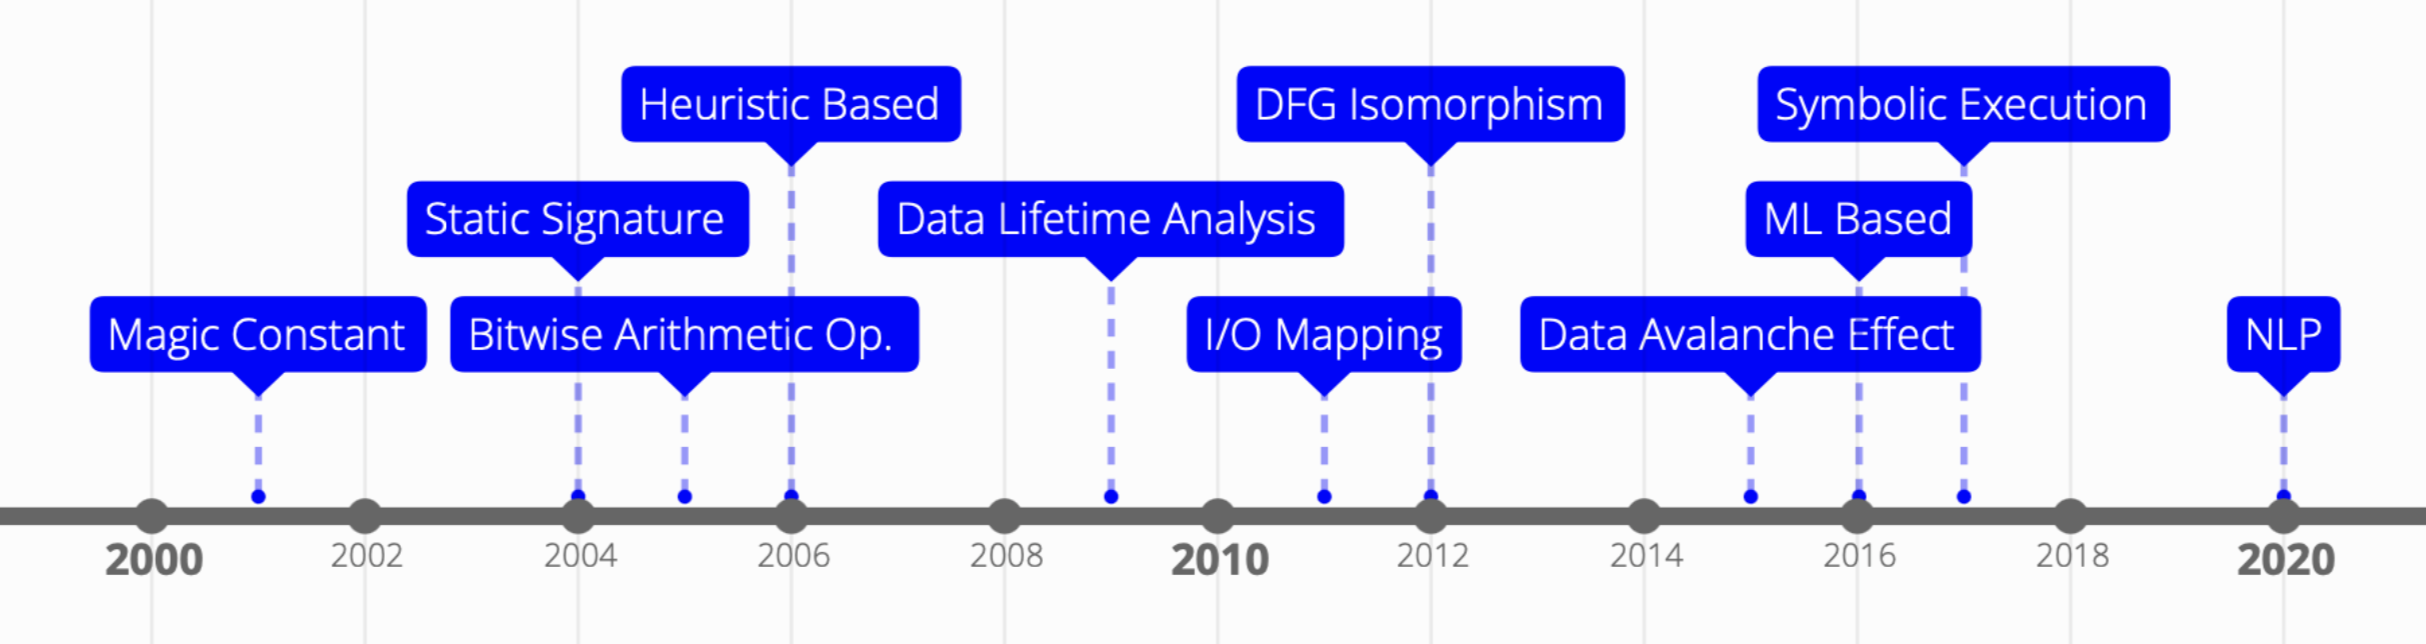
\includegraphics[width=0.95\textwidth,keepaspectratio]{ch-cryptobinary/figure/Crypto_timeline.png}
  \caption{Evolution of cryptographic function identification techniques}
  \label{fig:cryptobinary-timeline}
\end{figure}

%%4 Paragraph 3: Challenges
%However, cryptographic function identification has its own sets of challenges.
%Binaries can be obfuscated in a variety of ways, such as control-flow flattening,
%data-splitting, data-aggregation, and inclusion of bogus control-flow. In addition,
%simple cryptographic algorithms can be implemented in a variety of ways, hence
%detection mechanism that may work on one variation may fail on its more complicated (or more simplified) implementations. Malware authors also generate packed binaries to evade
%any possible detection.


While general purpose binary analysis and function identification techniques are themselves broad and thriving areas that could potentially solve these problems, a variety of work across industry and academia has focused on solving these challenges more specifically: developing techniques and tools that are uniquely tailored to identifying \textit{cryptographic primitives} in binary applications.  This allows researchers to often provide better results in different domains, leveraging cryptography-specific features.
% Paragraph 4: landscape
Cryptographic functions tend to have many mathematical computations,
nested loops, and exclusive input-output mappings which are distinct from
non-cryptographic functions and can thus be useful as a means of identification. 
% \autoref{fig:cryptobinary-timeline} shows a timeline of various techniques and approaches used in cryptographic function identification research to date.
%\priyam{taken it to the background}
Harvey et al.~\cite{harvey2001cipher} first utilized magic constants to identify
cryptographic primitives in 2001. Later works focused on signature
based detection mechanisms. However, due to the limitations of signature
based approaches, subsequent work placed a greater emphasis on heuristic based detection, such as
identification of basic blocks, instruction patterns, etc. With the
popularization of modern machine learning algorithms, newer works utilized
deep learning and AI to extract cryptographic features from a binary.
%We discuss these various approaches in depth in Section~\ref{sec:features}.

Unfortunately, while there has been a wealth of work in the space, it has generally failed to keep up with modern cryptographic
innovations and applications, as well as current software engineering and optimization techniques.
This can be difficult to notice as there is no standardized benchmarking or comparison framework, and individual works tend to test on algorithms that they are best at identifying, while neglecting those they cannot.
Additionally, as many techniques are tailored for specific cryptographic algorithms, architectures, or settings, which change rapidly over time, reproducing past results can be challenging, making it difficult to provide comparisons across the growing landscape as well.
%Additionally, while there have been some surveys on encryption algorithms~\cite{mushtaq2017survey} and ransomware detection/mitigation~\cite{begovic2023cryptographic, mcintosh2021ransomware, smith2022machine}, these works do not investigate the capabilities of different detection tools or the gaps in the selection of algorithms.

Given how important these tools and techniques can be for both researchers and practitioners, we aim to reproduce and replicate all existing tools to date in this domain.  In this endeavor, we also offer a comprehensive analysis that categorizes and discusses the existing body of work, highlighting the strengths, weaknesses, and techniques employed.
We also seek to help drive future research in the area by identifying potential challenges and various factors that may influence performance.
%highlighting a taxonomy of modern cryptographic algorithms and discussing features that we think could be leveraged for identification. 
To help provide for a more even comparison of existing and future work, and to identify gaps that are in need of future research, we create a benchmarking framework featuring a number of modern cryptographic primitives and applications. We then use this framework to evaluate existing work.
Finally, throughout the paper, we discuss and motivate a variety of open research problems in the space.

\subsection{Our Contributions}
Our primary contributions are:

\begin{itemize}[noitemsep,topsep=0pt]

%\item We present a systematic study of cryptographic function identification
%approaches, discussing various techniques that have been leveraged, as well as their strengths and weaknesses.

\item We conduct a thorough examination of cryptographic function identification methods, exploring the range of techniques utilized and evaluating their respective strengths and limitations.

%\item We highlight a taxonomy of modern cryptographic algorithms and discuss various features of cryptographic algorithms that can be leveraged for identification purposes.
%\item We highlight a number of features of cryptographic algorithms that can be leveraged for identification purposes.

%\item We discuss a number of challenges that modern tool developers and researchers face in the space from a software and implementation perspective, such as optimizations and non-standard implementations.

\item We create a standardized suite of performance metrics and benchmarks to evaluate the effectiveness
of current detection mechanisms and analyze existing tools based on this suite.

\item We conduct comprehensive replication and reproduction studies on all existing work.

\item We provide an in-depth analysis of our findings and categorize the tools according to their performance across various dimensions.

\item Based off of this analysis and our study of existing work, we discuss the research gaps in this domain and propose directions for future work.

%\item We propose a simple tool to identfy cryptographic functions based on the program state change \priyam{TODO: update based on the eval status}
  
%\item We present a comprehensive framework to understand the scalability and
%impact of dynamic analysis in detection mechanisms. \clg{Is this one left over from your thesis?  I'm not sure how it fits in overall with the paper.}
%\priyam{we can get rid of this part}

\end{itemize}

% \subsection{Chapter Organization} The outline of our paper is as follows.
% In Section~\ref{sec:taxonomy} we present our taxonomy of cryptographic algorithms, and in Section~\ref{sec:features} we discuss the various features of cryptographic algorithms that have been used for identification.
% In Section~\ref{sec:detection} we analyze different detection techniques and their strengths and weaknesses, and in Section~\ref{sec:challenges} we enumerate the inherent challenges in detecting and classifying cryptographic code in real-world applications.
% In Sections~\ref{sec:framework} and~\ref{sec:evaluation} we introduce our benchmarking framework and run existing tools on it to generate a fair comparison among existing work and highlight gaps in coverage.


\section{Background}
\label{sec:cryptobinary-background}
%%%%%%%%%%%%%%%%%%%%

In this section, we provide background on and a classification of detection approaches that have been employed by existing tools to date.
%To our surprise, only a limited number of tools and approaches have been developed throughout the span of more than two decades.
\autoref{fig:cryptobinary-timeline} shows the evolution timeline of various techniques and approaches used in cryptographic function identification research whereas \autoref{fig:cryptobinary-tool_timeline} shows the development timeline of all studied tools.
We also provide an overview of some of the cryptographic features that existing tools focus on, to help better understand how they work and contextualize later discussion.

\begin{figure}[t]
  \centering
  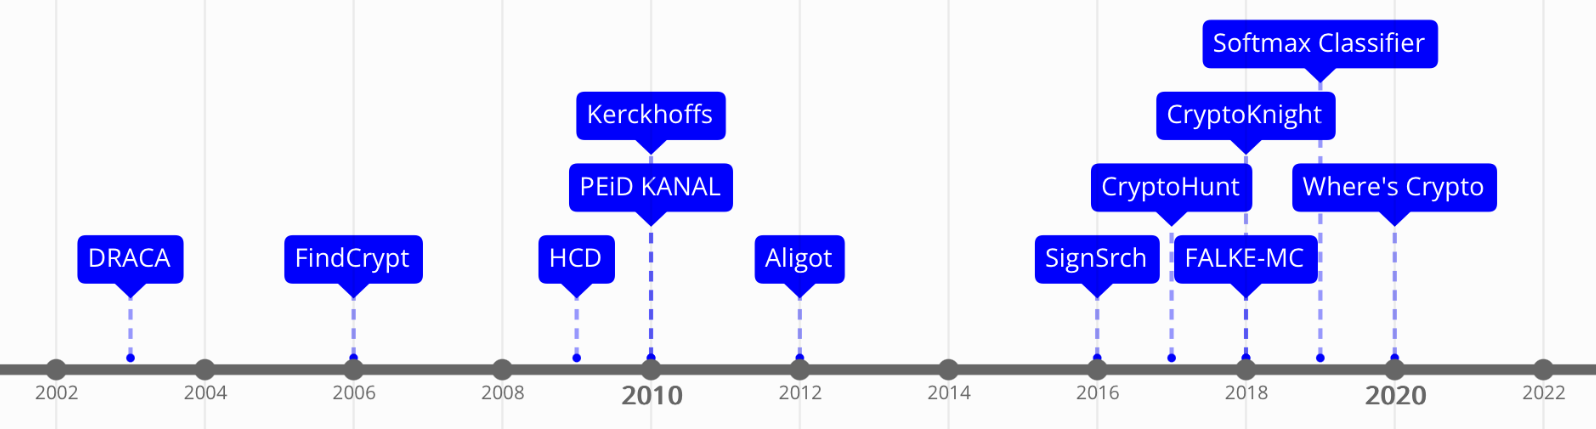
\includegraphics[width=0.95\textwidth,keepaspectratio]{ch-cryptobinary/figure/timeline.png}
  \caption{Timeline of the development of cryptographic algorithm detection tools}
  \label{fig:cryptobinary-tool_timeline}
\end{figure}

%%%%%%%%%%%%%%%%%%%%%%%%%%%%%%%%%%%%%%%%%%%%%%%%%%%%%%%%%%%%$$
\parhead{Cryptographic primitive vs. cryptographic function.} A brief note on notation used throughout this paper.  When we refer to a \textit{cryptographic function} or \textit{cryptographic algorithm}, we are generally referring to the entirety of a specific scheme or class of algorithms, such as RSA or hash functions.  When we say \textit{cryptographic primitive}, we generally mean a building block for a larger cryptographic scheme, such as a Feistel network.

%%%%%%%%%%%%%%%%%%%%%%%%%%%%%%%%%%%%%%%%%%%%%%%%%%%
\subsection{Categorization of Detection Approaches}
%%%%%%%%%%%%%%%%%%%%%%%%%%%%%%%%%%%%%%%%%%%%%%%%%%%
\label{sec:cryptobinary-detection}

Precision, scalability and performance of an identification approach all rely on the underlying techniques used.
Detection approaches can be divided into three categories:
i) Dynamic, ii) Static, and iii) Machine learning based approaches.

%%%%%%%%%%%%%%%%%%%%%%%%%%%%%%%%%

\parhead{Static Approaches.} Static approaches perform various forms of static analysis to detect
any static signatures, such as 'magic' constants, instruction sequences, and different code structures
such as S-boxes, as a means to identify cryptographic algorithms. This type of approach is based on the assumption that
cryptographic functions will perform a large number of arithmetic computations compared to non-cryptographic functions.
Harvey et al. \cite{harvey2001cipher} first proposed the idea of identifying cryptographic algorithms in binary files.
They focused on finding algorithms based on their constant
characteristics. By taking advantage of feature matching, subsequent
works \cite{lin2008automatic,caballero2007polyglot,wang2009reformat}
primarily focused on protocol reverse engineering. 
Chang et al. \cite{chang2014cryptographic} created a library of 3000 plus signature characteristics of cryptographic algorithms and also explored recognizing cryptographic algorithms based on Minimum Perfect Hash Function (MPHF).
Lestringant et al.~\cite{lestringant2015automated} used
data-flow isomorphism to find symmetric key algorithms.

Off-the-shelf tools such as Draft Crypto Analyzer
(DRACA)~\cite{draca}, Kanal~\cite{kanal}, Kerckhoffs~\cite{kerckhoffs},
Hash \& Crypto Detector (HCD)~\cite{hcd}, Signsrch~\cite{signsrch}, and Findcrypt~\cite{findcrypt2}, 
utilize static signature patterns of different cryptographic functions.
Static based approaches have low performance overhead. However, these
detection mechanisms can be easily bypassed using simple obfuscation techniques. For example,
the authors of Aligot~\cite{calvet2012aligot} showed that simple data obfuscation techniques
can bypass static analysis based detection mechanisms.

%%%%%%%%%%%%%%%%%%%%%%%%%%%%%%%%%%

\parhead{Dynamic Approaches.} Dynamic approaches~\cite{xu2017cryptographic,calvet2012aligot,li2012cipherxray}
primarily focus on identifying cryptographic primitives
from execution traces.
Lutz et al. \cite{lutz2008towards} first applied dynamic analysis to identify cryptographic algorithms based on three indicators:
i) presence of loops, ii) changes in entropy, and iii) high ratio of bitwise
arithmetic instructions.
Based on the data avalanche effect, CipherXRay~\cite{li2012cipherxray}
pinpoints the boundary of cryptographic operations and recovers transient
cryptographic secrets. However, this approach does not work in the case of stream
ciphers, for example, as they do not show any data avalanche effect.

Gr{\"o}bert et al.~\cite{grobert2011automated} proposed heuristic based 
approaches on both generic characteristics of cryptographic code and on
signatures for specific instances of cryptographic algorithms by mapping 
input-output (I/O) relations. Aligot~\cite{calvet2012aligot} further extends
this idea of I/O mapping. It retrieves
I/O parameters in an implementation-independent fashion, and compares
them with known cryptographic functions as well as performs
an interloop data flow analysis.
CryptoHunt~\cite{xu2017cryptographic} used bit-precise symbolic
loop mapping to identify cryptographic functions and applies guided fuzzing to
make the solution scalable. Park et al. \cite{park2020symmetric} proposed a hardware-assisted tracing technique to detect
symmetric-key cryptographic routines in anti-reverse engineered binaries via
recording the change of flow instructions from the CPU at run-time.
Dynamic approaches in general perform better than static based approaches in obfuscated
binaries, but suffer from much greater performance overhead.


%%%%%%%%%%%%%%%%%%%%%%%%%%%%%%%%%%%%%%%%%%%%%%%%% 

\parhead{Machine Learning Based Approaches.} With the growing popularity of machine learning, several recent works have explored utilizing such techniques.
Shin et al.~\cite{shin2015recognizing} discussed how recurrent neural networks can identify functions in binaries with greater accuracy and efficiency.
However, their approach was generalized for any function identification. 
For the purpose of cryptographic function identification,
Wright et al.~\cite{wright2009neural} proposed an artificial neural network model to classify
functional blocks as being either cryptographic or not by extracting the frequency of different logic instructions from a
disassembled program.
Benedetti et al. \cite{benedetti2017detection} used the `grap' tool to detect
cryptographic algorithms by creating patterns for AES and ChaCha20.
Falke~\cite{aigner2018falke} proposed a neural network based approach
by modeling classifiers for arbitrary cryptographic algorithms from
sample files and then automatically extracting features to train the neural
network. It offered a high detection rate in combination with
a low false positive rate.
Hill et al.~\cite{hill2018cryptoknight} proposed a Dynamic Convolutional Neural
Network based learning system (CryptoKnight) which learns from new cryptographic
execution patterns to classify unknown software.
Jia et al. \cite{jia2020neural} proposed an NLP-based approach which first extracts the
semantic information of assembly instructions and then transfers them into
100-dimensional vectors and later uses K-Max-CNN-Attention to classify
cryptographic functions.


%\parhead{Hybrid Solution.}
%\clg{This still needs to be filled out}


%\begin{figure}[h]
%	\includegraphics[width=\textwidth]{images/cryptoknight.pdf}
%	\caption{The CryptoKnight classification pipeline. 'Dynamic Binary Analysis' marked in red, is the point-of-failure.}
%\end{figure}


%The shared \texttt{CryptoTrace.so} object is built on the 32-bit \texttt{i386} architecture,
% and returns loading errors when run on \texttt{x86\_64} systems. 
 %On running the binary on an Ubuntu image running \texttt{i386}, d
 %ynamic instrumentation failed with segmentation faults, the stack trace displaying `\texttt{??? at CryptoTrace.so+0x7f550}' for every frame.


%\clg{This does not really seem relevant to the background section?  This seems like something that should maybe go in an appendix or something like that to explain why we couldn't test things?}

%\clg{I feel like background should maybe briefly introduce each tool, its techniques, and the algorithms it tries to target.  Or something like that.}
%\priyam{updated}


\subsection{Cryptographic Features}
\label{sec:cryptobinary-features}
%%%%%%%%%%%%%%%%%%%%%%%%%%%%%%%%
Cryptographic functions have their own (often quite distinct) set of characteristics, and work thus far has often leveraged these for identification, as they can lead to more tailored or performant techniques than general purpose binary analysis and code identification.
Many of these features only pertain to certain algorithms and cannot be used to identify others.
We now discuss some of the popular cryptographic features used for identification purposes.

%%%%%%%%%%%%%%%%%%%%%%%%%%%%
\parhead{Magic Constants.} In this approach, algorithm specific ``magic constants'' are searched for in the binary.  These are constant values that must occur in any implementation of a given algorithm.
%For example, the magic constants for the TEA algorithm usually are 2654435769 or
%0x9E3779B9. Existence of these constants in a binary can be used as a hint that it might contain TEA.
For instance, Signsrch~\cite{signsrch} relies on the magic number `0x9e3779b9' to detect the TEA algorithm; however, it fails to identify the algorithm when data obfuscation is applied~\cite{xu2017cryptographic}.

%%%%%%%%%%%%%%%%%%%%%%%%%%%%%%%%%
\parhead{Presence of Loops.} Most cryptographic functions use some form of loops for key generation, encryption, or other operations.
%For example, the factorization-based RSA algorithm has loops to perform modular exponentiation.
CryptoHunt~\cite{xu2017cryptographic} utilized loops as a means for detection. Given that loops may present in regular functions, further program analysis is necessary to ensure accurate detection.

%%%%%%%%%%%%%%%%%%%%%%%%%%%%%%%%%%
\parhead{Changes in Entropy.} The process of decryption usually decreases information entropy. Hence, entropy can be used as an indicator of  encrypted versus plaintext data. Several techniques~\cite{lutz2008towards, lee2022rcryptect} have used entropy to distinguish encrypted blocks from regular ones. 
However, relying on entropy can also lead to false positives in certain circumstances~\cite{grobert2011automated}.

%%%%%%%%%%%%%%%%%%%%%%%%%%%
\parhead{I/O Mapping.} Cryptographic functions sometimes have one-to-one mappings between their input to output, i.e., given a key and the plaintext, we might always get the same output, or given the input to a hash function, we should always get the same output. 
%These sort of unique one-to-one mappings can sometimes be used as indicators of the presence of cryptography (or even of specific deterministic algorithms like a hash function). 
However, these approaches rely on the accurate extraction of the key and input/output from the memory, as any wrong extraction can defeat the usefulness of unique mapping.
%data obfuscation
 
%%%%%%%%%%%%%%%%%%%%%%%%%%%%%%%%%%%%%
\parhead{Data-Flow Isomorphism.}
%A Data-Flow Graph (DFG) is a graph that represents data dependencies between a number of
%perations within a program~\cite{DFG}.
In this approach~\cite{lestringant2015automated}, a Data-Flow Graph (DFG)~\cite{DFG} is generated from the
corresponding assembly code, and subgraphs in the DFG are checked to see
whether they are isomorphic to the graph signature of a particular cryptographic
algorithm.
%This approach was first proposed by Lestringant
%et al~\cite{lestringant2015automated} and primarily used to identify symmetric
%key based algorithms. 
However, this approach is limited in the case of conditional
statements, which are more prominent in asymmetric algorithms. Additionally, DFG can
vary in effectiveness depending on data obfuscations techniques used in the implementation, such as data-splitting.

%%%%%%%%%%%%%%%%%%%%%
\parhead{S-Box.} Substitution boxes (S-Box)~\cite{sbox} are a fundamental component used in many symmetric key ciphers.
%An S-box is a table or function that swaps input bits with different bits, enhancing encryption security against attacks
%like differential and linear cryptanalysis, and often has a very distinct signature. 
For instance, the BLOWFISH algorithm
is a 64-bit block cipher that has an S-Box consisting of 1024 elements~\cite{jia2020neural} which are usually
sequentially stored in memory, allowing tools to detect BLOWFISH by locating this S-Box in memory. Similar techniques can be applied to Permutation Boxes (P-Box)~\cite{pbox}, which are methods of bit-shuffling to permute or transpose bits across S-box inputs.


%%%%%%%%%%%%%%%%%%%%%%%%%%%%%%%%%%%%
\parhead{Instruction Sequences.} An instruction sequence is a series of instructions or commands that a CPU executes in a specific order to perform tasks within a program. %These instructions can range from simple arithmetic calculations to more complex data manipulation and control flow operations. 
Many fundamental cryptographic operations will consist of fingerprintable instruction sequences and hence can be used for the purpose of identification. Nevertheless, this method may lose its effectiveness when dealing with control-flow obfuscations such as control-flow flattening~\cite{cfg_f}.




\subsection{Applications with Modern Cryptographic Algorithms}

Transport Layer Security (TLS) is a cryptographic protocol that is specifically crafted to facilitate secure communication over networks.

Starting from TLS 1.1, elliptic curve cryptography (ECC) has been incorporated into the TLS protocol. Furthermore, in TLS 1.3, ECC takes a central role in the base specification, featuring new signature algorithms, while RSA support has been discontinued. As of 2021, the deprecation of TLS 1.0 and 1.1 has taken place, resulting in ECC as the major choice for TLS ciphersuites.

There are numerous libraries that implement TLS, including OpenSSL, cryptlib, and Java Secure Socket Extension. Concurrently, beyond the TLS, a number of other applications leverage modern cryptographic algorithms. Notable examples include iMessage and Signal, both of which implement end-to-end encryption for enhanced security.


\section{Overview}
\label{sec:cryptobinary-overview}

This paper focuses on comprehensive replication and reproduction studies for existing work on identifying cryptography code in binary applications.
To aid in this, we propose a novel analysis framework aimed at facilitating a comprehensive evaluation of cryptographic function detection tools' replicability. Our framework is introduced in \autoref{sec:cryptobinary-framework}. Subsequently, we conduct two evaluations: a reproducibility evaluation in \autoref{sec:cryptobinary-reproduction}, and a replicability evaluation in \autoref{sec:cryptobinary-replication}. Additionally, we provide further discussion on the results of our reproducibility and replicability evaluations, as well as point out a number of important takeaways and directions for future work, in \autoref{sec:cryptobinary-discussion}. Finally, to support future research in this domain, we present a summary cryptographic detection approaches and tools in \autoref{sec:cryptobinary-background} as part of our background.

%%%%%%%%%%%%%%%%%%%%%%%

\subsection{Cryptographic Algorithm Detection Tools}

A number of cryptographic detection tools have been developed based on the different approaches discussed in \autoref{sec:cryptobinary-detection}. We perform our reproduction and replication studies on all existing work that we were able to find from 2000 until now:
\vspace*{-10pt}
\setlength{\columnsep}{-20pt}
\begin{multicols}{2}
\begin{itemize}[noitemsep,topsep=0pt]
    \setlength{\itemsep}{0pt}
    \setlength{\parskip}{0pt}
\item Aligot \cite{calvet2012aligot}
\item CryptoHunt \cite{xu2017cryptographic}
\item CryptoKnight \cite{hill2018cryptoknight}
\item DRACA \cite{draca}
\item FindCrypt2 \cite{findcrypt2}
\item FALKE-MC \cite{aigner2018falke}
\item HCD \cite{hcd}
\item Kerckhoff \cite{kerckhoffs}
\item PEiD KANAL \cite{kanal}
\item SignSrch \cite{signsrch}
\item Softmax Classifier \cite{jia2020neural}
\item Where's Crypto \cite{meijer2021s}
\end{itemize}
\end{multicols}
\vspace*{-5pt}
Our focus is on evaluating tools specifically designed for identifying cryptographic functions and comparing these tools with their stated performance. As such, we exclude other (broader) binary analysis tools, such as Binshape \cite{shirani2017binshape}, a general-purpose binary analysis tool, or CIS \cite{matenaar2012cis}, which focuses on testing cryptographic heuristics rather than actual algorithms.

We also employ a systematic approach to categorize, classify, and interrelate the diverse array of knowledge elements that constitute such tools from several directions in \autoref{subsec:cryptobinary-tool_cat}. We provide a more detailed discussion of each tool, along with its strengths and weaknesses, in \autoref{app:cryptobinary-tools}.

We comprehensively summarize the detection abilities of each cryptographic function detection tool. We did a thorough check of each tool's documents and signatures to see what types of cryptographic algorithms they can find. \autoref{fig:cryptobinary-percentage} shows the distribution of various algorithms that existing work has focused on.
After that, we gather all the information we found and explain it in more detail in \autoref{tab:cryptobinary-summary}. This helps us better understand what each tool can do in terms of detecting different cryptographic algorithms.

\begin{table*}[]
\centering
\setlength{\tabcolsep}{4pt}
\begin{adjustbox}{max width=\textwidth}
\renewcommand{\arraystretch}{1.5}
\begin{tabular}{l||c|c|c|c|c|c|c|c|c|c|c|c}
\hline
Tool & Aligot & \begin{tabular}[c]{@{}c@{}}Crypto-\\ Hunt\end{tabular} & \begin{tabular}[c]{@{}c@{}}Crypto-\\ Knight\end{tabular} & DRACA & FindCrypt2 & FALKE-MC & HCD & Kerckhoff & \begin{tabular}[c]{@{}c@{}}PEiD\\ KANAL\end{tabular} & SignSrch & \begin{tabular}[c]{@{}c@{}}Softmax\\ Classifier\end{tabular} & \begin{tabular}[c]{@{}c@{}}Where's\\ Crypto\end{tabular} \\ \hline\hline

ADLER32 &  &  &  &  &  &  & \multirow{35}{*}{\rotatebox[origin=c]{90}{\textit{Not Available}}} &  & \multirow{35}{*}{\rotatebox[origin=c]{90}{\textit{Not Available}}} &  & \cmark &  \\ \cline{1-7} \cline{9-9} \cline{11-13}
AES (Rijndael) & \cmark & \cmark & \cmark & \cmark & \cmark & \cmark &  & \cmark &  & \cmark &  & \cmark \\ \cline{1-7} \cline{9-9} \cline{11-13}
BASE64 &  &  &  &  &  &  &  &  &  & \cmark & \cmark &  \\ \cline{1-7} \cline{9-9} \cline{11-13}
Blowfish &  &  & \cmark & \cmark & \cmark &  &  &  &  & \cmark & \cmark &  \\ \cline{1-7} \cline{9-9} \cline{11-13}
Camellia &  &  &  &  & \cmark &  &  &  &  &  &  &  \\ \cline{1-7} \cline{9-9} \cline{11-13}
CAST &  &  &  &  & \cmark &  &  &  &  & \cmark &  &  \\ \cline{1-7} \cline{9-9} \cline{11-13}
CAST-256 &  &  &  & \cmark & \cmark &  &  &  &  & \cmark &  &  \\ \cline{1-7} \cline{9-9} \cline{11-13}
CRC32 &  &  &  & \cmark & \cmark &  &  &  &  & \cmark & \cmark &  \\ \cline{1-7} \cline{9-9} \cline{11-13}
DES &  &  &  & \cmark & \cmark &  &  & \cmark &  & \cmark & \cmark & \cmark \\ \cline{1-7} \cline{9-9} \cline{11-13}
EC &  &  &  &  &  &  &  &  &  & \cmark &  &  \\ \cline{1-7} \cline{9-9} \cline{11-13}
GOST &  &  &  &  & \cmark &  &  &  &  & \cmark &  &  \\ \cline{1-7} \cline{9-9} \cline{11-13}
HAVAL &  &  &  &  & \cmark &  &  &  &  & \cmark & \cmark &  \\ \cline{1-7} \cline{9-9} \cline{11-13}
MARS &  &  &  & \cmark & \cmark &  &  &  &  & \cmark &  &  \\ \cline{1-7} \cline{9-9} \cline{11-13}
MD2 &  &  &  &  & \cmark &  &  &  &  & \cmark &  &  \\ \cline{1-7} \cline{9-9} \cline{11-13}
MD4 &  &  &  &  & \cmark &  &  &  &  & \cmark &  &  \\ \cline{1-7} \cline{9-9} \cline{11-13}
MD5 & \cmark & \cmark & \cmark & \cmark & \cmark &  &  & \cmark &  & \cmark & \cmark & \cmark \\ \cline{1-7} \cline{9-9} \cline{11-13}
RC2 &  &  &  & \cmark & \cmark &  &  &  &  & \cmark &  &  \\ \cline{1-7} \cline{9-9} \cline{11-13}
RC4 & \cmark & \cmark & \cmark &  &  & \cmark &  & \cmark &  &  &  &  \\ \cline{1-7} \cline{9-9} \cline{11-13}
RC5 &  &  &  & \cmark & \cmark &  &  &  &  & \cmark & \cmark &  \\ \cline{1-7} \cline{9-9} \cline{11-13}
RC6 &  &  &  & \cmark & \cmark &  &  &  &  & \cmark & \cmark &  \\ \cline{1-7} \cline{9-9} \cline{11-13}
Ripemd-160 &  &  &  & \cmark &  &  &  &  &  & \cmark &  &  \\ \cline{1-7} \cline{9-9} \cline{11-13}
RSA & \cmark & \cmark & \cmark &  &  &  &  & \cmark &  &  &  &  \\ \cline{1-7} \cline{9-9} \cline{11-13}
SAFER &  &  &  & \cmark & \cmark &  &  &  &  & \cmark &  &  \\ \cline{1-7} \cline{9-9} \cline{11-13}
SHA-1 &  &  &  & \cmark & \cmark &  &  &  &  & \cmark & \cmark & \cmark \\ \cline{1-7} \cline{9-9} \cline{11-13}
SHA-256 &  &  &  &  & \cmark &  &  &  &  & \cmark & \cmark & \cmark \\ \cline{1-7} \cline{9-9} \cline{11-13}
SHA-512 &  &  &  &  & \cmark &  &  &  &  & \cmark &  & \cmark \\ \cline{1-7} \cline{9-9} \cline{11-13}
SHARK &  &  &  &  & \cmark &  &  &  &  & \cmark &  &  \\ \cline{1-7} \cline{9-9} \cline{11-13}
Skipjack &  &  &  & \cmark & \cmark &  &  &  &  & \cmark &  &  \\ \cline{1-7} \cline{9-9} \cline{11-13}
Square &  &  &  &  & \cmark &  &  &  &  & \cmark &  &  \\ \cline{1-7} \cline{9-9} \cline{11-13}
TEA & \cmark & \cmark &  & \cmark &  &  &  &  &  & \cmark &  &  \\ \cline{1-7} \cline{9-9} \cline{11-13}
Tiger &  &  &  & \cmark & \cmark &  &  &  &  & \cmark &  &  \\ \cline{1-7} \cline{9-9} \cline{11-13}
Twofish &  &  &  & \cmark & \cmark &  &  &  &  & \cmark &  &  \\ \cline{1-7} \cline{9-9} \cline{11-13}
WAKE &  &  &  &  & \cmark &  &  &  &  & \cmark &  &  \\ \cline{1-7} \cline{9-9} \cline{11-13}
Whirlpool &  &  &  &  & \cmark &  &  &  &  & \cmark &  &  \\ \cline{1-7} \cline{9-9} \cline{11-13}
XTEA &  &  &  &  &  &  &  &  &  &  &  & \cmark \\ \hline
\end{tabular}
\end{adjustbox}
%}
\caption{Cryptographic algorithm detection support as stated in the paper or documentation for each tool}
\label{tab:cryptobinary-summary}
\end{table*}

Note that we compiled these results based on information provided by the developers of each tool. Through our comprehensive analysis, we found that commercial tools like DRACA~\cite{draca}, FindCrypt2~\cite{findcrypt2}, and Signsrch~\cite{signsrch} can detect a diverse range of cryptographic algorithms. However, their performance falter when encountering obfuscation or atypical situations. Certain academic-developed tools such as Aligot~\cite{calvet2012aligot},  CryptoHunt~\cite{xu2017cryptographic}, and Where's Crypto~\cite{meijer2021s} offer superior analysis results in specific scenarios, such as detecting cryptographic algorithms from obfuscated binaries. Many of them can only detect a few cryptographic algorithm, but they can be easily expanded.

It is important to recognize that a simple summary may not fully capture the current capabilities and detection abilities of each tool. Moreover, many of these tools were developed years ago, and they may not be compatible with current programming languages, compilers, and/or hardware architectures.  This is why our reproduction and replication study is so crucial.  It not only highlights these major gaps in existing work as the space has progressed, but allows us to provide insights on the space more broadly, and on a variety of important avenues for future work.

\begin{figure}[t]
    \centering
    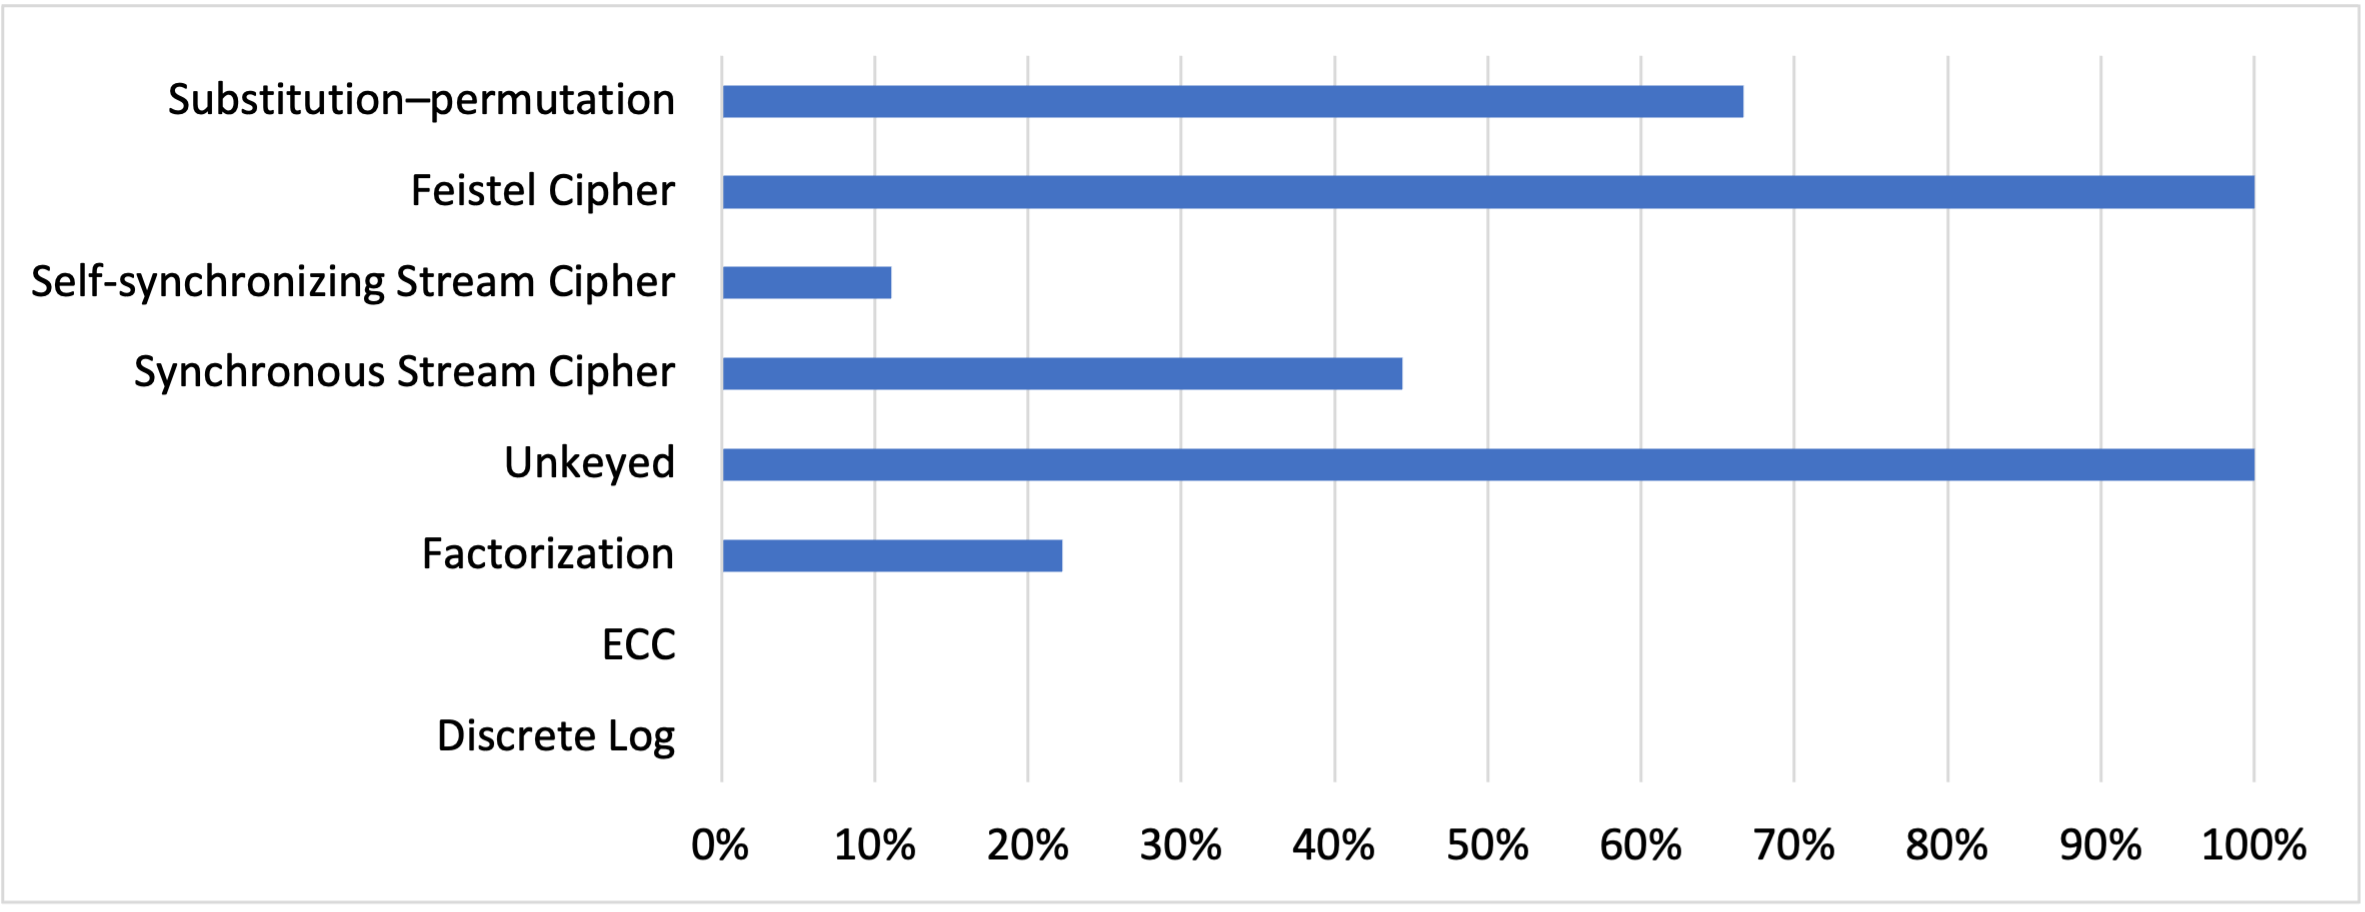
\includegraphics[width=0.95\textwidth]{ch-cryptobinary/figure/algo_percentage.png}
		\caption{Types of cryptographic functionality and designs targeted by different tools and approaches, by percentage of tools surveyed}
		\label{fig:cryptobinary-percentage}
\end{figure}

% \fanyo{To gain a comprehensive understanding of the current state of cryptographic function detection techniques and related tools, we conducted a comprehensive investigation experiment. We introduced numerous new evaluation benchmarks and frameworks that previous research in this field has not explored. Our benchmark will be detailed in Section \ref{sec:framework}, while the experiment results will be presented in Section \ref{sec:evaluation}. Additionally, we will provide discussion based on our evaluation results in Section \ref{sec:discussion}.}




% \fanyo{To gain a comprehensive understanding of the current state of cryptographic function detection techniques and related tools, we conducted a comprehensive investigation experiment. We introduced numerous new evaluation benchmarks and frameworks that previous research in this field has not explored. Our benchmark will be detailed in Section \ref{sec:framework}, while the experiment results will be presented in Section \ref{sec:evaluation}. Additionally, we will provide discussion based on our evaluation results in Section \ref{sec:discussion}.}






% %%%%%%%%%%%%%%%%%%%%%%%%%%%%%%%%%
% \subsection{Research Questions}
% %%%%%%%%%%%%%%%%%%%%%%%%%%%%%%%%%

% We also work to understand how well state-of-the-art techniques and tools perform by proposing and answering the following research questions.  We also believe many of these research questions are still yet unanswered in a satisfactory way, as we discuss more in Section~\ref{sec:evaluation} where we present a number of open research problems in these directions.

% \begin{itemize}
%   \item \textbf{R1} Does the choice of compiler play a role in the detection success? 
%   \item \textbf{R2} Is there any impact from optimization flags?
%   \item \textbf{R3} Are some algorithms easier to detect compared to others? 
%   \item \textbf{R4} Can the same tool perform similarly well across different algorithms?
%   \item \textbf{R5} Is the version of the algorithm significant during detection? 
%   \item \textbf{R6} Are ``malicious'' versions of cryptographic algorithms trickier to detect?

% \end{itemize}




\subsection{Categorization of Cryptographic Algorithm Detection Tools}
\label{subsec:cryptobinary-tool_cat}

We employ a systematic approach to categorize, classify, and interrelate the diverse array of knowledge elements that constitute such cryptographic detection tools from several directions. \autoref{tab:cryptobinary-taxonomy1} contains an overview and summary of each tool, including its reproduction and replication status in this work, as well as a variety of information such that one can easily find or organize existing (and future) tools based on the per-column categories.

We begin by categorizing the detection approach (broken down by the different methods discussed previously in ~\autoref{sec:cryptobinary-detection}) and the programming language in which the tool's source code is written. We note that some tools are not open source; they provide only an executable file, and as a result, we lack information about the source language.
Some tools require specific dependent libraries to run, which can limit or hinder their usability, and as such we list if there are any required dependencies.
Some tools are installation-free and do not require compilation, offering an easy, user-friendly experience.
And a few tools provide the capability for developers to insert new cryptographic algorithm signatures, thereby expanding their detection capabilities as the field advances.
 
\begin{sidewaystable}[p]
\centering
\footnotesize
\renewcommand{\arraystretch}{1.75}

\begin{adjustbox}{max width=0.9\textheight}
\begin{tabular}{c||c|c|c|c|c|c|c|c}
\hline
Tool & Method & \begin{tabular}{@{}c@{}}Dependent\\[-6pt]Library\end{tabular} & Language & \begin{tabular}{@{}c@{}}Requires\\[-6pt]Compiling\end{tabular} & Expandable & R+R & \begin{tabular}{@{}c@{}}Obf. Binary\\[-6pt]Design\end{tabular} & \begin{tabular}{@{}c@{}}AI/ML\\[-6pt]Approach\end{tabular} \\ \hline
\hline
Aligot         & I/O Parameters             & Intel Pin          & Python     & Yes     & Yes     & Reproducible & No  & No  \\ \hline
CryptoHunt     & Bit-precise Symbolic Loop  & Intel Pin          & C++        & Yes     & Yes     & Unable       & Yes & No  \\ \hline
CryptoKnight   & Machine Learning Based     & Intel Pin, PyTorch & Python     & Yes     & Yes     & Both         & No  & Yes \\ \hline
DRACA          & Unknown                    & None               & Executable & No      & No      & Replicable   & No  & No  \\ \hline
FindCrypt2     & Magic Constants            & IDA Pro            & C++        & Yes     & No      & Replicable   & No  & No  \\ \hline
FALKE-MC       & Neural Network             & None               & Unknown    & Unknown & Unknown & Unable       & Yes & Yes \\ \hline
HCD            & Unknown                    & None               & Executable & No      & No      & Replicable   & No  & No  \\ \hline
Kerckhoff      & Multiple                   & Intel Pin          & Python     & No      & Yes     & Unable       & No  & No  \\ \hline
PEiD KANAL     & Signature Searching        & None               & Executable & No      & Yes     & Replicable   & No  & No  \\ \hline
Signsrch       & Signature Searching        & None               & Executable & No      & No      & Replicable   & No  & No  \\ \hline
Softmax Classifier & Neural Network         & Unknown            & Python     & Unknown & Unknown & Unable       & No  & Yes \\ \hline
Where's Crypto & DFG Isomorphism            & IDA SDK            & C++        & Yes     & Yes     & Both         & No  & No  \\ \hline
\end{tabular}
\end{adjustbox}

\caption{Categorization of existing tools and their important properties}
\label{tab:cryptobinary-taxonomy1}
\end{sidewaystable}
\section{Analysis Framework for Open-Source Detection Tools}
%%%%%%%%%%%%%%%%%%%%%%%%%%%%%%%%%%%%%%%%%%%%%%%%%%%%%%%%%%%
\label{sec:cryptobinary-framework}

Previous tools have been evaluated only with certain basic cryptographic algorithms, and often seem to lack evaluation for false positives, real world applications, and large scale projects. Therefore, as the first step in our replication study, we build a new benchmarking framework with a number of evaluation metrics, which will not only encompass all evaluations conducted by previous tools but also establish a unified more comprehensive evaluation benchmark moving forward.

\fanyo{add transaction}

\vspace*{-10pt}
\begin{multicols}{3}
\begin{itemize}[noitemsep,topsep=0pt]
\item Aligot \cite{calvet2012aligot}
\item CryptoHunt \cite{xu2017cryptographic}
\item CryptoKnight \cite{hill2018cryptoknight}
\item DRACA \cite{draca}
\item FindCrypt2 \cite{findcrypt2}
\item HCD \cite{hcd}
\item PEiD KANAL \cite{kanal}
\item SignSrch \cite{signsrch}
\item Where's Crypto \cite{meijer2021s}
\end{itemize}
\end{multicols}
\vspace*{-10pt}

\subsection{Benchmarking Framework}
\label{subsec:cryptobinary-framework}
%%%%%%%%%%%%%%%%%%%
During our study, we identified a significant gap in the field: the absence of a standardized method for evaluating existing tools and their efficacy.
We believe that to do a fair evaluation in any domain requires a standard
benchmark. We propose a benchmarking framework that will help us understand the scalability
and effectiveness of any given detection approach. We have four categories in our framework: i) basic cryptographic functions, ii) microbenchmarks, iii) libraries, and iv) large projects.
Our framework is flexible and can be easily updated as the field of cryptography advances. 

\parhead{Basic cryptographic functions.} The basic cryptographic functions category contains cryptographic algorithms from various standard classes within the cryptographic space. A single cryptographic algorithm may have multiple versions, or may use non-standard implementations, so we may select many different implementations or versions for certain algorithms. The cryptographic algorithms we select are:

\vspace*{-10pt}
\begin{multicols}{3}
\begin{itemize}[noitemsep,topsep=0pt]
\item AES256
\item DES
\item ECC
\item MD5
\item RC4 
\item RC5
\item RSA
\item SHA1
\item SHA256
\item TEA
\item XTEA
\item XXTEA
\end{itemize}
\end{multicols}
\vspace*{-10pt}

We have chosen these algorithms for several reasons. First, we have included those recommended by the National Institute of Standards and Technology (NIST) \cite{nist}, as they are widely utilized and cover a broad range of real-world applications. Second, we have incorporated algorithms like TEA and MD5, which, although once popular, are now considered unsafe or outdated, but still might have historical significance in applications like malware. Last, we have selected various variants of a single cryptographic algorithm to assess a tool's ability to handle different implementations effectively.

\parhead{Microbenchmarks.} Our microbenchmarks category contains small programs on file
manipulation, networking, I/O heavy programs, math heavy programs, matrix and array, and so-called ``golden
implementations'' of well-known cryptographic algorithms. We have chosen small
programs such as I/O heavy and math-heavy programs since they have similar
instruction sets or behavior patterns as cryptographic functions.  This allows us to test for false positives in a detection framework.

\parhead{Libraries.} We have chosen cryptographic libraries as well as encoding and
compression libraries that have similar behavior to cryptographic
functions including:
\vspace*{-10pt}
\begin{multicols}{2}
\begin{itemize}[noitemsep,topsep=0pt]
\item openssl (3.3.1)
\item libgcrypt (1.8.11)
\item libsodium (1.0.20)
\item mbedTLS (3.6.1)
\item gnuTLS (3.8.6)
\item bzip2 (1.0.8)
\item zlib (1.3.1)
\item ffmpeg (7.0.2)
\item libgsm (1.0.17)
\item libjpeg (6b)
\item libpng (1.6.43)
\end{itemize}
\end{multicols}

This allows us to again test for false positives, but also to test for a variety of different cryptographic algorithms implemented in different ways.
We select open source libraries only, so that we are able to compile them based on our evaluation metrics. For each tool, we used the latest version available at the time of evaluation. Our selection includes a diverse range of libraries, from those with frequent recent updates, such as OpenSSL, to those that are a bit older, such as libjpeg.

\parhead{Large projects.} We also select Signal, an application designed for encrypted messaging, to evaluate a tool's ability to both scale for large codebases as well as still detect cryptography within them.  We believe that to understand the scalability of a mechanism, it is crucial to determine that the tool performs well irrespective of the code size and its applications.
Signal was selected because it both utilizes multiple (modern) cryptographic schemes and is open source.  This again means we can recompile Signal with our evaluation metrics, plus establish ground truth for testing. However, as our framework is open-source, one could easily extend it to include any future desired large-scale open-source projects, such as Tor.

\subsection{Evaluation Metrics}
\label{subsec:cryptobinary-metrics}
To ensure a thorough exploration of current tools (and to provide rigorous and fair evaluation metrics for the future), we have meticulously crafted a series of evaluation experiments. These experiments are thoughtfully designed to align with the challenges we discuss in \autoref{subsec:cryptobinary-challenges}, maximizing our ability to uncover the current state of these tools and elucidate their strengths and weaknesses.  Our evaluation metrics are as follows:
 
\begin{itemize}
\item \textbf{Based on optimization levels:} Evaluate based on different compiler optimizations including \texttt{-O0}, \texttt{-O1}, \texttt{-O2}, \texttt{-O3}, \texttt{-Os}, and \texttt{-Ofast}.

\item \textbf{Based on different combinations of obfuscation mechanisms:}

\begin{itemize}
\item \textbf{Control-flow obfuscation:} Adding bogus control-flow, control-flow flattening, substitution of instructions, polymorphism.

\item \textbf{Data-flow obfuscation:} Data aggregation, data-splitting, variable transformation.

\item \textbf{Modified versions of algorithms:} For example, modified TEA (Russian TEA) used in malware as suggested in \cite{xu2017cryptographic}.

\item \textbf{Layout Obfuscation:} Address obfuscation, obfuscating debug information, address layout/memory layout randomization .

\item \textbf{Combination of prior techniques}
\end{itemize}
% \item \textbf{Based on type of the algorithm:} Some approaches can work better on stream ciphers, some others can work better on block ciphers

\item \textbf{Based on different compilers:} Evaluate based on different compilers, including GCC, CLANG, MSVC.
% \item \textbf{Based on algorithm versions:} A single cryptograhic algorithm may have multiple variant versions, and some malware do not use standard algorithm implementation.

\end{itemize}

The full list of optimizations, obfuscations, and their combinations selected for our evaluation is shown below.

\begin{enumerate}
\setcounter{enumi}{-1}
\item No identification
\item Identification with optimization flag \texttt{-O0}
\item Identification with optimization  flag \texttt{-O1}
\item Identification with optimization flag \texttt{-O2}
\item Identification with optimization flag \texttt{-O3}
\item Identification with optimization flag \texttt{-Os}
\item Identification with optimization flag: \texttt{-Ofast}
\item Identification with instruction substitution obfuscation: \texttt{-obs\textunderscore sub}
\item Identification with control-flow flattening: \texttt{-obs\textunderscore fla}
\item Identification with bogus control-flow: \texttt{-obs\textunderscore bcf}
\item Identification with combination of obfuscation: \texttt{-obs\textunderscore sub}, \texttt{-obs\textunderscore fla}, \texttt{-obs\textunderscore bcf}
\item Identification with combination of obfuscation and optimization: \texttt{-obs\textunderscore sub}, \texttt{-obs\textunderscore fla}, \texttt{-obs\textunderscore bcf}, \texttt{-O3}
\end{enumerate}

%\section{Identiifcation techniques}
%%%%%%%%%%%%%%%%%%%%%%%%%%%%%%%%%%%


%%%%%%%%%%%%%%%%%%%%%%%%%%%%%%%
%\begin{figure}[ht]
%\centering{
%  \subfigure[Evaluation of DRACA based on performance metrics]{%
%    \includegraphics[width=\columnwidth, keepaspectratio]{./images/draca.pdf}
%    \label{fig:draca}}
%  \subfigure[Evaluation of Signsrch based on performance metrics]{%
%    \includegraphics[width=\columnwidth, keepaspectratio]{./images/signsrch.pdf}
%    \label{fig:signsrch}}
%    %\caption{}
%}
%\end{figure}

% \begin{figure}[ht]
% \centering
% \begin{minipage}{.45\textwidth}
%   \centering
%   \includegraphics[width=\linewidth]{./images/draca.pdf}
%   \caption{Evaluation of DRACA based on performance metrics}
%   \label{fig:draca}
% \end{minipage}%
% \qquad
% \begin{minipage}{.45\textwidth}
%   \centering
%   \includegraphics[width=\linewidth]{./images/signsrch.pdf}
%   \caption{Evaluation of Signsrch based on performance metrics}
%   \label{fig:signsrch}
% \end{minipage}
% \end{figure}

We assessed each tool with these benchmarks and metrics to thoroughly explore accuracy and detection capabilities when handling binary programs subjected to specific compiler or optimization/obfuscation techniques.\footnote{All benchmarks and metrics we evaluate are available at \url{https://github.com/BARC-Purdue/CryptoBinary}.} For instance, a tool \textbf{A} might successfully detect MD5 when all optimization flags are applied but fail to do so in the presence of obfuscation. Conversely, a tool \textbf{B} may be able to detect TEA when compiled with GCC but not when compiled with CLANG. This exploration provides us with a more comprehensive understanding of the current state of cryptographic function detection tools, revealing their weaknesses and indicating areas for future development from various perspectives.


% Then based on our metric, we give tool \textbf{A}
% score of 7 in unkeyed category. \autoref{fig:draca} and \autoref{fig:signsrch}
% shows the performance of the two tools namely DRACA and Signsrch based on
% the above mentioned metrics.





% \subsection{A Benchmark Framework}
% % For large scale project, we have chosen signal given its large code base and
% % wide spread usage. \autoref{benchmarks} shows the analysis of two tools DRACA
% % and signsrch across all the three categories of the benchmarks as well as with
% % different compilation and obfuscation flags.

% We categorized our framework in couple of directions. We can categorize them based on size to understand the scalability of each of the investigated tools. Then, we can categorize based on the type of the suite. Here are four possible categorizations: 

% \textbf{i. In accordance to size:} We can evaluate different types of projects based on size to understand  the effectiveness of tool 

% a. Micro-benchmarks  

% b. Small/ medium sized projects

% c. Large projects

% \textbf{ii. In accordance to type:} We can develop a number of test-suites which shows crypto like behavior. Possible options are: network-heavy test-suite, mathematics-heavy suite, binary packing, suite with extraction operations.

% \textbf{iii. Real world open-source projects:} We can select a good number of real world open source projects to understand the effectiveness of investigated tools.

% \textbf{iv. Real malware samples:} Possible malware: wannacry (Windows encryption API), petya, not-petya, locky (RSA-2048 + AES-128 cipher with ECB mode), Annabele (AES256 CBC with a hardcoded key and IV). Petya and NotPetya both read the MBR and encrypt it using a simple XOR key. The only difference is that Petya uses 0x37 as a key, while NotPetya uses 0x07.


%algorithm vs functionalities 


\section{Reproduction}
\label{sec:cryptobinary-reproduction}
% To verify the reproducibility and replicability for each tool, we conduct a end-to-end evaluation experiment as the following procedure
% \begin{itemize}
%   \item Compile the tool's source code from sketch in different operating system (Windows, Mac OS, and Linux) if source code is provided
%   \item Evaluate the benchmark provided by original tool if provided.
%   \item Evaluate each tool with our new  benchmark system
% \end{itemize}

We start by assessing the reproducibility of each tool by employing consistent experimental setups, procedures, and operating conditions to replicate their purported capabilities. 

In our reproducibility evaluation we follow the ACM guidelines on reproducibility \cite{rar}, using the same measurement procedure, system setting, and operating conditions as the tool's original test cases\footnote{For the precise details and steps of our reproducibility evaluation see Appendix \ref{app:cryptobinary-repro_procedure}.}. This will help us to understand the basic fundamental reliability for each tool.  When tools do not pass the reproduction evaluation, we also provide a brief discussion for why.
\autoref{tab:cryptobinary-reproducibility} shows the reproducibility results.
% \fanyo{We use \cmark to indicate successful reproduction of the tool with their original test cases, \xmark for failure to reproduce or when the tool is unavailable (neither source code nor compiled binary is provided), and \texttt{n/a} if the tool is executable but lacks the original test cases.}

\begin{table}[h]
\centering
\begin{adjustbox}{max width=\textwidth}
\begin{tabular}{c|c|c|c|c|c}
\hline
Aligot & \makecell{Crypto\\Hunt} & \makecell{Crypto\\Knight}  & DRACA  & FindCrypt2  & FALKE-MC \\ \hline
\cmark & \xmark & \cmark & \textminus & \textminus & \xmark  \\ \hline \hline
HCD & Kerckhoff  & \makecell{PEiD \\ KANAL}  & SignSrch  & \makecell{Softmax \\ Classifier}  & \makecell{Where’s \\ Crypto}\\ \hline
\textminus  & \xmark & \textminus & \textminus & \xmark & \cmark  \\ \hline
\end{tabular}
\end{adjustbox}
\caption{Reproducibility outcome for each tools. \cmark~indicates a tool that has passed the reproduction evaluation, while \xmark~represents a tool that has either failed the reproduction evaluation or is not accessible. \textminus~denotes a tool that is available for use, but the developer has not provided the original test cases.}
\label{tab:cryptobinary-reproducibility}
\vspace{-10pt}
\end{table}

Note that for certain tools, the developers only provided the executable binary program without the accompanying source code or test cases necessary for evaluation, making a reproducibility assessment unfeasible (denoted \textminus). Some tools are not publicly available in either source code or executable binary form, making a reproducibility evaluation impossible. As a result, they are marked with a \xmark. Additionally, we encountered crashes when running Pin-based tools with the latest version of Intel Pin, indicating that the design of older cryptographic detection tools may not be compatible with newer Pin versions. However, Aligot is the one exception to this.  Aligot provides step-by-step test cases, and, based on this, we have successfully reproduced each step with the expected results. Therefore, we consider Aligot reproducible, as we were able to replicate the test results using their original measurement procedures.

\subsection{Non-Reproducible Tools}
\parhead{CryptoHunt} has been successfully executed, but we are unable to provide the complete benchmarking framework and performance evaluation results. CryptoHunt detects cryptographic functions in binary code through a bit-precise symbolic loop mapping approach. However, depending on the binary's size, CryptoHunt may identify up to 10,000 loops within the binary. Without additional filtering, the process of comparing each of these loops with reference loops becomes exceedingly time-consuming and infeasible.

\parhead{Kerckhoff} cannot be evaluated in this paper due to its incompatibility with existing available versions of the Pin tracing tool, which cause it to crash. We have encountered a similar issue in the replication evaluation as well, which will be discussed in \autoref{sec:cryptobinary-replication}.
%This issue may be similar to the experience we have with Aligot, which informs future researchers that detection tools developed to depend on specific tracing functionalities may not age well or be suitable for current/future binary programs. \clg{Also not sure what you mean here with Aligot since that one worked? Also check what I rephrased here.}

\parhead{Softmax Classifier \textnormal{and} FALKE-MC} cannot be evaluated in this paper since they are not available for public use, as neither the source code nor the compiled binary is provided. Only the original research paper is available, with no accompanying software or executable.

\section{Replication}
\label{sec:cryptobinary-replication}

We now undertake a comprehensive replicability evaluation of existing work across different categories of cryptographic algorithms with our newly proposed analysis framework, in order to understand their consistency, robustness, and effectiveness. Our replication evaluation follows the ACM guidelines on replicability \cite{rar}. We rebuild each tool (if the source code is available) and run it across different system environments using our newly developed evaluation benchmark as the test cases\footnote{For the precise details and steps of our replicability evaluation see Appendix \ref{app:cryptobinary-repli_procedure}.}.
This evaluation encompasses all work across this domain, allowing us to delve into their performance and potential limitations. For each cryptographic algorithm, we considered different optimization/obfuscation levels, compilers, and implementations. These experiments are designed to help us understand the consistency and robustness of existing work and techniques, the current status of cryptographic function detection performance and to explore potential future research questions, as well as to highlight existing challenges in cryptographic function detection.  We also involve micro-benchmarks, libraries, and large scale projects to examine each tool's performance in real-world applications.
We present the full results of our evaluation in Table~\ref{tab:cryptobinary-benchmarks} in Appendix~\ref{app:cryptobinary-addltables}, and discuss a selection of the results, as well as their implications, now.

Based on our replicability evaluation, we find that some tools cannot be replicated with our framework. We also highlight some interesting new results, which may help direct future research in this field. This will be addressed in both this section and in Section \ref{sec:cryptobinary-discussion}.


\subsection{Non-Replicable Tools}

\parhead{Aligot} is a cryptographic function identification tool developed based on Pin, a dynamic binary instrumentation framework developed by Intel. We successfully reproduce the test cases that Aligot provided. However, Aligot was tested with Pin 2.10 and Pin 2.12 by its developer, but unfortunately, these versions are no longer available. Consequently, we attempted to use an older version of Pin (3.22) but we were unable to execute Aligot correctly. We believe this to be due to the fact that this tool does not support and cannot be executed on recent CPU architectures.



% \begin{table}[]
% \footnotesize
% \centering
% \begin{tabular}{|cl||c|c|c|c|c|c|c|}
% \hline
% \multicolumn{2}{|c||}{Tool} & \rotatebox[origin=c]{90}{CryptoKnight} & \rotatebox[origin=c]{90}{DRACA} & \rotatebox[origin=c]{90}{Findcrypt2} & \rotatebox[origin=c]{90}{HCD} & \rotatebox[origin=c]{90}{PEiD KANAL} & \rotatebox[origin=c]{90}{SignSrch} & \rotatebox[origin=c]{90}{Where's Crypto} \\ \hline\hline
% \multicolumn{1}{|l|}{\multirow{8}{*}{Algorithm}} & AES & {\color{green}\CIRCLE} & {\color{red}\warn} & {\color{red}\warn} &  &  & {\color{green}\CIRCLE} & {\color{green}\CIRCLE} \\ \cline{2-9} 
% \multicolumn{1}{|l|}{} & DES &  & {\color{red}\warn} & {\color{green}\CIRCLE} &  &  & {\color{red}\warn} & {\color{green}\CIRCLE} \\ \cline{2-9} 
% \multicolumn{1}{|l|}{} & MD5 & {\color{red}\warn} & {\color{green}\CIRCLE} & {\color{green}\CIRCLE} &  &  & {\color{green}\CIRCLE} & {\color{green}\CIRCLE} \\ \cline{2-9} 
% \multicolumn{1}{|l|}{} & RC4 & {\color{red}\warn} &  &  &  &  &  &  \\ \cline{2-9} 
% \multicolumn{1}{|l|}{} & RC5 &  & {\color{green}\CIRCLE} & {\color{green}\CIRCLE} &  &  & {\color{green}\CIRCLE} &  \\ \cline{2-9} 
% \multicolumn{1}{|l|}{} & RSA & {\color{green}\CIRCLE} &  &  &  &  &  &  \\ \cline{2-9}
% \multicolumn{1}{|l|}{} & SHA-1 &  & {\color{green}\CIRCLE} & {\color{green}\CIRCLE} &  &  & {\color{green}\CIRCLE} & {\color{green}\CIRCLE} \\ \cline{2-9} 
% \multicolumn{1}{|l|}{} & SHA-256 &  &  & {\color{green}\CIRCLE} &  &  & {\color{green}\CIRCLE} & {\color{green}\CIRCLE} \\ \cline{2-9} 
% \multicolumn{1}{|l|}{} & TEA &  & {\color{green}\CIRCLE} &  &  &  & {\color{green}\CIRCLE} & {\color{green}\CIRCLE} \\ \hline

% \end{tabular}
% \caption{Comparison}
% \label{tab:comparison}
% \end{table}



% \begin{table}[]
% \begin{tabular}{|l|lllllllll|}
% \hline
% \multirow{2}{*}{Tool} & \multicolumn{9}{l|}{Algorithm} \\ \cline{2-10} 
%  & \multicolumn{1}{l|}{TEA} & \multicolumn{1}{l|}{RC4} & \multicolumn{1}{l|}{RC5} & \multicolumn{1}{l|}{DES} & \multicolumn{1}{l|}{AES} & \multicolumn{1}{l|}{SHA-1} & \multicolumn{1}{l|}{SHA-256} & \multicolumn{1}{l|}{MD5} & RSA \\ \hline
% DRACA & \multicolumn{1}{l|}{{\color{green}\cmark}} & \multicolumn{1}{l|}{} & \multicolumn{1}{l|}{{\color{green}\cmark}} & \multicolumn{1}{l|}{{\color{red}\warn}} & \multicolumn{1}{l|}{{\color{green}\cmark}} & \multicolumn{1}{l|}{{\color{green}\cmark}} & \multicolumn{1}{l|}{} & \multicolumn{1}{l|}{{\color{green}\cmark}} &  \\ \hline
% Findcrypt2 & \multicolumn{1}{l|}{} & \multicolumn{1}{l|}{} & \multicolumn{1}{l|}{{\color{green}\cmark}} & \multicolumn{1}{l|}{{\color{green}\cmark}} & \multicolumn{1}{l|}{{\color{red}\warn}} & \multicolumn{1}{l|}{{\color{green}\cmark}} & \multicolumn{1}{l|}{{\color{green}\cmark}} & \multicolumn{1}{l|}{{\color{green}\cmark}} &  \\ \hline
% HCD & \multicolumn{1}{l|}{} & \multicolumn{1}{l|}{} & \multicolumn{1}{l|}{} & \multicolumn{1}{l|}{} & \multicolumn{1}{l|}{} & \multicolumn{1}{l|}{} & \multicolumn{1}{l|}{} & \multicolumn{1}{l|}{} &  \\ \hline
% PEiD KANAL & \multicolumn{1}{l|}{} & \multicolumn{1}{l|}{} & \multicolumn{1}{l|}{} & \multicolumn{1}{l|}{} & \multicolumn{1}{l|}{} & \multicolumn{1}{l|}{} & \multicolumn{1}{l|}{} & \multicolumn{1}{l|}{} &  \\ \hline
% SignSrch & \multicolumn{1}{l|}{{\color{green}\cmark}} & \multicolumn{1}{l|}{} & \multicolumn{1}{l|}{{\color{green}\cmark}} & \multicolumn{1}{l|}{{\color{red}\warn}} & \multicolumn{1}{l|}{{\color{red}\warn}} & \multicolumn{1}{l|}{{\color{green}\cmark}} & \multicolumn{1}{l|}{{\color{green}\cmark}} & \multicolumn{1}{l|}{{\color{red}\warn}} &  \\ \hline
% CryptoKnight & \multicolumn{1}{l|}{} & \multicolumn{1}{l|}{{\color{red}\warn}} & \multicolumn{1}{l|}{} & \multicolumn{1}{l|}{} & \multicolumn{1}{l|}{{\color{green}\cmark}} & \multicolumn{1}{l|}{} & \multicolumn{1}{l|}{} & \multicolumn{1}{l|}{{\color{red}\warn}} & {\color{green}\cmark} \\ \hline
% Where's Crypto & \multicolumn{1}{l|}{{\color{green}\cmark}} & \multicolumn{1}{l|}{} & \multicolumn{1}{l|}{} & \multicolumn{1}{l|}{{\color{green}\cmark}} & \multicolumn{1}{l|}{{\color{green}\cmark}} & \multicolumn{1}{l|}{{\color{green}\cmark}} & \multicolumn{1}{l|}{{\color{green}\cmark}} & \multicolumn{1}{l|}{{\color{green}\cmark}} &  \\ \hline
% \end{tabular}
% \label{tab:comparison}
% \caption{Comparison}
% \end{table}



% \subsection{Benchmark Evaluation}
% We firstly evaluate these tool with cryptographic function in our new developed benchmark. We do find some previous evaluate result that cannot be reproduce, which has been introduce in \autoref{subsec:unreproduce}

% In our micro-benchmark evaluation, we also find some false positive result. None of the tool falsely consider file handle, I/O, network connection, or heave math operation as cryptographic function. However, CryptoKnight and Signsrch miss claim a mathematical matrix as cryptographic function such as AES. AES algorithm has Rijndael S-box, so cryptographic function detection tool with static signature search approach may false reconazation a matrix as AES function.

% Finally, besides the standard cryptographic function, we also select some crypthrapgic. We find that many tool detect cryptographic function from these libraries since some of these libraries such as openssl and libgcrypt do have cryptographic function in the binary. However, some tool cannot correctly detect cryptographic function in real world applications 
% For example, DRACA, HCD, and Signsrch cannot detect any cryptographic function from openssl; CryptoKnight and HCD cannot detect cryptographic function from libgcrypt etc.

\subsection{Unexpected Detection Results}
\label{subsec:cryptobinary-false}

\begin{table}[]
\footnotesize
\centering
\begin{adjustbox}{max width=\textwidth}
\begin{tabular}{c||c|c|c|c|c|c|c|c|c}
\hline
\multirow{2}{*}{Tool} & \multicolumn{9}{c}{Cryptographic Algorithm} \\ \cline{2-10}
& AES & DES & MD5 & RC4 & RC5 & RSA & SHA1 & SHA256 & TEA \\ \hline
\hline
DRACA & \xmark & \xmark & \cmark &  & \cmark &  & \cmark &  & \cmark \\ \hline
CryptoKnight & \cmark &  & \xmark & \xmark &  & \cmark &  &  &  \\ \hline
FindCrypt2 & \xmark & \cmark & \cmark &  & \cmark &  & \cmark & \cmark & \cmark \\ \hline
HCD         & \textminus & \textminus & \textminus & \textminus & \textminus & \textminus & \textminus & \textminus & \textminus \\ \hline
PEiD KANAL & \textminus & \textminus & \textminus & \textminus & \textminus & \textminus & \textminus & \textminus & \textminus \\ \hline
SignSrch & \cmark & \xmark & \cmark &  & \cmark &  & \cmark & \cmark & \cmark \\ \hline
Where's Crypto & \cmark & \cmark & \cmark &  &  &  & \cmark & \cmark & \cmark \\ \hline
\end{tabular}
\end{adjustbox}
\caption{Comparative analysis of detection approaches versus stated capabilities in original documentation. Cross mark denotes inconsistencies (false positive or false negative), check mark successful replication.}
\label{tab:cryptobinary-comparison}
%\vspace{-20pt}
\end{table}

We begin by discussing evaluation results that were either unexpected or inconsistent based on prior stated findings.
During our evaluation, we encountered instances where certain tools yielded false positives or false negatives in their detection outcomes. These findings underline the importance of a more in-depth and rigorous analysis to ensure the attainment of dependable detection results. As a result, it is evident that further development is required to enhance reliability.

\parhead{Unreplicable cryptographic function detection.} In \autoref{tab:cryptobinary-summary}, we list the purported performance for each tool. However, our evaluation could not verify the detection capabilities for certain cryptographic functions in some of the tools. \autoref{tab:cryptobinary-comparison} presents the outcomes of our assessment relative to the detection capabilities as claimed by the respective tools' original documentation. If a tool claims to have the ability to detect a cryptographic algorithm, but we cannot reproduce the same result in any of our benchmarks or evaluation metrics, we mark it with a red exclamation mark. Otherwise, if we can confirm the detection ability, we mark it with a green circle. A blank means the tool makes no claim about the given algorithm.  Due to the unavailability of documentation for HCD and PEiD KANAL, a comparison of our evaluation results with their claimed detection capabilities was not possible.

\parhead{Micro-benchmark false positives.} In our micro-benchmark evaluations, we also uncovered new false positive results. None of the tools falsely considered operations like file handling, I/O, network connection, or heavy math operations as cryptographic functions. However, some tools, such as CryptoKnight and Signsrch, mistakenly identify a mathematical matrix as a cryptographic function like AES. Since AES includes the Rijndael S-box (often coded as a matrix), tools that rely on static signature searches may incorrectly recognize a matrix as an AES function. This highlights the importance of broader and more standardized test cases as well, as things like this were not considered by previous evaluations.
To better understand these results, in Table \ref{tab:cryptobinary-quat} (Appendix~\ref{app:cryptobinary-addltables}) we present the detailed breakdown of percentage of false positives and false negatives observed for each tool across various cryptographic functions, offering a comprehensive comparison of their performance in these error metrics. This allows us to gain insight into the likelihood of a tool raising errors when attempting to detect specific cryptographic functions.

\parhead{Undetected cryptographic functions in libraries.} Finally, besides standard stand-alone cryptographic functions, we also selected some real-world cryptographic libraries and libraries with similar behavior to cryptographic functions to test on. We find that many tools successfully detect cryptographic functions in these libraries, which is expected, as some, including openssl and libgcrypt, are indeed primarily cryptographic libraries.
However, it is interesting to note that this is not true of all tools.  Some work fails to detect cryptographic functions in this setting.  For example, tools like DRACA, HCD, and Signsrch are unable to detect any cryptographic functions from openssl, while CryptoKnight and HCD fail to detect cryptographic functions in libgcrypt. We are not sure why this is the case, and leave this as an interesting avenue for future work.  This also points to the fact that existing work may have unreliable performance in real world (large) programs.

\begin{takeaway}
\textbf{Future Research:} Certain cryptographic-specific libraries seem to pose challenges for existing tools; exploring why this is the case would be an interesting avenue for future work.  Also, existing tools have more false positives/negatives than initially expected, so placing more emphasis on improving detection accuracy and reducing false positives or false negatives seems highly relevant.
\end{takeaway}

% For example, when we carried out our evaluations on a binary that contained RC5, we observed that DRACA, Signsrch, and HCD effectively detected the presence of the RC5 function. However, it is noteworthy that they also identified the TEA function. Both TEA and RC5 belong to the block cipher family, which occasionally leads to the occurrence of false positives and noise in function detection. This situation underscores the importance of exercising caution when a tool identifies multiple cryptographic functions within the same category, as such detections could potentially be false positives resulting from the analysis approaches or weaknesses of the tool itself.

% We also observed instances where certain tools produced false negatives. Some tools claimed to have the capability to detect specific algorithms, but we were unable to reproduce these results. Based on the full evaluation results in Table \ref{tab:benchmarks}, it is evident that AES and DES cannot be detected by many tools, even though many of them should theoretically have the ability to do so.

\subsection{Operating System Limitations}

The usage of certain tools may be constrained by their exclusive compatibility with specific operating systems, impacting their efficacy and analysis capabilities. Many tools are designed and built with specific operating systems in mind.  Fortunately, with the help of other tools, such as WineHQ, which enables software developed for Microsoft Windows to run on Unix-like operating systems, developers can for example use some Windows cryptographic detection tools in Linux. However, tools are not just limited to running on specific operating systems, but also restricted to handling binaries compiled for selected operating systems.
These inherent limitations potentially reduce the scope and depth of analysis a tool can provide, depending on the operating system selected and targeted in the original work.

%For example, most malware is designed for a specific operating system. In order to detect malware and its related cryptographic functions, a developer has to use a cryptographic detection tool that supports the target operating system, or otherwise, such analysis will be hampered.

In Table \ref{tab:cryptobinary-system}, we evaluate the capability of exisiting work to analyze binaries across three different operating systems and for binaries compiled specifically for each of these operating systems. We use a \LEFTcircle \space to indicate cases where a tool cannot be executed on a Unix-like system but becomes functional with the assistance of WineHQ.

\begin{takeaway}
\textbf{Takeaway:} Ideally cryptographic function detection tools need to support all operating systems to effectively detect cryptographic functions or malware across diverse environments and improve overall detection measures.
\end{takeaway}

% Please add the following required packages to your document preamble:
% \usepackage{multirow}
%\vspace*{-10pt}
\begin{table}[t]
\centering
\begin{adjustbox}{max width=\textwidth}
\begin{tabular}{c||ccc||ccc}
\hline
\multirow{2}{*}{Tool} & \multicolumn{3}{c||}{Supported System}                               & \multicolumn{3}{c}{Supported Binary}                               \\ \cline{2-7} 
                      & \multicolumn{1}{c|}{Windows} & \multicolumn{1}{c|}{macOS} & Linux & \multicolumn{1}{c|}{Windows} & \multicolumn{1}{c|}{macOS} & Linux \\ \hline \hline
Aligot                & \multicolumn{1}{c|}{\CIRCLE}       & \multicolumn{1}{c|}{\CIRCLE}     & \CIRCLE     & \multicolumn{1}{c|}{\CIRCLE}       & \multicolumn{1}{c|}{\CIRCLE}     & \CIRCLE     \\ \hline
CryptoHunt            & \multicolumn{1}{c|}{\Circle}       & \multicolumn{1}{c|}{\Circle}     & \CIRCLE     & \multicolumn{1}{c|}{\Circle}       & \multicolumn{1}{c|}{\Circle}     & \CIRCLE     \\ \hline
CryptoKnight          & \multicolumn{1}{c|}{\CIRCLE}       & \multicolumn{1}{c|}{\CIRCLE}     & \CIRCLE     & \multicolumn{1}{c|}{\CIRCLE}       & \multicolumn{1}{c|}{\CIRCLE}     & \CIRCLE     \\ \hline
DRACA                 & \multicolumn{1}{c|}{\CIRCLE}       & \multicolumn{1}{c|}{\LEFTcircle}     & \LEFTcircle     & \multicolumn{1}{c|}{\CIRCLE}       & \multicolumn{1}{c|}{\CIRCLE}     & \CIRCLE     \\ \hline
FindCrypt2            & \multicolumn{1}{c|}{\CIRCLE}       & \multicolumn{1}{c|}{\CIRCLE}     & \CIRCLE     & \multicolumn{1}{c|}{\CIRCLE}       & \multicolumn{1}{c|}{\CIRCLE}     & \CIRCLE     \\ \hline
HCD                   & \multicolumn{1}{c|}{\CIRCLE}       & \multicolumn{1}{c|}{\LEFTcircle}     & \LEFTcircle     & \multicolumn{1}{c|}{\CIRCLE}       & \multicolumn{1}{c|}{\Circle}     & \Circle     \\ \hline
Kerckhoff             & \multicolumn{1}{c|}{\CIRCLE}       & \multicolumn{1}{c|}{\Circle}     & \Circle     & \multicolumn{1}{c|}{\CIRCLE}       & \multicolumn{1}{c|}{\Circle}     & \Circle     \\ \hline
PEiD KANAL            & \multicolumn{1}{c|}{\CIRCLE}       & \multicolumn{1}{c|}{\LEFTcircle}     & \LEFTcircle     & \multicolumn{1}{c|}{\CIRCLE}       & \multicolumn{1}{c|}{\CIRCLE}     & \CIRCLE     \\ \hline
Signsrch              & \multicolumn{1}{c|}{\CIRCLE}       & \multicolumn{1}{c|}{\LEFTcircle}     & \LEFTcircle     & \multicolumn{1}{c|}{\CIRCLE}       & \multicolumn{1}{c|}{\CIRCLE}     & \CIRCLE     \\ \hline
Where’s Crypto        & \multicolumn{1}{c|}{\CIRCLE}       & \multicolumn{1}{c|}{\Circle}     & \Circle     & \multicolumn{1}{c|}{\CIRCLE}       & \multicolumn{1}{c|}{\CIRCLE}     & \CIRCLE     \\ \hline
\end{tabular}
\end{adjustbox}
\caption{Tool compatibility with different operating systems; \CIRCLE represents a tool that supports the desired system, while \Circle indicates a tool that does not support the desired system; \LEFTcircle \space represents cases where a tool cannot be executed on a Unix-like system but becomes functional with the assistance of WineHQ}
\label{tab:cryptobinary-system}
\vspace*{-10pt}
\end{table}


% \section{Evaluation}
% \label{sec:evaluation}
% \fanyo{Beside the general future research focusing directions such as improving accuracy, reducing false positive, and/or supporting more cryptographic function, we also propose some future research questions that are significant importance for this fields}

% We now undertake a comprehensive evaluation of different tools across different categories of cryptographic algorithms in order to understand their effectiveness.
% This evaluation encompasses both earlier iterations and the most recent developments in this domain, allowing us to delve deep into their performance and potential limitations.
% For each algorithm, we considered different optimization/obfuscation levels, compilers, and implementations. These experiments are designed to explore and evaluate our proposed research questions, as well as to highlight existing challenges in cryptographic function detection.
% We present the full results of our evaluation in Table~\ref{tab:benchmarks} in Appendix~\ref{app:addltables}, and discuss a selection of the results, as well as their implications, now.
% Note that for various reasons, we were unable to run and evaluate some of tools with our full benchmarking framework and evaluation metrics. These issues are discussed in Appendix \ref{subsec:unavailable}.




% Table \ref{benchmarks} shows  evaluation results for each tool we select. Checkmark represents that the tool detects cryptographic algorithm in the binary program, and cross represents that no cryptographic algorithm is found. There are some notes for the evaluation results in the table.

% \begin{itemize}[leftmargin=*]
%     \setlength{\itemsep}{0pt}
%     \setlength{\parskip}{0pt}
%         \item $+$: There are more than one cryptographic algorithms are detected by the tool.
%         \item $\times$: False negative - tool should but cannot detect the cryptographic algorithms.
%         %\item $B$: Signsrch recognize bzip2 binary since bzip2 has a specific signature that Signsrch supported.
% \end{itemize}

% Next, we analyze the evaluation results in multiple directions with selected cryptography detection tools and algorithms. Full evaluation results for all tools and benchmarks will be shown in Table \ref{benchmarks}. 


\subsection{Impact of Compiler Variations}
\label{subsec:cryptobinary-effect-compiler}

%\emph{R1: Does the choice of compiler play a role in the detection success?}

To study the impact of compilers on cryptographic function detection, we compiled each program in our benchmarking framework with GCC/G++, CLANG/CLANG++, and MSVC.  Somewhat as expected given the impact a compiler can have on the resulting binary, our evaluation shows that tools may output quite different results for different compilers.  We choose MD5 as an illustrative example, shown in Figure \ref{fig:cryptobinary-evaluate_compiler}, though we have observed the same general trends across most cryptographic schemes.

\begin{figure}[ht]
    \centering
  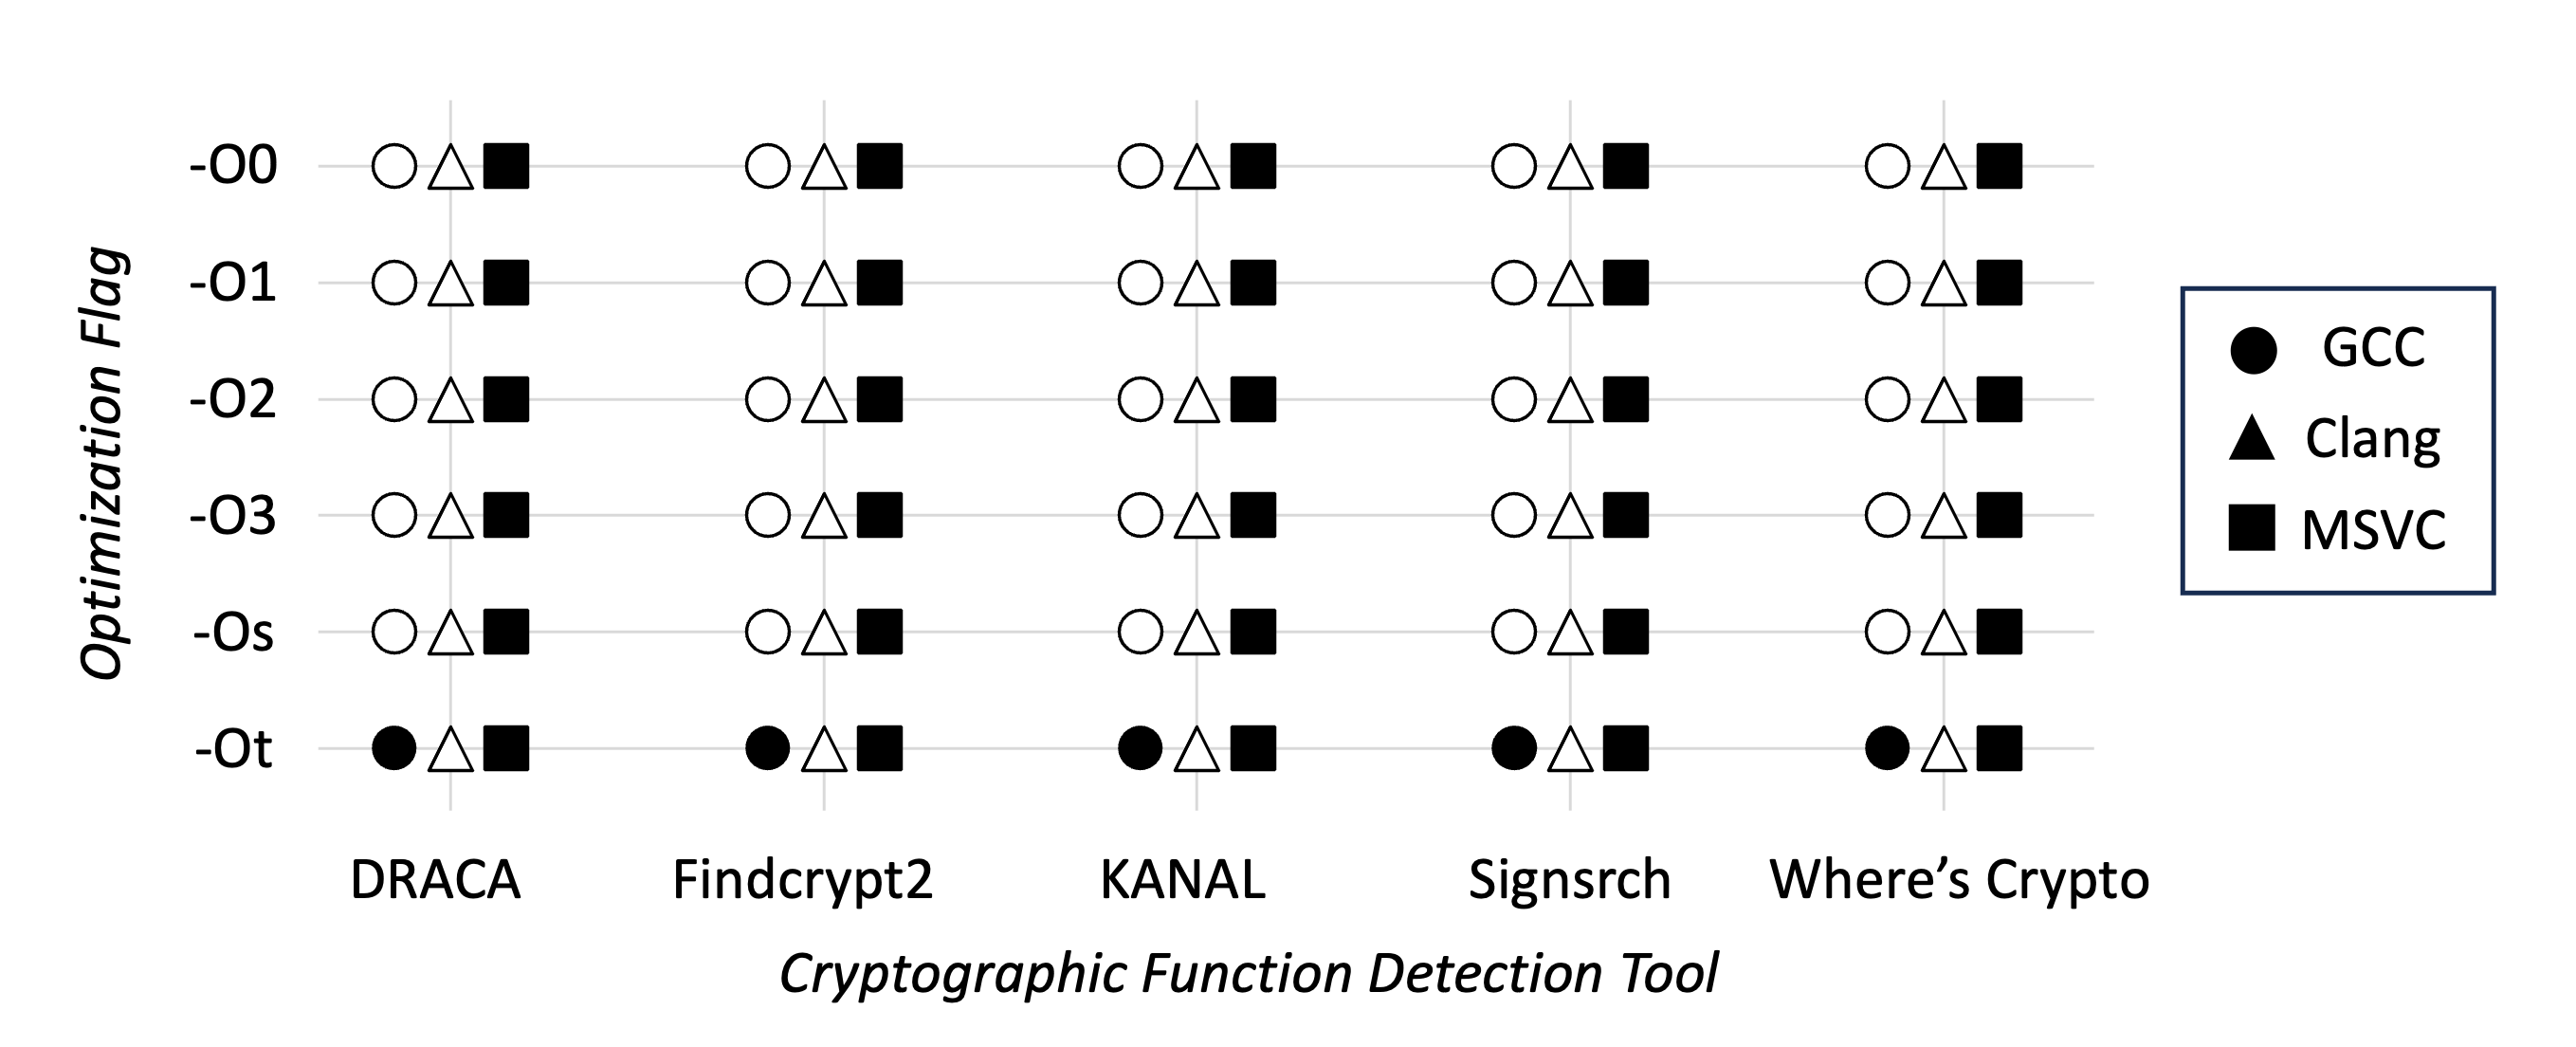
\includegraphics[width=0.8\linewidth,keepaspectratio]{ch-cryptobinary/figure/evaluate_compiler_new.png}
	%\vspace*{-10pt}
  \caption{Evaluation result for MD5 with different compilers. A full marker indicates that function can be detected and an empty marker that it cannot.}
  \label{fig:cryptobinary-evaluate_compiler}
\end{figure}

\fanyo{fix typo in figure!!!}

In this example, DRACA, Findcrypt2, PEiD KANAL, Signsrch, and Where's Crypto support detecting the MD5 algorithm. However, their detection capabilities are influenced by the compiler used. All of these tools can detect the MD5 algorithm in binaries compiled with the MSVC compiler, regardless of the optimization flag. In contrast, for binaries compiled with GCC, they can only detect the MD5 algorithm when the -O0 optimization flag is applied. Furthermore, when using the Clang compiler, none of these tools were able to detect the MD5 algorithm in the binary. This suggests that differences between compilers may significantly impact a tool's analysis results. In general, we found that the MSVC compiler has less impact on detection results compared to GCC and CLANG. Specifically, if a tool can detect a certain cryptographic algorithm in a program compiled by GCC or CLANG, it will also be able to detect that algorithm in the same program compiled by MSVC.

For example, Signsrch shows inconsistent performance with Clang, GCC, and MSVC, identifying the SHA-1 hash function in certain programs compiled with identical optimization flags but using a different compiler. We also observe same behaviour for DARACA when detect XXTEA algorithm (see Table \ref{tab:cryptobinary-benchmarks} for details).

The structure of binaries produced by different compilers, such as MSVC, GCC, and LLVM, can vary significantly due to differences in object file formats, optimization strategies, and code generation techniques. Binary analysis often relies on symbolic information, padding, and inlined data, all of which are heavily influenced by the compiler version~\cite{andriesse2017compiler}. These variations can hinder the effectiveness of cryptographic function detection tools, potentially leading to inaccurate or incomplete detection results.

%\noindent\fbox{%
    %\parbox{\textwidth}{%
        %Future Research Question: At present, it is notable that none of the cryptographic function detection tools take into account the influence of the compiler. Our evaluation results have revealed that the choice of compiler plays a pivotal role in cryptographic function analysis.
        %%We have identified differences in behavior between standard, widely used compilers like GCC and CLANG. Additionally, other non-standard compilers may introduce even more variations and challenges for cryptographic function detection tools. 
        %The exploration of compiler effects and their incorporation into cryptographic function detection tools represents an enticing avenue for future research, and understanding and accounting for these compiler-related influences could significantly enhance the accuracy and reliability.
    %}%
%}

\begin{takeaway}
\textbf{Future Research:} At present, it is notable that none of the cryptographic function detection tools consider the impact of the compiler. Our evaluation results have revealed that the choice of compiler plays a pivotal role in cryptographic function analysis.
        %We have identified differences in behavior between standard, widely used compilers like GCC and CLANG. Additionally, other non-standard compilers may introduce even more variations and challenges for cryptographic function detection tools. 
        The exploration of compiler effects and their incorporation into cryptographic function detection tools represents an enticing avenue for future research.
        Moreover, understanding and accommodating these compiler-related influences could significantly enhance both accuracy and reliability.
        %and understanding and accounting for these compiler-related influences could significantly enhance accuracy and reliability.
\end{takeaway}


% \begin{table}[h]
% \centering
% \begin{tabular}{|cc|c|c|c|c|}
% \hline
% \multicolumn{2}{|c|}{Binary Prog}                    & DRACA  & Findcrypt2 & PEiD KANAL & Where's Crypto \\ \hline
% \multicolumn{1}{|c|}{\multirow{2}{*}{XXTEA}} & gcc   & \cellcolor{gray!25}\cmark & \cmark     & \cmark     & \cmark         \\ \cline{2-6} 
% \multicolumn{1}{|c|}{}                       & clang & \cellcolor{gray!25}\xmark & \cmark     & \cmark     & \cmark         \\ \hline
% \multicolumn{1}{|c|}{\multirow{2}{*}{MD5}}   & gcc   & \cellcolor{gray!25}\cmark & \cellcolor{gray!25}\cmark     & \cellcolor{gray!25}\cmark     & \cellcolor{gray!25}\cmark         \\ \cline{2-6} 
% \multicolumn{1}{|c|}{}                       & clang & \cellcolor{gray!25}\xmark & \cellcolor{gray!25}\xmark     & \cellcolor{gray!25}\xmark     & \cellcolor{gray!25}\xmark         \\ \hline
% \end{tabular}
% \caption{Untitled}
% \label{tab:evaluate_compiler}
% \end{table}

 %\begin{table}[h]
 %\centering
 %\begin{tabular}{|c|c|c|c|c|c|c|c|c|c|c|c|c|}
 %\hline
 %Flag   & None  & -O0   & -O1   & -O2   & -O3   & -Os   & -Ofast & obs\_sub & obs\_fla & obs\_bcf & Multi\_flag 1 & Multi\_flag 2 \\ \hline
 %Prog 1 & \cmark & \cmark & \cmark & \xmark & \xmark & \xmark & \xmark  & \cmark    & \cmark    & \cmark    & \cmark         & \xmark         \\ \hline
 %Prog 2 & \cmark & \cmark & \xmark & \xmark & \xmark & \xmark & \xmark  & \cellcolor{gray!25} & \cellcolor{gray!25} & \cellcolor{gray!25} & \cellcolor{gray!25} & \cellcolor{gray!25} \\ \hline
 %\end{tabular}
 %\caption{Untitled}
 %\label{tab:evaluate_flag}
 %\end{table}

\subsection{Impact of Optimization Flags}
%\emph{R2: Is there any impact from optimization flags?}

Optimization flags and obfuscation can significantly impact the analysis results for cryptographic functions \cite{ren2021unleashing}. CryptoHunt\cite{xu2017cryptographic} and FALKE-MC \cite{aigner2018falke} have explored this direction. CryptoHunt primarily focuses on specific optimization flags such as \texttt{-O0}, \texttt{-O1}, and \texttt{-O2}, while FALKE-MC includes programs compiled with \texttt{-Os} and \texttt{-Ofast} for training. However, we are unable to run either of these tools, so we cannot confirm their detection performance with optimization/obfuscations flags. In order to comprehensively investigate this topic, we have expanded our study to include additional optimization flags, obfuscation techniques, and their combinations, thereby providing a more thorough exploration of their impact on cryptographic algorithm detection.

Our findings indicate that both optimization flags and obfuscations can affect detection capability. For instance, based on our results in \autoref{tab:cryptobinary-benchmarks}, we can see that Findcrypt2, PEiD KANAL, Signsrch, and Where's Crypto can detect MD5 when compiled without optimization/obfuscation flags or compiled with \texttt{-O1}. However, none of these tools can detect MD5 if the binary program is compiled with advanced optimization/obfuscation flags such as \texttt{-O2}, \texttt{-Ofast}, or \texttt{-obs\_sub}. In addition, we observed that Signsrch exhibits inconsistent performance for SHA-1 or SHA-256, and DRACA shows unstable performance with XTEA and XXTEA when running with optimization or obfuscation flags.
Optimization flags significantly alter the structure and behavior of a binary program by improving performance, reducing size, and modifying control flow. Techniques like function inlining, loop unrolling, and dead code elimination obscure the original source code structure, making it more difficult for analysts to identify cryptographic functions.
% Table \ref{tab:evaluate_flag} shows selected evaluation results of Signsrch with two different experiment. Experiment 1 is a program contains the SHA-1 hash function compiled by CLANG with different optimization flags or obfuscations, while experiment 2 contains the MD5 hash function compiled by GCC with different optimization flags (as the GCC compiler does not support obfuscations).

% \begin{table}[h]
% \vspace*{-6pt}
% \centering
% \footnotesize
% \begin{tabular}{|c||c|c|c|}
% \hline
% Flag          & SHA-1        & MD5                 \\ \hline \hline
% None          & \cmark       & \cmark              \\ \hline
% -O0           & \cmark       & \cmark              \\ \hline
% -O1           & \cmark       & \xmark              \\ \hline
% -O2           & \xmark       & \xmark              \\ \hline
% -O3           & \xmark       & \xmark              \\ \hline
% -Os           & \xmark       & \xmark              \\ \hline
% -Ofast        & \xmark       & \xmark              \\ \hline
% obs\_sub      & \cmark       & \cellcolor{gray!25} \\ \hline
% obs\_fla      & \cmark       & \cellcolor{gray!25} \\ \hline
% obs\_bcf      & \cmark       & \cellcolor{gray!25} \\ \hline
% -obs\_sub, obs\_fla, obs\_bcf & \cmark       & \cellcolor{gray!25} \\ \hline
% -obs\_sub, obs\_fla, obs\_bcf, -O3 & \xmark       & \cellcolor{gray!25} \\ \hline
% \end{tabular}
% %}
% \caption{Evaluation results of Signsrch with different optimization flags}
% \label{tab:evaluate_flag}
% \vspace*{-0.6cm}
% \end{table}

% We discovered that both optimization flags and obfuscations can affect detection, potentially resulting in false negatives (where the binary contains a cryptographic algorithm but the tool cannot detect it). For example, Signsrch successfully detects TEA in Program 1 compiled without any optimization flags or obfuscations. However, with additional optimization flags, Signsrch cannot detect any cryptographic algorithms at all anymore, resulting in false negatives.

% Meanwhile, Signsrch successfully detects MD5 in Program 2 compiled with no optimization flags or -O0, but cannot detect MD5 in the binary compiled with any other optimization flags or obfuscations. We observed the same results when detecting MD5 with other tools. Therefore, we conclude that current cryptographic detection tools may not be able to handle some algorithms, like MD5, if the binary is compiled with advanced optimization flags such as $-O3$.

%\noindent\fbox{%
    %\parbox{\textwidth}{%
        %Future Research Question: Optimization and obfuscation have been noticed by some researchers such as CryptoHunt, a cryptographic detection tool designed for obfuscated binaries. However, the limitation of CryptoHunt, such as slow time performace due to the large trace size, may reduce its applicability such as large scale project.  Given that certain other tools struggle to handle obfuscated binaries in certain algorithms,  we maintain that the exploration of optimization and obfuscation remains an interesting and important future research direction.
    %}%
%}

\begin{takeaway}
\textbf{Future Research:} The effects of optimization and obfuscation have been noted in works such as CryptoHunt, which is designed specifically for obfuscated binaries. However, limitations such as slow performance due to the large trace size, may reduce its applicability for large scale projects. Considering that many tools seem to face challenges with obfuscated binaries, we assert that investigating the effects of optimization and obfuscation continues to be a compelling and critical avenue for future research.
\end{takeaway}

% \begin{figure}
% \centering
% \begin{minipage}{.45\textwidth}
%   \centering
%   \includegraphics[width=\linewidth]{./images/evaluate_algo.jpg}
%   \caption{Untitled}
%   \label{fig:evaluate_algo}
% \end{minipage}%
% \qquad
% \begin{minipage}{.45\textwidth}
%   \centering
%   \includegraphics[width=1.15\linewidth]{./images/evaluate_tool.jpg}
%   \caption{Untitled}
%   \label{fig:evaluate_tool}
% \end{minipage}
% \end{figure}

\subsection{Impact of Different Algorithm Versions}
\label{subsec:cryptobinary-algo-version}
% \begin{figure}[ht]
%   \includegraphics[width=\columnwidth,keepaspectratio]{./images/evaluate_nonstandard.jpg}
%   \caption{Untitled}
%   \label{fig:evaluate_nonstandard}
  
% \end{figure}

%\emph{R5: Is the version of the algorithm significant during detection?}

We also carried out evaluations to determine whether variations in a cryptographic algorithm affects the success of its detection. As a case study, we analyzed different variants of the Tiny Encryption Algorithm (TEA), including standard TEA, XTEA, and XXTEA. While all the tools were able to successfully detect TEA binaries with any of these three variants, we observed some interesting details in the detection results.

\begin{table}[h]
%\vspace{-6pt}
\centering
\begin{tabular}{l||l|l}
\hline
Algorithm & DRACA                                                                      & Signsrch                                                                                   \\ \hline \hline
TEA   & \begin{tabular}[c]{@{}l@{}}* RC5 or RC6 - 50\%\\ ** TEA - 67\%\end{tabular} & \begin{tabular}[c]{@{}l@{}}* TEA1\_DS {[}32.le.4{]}\\ ** TEA encryption/decryption\end{tabular} \\ \hline
XTEA  & \begin{tabular}[c]{@{}l@{}}* RC5 or RC6 - 50\%\\ ** TEA - 34\%\end{tabular} & * TEA1\_DS {[}32.le.4{]}                                                                     \\ \hline
XXTEA & \begin{tabular}[c]{@{}l@{}}* RC5 or RC6 - 50\%\\ ** TEA - 67\%\end{tabular} & * TEA1\_DS {[}32.le.4{]}                                                                     \\ \hline
\end{tabular}
%}
\caption{Output when evaluating DRACA and Signsrch with different variants of TEA}
\label{tab:cryptobinary-evaluate_variant}
%\vspace*{-0.7cm}
\end{table}

For example, as shown in Table \ref{tab:cryptobinary-evaluate_variant}, when using DRACA to analyze binaries containing TEA or XXTEA, the tool provides a confidence score. It tends to determine that a binary program is more likely to contain TEA functions if TEA or XXTEA is present. However, when analyzing binary programs containing XTEA, DRACA may incorrectly identify RC5 or RC6 as being present in 50\% of cases, and TEA functions in only 34\% of cases. In contrast, Signsrch is able to detect TEA functions in all three binary programs containing TEA, XTEA, or XXTEA, but it may identify different TEA signatures in each binary.

%\noindent\fbox{%
    %\parbox{\textwidth}{%
        %Future Research Question: Our evaluations suggests that the variant versions of cryptographic algorithms also play a crucial role in detection, and that cryptographic function detection tools may not be able to accurately detect certain variant algorithms based on their signatures alone. Currently, there is no approach focuses on this difference, which could be a future research path for crytpographic function detection.
    %}%
%}

\begin{takeaway}
\textbf{Future Research:} Our evaluations indicates that the variant or version of a cryptographic algorithm plays a crucial role in its detection, suggesting that existing tools might struggle to accurately identify certain variants based on their signatures alone. Currently, there is no approach that focuses on this difference, which could be an interesting future research path.
\end{takeaway}



\subsection{Impact of Intentional Evasion Tactics}
%\fanyo{Change title to Detect binary with malware or something similar?}
\label{subsec:cryptobinary-algo-version1}
%\emph{R6: Are ``malicious'' versions of cryptographic algorithms trickier to detect?}

We selected multiple (ransomware) malware binaries, including CryptoLocker \cite{hansberry2014cryptolocker}, CryptoWall \cite{cabaj2015network}, Locky \cite{locky}, TeslaCrypt \cite{lemmou2018infection}, and Win32Dircrypt \cite{win32dircrypt}, to evaluate if cryptographic detection tools are better or worse at finding cryptographic algorithms in malware binaries (where authors might intentionally try to obfuscate the presence of cryptography) versus normal applications. 

%The CryptoLocker ransomware is a trojan that targeted computers running Microsoft Windows via infected email attachments and encrypted certain types of files stored on local and mounted network drives. 
%Cryptowall operates as a ransomware virus that employs a Trojan horse to encrypt files on a compromised computer, demanding users to make a payment in exchange for a decryption key.
%Locky is ransomware malware that delivers malicious macros through Microsoft Word documents attached to emails.
%TeslaCrypt is a ransomware trojan that targets game-play data, with newer variants also affecting other file types \cite{GALLAGHER_2015}.  
%Win32Dircrypt may encrypt file through spam emails or by being downloaded by other malware and ask payment for decryption.

We tested the tools with these malware samples and present the results in Table \ref{tab:cryptobinary-evaluate_malware}. It is worth noting that malware may have different versions depending on the discovery date, and detection results are highly dependent on these versions. We found that the tools could detect cryptographic functions in TeslaCrypt version 2 but failed to do so in versions 1 and 3. This suggests that the malware may employ non-standard algorithms to evade binary analysis in certain versions, increasing the difficulty of detection. Furthermore, cryptographic functions in CryptoLocker's September 10, 2013 version were detectable by the tools, but in the November 20, 2013, and January 22, 2014 versions, they were no longer detectable. In the latter two versions, some tools identified the presence of anti-debugging techniques in the malware, which might explain why cryptographic functions could not be detected anymore.

%We found that none of the cryptographic detection tools we chose can detect AES in CryptoWall, since CryptoWall primarily uses RSA, and may only use non-standard versions of AES in its source code.
%Meanwhile, most tools cannot detect AES in TeslaCrypt, but DRACA successfully finds AES algorithm in TeslaCrypt version 3372C.  And even though AES cannot be detected, some tools still successfully found other cryptographic hash algorithms in CryptoWall and TeslaCrypt including SHA256, RIPEMD, and Fork256.


\begin{table}[h]
\vspace*{-0.1cm}
\centering
\begin{adjustbox}{max width=\textwidth}
\begin{tabular}{c||c|c|c|c}
\hline
Malware                 & DRACA  & PEiD KANAL  & Signsrch  & Note       \\ \hline 
\hline
CryptoLocker\_10Sep2013 & \xmark & \cmark      & \cmark    &            \\ \hline
CryptoLocker\_20Nov2013 & \xmark & \xmark      & \xmark    & anti-debug \\ \hline
CryptoLocker\_22Jan2014 & \xmark & \xmark      & \xmark    & anti-debug \\ \hline
CryptoWall              & \xmark & \xmark      & \xmark    & anti-debug \\ \hline
Locky                   & \xmark & \xmark      & \xmark    &            \\ \hline
TeslaCrypt\_v1          & \xmark & \xmark      & \xmark    &            \\ \hline
TeslaCrypt\_v2          & \cmark & \cmark      & \cmark    &            \\ \hline
TeslaCrypt\_v3          & \xmark & \xmark      & \xmark    &            \\ \hline
Win32Dircrypt           & \xmark & \cmark      & \cmark    &            \\ \hline
\end{tabular}
%}
\end{adjustbox}
\caption{Evaluation results for cryptographic function detection in different malware versions}
\label{tab:cryptobinary-evaluate_malware}
%\vspace*{-0.6cm}
\end{table}


% \begin{table}[]
% \vspace*{-0.1cm}
% \centering
% \begin{tabular}{|l|c|c|c|}
% \hline
% Malware & DRACA & PEiD KANAL & Signsrch \\ \hline
% CryptoWall\_1002 & \Circle & \LEFTcircle & \Circle   \\ \hline
% CryptoWall\_1003 & \Circle & \LEFTcircle & \Circle \\ \hline
% TeslaCrypt\_3372C & \CIRCLE & \LEFTcircle & \LEFTcircle \\ \hline
% TeslaCrypt\_51B4E & \Circle & \Circle & \Circle \\ \hline
% TeslaCrypt\_E906F & \Circle & \Circle & \Circle \\ \hline
% \end{tabular}
% \caption{Evaluation results for different malware versions}
% \label{tab:evaluate_malware}
% \vspace*{-0.6cm}
% \end{table}

%\noindent\fbox{%
    %\parbox{\textwidth}{%
        %Future Research Question: Malware detection is a major application for cryptographic function detection, and based on our evaluation, current cryptographic detection tool may not be able to detect the crytpographic function in the malware. Other researcher also notice this issues, and for example, environment-sensitive malware is a threat to CryptoHunt, which may result in false negative. Therefore, cryptographic function detection in malware sould be a major future developement for this topic.
    %}%
%}

\begin{takeaway}
\textbf{Future Research:} Cryptographic function detection can be a useful component in identifying malware, and according to our investigation, current tools do not consistently detect cryptographic functions within the malware samples.  This challenge has been noted in other research as well, for example, CryptoHunt identified environment-sensitive malware as a potential source of false negatives in detection efforts. Therefore, cryptographic function detection primarily focused on targeting malware could be a highly relevant source of future research in this area.
\end{takeaway}

% \subsection{Other Evaluations}
% A single binary program may contain multiple cryptographic algorithms that can be detected by the tool. When testing DRACA with a TEA program without obfuscation, the tool identified multiple cryptographic algorithms. Specifically, DRACA detected 67\% of TEA, 50\% of RC5/RC6, and 23\% of SHA-1. Furthermore, Signsrch was able to recognize the bzip2 binary due to the specific signature that Signsrch supports.



%%%%%%%%%%%%%%%%%%%%
\section{Discussion}
\label{sec:cryptobinary-discussion}

We now provide a discussion backed by our evaluation results and examination of existing work and implemented tools, delving into broader issues that we discovered.  This includes discussing additional overarching future research directions and key areas where improvements can be made moving forward.

%Within this particular section, we aim to delve deeper into the issues and potential avenues for further research that we have identified based on our comprehensive evaluation results. With consideration of the evaluation results, we found our some issues to detect cryptographic function in binary. Meanwhile, we have discovered several key areas where improvements could be made.


\subsection{Approaches to Algorithm Detection in Tools}

%\emph{R4: Can the same tool perform similarly well across different algorithms?}
% \begin{figure}[h]
%   \includegraphics[width=0.5\linewidth,keepaspectratio]{./images/evaluate_tool.jpg}
%   \caption{Untitled}
%   \label{fig:evaluate_tool}
  
% \end{figure}

We start by discussing the detection results of a single tool for different algorithms. We opted to evaluate 12 distinct algorithms (AES, DES, ECC, MD5, RC4, RC5, RSA, SHA-1, SHA-256, TEA, XTEA, and XXTEA) along with our microbenchmarks, various libraries, and a large-scale project.

Based on our evaluation (see \autoref{tab:cryptobinary-benchmarks}), we found that PEiD KANAL, SignSrch, and Where's Crypto can detect most algorithms we selected. This was somewhat expected as Where's Crypto is a more modern detection tool. HCD demonstrated average performance in our evaluation results.
%but it is the only tool that can detect ECC. 
Nonetheless, we came across cases where tools did not detect cryptographic functions they were expected to identify, indicating potential need to enhance detection accuracy.

\begin{takeaway}
\textbf{Future Research:} Current tools seemingly employ various (often distinct) approaches compared to one another. Many of these tools also provide developers with the opportunity to expand and enhance their detection capabilities. Therefore, future research could focus on improving existing technologies within individual tools and existing approaches to achieve broader applicability with higher detection rates, and to make it so that users do not need to use different tools to best identify different algorithms.
\end{takeaway}

\subsection{AI/ML Approach}
Artificial intelligence and machine learning (AI/ML) have been extensively applied across various domains to address complex problems. Previous works, like CryptoKnight, have utilized machine learning techniques for cryptographic function detection. However, in our evaluation, we found that these tools did not exhibit satisfactory performance. We attribute this issue not to the approach itself, but rather to the fact that these tools typically only offer a demonstration to showcase the potential application of AI/ML in this field. The main problem lies in the lack of sufficient signatures or analysis provided by these tools, which is likely the primary reason for their low performance.
\begin{takeaway}
\textbf{Future Research:} 
While current AI/ML based tools demonstrate the feasibility of utilizing AI/ML in cryptographic function detection, they fall short in providing the robust and comprehensive signature or analysis capabilities necessary for accurate detection.  These seem like promising future research directions.
\end{takeaway}

\subsection{Lack of Support for Modern Cryptographic Algorithms}

Many modern cryptographic algorithms, such as general Elliptic-Curve Cryptography (ECC) and more specifically ECDSA and ECDHE, have found widespread use in diverse applications~\cite{harkanson2017applications} due to their advantages in terms of smaller private key size and improved efficiency at equivalent or higher security levels. ECDSA is utilized in a number of areas, including electronic healthcare, banking, commerce, and vehicles \cite{al2019efficient}, and is currently supported by most major libraries, including cryptlib, Crypto++, libgcrypt, LibreSSL, and OpenSSL.
However, our evaluation reveals that existing work lacks the ability to find such modern algorithms. As such, this could be a rich area for future development and improvement. 
\begin{takeaway}
\textbf{Future Research:} 
As the prevalence of applications adopting ECC continues to rise, the ongoing development of cryptographic function detection has led to a disconnect between the outcomes of these efforts and the real-world applications that people are eager to test, leading to an important direction for future research.
\end{takeaway}

% Besides the evaluation metrics we evaluated in Section \ref{subsec:metrics} The false positive may affected by the 
% This underscores the importance of recognizing that the implementation of cryptographic functions can significantly impact detection ability. The presence of optimizations or deviations from the standard algorithm can also lead to false negatives in the detection process.
\subsection{Comparative Detection of Similar Algorithms Across Various Tools}
% \begin{figure}[h!]
%   \includegraphics[width=0.5\linewidth,keepaspectratio]{./images/evaluate_algo.jpg}
%   \caption{Untitled}
%   \label{fig:evaluate_algo}
%\emph{R3: Are some algorithms easier to detect compared to others?}

% \end{figure}
Our evaluation helps provides insights from an algorithmic perspective on how well different tools can detect the same cryptographic algorithm. In our evaluation, we test the tools' abilities to find cryptographic functions in different settings (optimization flags, compilers, etc.). \autoref{fig:cryptobinary-algo_easy} shows the percentage of algorithms that can be successfully detected by a tool across all evaluation experiments that we ran.
We can see that TEA, RC5, and SHA can be successfully detected in most experiments. However, AES, and MD5 can only be found in a few experiments, with algorithms like RC4 and ECC not even being detected at all.

\begin{figure}[t]
    \centering
  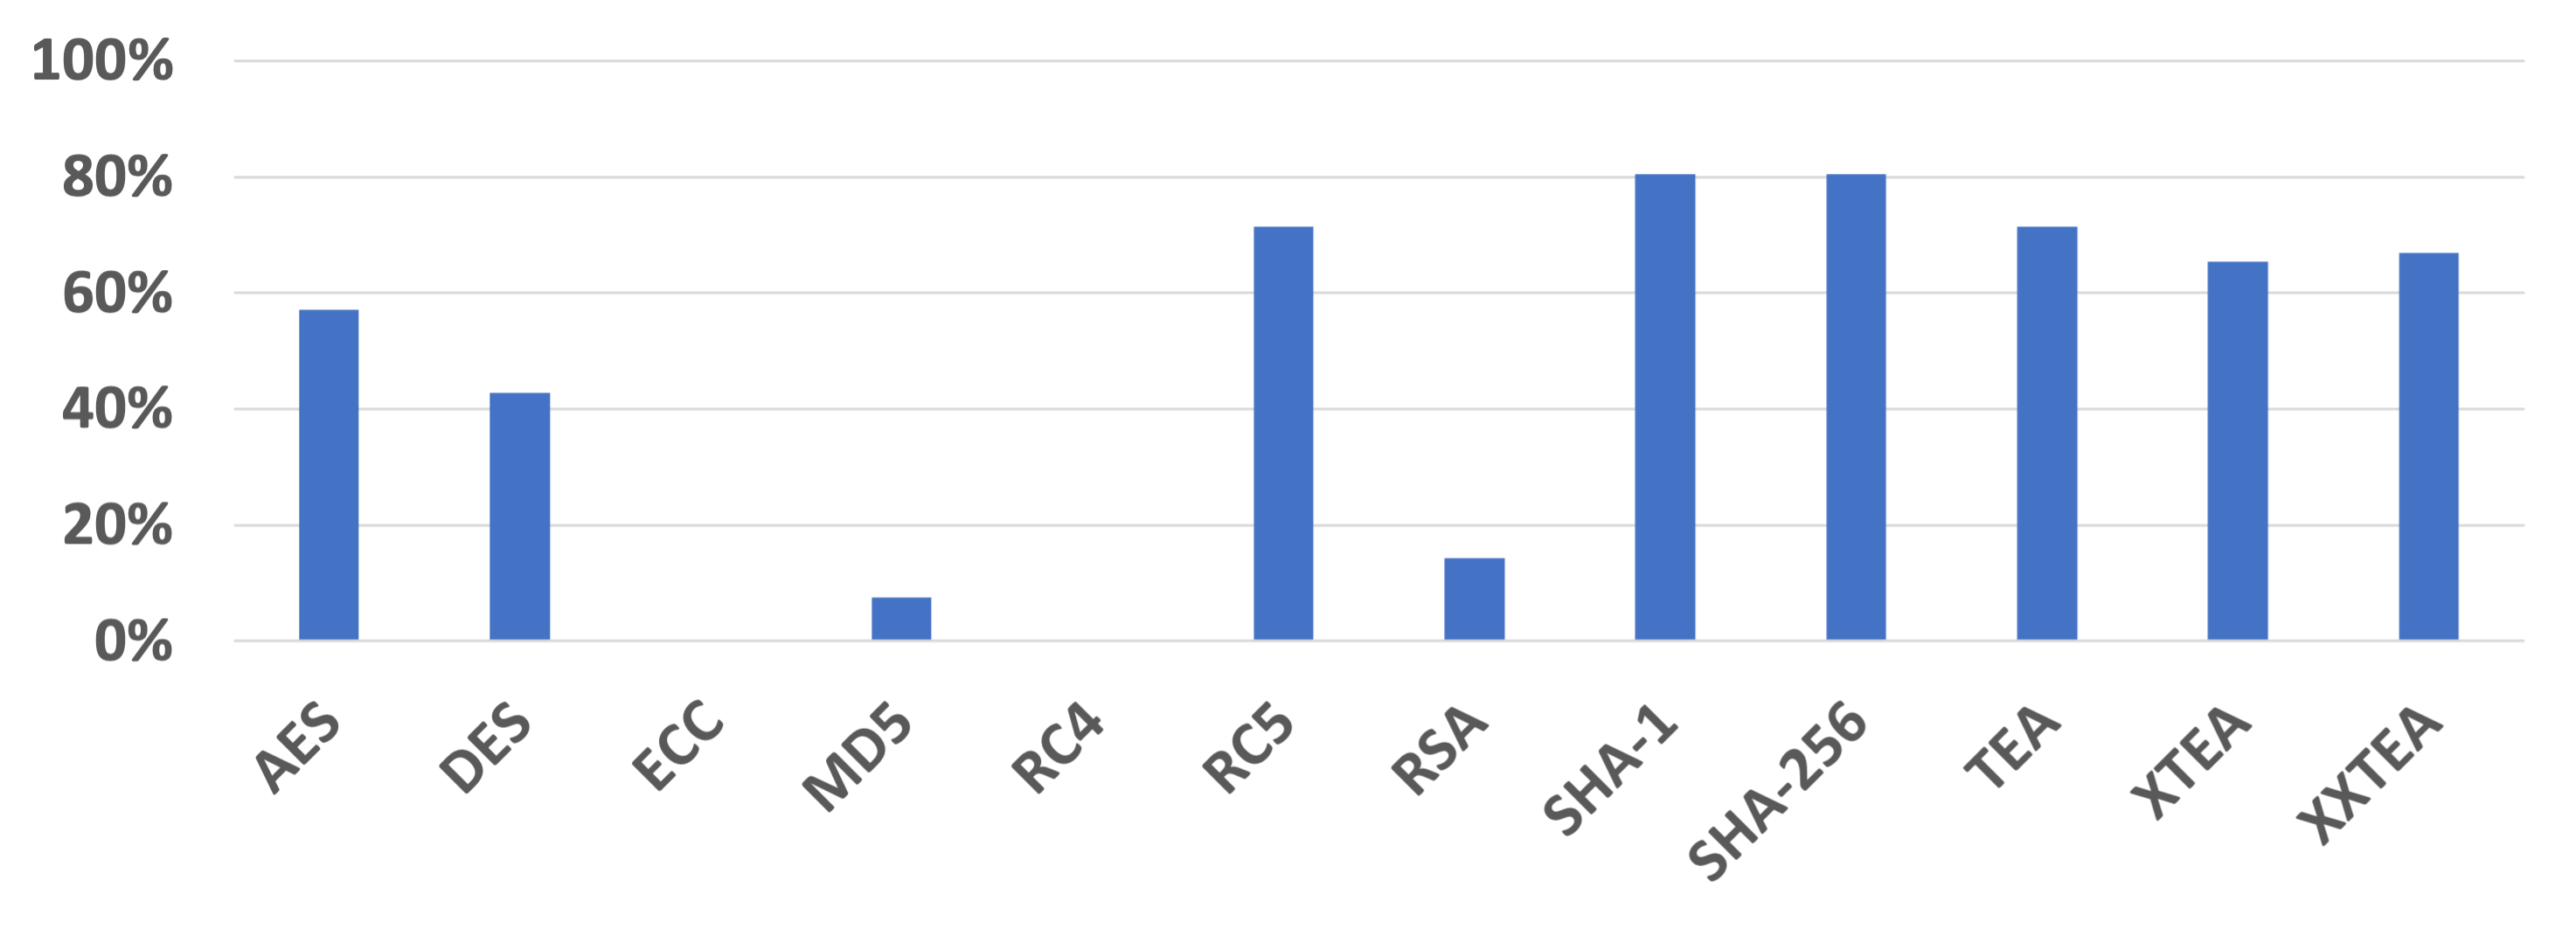
\includegraphics[width=0.95\linewidth,keepaspectratio]{ch-cryptobinary/figure/algoeasy.png}
  \caption{Detection percentage by algorithm across all tools}
  \label{fig:cryptobinary-algo_easy}
\end{figure}

From our observations, it is not evident that there exists a consistent rule governing the ease of detecting specific categories of cryptographic functions. For instance, when considering two hash functions, MD5 and SHA, we note markedly different results. Even within the same family we find variations; TEA and RC5, both belonging to the block cipher family, exhibit detectability, while DES, another block cipher, proves more challenging to detect.

%\noindent\fbox{%
    %\parbox{\textwidth}{%
        %Future Research Question: Some cryptographic algorithms are more challenging to detect than others, as indicated by our evaluation results. Notably, we have not observed a distinct pattern suggesting that algorithms within a specific category consistently present greater difficulty in detection. Therefore, the future research could focus on how to detect cryptographic algorithms that appear to be harder to identify or investigate the underlying factors that contribute to variations in the detectability of algorithms within the same category.
    %}%
%}

\begin{takeaway}
\textbf{Future Research:} Some cryptographic algorithms appear to be more challenging to detect than others. However, we have not observed a distinct pattern suggesting that algorithms within a specific category consistently present greater difficulty in detection. Therefore, future research could focus on how to detect cryptographic algorithms that appear to be harder to identify or investigate the underlying factors that contribute to variations in the detectability of algorithms within the same class.
\end{takeaway}



%\subsection{Leveraging General Binary Analysis Techniques}
%\label{leverage-binary}
%%\noindent\fbox{%
    %%\parbox{\textwidth}{%
        %%Future Research Question: 
    %%}%
%%}
%Binary code similarity analysis is an active area of research in the software community. There has been a plethora of research~\cite{david2017similarity, saebjornsen2014detecting, liu2018eclone, chandramohan2016bingo, mckee2019software, ding2019asm2vec, ming2017binsim, xu2017neural} to compare two or more binaries to identify their similarities or variances.  
%
%BLEX~\cite{egele2014blanket} proposed a dynamic similarity testing system based on the novel technique of blanket execution 
%consisting of seven binary code semantics extractor. Tinbergen~\cite{mckee2019software} presented a framework which infers function semantics through program state change. DyCLINK~\cite{su2016code} used dynamic dependency graph to capture code behavior at the instruction level and then
%performed similarity analysis via computing an isomorphism between sub graphs.
%There are also some notable NLP based binary similarity analysis techniques~\cite{ding2019asm2vec, xu2017neural}.
%Asm2Vec~\cite{ding2019asm2vec} is a representation learning model that learns latent lexical semantics between
%tokens and represents an assembly function as an internally weighted mixture of collective semantics.
%Gemini~\cite{xu2017neural} proposes a neural network-based approach to compute the embedding, i.e., a numeric vector, based on the control
%flow graph of each binary function and then performs the similarity detection via measuring the distance between the embeddings for two functions.

%\begin{takeaway}
%\textbf{Future Research:}
%Although binary similarity research is very similar to some cryptographic function identification approaches and shares a similar set of challenges, cryptographic detection research has a much more limited scope of work and techniques thus far.
%Hence, an avenue for future research is investigating the use of binary similarity techniques in this more targeted space.  
%\end{takeaway}


% \subsection{Discussion of Evaluation Results}
% Based on our evaluation, we found that most of the cryptographic detection tools have similar performance such as

% \begin{itemize}[leftmargin=*]
%     \setlength{\itemsep}{0pt}
%     \setlength{\parskip}{0pt}
%         \item Cannot detect RSA and modern cryptohtrapicy algorithm ECC in binary
%         \item Optimization flag and compiler do not affect the detetcion results in SHA (except for Signsrch) and TEA
%         \item Can only detect MD5 compiled with no flag or $\O0$ in GCC
% \end{itemize}

% In the course of our evaluation, we have encountered instances of false negatives in certain cryptographic detection tools. For instance, both DRACA and FindCrypt2 assert their ability to detect DES functions within binaries. However, we were unable to replicate this result even when using a standard DES implementation without any obfuscation during compilation.

\subsection{User Experience}

Considering the experience and insights we have garnered from our evaluation process, we believe that discussing the developer experience is also an intriguing topic, in terms of how developers interact with these tools and their ease of use.

Older cryptographic detection tools, such as DRACA, PEiD KANAL, and SignSrch, do not require developers to compile and build the tools from source code. Developers can readily utilize these tools with supported operating systems. However, when compared to some better performing tools, these user-friendly alternatives exhibit lower performance and utility. For example, obfuscation can disturb the binary analysis process of Signsrch, leading to false negatives in the detection of certain cryptographic algorithms. Furthermore, DRACA struggles to accurately analyze packed executable programs, and consequently, it can only provide a rudimentary analysis outcome, despite its ease of use.

In addition to the aforementioned challenges, some tools pose difficulties for users due to technological complexity or data-related issues. Take, for instance, IDA Scope, Findcrypt2, and Where's Crypto, which all rely on IDA Pro. IDA Pro is not a free, open-source software, and these tools cannot be utilized by developers without it. Conversely, tools such as CryptoKnight and other machine learning-based techniques require users to provide substantial amounts of data, which further compounds the difficulty of using these tools. 

However, these tools generally exhibit superior performance when compared to user-friendly alternatives. For instance, CryptoHunt consistently yields accurate analysis results for identification within obfuscated programs. Where's Crypto, one of the most recent cryptographic detection tools, broadens the scope of analysis to encompass unfamiliar and proprietary cryptographic primitives, without relying on heuristics to select code fragments.

\subsection{Challenges for Future Research}
\label{subsec:cryptobinary-challenges}

%Identifying cryptographic functions has its own sets of challenges. 
Based on our evaluation, we have identified several challenges that make cryptographic function identification difficult.
In this subsection, we discuss some of these challenges, as we believe they may help inform future tool development and areas of research.

%%%%%%%%%%%%%%%%%%%%%%%%
\parhead{Obfuscation.} One of the major challenges in cryptographic function identification is obfuscation.
The initial purpose of obfuscation was to protect software intellectual
property~\cite{collberg1997taxonomy} from malicious reverse engineering
attempts. However, malware authors adopted obfuscation techniques as a way to
avoid detection. Various types of obfuscation techniques have been implemented
to thwart any form of detection. These obfuscation techniques can be primarily
categorized as: control-flow obfuscation, data obfuscation, and layout obfuscation.
For a variety of reasons, one might still wish to identify cryptographic code
even in the face of such obfuscation techniques, particularly given its prevalence nowadays.
%Malware authors mostly adhere to control-flow and data obfuscations.

Control-flow obfuscation is the most common type of obfuscation. A control-flow graph (CFG) \cite{CFG} embodies the graphical
representation of the flow of a program. To hinder CFG-based detection, malware authors introduce techniques such as including bogus control-flow \cite{li2021code}, control-flow flattening \cite{cfg_f}, and opaque predicates \cite{xu2018opaque}. 
Similar to control flow obfuscation, data obfuscation techniques, like data aggregation and data
splitting, attempt to hinder approaches based on input/output relationships. For example, one might split a single variable into two to prevent detection.
%\autoref{lst:data_splitting} shows an example of data
%obfuscation, and how one variable used in \autoref{lst:normal_program}
%can be split into two variables to prevent detection.  
%
%\lstset{language=C,
        %label=lst:normal_program,
        %float=h,
        %caption={Normal program},
        %captionpos=b,
        %showlines=true,
        %breaklines=true,
        %breakatwhitespace=true,
        %tabsize=2,basicstyle=\footnotesize}
%\hspace*{-1.1cm}
%\begin{lstlisting}
%int var1 = func1();
%int var2 = func2();
%
%while(condition statement) {
	%int p1 = var1 * var2;
	%int p2 = var1 + var2;
%}
%\end{lstlisting}%
%%\hfill
%%\hspace*{0.1cm}
%\vspace{5pt}
%
%\lstset{language=C,
        %label=lst:data_splitting,
        %float=h,
        %caption={Data splitting},
        %captionpos=b,
        %breaklines=true,
        %breakatwhitespace=true,
        %tabsize=2,basicstyle=\footnotesize}
%\begin{lstlisting}
%int var1 = func1();
%int var2 = func2();
%
%short var11 = (short) (var1 >> 16);
%short var12 = (short) (var1 & 0xffff);
%
%while(condition statement) {
    %int new_var = (int) ((var11 << 16) | (var12 & 0xffff););
%
    %int p1 = new_var * var2;
    %int p2 = new_var + var2;
%}
%\end{lstlisting}
Layout obfuscation~\cite{xu2020layered} scrambles the layout of a program's instructions while keeping the original syntax intact. Layouts can be obfuscated by adding meaningless classifiers, stripping redundant symbols, separating related code, as well as adding junk code.

%%%%%%%%%%%%%%%%%%%%%%%%%%%%%%%%%%%%%

\parhead{Implementation Variation.} Despite having a well-defined specification, cryptographic algorithms can be implemented in a number of
ways while still achieving the same result.  In addition, cryptography is not always implemented correctly or exactly to spec.
For example, buggy implementations of the TEA algorithm
were found~\cite{calvet2012aligot} in malware such as Storm Worm and Silent Banker.
Hence, even if a detection approach can find an ideal implementation of an algorithm, there is no
guarantee it can also detect all the implementation variations
of the same algorithm. 
%We believe it is valuable (but challenging) to be able to identify both intended implementation variations, as well as as incorrect (but close) ones.
Our evaluations in this space are discussed in \autoref{subsec:cryptobinary-algo-version} and \autoref{subsec:cryptobinary-algo-version1}.

%%%%%%%%%%%%%%%%%%%%%%%%%%%%%%%%%%%%%%%%%%%%%%%%%%%

\parhead{Differences in Cryptographic Functions.} There are fundamental differences in different classes of cryptographic algorithms.
Cryptographic features (see \autoref{sec:cryptobinary-features}) present in one algorithm may not be present in others.
For instance, the data avalanche effect~\cite{li2012cipherxray} which says that an insignificant change in the input parameters can
make significant differences in the output, works well for identifying block ciphers. In the case of stream ciphers, there are
no such observations like data avalanching. Tools must be designed to account for these differences if they wish to identify broad classes of algorithms.

%%%%%%%%%%%%%%%%%%%%%%%%%%%%%%%%%%%%%%%%%%%%%%%%%%%

\parhead{Compilers.} The choice of compiler can significantly impact the binary structure of a program in various ways such as format, linking, inline functions, and compatibility with different architectures. The incorporation of anti-analysis techniques further adds to the complexity of cryptographic function detection. Consequently, working with different compilers can introduce numerous challenges. 
%Possessing knowledge about compiler behavior becomes essential for reverse engineers, security analysts, and detection tools to effectively identify cryptography within a binary program.
Our study (Section \ref{subsec:cryptobinary-effect-compiler}) demonstrates how a tool's detection capabilities can vary greatly depending on the compiler used.


%%%%%%%%%%%%%%%%%%%%%%%%%%%%%%%%%%%%%%%%%%%%%%%%%%%
\parhead{Comparison to General Binary Analysis.}
Binary code similarity analysis is an active area of research in the software community. There has been a plethora of research~\cite{david2017similarity, saebjornsen2014detecting, liu2018eclone, chandramohan2016bingo, mckee2019software, ding2019asm2vec, ming2017binsim, xu2017neural} to compare two or more binaries to identify their similarities or variances.  
While such generic binary analysis techniques can be leveraged in the detection of cryptographic functions, future researchers should bear in mind that detecting cryptographic functions in binary code remains a multifaceted challenge. Cryptographic algorithms exhibit significant variability in terms of complexity and implementation. They often involve intricate mathematical operations and employ various techniques such as bit manipulation, modular arithmetic, and logical operations. This complexity can pose difficulties in identifying cryptographic functions without specific knowledge of the algorithm being utilized.
%Furthermore, unlike some other types of functions or libraries that may have standardized signatures or calling conventions, cryptographic functions may lack easily recognizable patterns or signatures. They can be 
In addition, they can be implemented in diverse ways and may not adhere to consistent naming or calling conventions, rendering them more challenging to identify through static analysis alone.

%Additionally, detecting cryptographic functions in binary code constitutes a specialized domain within general binary analysis. Consequently, we anticipate a higher level of accuracy compared to detecting other types of functions in binary code.


%%Where's crypto, one of the latest cryptographic detection tool developed in 2021, provides an novel approach combines subgraph isomorphism with symbolic execution to find cryptographic algorithm in binary, but we did not discover a major performance improvement according to our evaluation results.


\section{Conclusion}

Cryptographic function identification has been a popular area of study in both academia and industry. However, we noticed a lack of consistent means for evaluation and comparison among tools.
As such, in this work we conduct comprehensive reproduction and replication studies on all existing work in the space.
To complement the traditional R+R studies, we developed a comprehensive testing and evaluation framework which includes a number of modern cryptographic algorithms and real world examples, that allow for the comparison of both existing and future work in a uniform manner.
Finally, we highlight major gaps in existing work, especially as they relate to modern cryptographic primitives and real-world use cases,
and discuss a variety of important avenues for future work.
\chapter{SNARKPROBE: AN AUTOMATED SECURITY ANALYSIS FRAMEWORK FOR ZKSNARK IMPLEMENTATIONS}
\label{ch:snarkprobe}

\textit{This chapter is based on joint work with Christina Garman (Purdue University) along with Yuquan Xu (Purdue University, Georgia Tech) \footnote{This work was supported by NSF grant CNS-2047991.}. The paper was published in proceedings of the 2024 International Conference on Applied Cryptography and Network Security, pages 340-372 \cite{fan2024snarkprobe}.}

\section{Introduction}
\label{sec:snarkprobe-introduction}

We have seen a growing interest in privacy and privacy-enhancing technologies from the general public~\cite{adoption}, which has led to subsequent increased interest from parties that build and deploy the technologies that we use every day, with even the US government expressing interest in ways to best deploy privacy-enhancing technologies for data analytics~\cite{usgov}.
One of the key components in many privacy-enhancing protocols are zero-knowledge proofs~\cite{gmw86}, which are cryptographic algorithms that allow one party (the prover) to prove to another (the verifier) that a statement is true, without revealing any information beyond the validity of the statement itself.
Of these, one of the most popular instantiations are zkSNARKs (Zero-Knowledge Succinct Non-Interactive Arguments of Knowledge)~\cite{cryptoeprint:2013:507,parno2013pinocchio,groth2016size}, because of their small proof size, fast verification, and expressiveness.

Because of this popularity, we have seen an explosion of new zkSNARK protocols and libraries being developed in academia, and substantial interest from industry and other domains in actually deploying these protocols for real world usage~\cite{zcash,darkforest,aleo,filecoin,zkrollup}.


Unfortunately, they can be quite difficult to implement correctly, as the protocols themselves can be complicated and involved, and much of the work to generate a single proof for a single application is often done manually and hand-tuned to ensure maximum performance, with developers often working at the circuit or gate level to design the best protocols.  Additionally, as we have seen in the past, deploying complex cryptography has not come without its challenges~\cite{garman2016dancing,naveed2015inference,curveball,rupprecht2020call}, and applications that use zkSNARKs have not been immune to these either, as Zcash for example has found various cryptographic bugs in different components~\cite{zcashcounterfeit,zcashvulns,zcashaudit}.  And checking any cryptographic implementation manually can be time consuming and potentially error prone.

While automated techniques like fuzzing have been used to test cryptographic implementations specifically before~\cite{aumasson2017automated}, we cannot use existing cryptographic fuzzers here as they generally test only for known weaknesses in certain schemes and are unable to produce the types of inputs that we need in a cost-effective way.
Additionally, most general purpose fuzzing tools cannot detect what we refer to as \textit{\logicerror{s}}, i.e., errors that might result in an incorrect computation but not a program crash, particularly with regards to \zksnark libraries.

All of this motivates us to ask the question:

\smallskip
\noindent\emph{Can we develop better tooling to automatically check the security of and precisely locate software bugs and cryptographic logic errors in the proof generation processes and libraries of zkSNARK protocols and the applications that use them?}
\smallskip

To help answer this question in the affirmative, we design and build \tool to automatically both check the correctness and consistency of proof programs generated by R1CS-based zkSNARK libraries, as well as inspect the security of the libraries themselves and flag any inconsistencies between a protocol's implementation and its description, no matter how minor\footnote{Note that this is something that professional security audits do flag, as these can lead to potential future problems, see~\cite{zcashaudit}.}.  Our primary goal is to make the process as automated as possible, thus reducing the chance of human error in the process, as well as lowering the barrier to entry for usage.  We wish to enable even those who might not be cryptographic experts to inspect a library or proof implementation without understanding details of the underlying protocol or specifics of the library.  Users need only indicate some configuration settings such as the fuzzer parameters and expected proof statement, and our tool will automatically analyze the library and proof program to detect possible implementation and cryptography related errors.

In order to achieve this, we utilize a combination of techniques.
Dynamic analysis allows us to trace real-time data and variable values, as well as handle a variety of different zkSNARK libraries written in different programming languages without needing additional (manual) language specific adaptations.
Custom fuzzing techniques allow us to produce a variety of valid or invalid R1CS matrices (i.e., proofs) to exercise the different codepaths in a library.
SMT (Satisfiability Modulo Theory) solvers allow us to help verify the consistency of a user-specified set of statement equations (i.e., the desired proof) with the actual R1CS matrix used in the application.
And the notion of ideal files and a value checker helps ensure that a library correctly realizes the given underlying protocol.

While one could tackle some of this from a formal analysis approach~\cite{projecteverest}, we view \tool to be complementary, as formal analysis works best for specific, static protocol implementations (like libraries), and we wish to also be able to check application-specific proofs.  Formal verification in such a scenario would need to be done for \textit{each individual proof}, which is both time-consuming and requires expertise in such techniques for every project that wishes to use a zkSNARK. 
\tool, on the other hand, is designed to work with a variety of different protocols and to be easy to run on a given proof implementation in an application, without requiring substantial expertise. 
We will see later on how a formally verified library for a specific protocol could be adapted as part of \tool to provide stronger guarantees, though we leave this for future work.
As such, we believe \tool is a step in the right direction for ensuring the correctness of existing zkSNARK implementations and applications.

We choose to focus on two widely used zkSNARK protocols, \pinocchio~\cite{parno2013pinocchio,ben2014succinct} and \groth16~\cite{groth2016size}, and four libraries, \libsnark~\cite{libsnark}, \bellman~\cite{bellman}, \arkworks~\cite{arkworks}, and \gnark~\cite{gnark}. \libsnark implements both \pinocchio and \groth16 in C++, while \bellman and \arkworks implement \groth16 in Rust, and \gnark implements \groth16 in Go.  These represent four of the most popular and widespread open source libraries that have seen real world usage and underpin many projects that use zkSNARKs.  This selection also demonstrates the flexibility of \tool to handle different R1CS-based zkSNARK protocols, as well as diverse languages.

In addition to designing and implementing \tool, we tested its performance extensively, using a number of different statement types to test the \ConstraintChecker, and a wide variety of R1CS matrix sizes and configurations (which are representative of statements of varying complexity) to test \SnarkFuzzer.

We demonstrate performance that we believe is both reasonable and scalable for existing zkSNARK use cases\footnote{And, in fact, in one instance the underlying library was actually unable to scale and run before we ran into any issues with our tool.}.
We also evaluated \tool's ability to detect potential inconsistencies or different types of errors.
While we did not find any new exploitable errors, we did find a number of issues across the various libraries that we consider to be potentially unsafe or that might require special care by a developer to navigate correctly.

% \parhead{Our contributions.} In this paper we make the following contributions:
\subsection{Our contributions}
In this paper we make the following contributions:

%\vspace*{-5pt}
\begin{itemize}[leftmargin=*]
    \setlength{\itemsep}{0pt}
    \setlength{\parskip}{0pt}
		\item We design \tool, a tool that can automatically check for potential software errors and cryptographic logic errors, as well as for consistency in the implemented proof statement, in R1CS-based zkSNARK libraries.
		\item We implement and build \tool\footnote{https://github.com/BARC-Purdue/SNARKProbe} for two zkSNARK protocols, \pinocchio~\cite{parno2013pinocchio,ben2014succinct} and \groth16~\cite{groth2016size}, and four libraries, \libsnark~\cite{libsnark}, \bellman~\cite{bellman}, \arkworks~\cite{arkworks}, and \gnark~\cite{gnark}, to demonstrate its flexibility and extensibility.
		\item To the best of our knowledge, we are the first to explore applying fuzzing and other analysis techniques to zkSNARKs specifically.
	  \item We evaluate the performance of \tool in an extensive set of experiments, demonstrating its acceptable performance for real world applications.
		\item We demonstrate and discuss \tool's ability to \emph{automatically} catch different types of errors in \zksnark libraries, finding seven inconsistencies and successfully locating a prior CVE.
\end{itemize}

\subsection{Chapter Organization}
In Section~\ref{sec:snarkprobe-background}, we discuss the necessary background and related work.  In Section~\ref{sec:snarkprobe-overview}, we provide a brief overview of \tool, as well as its intended use cases.  In Section~\ref{sec:snarkprobe-design}, we introduce the high level design and goals for each component of our tool with the concrete tools and techniques that allow us to realize these design goals.  In Section~\ref{sec:snarkprobe-evaluation}, we evaluate the performance of \tool, and in Section~\ref{sec:snarkprobe-errorcatching} we discuss its ability to detect known errors.  Finally, we conclude in Section~\ref{sec:snarkprobe-conclusion}.

\vspace{1em}
\parhead{Possible ethical considerations.}
While our tool did find a few inconsistencies in gadgets and protocol specification versus implementation throughout our testing, all of these issues were either not exploitable, already known, or just require care from a developer when implementing a proof, and as such we do not believe there is anything to disclose.

\section{Background and Related Work}
\label{sec:snarkprobe-background}

In this section, we introduce the necessary background and prior work related to zkSNARKs, fuzzing, SMT solvers, and automated testing for cryptographic vulnerabilities.

\subsection{Background}
% \parhead{Zero-knowledge proofs.}
% In a zero-knowledge protocol \cite{gmw86} a user (the prover) proves a statement to another party (the verifier) without revealing anything about the statement other than that it is true.
% It has been shown that any NP statement has a zero knowledge proof system \cite{gmw86b}, providing us with an immense range of and flexibility in the statements and properties that we are able to prove.
% For practical settings, we typically focus on \textit{non-interactive} zero-knowledge proofs of knowledge (or NIZKs), where a prover can produce a proof without any interaction from the verifier.

\parhead{zkSNARKs.}
In a zero-knowledge protocol \cite{gmw86} a user (the prover) proves a statement to another party (the verifier) without revealing anything about the statement other than that it is true.
zkSNARKs (Zero-Knowledge Succinct Non-Interactive Arguments of Knowledge)~\cite{cryptoeprint:2013:507,parno2013pinocchio,groth2016size} are one of the current most popular zero-knowledge proof systems, and have begun to see increasingly complex, real world deployment in a number of privacy-preserving applications~\cite{zcash,darkforest,aleo,filecoin,zkrollup}.
At a very high level, zkSNARKs work as follows.  The first step in proof creation is to turn the statement that one wishes to prove into an equivalent form that relies on knowing a solution to some algebraic equations.  This representation is then broken down into an arithmetic circuit.  To ensure the correct evaluation of the circuit (and thus the proof), a programmer must express a series of constraints on the wires, called a constraint system, which is typically a Rank 1 constraint system or R1CS. 
zkSNARK libraries often provide an abstraction called a \textit{gadget}, as expressing large programs with constraints can be quite difficult.  A gadget allows programmers to specify a series of inputs, hidden internal variables and constraints on the inputs and internal variables. Rather than expressing a large program as many constraints, one can instead express it as some gadgets, and a few constraints binding them together.

\parhead{Fuzzing.}
Fuzzing is an automated software security testing technique to explore software for bugs that cause incorrect or unexpected results, program crashes, or in some extreme cases, lead to exploit paths. Fuzzing works by generating inputs and monitoring the program for crashing, assertions, and memory leaks \cite{chen2018systematic} without the need for manual review by developers, security engineers, and auditors, which can be ineffective, expensive, and hard to guarantee complete coverage.
An important part of fuzzing is code coverage, a metric used to evaluate how much of the target program is tested.
Early fuzzing systems only generated inputs by mutating a seed input and watching for crashes or errors. Over time, fuzzing test structure has been improved and other techniques have been developed to improve the effectiveness, such as coverage feedback \cite{bohme2017coverage,bohme2017directed}, advanced algorithms \cite{bohme2017directed,householder2012probability,woo2013scheduling}, and machine learning \cite{godefroid2017learn}. Some feedback-guided fuzzing tools have also been developed \cite{afl,syzkaller}, which have found security vulnerabilities in widely deployed software \cite{stevens2017summoning}.

\parhead{SMT Solvers.}
Satisfiability modulo theory (SMT) is a complex version of the boolean satisfiability problem (SAT) that can determine if a mathematical equation is satisfiable or unsatisfiable.  Z3 (which we choose to use in this paper) is an efficient SMT solver that has been used in various software verification and analysis applications \cite{moura2008z3}. Typically, SMT solvers such as Z3 can only handle first-order logic, but recent research \cite{barbosa2019extending} proposed a pragmatic extension for SMT solvers to support higher-order logic.
Most SMT solvers are built based on an efficient SAT solver \cite{de2011satisfiability}, and as SAT is an NP-Complete problem, SMT solving is considered to be an NP-Hard and undecidable problem. 


\subsection{Related Works}
There has been work to automate the conversion between proof statement and R1CS \cite{fredrikson2014zo,snarky,xjsnark,circom}, but they do not necessarily guarantee the correctness of the translation.  Manually writing/editing R1CS is also still popular as it can result in substantial efficiency gains.  Such work can help secure new applications but cannot help with the security of existing implementations.

Fuzzing has been used for some cryptographic implementations.
Special-purpose fuzzing has been used for TLS \cite{somorovsky2016systematic,walz2017exploiting}. CDF \cite{aumasson2017automated} targets cryptographic algorithms such as DSA, ECDSA, and RSA. %, and works primarily by using differential fuzzing and known test vectors.
%, which feeds in edge cases and various values, and then compares the output to either a set of known test vectors or the output of another implementation.
We are inspired in part by these ideas, though we have no known test vectors or reference implementations to compare against and use more targetted input generation techniques.
In addition, most general purpose fuzzing tools cannot detect \textit{\logicerror{s}} since they are specifically designed to find and trigger standard software errors.
We consider a \logicerror to be one that causes a deviation from the expected protocol flow or an incorrect output, without causing an error message or crash.
To the best of our knowledge, we are the first to build such fuzzing techniques for zkSNARKs.

We provide a comparison of \tool and the most relevant existing fuzzing tools in \autoref{tab:snarkprobe-fuzzer_comparison}, focusing on the types of errors they are able to catch, if they can precisely locate such errors, and their adaptability to \zksnark{s}.  Currently, most fuzzing tools are limited to identifying software errors. While some tools such as CDF and SHA-3 Test have the capability to identify \logicerror{s}, their functionality is restricted and cannot be easily extended.
Presently, our \SnarkFuzzer stands as the only fuzzing tool capable of detecting both software and \logicerror{s} for \zksnark{s}, accompanied by source code references and protocol location information.

\begin{table}[t]
\centering
\begin{adjustbox}{max width=\textwidth}
\begin{tabular}{c||c|ccc|cc}
\hline
\multirow{3}{*}{Fuzzer} & \multirow{3}{*}{\begin{tabular}[c]{@{}c@{}}Adapt to\\ zkSNARK\end{tabular}} & \multicolumn{3}{c|}{Error Types} & \multicolumn{2}{c}{Error Location} \\ \cline{3-7} 
 &  & \multicolumn{1}{c|}{\multirow{2}{*}{Program}} & \multicolumn{2}{c|}{Logic} & \multicolumn{1}{c|}{\multirow{2}{*}{Code}} & \multicolumn{1}{c}{\multirow{2}{*}{Scheme}} \\ \cline{4-5}
 &  & \multicolumn{1}{c|}{} & \multicolumn{1}{l|}{Crypto} & \multicolumn{1}{l|}{\zksnark} & \multicolumn{1}{c|}{} & \multicolumn{1}{c}{} \\ \hline\hline
AFL \cite{afl} & \CIRCLE & \multicolumn{1}{c|}{\CIRCLE} & \multicolumn{1}{c|}{\Circle} & \Circle & \multicolumn{1}{c|}{\CIRCLE} & \Circle \\ \hline
CDF \cite{aumasson2017automated} & \Circle & \multicolumn{1}{c|}{\CIRCLE} & \multicolumn{1}{c|}{\LEFTcircle} & \Circle & \multicolumn{1}{c|}{\Circle} & \Circle \\ \hline
SHA-3 Test \cite{mouha2018finding} & \Circle & \multicolumn{1}{c|}{\CIRCLE} & \multicolumn{1}{c|}{\CIRCLE} & \Circle & \multicolumn{1}{c|}{\Circle} & \Circle \\ \hline
TLS-Attacker \cite{somorovsky2016systematic} & \Circle & \multicolumn{1}{c|}{\CIRCLE} & \multicolumn{1}{c|}{\LEFTcircle} & \Circle & \multicolumn{1}{c|}{\CIRCLE} & \LEFTcircle \\ \hline
\textbf{\tool} & \CIRCLE & \multicolumn{1}{c|}{\CIRCLE} & \multicolumn{1}{c|}{\CIRCLE} & \CIRCLE & \multicolumn{1}{c|}{\CIRCLE} & \CIRCLE \\ \hline
\end{tabular}
\end{adjustbox}
\caption{Comparison of \tool and a selection of cryptographic and generic fuzzing tools. A \LEFTcircle~ means achieves in select instances.}
\label{tab:snarkprobe-fuzzer_comparison}
\end{table}

%\subsubsection{Comparing with Existing Cryptography Evaluation Tool}
%\fanyo{We conducted a comparative analysis between \SnarkFuzzer and existing generic and cryptographic fuzzing tools in order to highlight the improvements and advantages offered by our \SnarkFuzzer. Table \ref{tab:fuzzer_comparison} presents a comprehensive overview of the comparison between \SnarkFuzzer and other available fuzzer tools. Currently, most fuzzing tools, particularly generic fuzzing tools like AFL, are limited to identifying software errors within the source code. While some cryptographic fuzzing tools such as CDF and SHA-3 Test have the capability to identify \logicerror, their functionality is restricted. For instance, CDF is only compatible with certain cryptographic algorithm test vectors such as RSA, XOR, and DSA. On the other hand, SHA-3 Test specifically focuses on hash function implementations adhering to the SHA-3 Competition API. It should be noted that their techniques cannot be directly applied to the \zksnark protocol due to the heightened complexity associated with hashing functions within \zksnark. Presently, our \SnarkFuzzer stands as the only fuzzing/\framework tool capable of detecting both software and \logicerror within the \zksnark protocol with indications of error types, accompanied by source code references and protocol location information.}


Additionally, an important part of many fuzzers is how they handle code coverage analysis.
While off-the-shelf tools like LLVM might seem to fit well for this, as it natively provides a source code line coverage data report~\cite{llvmcoverage}, this is insufficient for our desired application.  Our fuzzer focuses specifically on branch coverage and coverage of critical cryptographic components, not generic line coverage.  Additionally, we found that many existing zkSNARK libraries may not work well (or even compile) with LLVM.  This motivates our development of the \branchmodel and its use of GDB, as existing tools do not suffice.

There has also been prior work on automating the development of cryptographic attacks. Much of this work has focused on side-channels~\cite{phan2017synthesis,pasareanu2016multi,bang2018online}, though it has also seen other applications~\cite{beck2020automating}. Prior work has also sought to automatically deploy existing, known attacks~\cite{kupser2015break}.
These are largely orthogonal and do not extend to existing zkSNARK systems.
Such attack models work to model timing results by combining a fixed secret input with many other inputs that are chosen by an attacker and often employ SAT solvers.
Recent work has provided a more general framework for such techniques and extended them to automate format oracle attacks~\cite{beck2020automating}.
This also extends work which sought to automatically deploy existing, known attacks~\cite{kupser2015break}.  While these works also seek to automatically detect vulnerabilities in different contexts, and use some similar techniques such as SMT solvers, these are largely orthogonal to our current work and do not extend to existing zkSNARK systems.

There is a growing trend towards computer aided cryptography and formal verification of implementations (see \cite{barbosa2021sok} for a detailed discussion).  Project Everest~\cite{projecteverest} contains a variety of formally verified software components.  While we are seeing increasingly complex protocols being formally verified~\cite{protzenko2019formally}, we have not yet seen these techniques applied to zkSNARKs.  We see our work both as a step towards a formally verified zkSNARK implementation, bridging the current gap through the use of heuristic techniques like fuzzing, as well as a complement to it.  A formally verified implementation could be used to provide a trustworthy ground truth for our fuzzing techniques, for example.  In addition, formal verification is typically targeted at a single implementation, which necessitates re-running the often complicated process for each new application.  \tool is designed to streamline the process and make it easy for a user to check a variety of applications or libraries, with little manual effort.

\subsection{Challenges and Motivation}
Based on the prior work and current techquies, there are following challenges to evaluate the security of a \zksnark library, which are also our motivation to develop our \tool.
\begin{itemize}[leftmargin=*]
    \setlength{\itemsep}{0pt}
    \setlength{\parskip}{0pt}
		\item Manually evaluating the security of cryptographic library source code requires a significant investment of time and resources.
        \item Existing cryptographic fuzzers and their techniques does not support \zksnark or  other zero knowledge proof protocol due to their complexity.
        \item General-purpose fuzzing tools cannot detect \textit{\logicerror{s}} and are unable to produce suitable input for \zksnark programs.
	  %\item \fanyo{We evaluate \tool's ability with recent \zksnark applications in academic paper and projects to find potential inconsistencies and different types of errors in zkSNARK protocols and implementations and discuss the various inconsistencies it detected.}
\end{itemize}


\section{Overview}
\label{sec:snarkprobe-overview}

Before diving into the details of our design, we give a brief high-level overview of our \tool system, its workflow, and the intended use cases and users.

\subsection{Users and Use Cases}

While many long-standing zkSNARK libraries, such as \libsnark and \bellman, have been widely used and tested by researchers and security engineers, there are continuously new libraries being developed in various programming languages, new applications utilizing existing libraries for different purposes, and new zkSNARK cryptographic protocols being created. Auditing a new cryptographic library or piece of software that utilizes complex cryptography takes a significant amount of time, resources, and expertise, and many individual developers or small organizations might not have the ability or means to do so.  In addition, users of such systems might also wish to convince themselves that these components are secure and correct.
\tool works to allow its users to verify just this in a manner that is low cost and accessible for non-experts that have little prior experience in cryptography. Our tool outputs a full evaluation report that includes a notion of security confidence, any discovered (known) security vulnerabilities or warnings, and potential risks of the target library or proof.

We view the targeted users of \tool to fall into three main categories:
%\vspace*{-3pt}
\begin{enumerate*}
  %\setlength{\itemsep}{0pt}
  %\setlength{\parskip}{0pt}
\item An application user that wishes to evaluate if a given (open-source) application correctly implemented their specified proof statement without having to dig through source code or understand the protocol;
\item Developers who want to build applications using zkSNARKs and wish to gain assurances in the correctness of a library and that a proof they built correctly realizes a given statement;
and \item Security engineers that want to automatically scan a library/application and detect various issues, such as edge case crashing, cryptographic operation errors, and/or inconsistencies with protocol descriptions, allowing them to focus their time and manual effort on potential issues.% and not have to review an entire library
\end{enumerate*}
%\tool allows all of these users to achieve their goals in a manner that is low cost and accessible, even for non-experts that have little prior experience in cryptography.
\tool helps achieve all these use cases by outputting a full evaluation report that includes a notion of security confidence, any discovered (known) security vulnerabilities or warnings, and potential risks of the target library or proof.

%%%%%%%%%%%%%

%\delete{\tool is a tool that works to allow developers to verify the correctness of zkSNARK proofs and implementations within applications in a manner that is low cost and accessible for non-experts that have little prior experience in cryptography, particularly in specific areas like zero-knowledge proofs.  While many long-standing zkSNARK libraries, such as \libsnark and \bellman, have been widely used and tested by researchers and security engineers, there are continuously new libraries being developed in various programming languages, new applications utilizing existing libraries for different purposes, and new zkSNARK cryptographic protocols being created.  Auditing a new cryptographic library or piece of software that utilizes a cryptographic protocol takes a significant amount of time and resources, and many individual developers or small organizations might not have the ability to verify the security and correctness of a library or implemented proof.
%
%At a high level, we view the targeted users of \tool to fall into three main categories:}
% \begin{enumerate}
%   \setlength{\itemsep}{0pt}
%   \setlength{\parskip}{0pt}
% \item Developers who want to create proofs and have confidence in a particular library before they use it.
% \item Users (and developers) who want to test the security of an application that utilizes a zkSNARK proof.
% \item Security engineers who are working on a security analysis for a current or new zkSNARK library.
% \end{enumerate}

%\delete{As we have noted previously, one of the key benefits of \tool is that it enables non-experts to review and analyze both a zkSNARK library as well as an application that utilizes proofs built with these libraries, as running \tool does not require any experience or advanced knowledge in zkSNARKs or cryptography.  A prospective application user can run our tool to evaluate if a given (open-source) application correctly implemented their specified proof statement without having to dig through source code or understand the underlying protocol.  Developers who want to build applications using zkSNARKs can gain assurances in the correctness of a library before they use it, and can also use our tool to help ensure that a proof they build correctly realizes a given statement. 
%
%%Any users who want to use zk-SNARKs as a prover and/or verifier can use our tools to evaluate the library and proof they select or receive. Our tools can lower the bar for using zk-SNARKs applications, which will bring positive and healthy effects to the zk-SNARKs community.
%
%Reviewing source code in general can be an extremely complex and time-consuming task, and this task is made even more difficult when complicated cryptography like zkSNARKs are involved.  As such, reducing the burden on security engineers as much as possible and helping them to identify key parts of software to focus their manual attentions on can be extremely useful.
%With \tool, security engineers would potentially not have to review an entire library (or at least not spend as much effort on some parts) because our tool can automatically scan the library and detect various issues, such as edge case crashing, cryptographic operation errors, and/or inconsistencies with zkSNARK protocol descriptions. After scanning the library and/or application's source code, \tool will automatically produce a report that includes any potential security vulnerabilities, risks, or warnings.  At this point, security engineers can choose to only focus their time and manual effort on these potential issues to decide if further action is needed.}


\begin{figure}[t]
\centering
\captionsetup[subfigure]{justification=centering}

\begin{adjustbox}{center,max width=\textwidth}
\begin{minipage}{1.15\textwidth}
\centering

\begin{subfigure}[b]{0.32\linewidth}
  \centering
  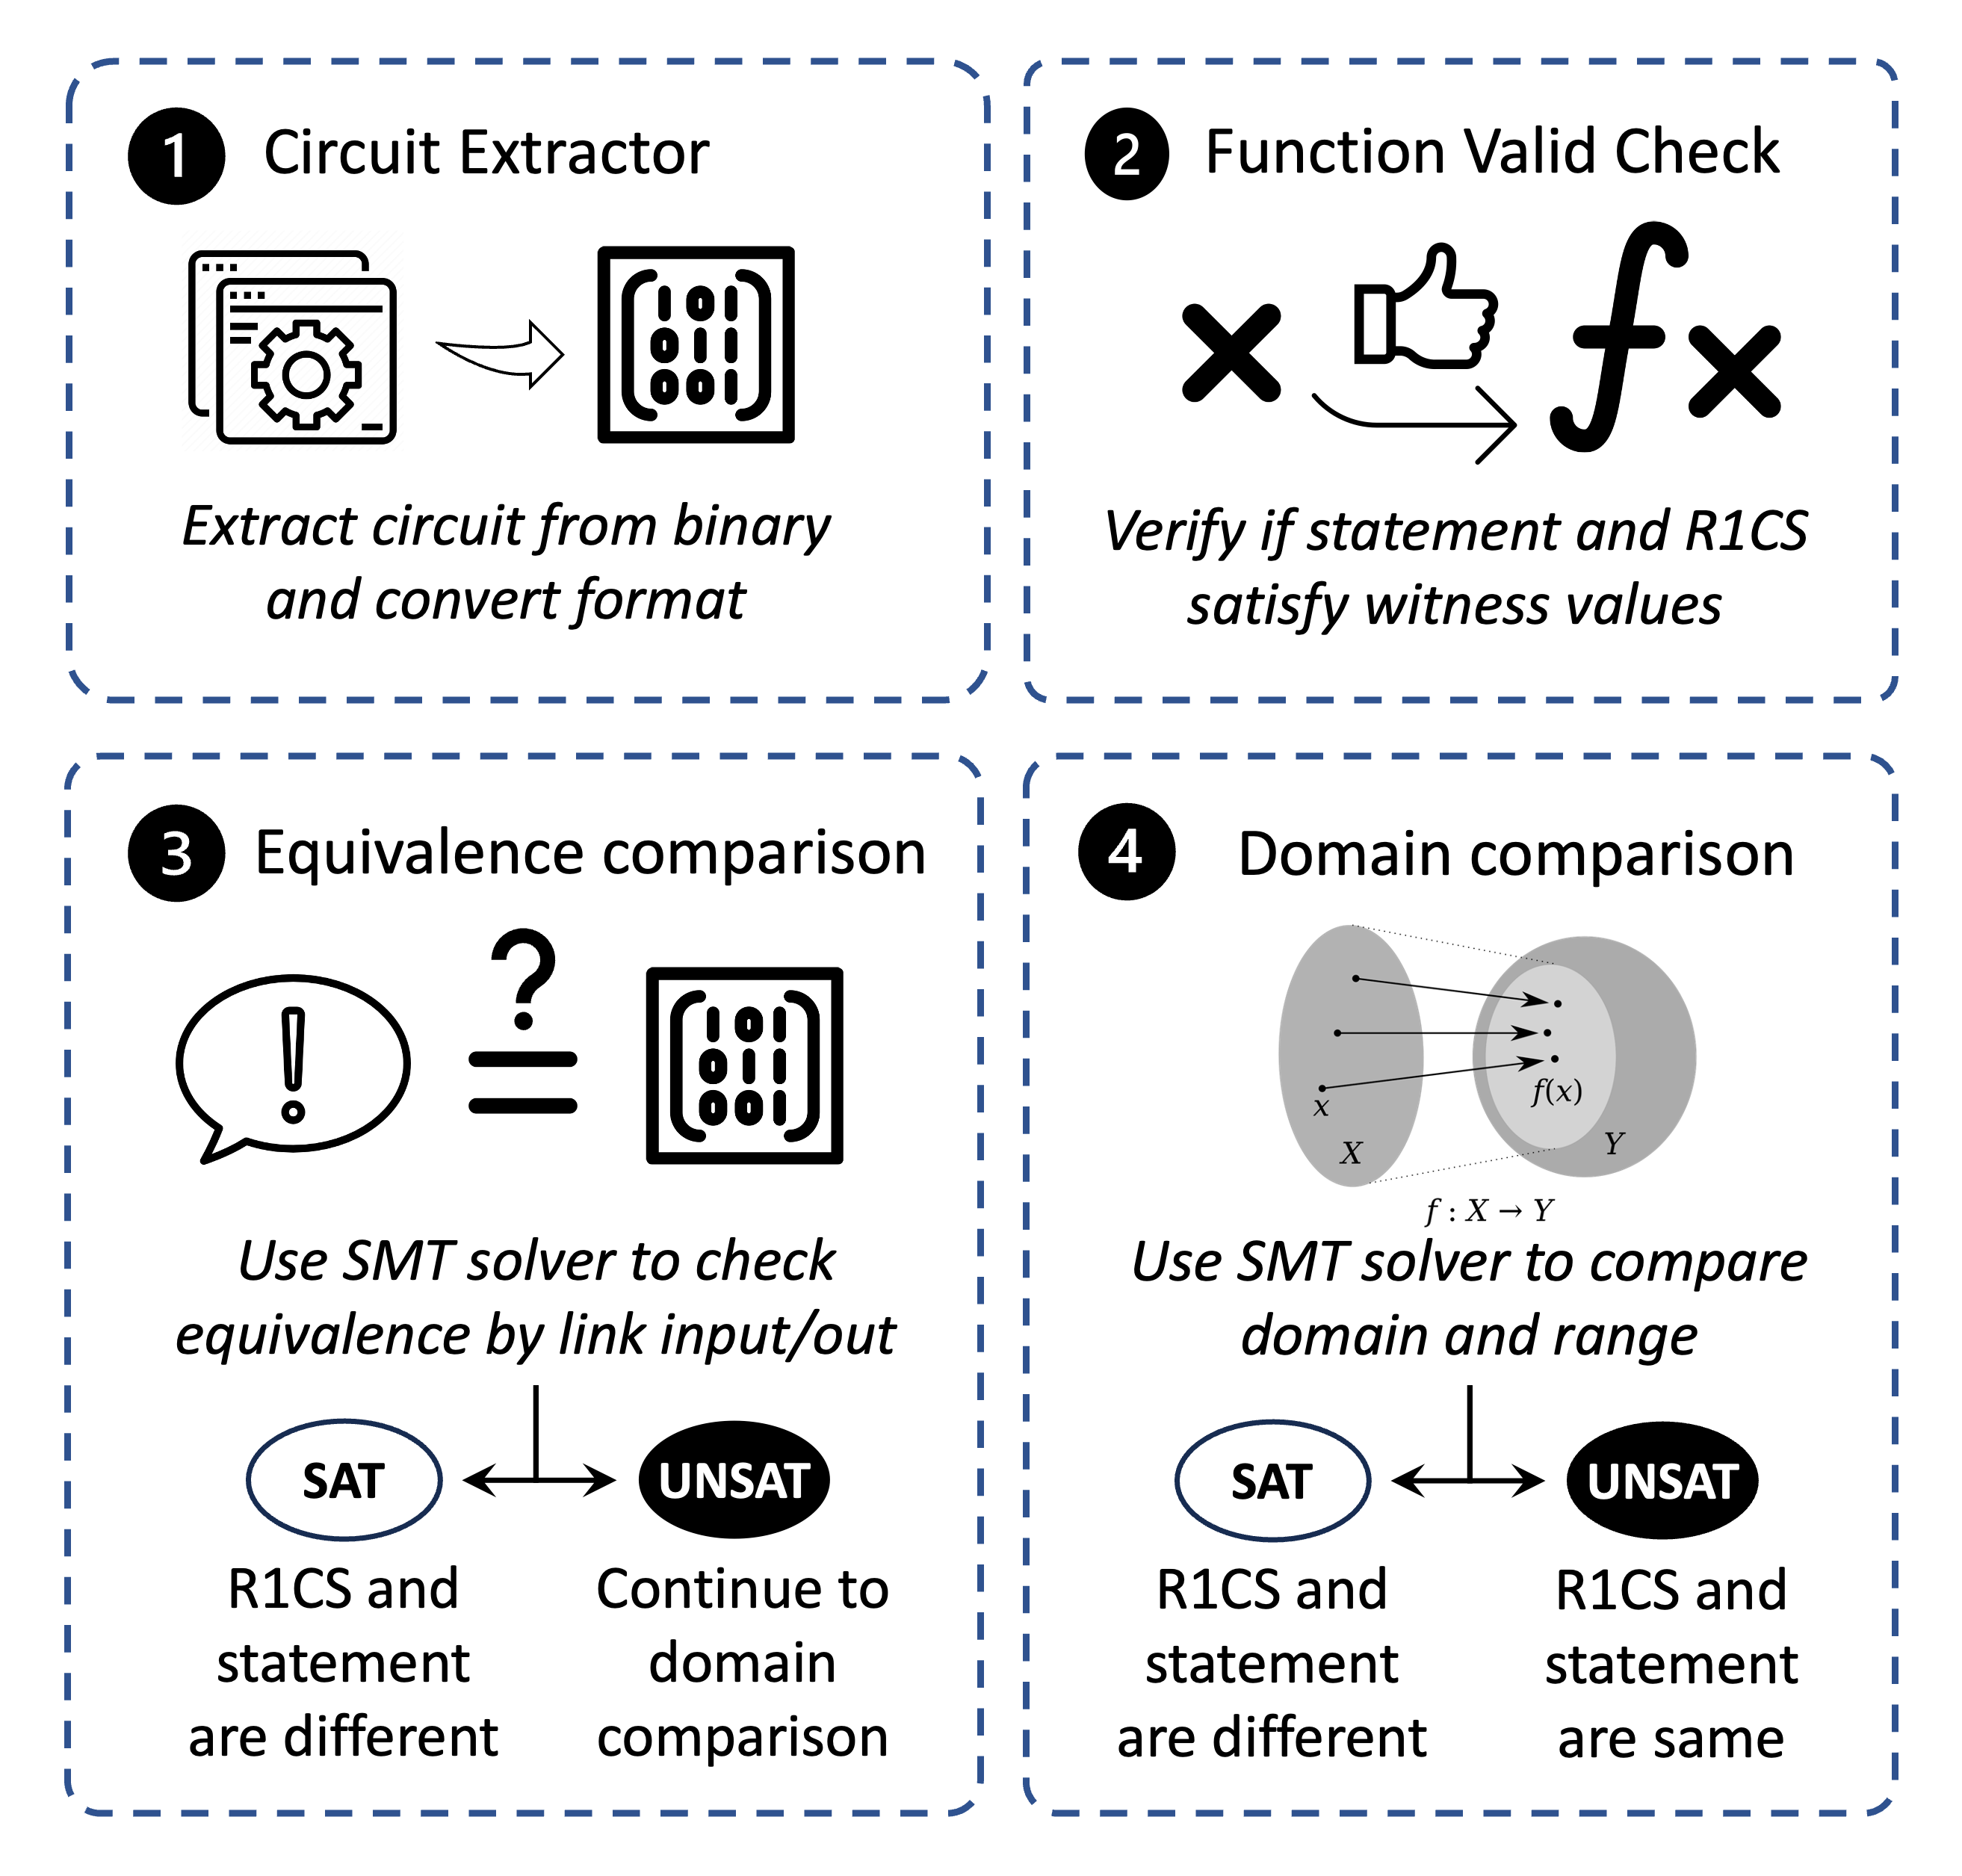
\includegraphics[height=2in]{ch-snarkprobe/figure/workflow_cc.png}
  \caption{\ConstraintChecker}
  \label{subfig:snarkprobe-workflow_cc}
\end{subfigure}
\hspace{-20pt}
\begin{subfigure}[b]{0.62\linewidth}
  \centering
  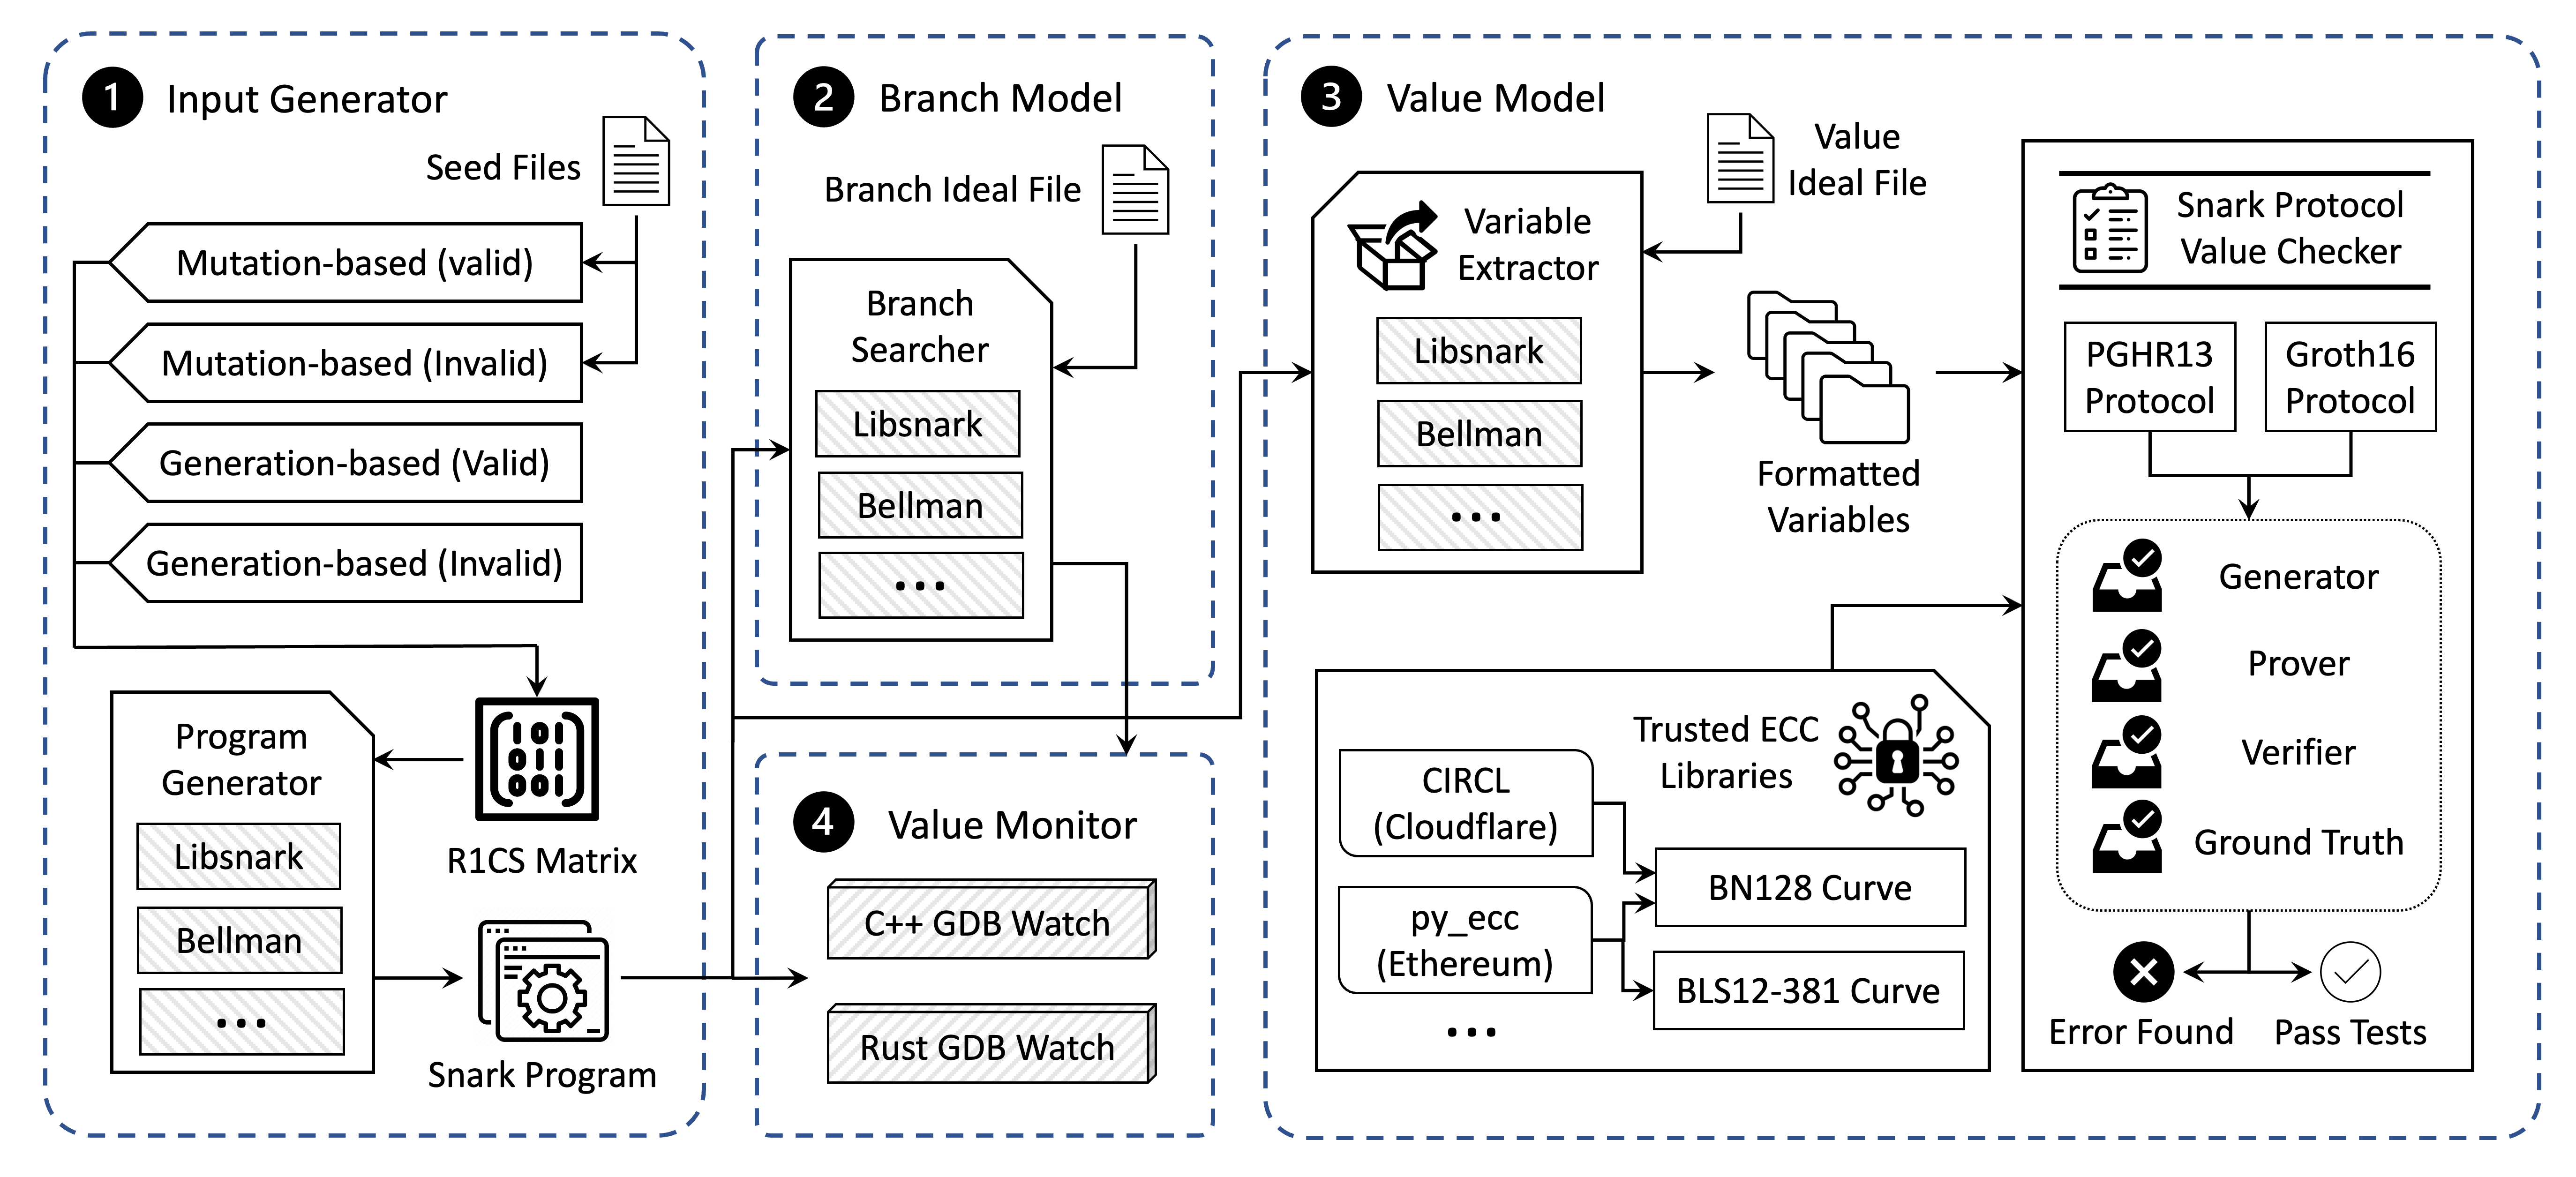
\includegraphics[height=2in]{ch-snarkprobe/figure/workflow_sf.png}
  \caption{\SnarkFuzzer}
  \label{subfig:snarkprobe-workflow_sf}
\end{subfigure}

\end{minipage}
\end{adjustbox}

\caption{Workflow of \tool. White boxes represent subcomponents universal for all zkSNARK libraries, forward diagonal stripes represent those designed for a specific library, and backward diagonal stripes represent those designed for a specific programming language.}
\label{fig:snarkprobe}
\end{figure}


\subsection{Workflow}

We now outline the workflow of running \tool, as well as establish terminology, before presenting the details and implementation in subsequent sections. \tool is composed of two broad sub-tools: the \ConstraintChecker and \SnarkFuzzer. These components can operate both independently of each other as well as in sequence, depending on what the user wishes to check.

Recall that at a high level, a \zksnark proof is generated in two main phases.  First (\textit{\circuitgen}), the user has a \textit{(proof) statement} that they wish to prove about, which requires converting this statement into a \textit{circuit} that the \zksnark protocol understands.
\textit{R1CS} is a specific form of this that we focus on in this work.  Second (\textit{\proofgen}), a \zksnark library takes the circuit (R1CS) as input and produces a proving key, verification key, and a \textit{proof}.


The first step verifies the consistency of a user-specified set of proof statement equations with the actual R1CS matrix used in the application, to ensure that the \circuitgen process generates the same proof as the developer states. The \ConstraintChecker uses an SMT solver to compare the input values, output values, domain, and range of the given statement equations with R1CS matrix to find any errors in the conversion. \autoref{subfig:snarkprobe-workflow_cc} shows the internal steps of the \ConstraintChecker, which we discuss in detail in \autoref{subsec:snarkprobe-constraintchecker}.


The second step checks the correctness of the library and \proofgen process. \autoref{subfig:snarkprobe-workflow_sf} shows the steps of \SnarkFuzzer, which we discuss in detail in \autoref{subsec:snarkprobe-snarkfuzzer}.
%%\fanyo{The \framework can evaluate the correctness of \zksnark library implementation.} 
First, the \inputgenerator produces an R1CS matrix (i.e., proof) using a variety of fuzzing techniques and compiles this into an executable proof program with the selected library, which serves as the input for the \branchmodel. Then, the \branchmodel investigates the visitation status for each branch during execution and provides feedback to the \inputgenerator to determine if another input is needed. This coverage feedback fuzzing helps improve the coverage rate of \SnarkFuzzer, which improves the chance of catching errors in the target library. Finally, the \valuemodel re-evaluates the protocol calculations to detect any potential cryptographic logic errors and looks for inconsistencies caused by unexpected value changes or implementation errors.
%%\fanyo{Since in the dynamic analysis, a single \framework evaluation cannot cover the entire library implementation. The \SnarkFuzzer will generates extra input seeds to execute multiple \framework check until the entire library has been fully evaluated.}

Together, these two components allow \tool to evaluate the end-to-end correctness and security of a specific implementation of a given proof statement for a given library (or to individually check different parts if desired).

Unlike standard fuzzers, \SnarkFuzzer can detect both software and \logicerror{s}.  We consider a \emph{software error} to be a bug or fault in the software that causes unintended behaviors or incorrect performance, such as crashing, overflow, or a system error.  A \emph{\logicerror}, on the other hand, is one that causes a program to produce an incorrect result due to errors in the cryptographic protocol implementation, such as incorrect mathematical operations or disregarding the specification. A \logicerror will not cause a software crash or raise an error message, making them much harder to detect.
For a basic example, in RSA, software errors might cause a program crash, but cryptographic logic errors are issues where the ciphertext value was not computed correctly ($m^e \mod N$ computed incorrectly) or too large a ciphertext was used (e.g., larger than the modulus).

%In general, \tool should be as automatic as possible, requiring little intervention from the developer.  However, there are still a few small manual pre-processing steps.
%First, to run the \ConstraintChecker, a user needs to indicate the proof statement.  After that, the \ConstraintChecker can run automatically to check the equivalence of the proof statement and circuit (R1CS).
%Second, before running \SnarkFuzzer, the user needs to manually create one ideal file containing the basic programming structure of the target library. However, this only needs to be done once ever per library that one wishes to test and could be done by anyone.
%We do not believe that these manual interventions require substantial cryptographic or zero-knowledge proof related expertise.

While we currently focus on R1CS-based zkSNARKS, we believe this high level design can be adapted without major changes to support additional (newer) types of proofs, particularly in the case of \SnarkFuzzer, which would largely only involve changing the input generation methodology and format.

\parhead{Why dynamic analysis?}
Dynamic analysis supports our goal of finding \logicerror{s} by allowing us to trace and extract real-time data and variable values, which we can then use to check for cryptographic protocol conformance and implementation errors.
It also allows us to easily support a number of different zkSNARK libraries written in different languages without the need for additional manual intervention, extensions, or program instrumentation by the user, making \tool flexible as well.
Our design choices mean that is easy to extend \tool to support new languages and libraries, without needing to investigate new instrumentation techniques or tools.

%In next two sections, we will go into more details and present how our tools detect errors in zk-SNARKs library. Section \ref{sec:design} introduces the design of the \ConstraintChecker and \SnarkFuzzer, and Section \ref{sec:implementation} demonstrates how we achieve our designs and the specific techniques we apply.

%\begin{figure*}[t]
  %\centering
  %\includegraphics[width=0.75\linewidth]{imgs/model.jpg}
	%\vspace*{-12pt}
  %\caption{Workflow in \SnarkFuzzer. White boxes represent subcomponents universal for all zkSNARK libraries, forward diagonal stripes represent those designed for a specific library, and backward diagonal stripes represent those designed for a specific programming language.}
  %\label{fig:snarkprobe-snarkfuzzer}
  %\vspace*{-8pt}
%\end{figure*}

%\parhead{Assumptions and Limitations.}
%Currently, \tool is a whitebox testing tool, and we assume that users have access to the program and library source code.  We leave extending \tool to work in a blackbox manner for future work.
%Also, \tool only works with R1CS-based zkSNARKs in our current implementation.  While we leave this for future work, we believe our high level design can be adapted without major changes to support additional (newer) types of proofs, particularly in the case of \SnarkFuzzer, which would largely only involve changing the input generation methodology and format.
%Finally, there are still a few small areas that require user intervention which we see as largely unavoidable in our current design, though we have sought to reduce these as much as possible and make them require the smallest amount of burden on or expertise from the user as possible.
%This includes the user indicating a proof statement for the \ConstraintChecker and the one-time per library creation of an ideal file containing the basic programming structure of the target library.

%\clg{Include some sort of short limitations paragraph.  For example, we require source code, there is still some manual effort needed (though a large amount of it only needs to be done once), etc.  Addressing these would be good avenues for future work.}
%\clg{Oh, we need to point out that this only works for R1CS based SNARKs, future work would then be to figure out how to adapt this to other, newer, types of SNARKs.}
%
%Even we remove most of the human affects in \tool, there are still a few manual interventions needed by our tools. \ConstraintChecker requires user allocating the public and private variables in correct order, or otherwise, \ConstraintChecker will raise a false alarm even the statement equations have been correctly converted into R1CS matrix. Meanwhile, developers also need to create the ideal files for \SnarkFuzzer when they want to test a new zk-SNARKs library or protocol. Creating ideal files is simply without requiring the understanding of high level zk-SNARKs knowledge. However, there is still some risks that developers may incorrectly implement the ideal files, and \SnarkFuzzer may have poor performance with ideal files that contains bias errors.
%
%\tool is a whitebox testing tool, and developers should have access to the program and library source code. A blackbox binary zk-SNARKs program cannot be examined by \ConstraintChecker and \SnarkFuzzer since our design can only handle the program compiled in debug mode. Also, \tool only works with rank-1 constraint system (R1CS) based on our current implementation, but this can be expanded in the future to adopt other, newer, types of zero knowledge proof without major revision in the high level design.
\section{Design and Implementation}
\label{sec:snarkprobe-design}

In this section, we introduce both the high level goals and concrete implementation decisions, tools, and techniques that allow us to realize \tool.  We start with the \ConstraintChecker and then discuss the various components of \SnarkFuzzer.  These two sub-tools can be used either in conjunction with each other, or separately, depending on what the developer wishes to check.

\subsection{\ConstraintChecker}
\label{subsec:snarkprobe-constraintchecker}

\parhead{Goals:} \emph{The \ConstraintChecker helps ensure that the realized proof is equivalent to a specified statement.  This also allows the \ConstraintChecker to find errors in flattening and/or gadget use.  It achieves this by comparing the equivalence of a user-specified proof statement and the compiled R1CS gates to ensure that the proof generated by the library represents the developer's specified statement\footnote{We note that we cannot do anything about the garbage-in-garbage-out problem (for example, the case where a developer implements a proof that misses a necessary case, such as omitting checking if a value is greater than 0).  We can just help determine if the specified statement and realized proof are likely equivalent.}.}

\parhead{Design.}%
The first step in generating a \zksnark proof is converting the desired proof statement equations into R1CS.  These R1CS gates should have the same domain, range, and output value as input statement equations.
To check this, we developed our \ConstraintChecker, which leverages an SMT solver and associated techniques to verify the equivalence of R1CS gates to the specified proof statement functions\footnote{We work around the general undecidability of function equality by operating in the more constrained setting (over the finite fields) and adding special rules for primary variables and auxiliary variables.}. To run the tool, the user only needs to write a short script to define the statement function, primary inputs, and auxiliary inputs in their zkSNARK proof, and everything else then happens automatically. \autoref{subfig:snarkprobe-workflow_cc} shows the key steps in the \ConstraintChecker, and we also provide an example in Listing \autoref{list:constraintchecker} of our \ConstraintChecker to show how a developer can run the tool. More examples can be found in our code. We note that our SMT solver could be replaced by any other techniques that allow one to check for function equality and fit the desired goals.
\definecolor{dkgreen}{rgb}{0,0.6,0}
\definecolor{gray}{rgb}{0.5,0.5,0.5}
\definecolor{mauve}{rgb}{0.58,0,0.82}

\lstset{
  frame=tb,
  language=Python,
  aboveskip=3mm,
  belowskip=3mm,
  showstringspaces=false,
  columns=flexible,
  basicstyle={\small\ttfamily},
  numbers=none,
  numberstyle=\tiny\color{gray},
  keywordstyle=\color{blue},
  commentstyle=\color{dkgreen},
  stringstyle=\color{mauve},
  breaklines=true,
  breakatwhitespace=false,
  breakindent=0pt,
  breakautoindent=false,
  xleftmargin=0pt,
  xrightmargin=0pt,
  framexleftmargin=5pt,
  framexrightmargin=0pt,
  tabsize=3
}

\begin{ZZlisting}[H]
\centering
\begin{adjustbox}{max width=\textwidth}
\begin{CenteredBox}
\begin{minipage}{0.96\textwidth}
\begin{lstlisting}
x = z3.Int("x")
## Indicate the public variables and private variables
allocate = ["x"]
variables = [x]
## Indicate the statement of a proof
statement = [x < 60]
## Provide the snark program to automatically extract the R1CS matrix
## Developer can also manually provide the R1CS matrix
path = os.path.join(currentdir, "range")
## Call the functions in ConstraintChecker to evaluate the correctness
fcmp = FunctionComparison(path)
fcmp.allocate(allocate)
fcmp.set_input_sizes(0)
fcmp.addVariables(variables)
fcmp.addStatement(statement)
fcmp.addGadget(gadget1.comparison_gadget("max")) ## Optional
fcmp.addRange(x, z3.And(x < 60))
fcmp.runComparisonTests()
\end{lstlisting}
\end{minipage}
\end{CenteredBox}
\end{adjustbox}
\caption{An example of \ConstraintChecker}
\label{list:constraintchecker}
\end{ZZlisting}
\parhead{Implementation.} The \ConstraintChecker contains two major components: the Circuit Extractor and a three-step equivalence check. We discuss these components in detail below. \autoref{pro:constraintchecker} presents the detailed procedure for each component. We discuss optimizations in \autoref{app:snarkprobe-constraintopt}.


\begin{protocol}[!htbp]
\centering
\begingroup
\makeatletter
\let\oldscriptsize\scriptsize
\renewcommand{\scriptsize}{\oldscriptsize\setlength{\baselineskip}{11.5pt}}
\makeatother

\setlength{\fboxsep}{6pt}
\setlength{\fboxrule}{0.35pt}

\vspace*{\fill}

\begin{adjustbox}{max width=\textwidth, max totalheight=0.92\textheight, keepaspectratio}
\begin{minipage}[t]{0.48\textwidth}

% ---------- (a) Parameters ----------
\fbox{%
\begin{minipage}[t]{0.95\textwidth}
\scriptsize
\raggedright
\setlength{\parindent}{0pt}
\setlength{\parskip}{0.35em}

\textbf{(a) Parameters.}

\begin{enumerate}[leftmargin=1.4em,itemsep=0.6em,topsep=0.25em,parsep=0.5em]
\item A set of statement equations $E_{1}$ in size $p$ where equation $e_{1}^{i} \in E_{1}$ and $i \in [1,p]$.
\item A set of equations $E_{2}$ converted from R1CS gates in size $q$ where $e_{2}^{i} \in E_{2}$ and $i \in [1,q]$.
\item $m$ private variables $x_{1}^{i}$ in $E_{1}$ where $i \in [1,m]$ and $n$ private variables $x_{2}^{i}$ in $E_{2}$ where $i \in [1,n]$ and $n \geq m$. A set of auxiliary input $v_{x}^{i}$.
\item $k$ public variables $y_{1}^{i}$ in $E_{1}$ and $k$ public variables $y_{2}^{i}$ in $E_{2}$ where $i \in [1,k]$. A set of primary input $v_{y}^{i}$.
\item A SMT Pro Solver $S$ and Optimizer $O$ with modulus $P$. $0 \leq x_{1} < P$, $0 \leq x_{2} < P$, $0 \leq y_{1} < P$, and $0 \leq y_{2} < P$ without optimization.

\vspace{0.5em}
\end{enumerate}
\end{minipage}%
}

\vspace{0.9em}

% ---------- SMT Solver ----------

\fbox{%
\begin{minipage}[t]{0.95\textwidth}
\scriptsize
\raggedright
\setlength{\parindent}{0pt}
\setlength{\parskip}{0.35em}

\textbf{SMT Solver:} The solver $S$ and optimizer $O$ are designed based on the Z3 theorem prover. Other SMT solvers may provide different solving interfaces.

\vspace{0.4em}

\textbf{Z3 Theorem Prover:} Z3 cannot directly model numbers as finite-field elements, so the modulus must be specified manually for each witness in the statement.

\vspace{0.5em}
\end{minipage}%
}

\vspace{0.9em}

% ---------- (b) Function valid check ----------
\fbox{%
\begin{minipage}[t]{0.95\textwidth}
\scriptsize
\raggedright
\setlength{\parindent}{0pt}
\setlength{\parskip}{0.35em}

\textbf{(b) Function valid check.}

INPUTS: $E_{1}$, $E_{2}$, $S$.

OUTPUTS: Boolean result of function validation.

\begin{enumerate}[leftmargin=1.4em,itemsep=0.6em,topsep=0.25em,parsep=0.5em]
\item Check and solve the R1CS gates:

Set a solvers $S_{1} \in S$.

Add $e_{1}^{i} \in E_{1}$ where $i \in [1,p]$ and range of $x_{1}^{i}$, $x_{2}^{i}$ to $S_{1}$.

Solve $S_{1}$ and get the set of private variables solution as $M^{i}_{1_{x}}$ and set of public variables solution as $M^{i}_{1_{y}}$.
\item Check and solve the statement equations:

Set a solvers $S_{2} \in S$.

Add $e_{2}^{i} \in E_{1}$ where $i \in [1,q]$ and range of $y_{1}^{i}$, $y_{2}^{i}$ to $S_{2}$.

Solve $S_{2}$ and get the set of private variables solution as $M^{i}_{2_{x}}$ and set of public variables solution as $M^{i}_{2_{y}}$.
\item Output $v_{x}^{i} \in M^{i}_{1_{x}}$ \textit{AND} $v_{x}^{i} \in M^{i}_{2_{x}}$ \textit{AND} $v_{y}^{i} \in M^{i}_{1_{y}}$ \textit{AND} $v_{y}^{i} \in M^{i}_{2_{y}}$.

\vspace{0.5em}
\end{enumerate}
\end{minipage}%
}
\end{minipage}
\hspace{0.7em}
\begin{minipage}[t]{0.48\textwidth}

% ---------- (c) Equivalent comparison ----------
\fbox{%
\begin{minipage}[t]{0.95\textwidth}
\scriptsize
\raggedright
\setlength{\parindent}{0pt}
\setlength{\parskip}{0.35em}

\textbf{(c) Equivalent comparison.}

INPUTS: $E_{1}$, $E_{2}$, $S$.

OUTPUTS: Boolean result of function equality.

Set two solvers $S_{1}$ and $S_{2} \in S$.

\begin{enumerate}[leftmargin=1.4em,itemsep=0.6em,topsep=0.25em,parsep=0.5em]
\item Comparing with public variables:

Add $e_{1}^{i} \in E_{1}$ where $i \in [1,p]$ and range of $x_{1}^{i}$, $y_{1}^{i}$ to $S_{1}$.

Add $e_{2}^{i} \in E_{2}$ where $i \in [1,q]$ and range of $x_{2}^{i}$, $y_{2}^{i}$ to $S_{1}$.

Add $x_{1}^{i} == x_{2}^{i}$ where $i \in [1,m]$ to $S_{1}$.

Add $y_{1}^{i} \neq y_{2}^{i}$ where $i \in [1,k]$ to $S_{1}$.

Check if $S_{1}$ is \textit{SAT}, \textit{UNSAT}, or \textit{UNSURE} as $c_1$.
\item Comparing with Boolean variables:

Set $b_1$ and $b_2 \in$ BOOLEAN.

Add $b_1 = \textit{AND}(E_{1})$ to $S_{2}$.

Add $b_2 = \textit{AND}(E_{2})$ to $S_{2}$.

Add $x_{1}^{i} == x_{2}^{i}$ where $i \in [1,m]$ to $S_{2}$.

Add $y_{1}^{i} == y_{2}^{i}$ where $i \in [1,k]$ to $S_{2}$.

Add $b_1 \neq b_2$ to $S_{2}$.

Check if $S_2$ is \textit{SAT}, \textit{UNSAT}, or \textit{UNSURE} as $c_2$.
\item Output ($c_1 ==$ \textit{UNSAT} \textit{AND} $c_2 ==$ \textit{UNSAT}).

\vspace{0.5em}
\end{enumerate}
\end{minipage}%
}

\vspace{0.75em}

% ---------- (d) Domain comparison ----------
\fbox{%
\begin{minipage}[t]{0.95\textwidth}
\scriptsize
\raggedright
\setlength{\parindent}{0pt}
\setlength{\parskip}{0.35em}

\textbf{(d) Domain comparison.}

INPUTS: $E_{1}$, $E_{2}$, $S$, $O$.

OUTPUTS: Boolean result of domain comparison.

\begin{enumerate}[leftmargin=1.4em,itemsep=0.6em,topsep=0.25em,parsep=0.5em]
\item Comparing upper and lower bond:

Add $e_{1}^{i} \in E_{1}$ where $i \in [1,p]$ and range of $x_{1}^{i}$, $x_{2}^{i}$ to $O$.

Add $e_{2}^{i} \in E_{1}$ where $i \in [1,q]$ and range of $y_{1}^{i}$, $y_{2}^{i}$ to $O$.

Solve the upper bond $u_{1}$ and lower bond $l_{1}$ from $O$.

Solve the upper bond $u_{2}$ and lower bond $l_{2}$ from $O$.
\item Check if R1CS is valid outside statement domain:

Add $\textit{NOT}(\textit{AND}(\text{range of }x_{1}^{i}, x_{2}^{i}))$ to $S$.

Add $e_{2}^{i} \in E_{1}$ where $i \in [1,q]$ and range of $x_{2}^{i}$, $y_{2}^{i}$ to $S$.

Check if $S$ is \textit{SAT}, \textit{UNSAT}, or \textit{UNSURE} as $c$.
\item Output ($c ==$ \textit{UNSAT} \textit{AND} $u_{1} == u_{2}$ \textit{AND} $l_{1} == l_{2}$).

\vspace{0.5em}
\end{enumerate}
\end{minipage}%
}
\end{minipage}
\end{adjustbox}

\vspace{0.5em}
\caption{Protocol of the \ConstraintChecker Using an SMT Solver}
\label{pro:constraintchecker}

\vspace*{\fill}

\endgroup
\end{protocol}


\parheadit{Circuit Extractor.} The Circuit Extractor can extract R1CS gates with private inputs, witness, and gadget relations from an executing zkSNARK binary program.  We do this using GDB.  We set a GDB breakpoint at the circuit declaration line, convert the circuit to an R1CS matrix when the program reaches the breakpoint, and save the formatted R1CS matrix for equivalence comparison. Automatic extraction both makes the tool more usable and reduces the potential for human errors in the equivalence comparison. Many zkSNARK libraries use Montgomery modular multiplication as an optimization. We also developed a Montgomery representation translator that can convert the Montgomery form to a standard integer format, so that our circuit extractor can produce a z3py (our SMT solver of choice) readable integer format.

After extracting the circuit, the \ConstraintChecker uses the SMT solver to verify the equivalence of functions through a three step process: a function valid check, equivalence comparison, and domain comparison. If one or more tests fail, then we determine that the given statement equation is not equivalent to the produced program. Otherwise, then we can provide assurances that it is highly likely that the proof realizes the specified statement correctly\footnote{We cannot \textit{guarantee} equivalence due to the fact that the SMT solver might output \texttt{UNKNOWN}, as well as possible domain gaps (see \autoref{app:snarkprobe-domaingap}).}.

\parheadit{Function Valid Check.} As the witness should be a solution in both the statement equations and equations built by the R1CS gates, we first create two SMT solvers $S_1$ and $S_2$ to verify that fact (see \autoref{pro:constraintchecker} (b)). The \ConstraintChecker considers the statement equations and R1CS gates to not be equivalent if the witness is not a valid solution for both.


\parheadit{Equivalence comparison.} The equivalence comparison verifies if the statement equations $y_1 = f(x_1)$ and R1CS gates $y_2 = f(x_2)$ have the same output for all the same inputs. First, the \ConstraintChecker creates a solver $S$, and adds $y_1 = f(x_1)$, $y_2 = f(x_2)$, $x1 = x2$ and $y_1 \ne y_2$ to the solver $S$ (see \autoref{pro:constraintchecker} (c)). If $S$ results in \texttt{SAT}, then the SMT solver has discovered that the statement equations and R1CS gates have a different output for at least one input and thus considers them not equivalent, and otherwise, it results in \texttt{UNSAT}. Like in many other use cases, the \ConstraintChecker cannot guarantee equivalency if the SMT solver returns \texttt{UNSAT} or \texttt{UNKNOWN}.
Note that the SMT solver may return \texttt{UNKNOWN} for a variety of reasons, including running out of memory, or if the quantifier-free fragment is undecidable (such as nonlinear integer arithmetic) or too ``expensive'' (such as finding primes $p*q = N$ for some $N$).
%Therefore, since the equations represented by an R1CS matrix are of the form $A * B - C = 0$, if the statement equation is not a quantifier-free formula, the SMT solver will never result in \texttt{UNKNOWN}.

\parheadit{Domain comparison.} The SMT solver cannot directly calculate an equation's domain, but it can find the maximum and minimum values for an equation (\autoref{subfig:snarkprobe-domaina} in \autoref{app:snarkprobe-domaingap} shows an example of different upper and/or lower bounds). We also use the SMT solver to find out if there is a gap between the domains' of the statement equations and R1CS gates, though we cannot guarantee to find all such gaps that may exist (see \autoref{app:snarkprobe-domaingap} for a detailed discussion).


%%%%%%%%%%

%\subsection{Design: \ConstraintChecker}
%\label{subsec:snarkprobe-constraintchecker}
%
%\parhead{Goals:} \emph{The \ConstraintChecker helps ensure that the realized proof is equivalent to a specified statement.  This also allows the \ConstraintChecker to find errors in flattening and/or gadget use.  It achieves this by comparing the equivalence of a user-specified proof statement and the compiled R1CS gates to ensure that the proof generated by the library represents the developer's specified statement\footnote{We note that we cannot do anything about the garbage-in-garbage-out problem (for example, the case where a developer implements a proof that misses a necessary case, such as omitting checking if a value is greater than 0).  We can just help determine if the specified statement and realized proof are likely equivalent.}.}
%
%Most common zkSNARK libraries do not require developers to understand the underlying zkSNARK protocol. However, in many instances, developers do have to convert the desired proof statement equations into R1CS, through a process which is generally called flattening. Many libraries will also use this format internally at some point as well.  These R1CS gates should have the same domain, range, and output value as input statement equations.
%
%In general, function equality is an undecidable problem since it is a form of the halting problem. However, we can work around this limitation as we only need to verify functional equivalence in a more constrained setting (over the finite fields). By adding special rules for primary variables and auxiliary variables, we can thus use SMT solvers to check for function equality.
%
%To do this, we developed a tool which we call the \ConstraintChecker that leverages an SMT solver and associated techniques to verify the equivalence of R1CS gates to the specified proof statement functions. To run the tool, the user only needs to write a short script to define the statement function, primary inputs, and auxiliary inputs in their zkSNARK proof. We note that our SMT solver could be replaced by any other techniques that allow one to check for function equality and fit the desired goals.
%
%
%% Figure \ref{fig:smt} shows the key steps in the \ConstraintChecker, which contains two major components: the Circuit Extractor and Equivalence Comparison. The Circuit Extractor extracts the necessary variables' values from the source program (including the R1CS if need be), while the Equivalence Comparison portion uses the SMT solver to verify the equivalence of functions through a three step process: a function valid check, equivalence comparison, and domain comparison. If statement equations and R1CS gates fail one or more tests, then we determine that the given statement equation is not equivalent to the R1CS gates in the program.  If all checks pass, then we can provide assurances that it is highly likely that the proof realizes the specified statement correctly\footnote{We cannot \textit{guarantee} equivalence due to the facts that the SMT solver might output an \texttt{UNSURE} result and possible domain gaps (see Section \ref{subsubsec:domain}).}.
%% Since the \ConstraintChecker compares R1CS directly to the user-specified proof statement, we can both check equivalence of R1CS that has been manually flattened by a developer, as well as R1CS that has been generated and compiled by a library.
%% We now discuss each of these subcomponents in more detail.
%
%% \parhead{Circuit Extractor} The Circuit Extractor can extract the R1CS gates with primary inputs, auxiliary inputs, and gadget relation from zkSNARK program file in binary. Extractor will save the circuit as R1CS matrix form, and \ConstraintChecker works for various zkSNARK libraries in different programming languages. Automatic extracting reduces the human intervention factor to avoid potential human errors in equivalent comparison.
%
%% \parhead{Function Valid Check}
%% The witness is the assignment of all variables, so witness should be a solution in both the statement equations and equations built by R1CS gates. Therefore, if witness is not a valid solution in R1CS gates equations, then, we consider the statement equation is not equivalent to R1CS gates. \yuquan{What about the case when witness is not a valid solution, but statement equation and R1CS gates are actually equal? Maybe we should say "we omit the case of invalid statement equations or invalid R1CS as they do not form a valid proof"?}
%
%% To verify if the statement equations and R1CS matrix is valid, we first create two SMT solvers $S_1$ and $S_2$. Next, add statement equations to $S_1$ and equations represented by R1CS matrix to $S_2$ (see Section \ref{algorithm} (b)). Finally, if witness is a solution of $S_1$ and $S_2$, then, we consider that the statement equations and R1CS gates are valid for the witness. Otherwise, \ConstraintChecker considers the statement equations and R1CS gates are not equivalence and there is no need to run equivalence and domain comparison test anymore.
%
%% \parhead{Equivalent comparison}
%% \label{subsubsec:snarkprobe-equivalentcomparison}
%% Equivalent comparison verifies if the statement equations $y_1 = f(x_1)$ and R1CS gates $y_2 = f(x_2)$ have the same output for all same inputs. Firstly, \ConstraintChecker creates a solver $S$, and add $y_1 = f(x_1)$, $y_2 = f(x_2)$, $x1 = x2$ and $y_1 \ne y_2$ to the solver $S$ (see Section \ref{algorithm} (c)). If $S$ results in \texttt{SAT}, then SMT solver discovers that the statement equations and R1CS gates have different output for at least one same input and consider statement equations and R1CS gates are not equivalent.
%% \new{Beside \texttt{SAT} and \texttt{UNSAT}, SMT solver may also return \texttt{UNSURE} when the solver does not have enough relations to determine the satisfiability of given equations. In this case, \ConstraintChecker cannot guarantee the equivalency between statement equations and R1CS matrix.} \yuquan{If it's \texttt{UNSURE}, do we treat it like \texttt{UNSAT}? Or how do we proceed with this result? I also wonder what is the odd of gettng \texttt{UNSURE}?}
%
%% \subsubsection*{Domain comparison}
%% \label{subsubsec:snarkprobe-domain}
%% SMT solver cannot directly calculate an equation's domain, but it can find the maximum and minimum value for an equation. Therefore, \ConstraintChecker uses the following steps to compare two equations' domains:
%
%% \textbf{Upper/Lower Bound:} \ConstraintChecker uses Optimizer in SMT solver to respectively find the upper bound and lower bound for statement equations and R1CS gates. If the lower bounds and upper bounds do not match, then, statement equations and R1CS gates do not have the same domain. Figure \ref{subfig:domaina} shows an example of statement equations and R1CS gates with different upper and/or lower bounds; Figure \ref{subfig:domainb} shows an example of statement equations and R1CS gates with the same upper and/or lower bounds.
%
%% \textbf{Domain Gap in R1CS Gates:} Same upper bound and lower bound does not guarantee that statement equations and R1CS gates have the same range. Figure \ref{subfig:domainc} shows an example of an unmatched domain with same upper bound and lower bound. Since the ground truth domain of statement equations is known and provided by developers, \ConstraintChecker uses SMT solver to find that if the statement equations have solution(s) outside the R1CS gates' \yuquan{Need confirm} domain. If SMT solver returns \texttt{SAT}, then the domains of statement equations and R1CS gates do not match and statement equations is not equivalent to R1CS gates.
%
%% \textbf{Domain Gap in Statement Equations:} Since the domain of R1CS gates is unknown, then \ConstraintChecker cannot use SMT solver to detect the unmatched domain as shown in Figure \ref{subfig:domaind}. However, this problem will not result generating a fake proof from zkSNARK library, but developers may not generate a proof with witness in the domain gap even their statement is valid. This type of gap is very rare, but we still try to find this issue by producing a set of uniform random numbers as input for statement equations and R1CS gates. If R1CS gates does not have a solution but statement equations has valid solution for an input number, then there is a gap in statement equations, which is not equivalent to the statement equations' domain. This test does not guarantee finding the domain gap, but a larger set of numbers has higher confidence in finding the gap. \blue{(probably need better way to explain this paragraph)} \yuquan{Why this case will not result in a fake proof? If an adversary finds this domain gap and input the witness within this gap into the statement equations, the corresponding R1CS turns out valid. Isn't it a successful attack?}
%
%
%
%
%\subsection{Impl: \ConstraintChecker}
%\label{subsec:snarkprobe-constraintcheckerimpl}
%
%Figure \ref{fig:smt} shows the key steps in the \ConstraintChecker, which contains two major components: the Circuit Extractor and Equivalence Comparison to check the equality between the desired proof statement equations and the actual R1CS matrix.
%Recall that we rely on the user only to write a very short specification defining the expected statement function, primary inputs, and
%auxiliary inputs in their zkSNARK proof.  Everything else then happens automatically.
%% Our Equivalence Comparison creates several solvers and optimizers in z3py as shown in Appendix~\ref{eqalgorithm}. At a high level, z3py solves the satisfiability of equations given a set of constraints and returns \texttt{SAT}, \texttt{UNSAT}, or \texttt{UNSURE}. z3py also has an optimizer that supports finding minimizing and maximizing values.
%
%%\begin{figure}[t]
  %%\centering
  %%%\captionsetup{justification=centering}
  %%\includegraphics[width=1.0\linewidth]{imgs/smt.jpg}
	%%\vspace*{-16pt}
  %%\caption{Procedure of Comparing the Equivalence of R1CS Gates and Statement Equations.}
  %%\label{fig:snarkprobe-smt}
  %%\vspace*{-8pt}
%%\end{figure}
%
%\subsubsection*{Circuit Extractor}
%The Circuit Extractor can extract R1CS gates with private inputs, witness, and gadget relations from an executing zkSNARK binary program.  It will save the circuit as an R1CS matrix form, allowing the \ConstraintChecker to work in a programming language agnostic manner. Automatic extraction both makes the tool more usable and reduces the potential for human errors in the equivalence comparison. Alternatively, users could also provide constraint and R1CS information manually (in the format our tool expects), without using the Circuit Extractor.
%
%We use GDB to do this extraction. In both the \pinocchio protocol and \groth16 protocol, the key generation function takes a circuit as input to compute the proving and verification keys. Therefore, our circuit extractor automatically sets a GDB breakpoint at the circuit declaration line, converts the circuit to an R1CS matrix when the program reaches the breakpoint, and saves the formatted R1CS matrix for equivalence comparison.
%
%Many zkSNARK libraries use Montgomery modular multiplication as an optimization. We also developed a Montgomery representation translator that can convert the Montgomery form of \libsnark and \bellman to a standard integer format, so that our circuit extractor can produce a z3py readable integer format.
%
%\subsubsection*{Equivalence Comparison}
%
%The Equivalence Comparison subcomponent uses the SMT solver to verify the equivalence of functions through a three step process: a function valid check, equivalence comparison, and domain comparison. If the statement equations and R1CS gates fail one or more tests, then we determine that the given statement equation is not equivalent to the produced program.  Otherwise, then we can provide assurances that it is highly likely that the proof realizes the specified statement correctly\footnote{We cannot \textit{guarantee} equivalence due to the fact that the SMT solver might output \texttt{UNKNOWN}, as well as possible domain gaps (see Appendix \ref{sec:domaingap}).}.
%
%\parhead{Function Valid Check:} As the witness should be a solution in both the statement equations and equations built by the R1CS gates, we first create two SMT solvers $S_1$ and $S_2$ to verify that (see Appendix \ref{eqalgorithm} (b)). The \ConstraintChecker considers the statement equations and R1CS gates to not be equivalent if the witness is not a valid solution for both.
%
%\parhead{Equivalence comparison:} The equivalence comparison verifies if the statement equations $y_1 = f(x_1)$ and R1CS gates $y_2 = f(x_2)$ have the same output for all the same inputs. First, the \ConstraintChecker creates a solver $S$, and adds $y_1 = f(x_1)$, $y_2 = f(x_2)$, $x1 = x2$ and $y_1 \ne y_2$ to the solver $S$ (see Appendix \ref{eqalgorithm} (c)). If $S$ results in \texttt{SAT}, then the SMT solver has discovered that the statement equations and R1CS gates have a different output for at least one input and thus considers them not equivalent, and otherwise, it results in \texttt{UNSAT}. Like in many other use cases, the \ConstraintChecker cannot guarantee equivalency if the SMT solver returns \texttt{UNSAT} or \texttt{UNKNOWN}.
%Note that the SMT solver may return \texttt{UNKNOWN} for a variety of reasons, including running out of memory, or if the quantifier-free fragment is undecidable (such as nonlinear integer arithmetic) or too ``expensive'' (such as finding primes $p*q = N$ for some $N$).
%%Therefore, since the equations represented by an R1CS matrix are of the form $A * B - C = 0$, if the statement equation is not a quantifier-free formula, the SMT solver will never result in \texttt{UNKNOWN}.
%
%\parhead{Domain comparison:} The SMT solver cannot directly calculate an equation's domain, but it can find the maximum and minimum values for an equation (Figure \ref{subfig:domaina} in Appendix \ref{sec:domaingap} shows an example of different upper and/or lower bounds). We also use the SMT solver to find out if there is a gap between the domains' of the statement equations and R1CS gates, though we cannot guarantee to find all such gaps that may exist (see Appendix \ref{sec:domaingap} for a detailed discussion).
%
%\parhead{An optimization for the SMT solver:} The SMT solver may take a while to solve some complicated equations. To reduce the processing time in the equality check, we introduce optimizations and simplify some equations in the R1CS matrix. For example, many \libsnark gadgets use bit shifting, which produces the equation $(x * (1 + (p - 1) * x)) \bmod p = 0$ in R1CS gates. This equation represents $x = 0$ or $x = 1$. For our optimization, if the \ConstraintChecker detects such a relation, it will be replaced with $0 \le x \land x \le 1$ where $x \in \mathbb{F}$. These are logically equivalent, but our replacement is much easier for the SMT solver to work with.  A real world gadget like the \texttt{comparison\_gadget} in \libsnark has 16 constraints, and there are 11 constraints representing $x = 0$ or $x = 1$ (see Appendix \ref{comparison}). %Therefore, this replacement optimization can significantly reduce the actual time to compare the equivalence between statement equations and R1CS gates.

%%%%%%%%%%



\subsection{\SnarkFuzzer}
\label{subsec:snarkprobe-snarkfuzzer}

\parhead{Goals:} 
\emph{\SnarkFuzzer is a smart fuzzing tool with the primary goal of finding potential logic or software errors in zkSNARK libraries. It produces zkSNARK programs with different proofs as input, to detect and catch these errors and provide full (important) code coverage.}

%\fanyo{We propose a dynamic white-box framework, \SnarkFuzzer, which can automatically verify if a \zksnark library implementation follow the \zksnark protocol and its security designs to potential logic or software errors. Since a single program may not call and use all branches in the library source code, we also involved fuzzing tool to generate multiple input seeds in order to verify the security of entire library.}

\SnarkFuzzer is composed of four major subcomponents: the \inputgenerator, \branchmodel, \valuemodel, and \valuemonitor. The \inputgenerator is responsible for generating an R1CS matrix and converting it to a zkSNARK program as input for the target library.  The \valuemodel and \valuemonitor are designed to detect implementation and cryptography related errors. The \branchmodel helps manage branch coverage and provides feedback to help \SnarkFuzzer decide if it needs to generate another input program. \autoref{subfig:snarkprobe-workflow_sf} shows the structure of \SnarkFuzzer with both its high level design as well as its implementation details.

\subsubsection*{\underline{\SnarkFuzzer: \inputgenerator}}
\label{subsec:snarkprobe-input-generator}

\textbf{Goals: } \emph{The \inputgenerator produces valid or invalid R1CS matrices and compiles them into executable proof programs for use by other components as testing inputs.  This should be done in a ``smart'' manner to help better catch errors.}

\parhead{Design.}%
The first step for our fuzzer is the generation of inputs to test a target library.  In \SnarkFuzzer, these inputs are simply valid or invalid R1CS matrices that represent a variety of (possibly random) proof statements.  To improve the chances of catching potential logic or software errors in the library, we desire this input generator to be ``smart'', in the sense that it should not just randomly generate inputs, but should take into consideration both the concept of valid/invalid proofs, as well as proof or R1CS edge cases.
At a high level, the \inputgenerator generates an R1CS matrix, and then the Program Generator uses this matrix to produce and compile an executable zkSNARK program with a given library. The compiled program will then be used as input for other components, like the \branchmodel, \valuemodel, and \valuemonitor.  Before generating the R1CS matrix, the \inputgenerator needs to decide on the size of the generated matrix (number of rows $n_r$ and columns $n_c$) and the number of public inputs $n_p$.  This can be done by simply choosing randomly, or in a smarter way by choosing from a specified distribution.
The \inputgenerator can be instantiated with any type of fuzzer that meets the aforementioned goals, giving it the flexibility and adaptability to use new techniques and tools, as they are developed.

%\subsubsection*{Matrix Size and Number of Public Variables}
%Before generating the R1CS matrix, fuzzer needs to decide the size of matrix (number of rows $n_r$ and number of columns $n_c$) and number of public input $n_p$. Table \ref{tab:range} shows the valid range for each variable. The standard random number generator can uniformly generate number in the valid range, but some sub-ranges are valueless than others, which means it is harder to trigger logic errors. Therefore, we use some probability distributions to generate these variables instead of the linear random number generator. The probability distributions can be easily replaced by another distribution if it produces R1CS matrix with a higher chance of catching the library errors. Table \ref{tab:range} shows the domain of valid matrix size and number of public variables.

%\begin{table}[h]
%\centering
%\hspace*{-0.1in}
%\begin{minipage}{\textwidth}
%{\small
%\begin{tabular}{l|l|l}
%Variable                   & Range                     & Valuable Sub-range  \\ \hline\hline
%Number of Row $n_r$          & $1 \le n_r$             & \multirow{2}{*}{$n_r$ different with $n_c$} \\ \cline{1-2}
%Number of Column $n_c$       & $2 \le n_c$             & \\ \hline
%Number of Public Input $n_p$ & $0 \le n_p < n_c$ & Near $0$ or $n_c -1$\\
%\end{tabular}
%}
%\end{minipage}
%\caption{The Range of Variables in the \inputgenerator \clg{Same comment that I put in Table 2, do we need this or is the text sufficient?}}
%\label{tab:snarkprobe-range}
%\end{table}

%\subsubsection*{Generation-based and Mutation-based Fuzzer}
%\inputgenerator in \SnarkFuzzer is a generation-based and mutation-based fuzzer that can produce zkSNARK program with ground truth by using the R1CS matrix representing invalid and valid proof as input.\yuquan{\inputgenerator in \SnarkFuzzer is a generation-based and mutation-based fuzzer, which produces zkSNARK programs using valid or invalid R1CS matrix as input.}
%
%Generation-based fuzzer produces a R1CS matrix from scratch, and these inputs provide unusual examples in real application as edge cases, providing better coverage to test the zkSNARK library. Generation-based fuzzer outputs a more diverse input set to test zkSNARK libraries than mutation-based fuzzer.
%
%However, it is hard to target some specific input types or library branches with generation-based fuzzer such as gadget format R1CS matrix. With mutation-based fuzzer, developers have full control to generate a specific type of R1CS matrix, and it will improve the efficiency of testing. At the same time, mutation-based fuzzer is quicker than generation-based fuzzer, so using large R1CS matrix as seed can reduce generating time when testing the library with R1CS matrix containing more constraints and variables. 

%\subsubsection*{zkSNARK Program Producer}
%After having R1CS matrix with number of public input, Program Producer can produce the source code for the proof statement represented by R1CS matrix with selected zkSNARK library such as \libsnark or \bellman. Then, Program Producer compiles the source code with library to an  executable binary program, which can be used as input for subsequent library testing.

\parhead{Implementation.}%
We developed four different methods of input generation to produce these matrices based on mutation-based and generation-based fuzzing.  These methods are complementary and all work in tandem to generate the fuzzing inputs (the user can specify the percentage of inputs generated by each method).  Each method targets a specific type of R1CS matrix to provide better overall coverage and comes with its own set of unique benefits (and trade-offs).

%The \inputgenerator is designed to produce zkSNARK programs by using both valid and invalid R1CS matrices as input.
%We developed four different methods of input generation to produce these matrices based on mutation-based and generation-based fuzzing.  These methods are complementary to each other and all work in tandem to help generate the fuzzing inputs (the user is able to specify the percentage of inputs generated by each method), allowing the \inputgenerator to be ``smarter'' than just random fuzzing.  We also use various probability distributions to generate random numbers for R1CS matrix size and the number of public variables.  Each of our four methods targets a specific type of R1CS matrix in order to provide better overall coverage and comes with its own set of unique benefits (and trade-offs), which we present now.

%\delete{Each of our four methods targets a specific type of R1CS matrix in order to provide better overall coverage. Invalid R1CS matrices produced by generation-based fuzzing can test a library with possible but unrealistic examples to explore some edge case errors that hard to reach by standard examples. Valid R1CS matrices produced by generation-based fuzzing simulates real world proof examples.  Additionally, the generation-based fuzzer does not depend on input seeds, so \SnarkFuzzer can still provide useful features even if a user cannot (or does not know how to) provide beneficial input seeds. In the other set of techniques, R1CS matrices produced by mutation-based fuzzing can work off of some input examples that are hard to produce by generation-based fuzzing. This subcomponent can also replace the generation-based fuzzer to produce some valid large R1CS matrices in a short time, thus reducing the overall runtime of \SnarkFuzzer, since generation-based fuzzing may require a lengthy amount of time to produce a large valid R1CS matrix.
%\clg{I'm not sure sub \inputgenerator is quite the right term here, but I'm not really sure what to call them.  We can brainstorm on this a little.}
%\yuquan{Maybe matrix generator or matrix randomizer? Also, do we also like another name for \inputgenerator? I personally feel its a bit misleading as well, maybe SNARK generator?}}

%\begin{figure}
%\centering
%\begin{subfigure}{0.2\textwidth}
  %\includegraphics[height=1.2in]{imgs/matrix-size.png}
  %\vspace{-0.5cm}
  %\caption{Sub-caption 1 \footnotemark \clg{we should label the axes in these figures -- also what do the 0.5 steps mean on the x-axis?}}
  %\label{subfig:snarkprobe-matrix_size}
%\end{subfigure}
%\hspace{1em}
%\begin{subfigure}{0.2\textwidth}
  %\includegraphics[height=1.2in]{imgs/num-pub-input.png}
  %\vspace{-0.5cm}
  %\caption{Variable $n_p$}
  %\label{subfig:snarkprobe-num_pub}
%\end{subfigure}
%\vspace{-0.2cm}
%\caption{Random Number Generator Distribution}
%\label{fig:snarkprobe-random}
%%%\vspace{-3mm}
%\end{figure}
%\footnotetext{Note, depending on the matrix size, the random number generator may produce more pairs towards the middle of the distribution as there are many more ways to obtain them (similar to what happens when you toss two dice and record the sum).}

%\parheadit{Matrix Size and Number of Public Variables.}
%To increase the chance of finding an error during fuzzing, the \inputgenerator can handle a variety of different distributions for random number generation. For example, as is often the case with traditional fuzzing, we assume that extremes are more likely to cause errors, and we thus guess that we will be more likely to trigger logic errors when the number of public variables is near $0$ or $n_c - 1$. Therefore, we can use an inverse normal distribution to generate the number of public variables.

% \parhead{Number of Variables and Constraints.} We consider that a non-square R1CS matrix has the higher chance of triggering a logic error, \clg{Why did we decide this again?  I can't remember what the logic was for why this was more likely to cause errors?  Was it not just because this might be something more realistic?} so the \inputgenerator generates fewer pairs of $n_r$ and $n_c$ such that $|n_r - n_c|$ is close to $0$. To follow this rule, we select the triangle distribution as shown in Figure \ref{subfig:matrix_size}, where the x-axis indicates the value of $|n_r - n_c|$, and y-axis indicates the count to get the pair. \clg{What do you mean the ``count to get the pair''?}  Therefore, our \inputgenerator will generate a roughly square R1CS matrix with lower probability.  This distribution is quite easy to change though, and can be tweaked to reflect the user's desired distribution.

% \parhead{Number of Public Variables.} As is often the case with traditional fuzzing, we assume that extremes are more likely to cause errors, and we thus guess that we will be more likely to trigger logic errors when the number of public variable is near $0$ or $n_c - 1$.  To model this, we use an inverse normal distribution to generate $n_p$ as shown in Figure \ref{subfig:num_pub}, where the x-axis indicates the value of the random number, and the y-axis indicates the count to get the value.\clg{Again, not sure what you mean by ``count'' here?} Therefore, the \inputgenerator will output more R1CS matrices with the number of public variables near $0$ and the specified total number of variables.

%\begin{table}[t]
%\centering
%\hspace*{-0in}
%\begin{minipage}{\textwidth}
%{\footnotesize
%\begin{tabular}{l||l|l}
%Fuzzer Type                      & Matrix Type    & Fuzzing Method                    \\ \hline\hline
%\multirow{2}{*}{Generation} & Invalid Matrix & Random witness w/ random matrix \\ \cline{2-3} 
                                  %& Valid Matrix   & Random witness w/ solved matrix \\ \hline
%\multirow{2}{*}{Mutation}   & Invalid Matrix & Mutate values in matrix           \\ \cline{2-3} 
                                  %& Valid Matrix   & Multiply matrix and witness       \\ 
%\end{tabular}
%}
%\end{minipage}
%\caption{Four Fuzzing Methods in the \inputgenerator \clg{Do we need this table?  Does it add anything given that we discuss all of this in the text?  It is definitely a nice concise summary of the techniques, but also, space :)}}
%\label{tab:snarkprobe-fuzzer}
%\end{table}

\parheadit{Generation-based invalid matrix.}
Our generation-based fuzzer is designed to create an R1CS matrix from scratch.  Generation-based fuzzing has the advantage of not depending on input seeds, allowing it to function without (user) input.
The random number generator will generate $n_r * n_c$ integers as an R1CS matrix and $n_r - 1$ integers as the witness $w$ (since the first value of the witness is always equal to 1), and we use the constraint relation $w \cdot A \times w \cdot B - w \cdot C = 0$ to verify the ground truth of the matrix. This tests a library with possible but unrealistic examples to search for edge case errors that are hard to reach with traditional examples.

%\delete{While we are trying to generate an invalid matrix in this instance, there is a very small chance that this randomly genereated matrix and witness are valid constraints.  The \inputgenerator will confirm that our generated values are indeed invalid by using the constraint relation $w \cdot A \times w \cdot B - w \cdot C = 0$. In all, the \inputgenerator needs to generate $n_r * (n_c + 1)$ integers to produce an invalid R1CS matrix.}

\parheadit{Generation-based valid matrix.}
To produce a valid matrix that simulates a real world proof example, the random number generator will generate $n_r - 1$ integers as a witness $w$. Then, a valid matrix will be calculated with z3py based on this witness and the constraints relations in $w \cdot A \times w \cdot B - w \cdot C = 0$. Depending on the actual values in the randomly chosen witness, the complexity of solving the equations to fill out the matrix may vary, but a larger matrix (i.e., larger witness) usually results in a longer generation time.  As such, we recommend that for testing large R1CS matrices, the generation-based fuzzer is run once to generate an input seed that can be given to the mutation-based fuzzer.

\parheadit{Mutation-based invalid matrix.}
The mutation-based fuzzer requires an R1CS matrix with a number of public variables as a seed, and then flips values to generate a new matrix. We use Atheris, a mutation-based, coverage-guided fuzzer developed by Google \cite{atheris}. The seed is converted into a byte array, then Atheris will flip the array, and then it is converted back to a (new) R1CS matrix.  Because we have randomly flipped values in the matrix, the R1CS constraint relations will be destroyed, and the matrix will be invalid.  This technique can work off of and mutate input examples that might be hard to produce by generation-based fuzzing.

\parheadit{Mutation-based valid matrix.}
Our mutation-based fuzzer can also produce a valid R1CS matrix. Instead of flipping random values, a random number $c$ will be generated, and the new matrix $M$ will be calculated based on the seed matrix $M_0$ as $M = c M_0$.
% where $M, M_0 \in \mathbb{F} ^ {m \times n}$ and $c \in \mathbb{Z}$.
This multiplication will not break the constraint relations, so the new matrix is still valid.  This can be used with the generation-based fuzzer to produce valid large R1CS matrices in a short time, thus increasing performance.

%\parheadit{Provided seeds for the mutation-based fuzzer.}
%We provide a few R1CS matrix seeds for the mutation-based fuzzer to cover some specific library branches and matrix structures. For example, \libsnark re-formats certain R1CS matrices for optimization purposes, and we provide such matrix as a seed to quickly hit the optimization function branch. We also provide large matrix seeds so one does not necessarily need to run the generation-based fuzzer.

%\delete{However, our generation-based fuzzer may never produce a matrix that fits this optimization, so we provide a seed matrix that can hit the optimization function in \libsnark and exercise that code path. Additionally, when a matrix is too large (such as larger than $1000 \times 1000$), z3py takes quite a long time to calculate a valid matrix. Therefore, to save generation time, we also provide as seeds, so the generation based fuzzer only needs to deal with smaller matrices.}


\subsubsection*{\underline{\SnarkFuzzer: Ideal Files}}
\label{subsec:snarkprobe-ideal-files}

\parhead{Goals:} \emph{The ideal files act as a guide for the \branchmodel and \valuemodel to check code coverage and protocol calculations. They contain information related to the source zkSNARK library such as branch locations, variable names, and data types.}

\parhead{Design.}%
Each library and protocol needs two ideal files: an ideal branch file that contains the locations of the branches in a library (automatically generated), and an ideal value file that contains information about the variables in a program (manually generated).  
Manually creating the ideal value file does not require any specialized knowledge related to zkSNARK protocols, the library, or cryptographic techniques, and the user only needs basic skills such as defining functions, conditions, and assigning variables.
These ideal files can be reused for any program using the same protocol and library.

\parheadit{Ideal Branch File.}%
An ideal branch file contains protocol-specific information related to the branches in a library.  Function calls, if-conditions, and loops are all considered branches.
The branch file also contains information about \texttt{IMPORTANT} versus \texttt{UNIMPORTANT} branches to help the \valuemodel.  Important branches include cryptographic calculations and other core protocol components that we wish to ensure testing and coverage of, while unimportant branches are those that do not involve relevant computation.
%\fanyo{Branch line number information can be listed automatically, but user still need to manually mark each branch as \texttt{IMPORTANT} or \texttt{UNIMPORTANT}. (Not sure if we should metion in there or next section)}

%\parhead{Important and Unimportant Function:} Fuzzer tries to cover as many branches, especially all crypto-related branches, such as functions with elliptic-curve cryptography calculation and math computation, in the library as possible by generating numerous inputs. We marked these types of branches as \texttt{IMPORTANT}, and fuzzer will continuously generate new input until cover all important branches.
%
%Meanwhile, \SnarkFuzzer does not need to spend extra time in generating new input program to cover the branches that do not involve in cryptography related calculation, and these branches should be marks as \texttt{UNIMPORTANT}, and \inputgenerator stops generating new inputs even \SnarkFuzzer does not cover all unimportant branches in the library. Labeling branch does not require any cryptographic related knowledge.

% \delete{However, there are many functions or conditions in the library that do not involve any zkSNARK protocol or general mathematics calculation, and they do not have side effects to any variables. These types of branches in the library are valueless, and \SnarkFuzzer does not need to spend extra time in generating new input program to cover these branches. Therefore, we marked these types of functions, conditions, and returns as \texttt{UNIMPORTANT}, so \inputgenerator can stop generating new inputs even \SnarkFuzzer does not cover all unimportant branches in the library.}

% \delete{Marking branches as \texttt{IMPORTANT} or \texttt{UNIMPORTANT} does not require zkSNARK protocol knowledge, since decision can be made without the understanding of functions. If developers do not have confidence to classify a branch as \texttt{UNIMPORTANT}, then this branch should be marked as \texttt{IMPORTANT} because marking a few \texttt{UNIMPORTANT} as \texttt{IMPORTANT} only slightly increase \SnarkFuzzer running time, but it ensures that \SnarkFuzzer will not miss any errors or bugs in the tested library.}

\parheadit{Ideal Value File.}%
An ideal value file contains location information for all variables that must be used to evaluate the protocol calculation. The \valuemodel will use line and path information in this file to extract all variables' values. Only variables defined in the official protocol paper should be added to the ideal value file.


\parhead{Implementation.}%
We have already developed the ideal files for \pinocchio and \groth16 in \libsnark and \groth16 in \bellman, \arkworks, and \gnark.

\parheadit{Ideal Branch File.}%
By default, all branches are marked as \texttt{IMPORTANT} and thus covered.  We asked four researchers in our group (including people with experience using zkSNARKs and those with only programming experience) to label branches as \texttt{IMPORTANT} or \texttt{UNIMPORTANT}. To ensure \SnarkFuzzer does not miss any critical components, only branches labeled as \texttt{UNIMPORTANT} by all four researchers could be marked as \texttt{UNIMPORTANT} in our example ideal branch files\footnote{Incorrectly labeling \texttt{UNIMPORTANT} branches as \texttt{IMPORTANT} only increases the fuzzing time without affecting the accuracy of the analysis.}. We provide an example snippet of an ideal model file for \libsnark in \autoref{fig:ideal_branch}.

\begin{figure}[H]
\begin{tcolorbox}
\begin{verbatim}
Relative Path: knowledge_commitment/kc_multiexp.tcc
FUNCTION,2,99,127,kc_batch_exp_internal,IMPORTANT
CONDITION,4,117,124,2,IMPORTANT
CONDITION,5,119,123,2,IMPORTANT
RETURN,2,126,126,2,IMPORTANT
\end{verbatim}
\end{tcolorbox}
\caption{Example file for the ideal branch file}
\label{fig:ideal_branch}
\end{figure}

%\textbf{Static Analysis for Call-graph:}
% As is the case with many libraries, some zkSNARK libraries, such as \libsnark, are large and contain many extra features. As such, the library may contain some uncallable/unreachable functions that have been marked as important. For example, \libsnark has two crypto-related functions \texttt{r1cs\_to\_qap\_instance\_map} and \texttt{r1cs\_to\_qap\_instance\_map\_with\_evaluation}. These two functions were marked as important based on the previous principles. However, \texttt{r1cs\_to\_qap\_instance\_map} is not called by any other functions in the code, including the main function, so it will not be used as part of any proof. Therefore, we should exclude these kinds of functions in the ideal branch file since they cannot be exercised.

In order to find uncallable functions, we used a static analysis tool called Doxygen \cite{doxygen} to draw the library functions' call graph. %Doxygen supports many popular languages and can generate documentation, including call graphs, from annotated library sources.
%\libsnark, for example, already includes a Doxygen configuration file in its source repository. 
Doxygen can help a user generate the call graph for a library, and by using this call graph, the user can easily find unused and uncallable functions to reduce fuzzing costs.

\parheadit{Ideal Value File.}%
The ideal value file contains ``official'' variable names, variable types, and variable names, path, and line number (the final assignment location for a variable) in the library's source code. We provide an example snippet of an ideal value file for the \libsnark library in \autoref{fig:ideal_value}.
While line numbers might change as code is maintained, one should not need to manually create a new file often.  If there are only minor or non-cryptographic related changes, our tool will automatically match the new line numbers.


\begin{figure}[H]
\begin{tcolorbox}
\begin{verbatim}
tau,Fr,t,zk_proof_systems/.../r1cs_ppzksnark.tcc,252
rhoA,Fr,rA,zk_proof_systems/.../r1cs_ppzksnark.tcc,300
rhoB,Fr,rB,zk_proof_systems/.../r1cs_ppzksnark.tcc,301
\end{verbatim}
\end{tcolorbox}
\caption{Example file for the ideal value file}
\label{fig:ideal_value}
\end{figure}


%%%%%%%%%%



\subsubsection*{\underline{\SnarkFuzzer: \branchmodel}}
\label{subsec:snarkprobe-branch-model}

\textbf{Goals: } \emph{The \branchmodel monitors and records branch visitation status as \SnarkFuzzer runs, and informs and stops it after all \texttt{IMPORTANT} branches have been covered.}

\parhead{Design.}%
The \branchmodel is used to evaluate if the target library has been fully tested. Traditional fuzzers often work by examining utilized memory bytes in a binary or lines of source code hit to check for program coverage, and then mapping this coverage to an input to determine the next one.  However, in a zkSNARK library, it is difficult to correlate the exact relation between a specific branch and values in the input program that could trigger it. Therefore, we instead use the idea of function and condition branches to evaluate coverage.

%\fanyo{It is impossible to achieve full code coverage with a single input program \framework evaluation if a library has at least one branch.}
Since any unvisited branches may cause errors, the \branchmodel evaluates each input program to acquire the list of branches that the program visited. The \inputgenerator will continuously generate new program inputs with different proof statements/matrices until all \texttt{IMPORTANT} branches have been visited.

To ensure that we achieve both breadth and depth in code coverage, the \branchmodel also works to ensure that each branch is covered multiple times with different inputs, keeping a count of the number of times each \texttt{IMPORTANT} branch is hit. We allow the user to define a visitation threshold to balance performance with coverage and confidence.
As more inputs are generated, we have a higher chance of finding potential issues in the target library or, conversely, more confidence that the target library is safe, at the cost of runtime.


\parhead{Implementation.}%
Our \branchmodel uses GDB breakpoints to investigate the visitation status for each branch defined in the ideal branch file. A GDB breakpoint stops the program whenever the selected location in the program is reached for debugging, and it can be set by line number, function name, or address in the program.  When the \inputgenerator produces a zkSNARK program, the \branchmodel sets a GDB breakpoint at the start line for each branch. If a branch is then visited during runtime, GDB will temporarily stop the input program at the corresponding breakpoint. After the program is finished running, the \branchmodel records a list of visited branches for the current program. If all important branches have not been visited at least once, or the visitation threshold has not been met, the \branchmodel will instruct the \inputgenerator to generate a new program with a different proof until all important branches have been covered.

%%%%%%%%%%



\subsubsection*{\underline{\SnarkFuzzer: \valuemodel}}
\label{subsec:snarkprobe-value-model}

\textbf{Goals: } \emph{The \valuemodel's goal is to find \logicerror{s}, such as inconsistencies with the protocol definition or incorrect cryptographic operations.}

\parhead{Design.}%
The \valuemodel is one of the most important components in \SnarkFuzzer, and one of the biggest improvements compared with other fuzzers. Its job is to detect cryptographic logic errors in a library.  At a high level, the \valuemodel must extract all necessary variable values from the input program, which it then feeds to the other components.
%It then feeds this information to other components that will work to detect implementation errors and protocol calculation errors, such as unexpected side effects, misinterpretation of the protocol, and/or miscalculations during optimization or simplification.
It achieves this through two major sub-components: the \valueextractor and \valuechecker.

\parheadit{\valueextractor.}
The \valueextractor extracts variables' values from the source zkSNARK program, which are then used in the \valuechecker.  The ideal value file provides a list of variables that need to be extracted. Then, the \valueextractor recursively extracts these values from the last assignment location in the program and library, and reformats the values to the \valuechecker readable format.

\parheadit{\valuechecker.}
The \valuechecker re-evaluates all protocol calculations and compares these ground-truth values to the values extracted from the input program by the \valueextractor to find any possible logic errors.
%Many zkSNARK libraries have optimizations to reduce their runtime, such as avoiding unnecessary repeated pairings or exponentiations, which bring a risk of being incorrectly implemented.
In the re-evaluation process, the \valuechecker will faithfully follow the protocol from the formal specification without any optimization, simplification, or reformatting.  To build a trustable re-evaluation process, our \valuechecker uses ECC libraries that have been tested and widely used.  In the future, this component could be replaced by any trusted evaluation source, such as a formally verified implementation.


\parhead{Implementation.}%

\parheadit{GDB PrettyPrint.}%
%\label{subsubsec:snarkprobe-prettyprint}%
GDB can display both the structure and value(s) for a variable. However, for more complicated variables 
GDB displays some unnecessary variable structure and data. Also, different libraries usually have different data structures (even for the ``same'' variables), and, as such, the \valuechecker cannot directly use the raw, unformatted variable value extracted from the library. For example, \autoref{subfig:snarkprobe-prettyprint_a}, \autoref{subfig:snarkprobe-prettyprint_b}, and \autoref{subfig:snarkprobe-prettyprint_c} show a $G_1$ type variable that represents the same number in both \libsnark, \bellman, and \arkworks but has different structure and value when printed naively.
%without PrettyPrint in both \libsnark and \bellman, and they represent the same number in finite field but with different structure and value (due to the different finite field and elliptic curve modulus).

To make the \valuechecker more universal, we developed a PrettyPrint functionality for each library to convert all data structures into the same format. The goals of PrettyPrint are twofold: $1)$ to allow the extractor to keep only the necessary values for a variable, and $2)$ to convert the same types of variables from different libraries into a common universal format that the \valuechecker can then accept. \autoref{subfig:snarkprobe-prettyprint_d} shows an example of the PrettyPrint result for the same $G_1$ variable as before. %Therefore, with PrettyPrint, the \valuechecker can be easily applied to any library, even in different programming languages, since PrettyPrint can consistently convert all data structures into the same, more straightforward format.


\begin{figure}[t]
\centering
\begin{subfigure}{0.9\textwidth}
  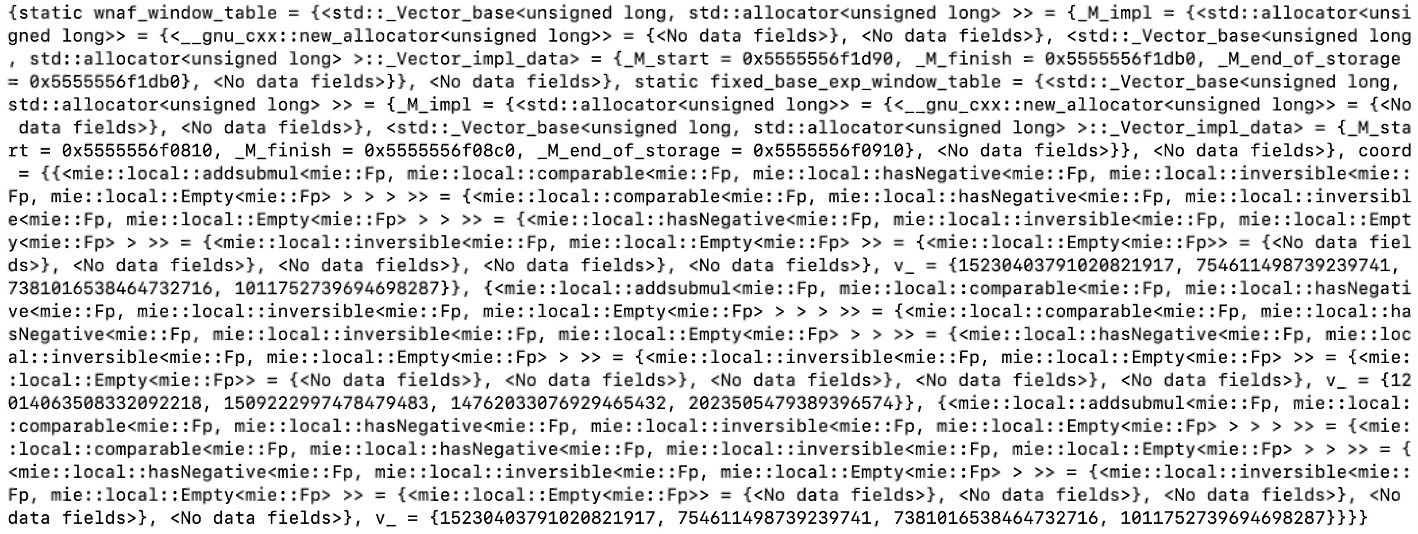
\includegraphics[width=\textwidth]{ch-snarkprobe/figure/prettyprint-a.jpg}
  \caption{Content without PrettyPrint in \libsnark}
  \label{subfig:snarkprobe-prettyprint_a}
\end{subfigure}
\par\vspace{10pt}
\begin{subfigure}{0.9\textwidth}
  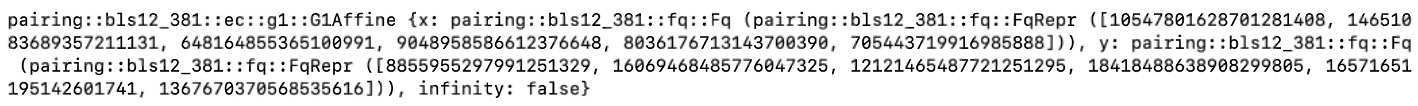
\includegraphics[width=\textwidth]{ch-snarkprobe/figure/prettyprint-b.jpg}
  \caption{Content without PrettyPrint in \bellman}
  \label{subfig:snarkprobe-prettyprint_b}
\end{subfigure}
\par\vspace{10pt}
\begin{subfigure}{0.9\textwidth}
  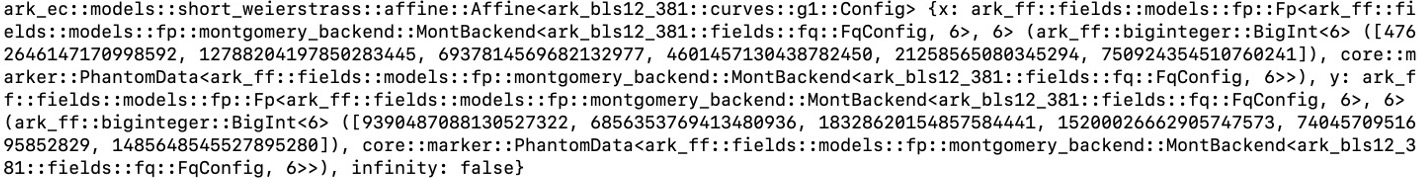
\includegraphics[width=\textwidth]{ch-snarkprobe/figure/prettyprint-c.jpg}
  \caption{Content without PrettyPrint in \arkworks}
  \label{subfig:snarkprobe-prettyprint_c}
\end{subfigure}
\par\vspace{10pt}
\begin{subfigure}{0.9\textwidth}
  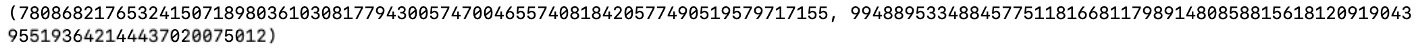
\includegraphics[width=\textwidth]{ch-snarkprobe/figure/prettyprint-d.jpg}
  \caption{Content with PrettyPrint in any library}
  \label{subfig:snarkprobe-prettyprint_d}
\end{subfigure}
\caption{Content of variable type G1}
\label{fig:snarkprobe-prettyprint}
\end{figure}



\parheadit{\valueextractor.}
The \valueextractor extracts all variables defined in the ideal value file using GDB and PrettyPrint.  As the ideal value file contains the line number where each variable is assigned, the \valueextractor can automatically set up a breakpoint for each variable immediately after its assignment. Then, when the input program reaches this, the \valueextractor uses PrettyPrint to save the variable's formatted value. %The program will continually run until all GDB breakpoints have been hit and all variables' values have been saved.

\parheadit{\valuechecker.}
%\label{secsec:snarkprobe-impvaluechecker}
We developed the \valuechecker for \pinocchio by following \cite{parno2013pinocchio} and \cite{ben2014succinct} and \groth16 by \cite{groth2016size} and \cite{nitulescu2020zk}. To help ensure accurate re-evaluation of the protocol calculations, the \valuechecker uses exactly the same variable names as the original papers, and we follow the protocol description exactly, without any optimizations, to avoid introducing mistakes.

\parheadit{ECC Libraries.} We use two well-tested elliptic curve libraries to demonstrate diversity and flexibility.
py\_ecc \cite{pyecc}, developed by Ethereum in Python, supports both the BN128 and BLS12-381 curves. CIRCL \cite{circl}, developed by Cloudflare in Go, supports BLS12-381.  Since it is written in Go, we developed the necessary APIs so that our Python-based \valuechecker can access the functions. If users would like to test a new zkSNARK library using a curve that py\_ecc or CIRCL do not support, they can easily plug it into the \valuechecker in this same manner.

%%%%%%%%%%


\subsubsection*{\underline{\SnarkFuzzer: \valuemonitor}}
\label{subsec:snarkprobe-value-monitor}

\textbf{Goals: } \emph{The \valuemonitor detects any unexpected value changes after the extraction of initial variable values from the source program.}

\parhead{Design.}%
While the \valuemodel extracts all necessary variables' values at the location where the variables are first assigned, and we also need to check if there is a value change after the model extracts these values to ensure consistency between the library and the \valuechecker. The \valuemonitor can also detect any unexpected side effects caused by the library or dependent functions due to incorrect implementation, out of memory, or other unexpected errors.

\parhead{Implementation.}%
GDB watch allows \SnarkFuzzer to monitor value changes in a debugging session with four CPU debug registers called hardware watchpoints. A hardware watchpoint is very efficient, but it does not support larger data structures given the limited debug registers. Software watchpoints will be automatically applied if GDB tries to setup a watchpoint for a variable that cannot be handled by a hardware watchpoint. Unlike hardware watchpoints, software watchpoints are extremely slow, and watching dozens of variables may require unacceptable processing time. For example, using GDB software watch for a single variable \texttt{A\_query} in \libsnark takes more than 30 minutes.

Therefore, we instead used Valgrind, a dynamic analysis tool that analyzes a program to automatically detect memory management and threading bugs. Valgrind has a gdbserver to simulate traditional GDB hardware watchpoints. Simulation still takes longer than pure GDB hardware watchpoints, but the hardware watchpoint simulation is much faster than GDB software watchpoints. Meanwhile, Valgrind hardware watchpoint simulation does not have any limitation on the number and length of variables, so Valgrind can be used for any zkSNARK source program and libraries with complex data structures.
\section{Performance Evaluation}
\label{sec:snarkprobe-evaluation}

Our first set of evaluations for \tool explores its performance and scalability.
All experiments run on an Intel Core i7-8700 CPU @ 3.20\,GHz $\times$ 12 with 32\,GB of RAM running 64-bit Ubuntu 22.04 LTS.

\subsection{Performance of the \ConstraintChecker}
We start by testing the \ConstraintChecker and evaluate its performance on statements with different types of operations and complexities, and present the runtimes in Table \ref{tab:snarkprobe-performance1}.
There are two runtime results for each experiment.  We first recorded the runtime for the SMT solver, which is the most important step in the \ConstraintChecker, and we also recorded the total runtime, including the processing time of the Circuit Extractor, SMT solver, and other internal evaluations.

We tested different types of proofs, including the well-known cube example, a comparison (which requires using a gadget), a hash (a complicated mathematics equation), and a proof with inner product, logical operators, and comparison (which requires multiple gadgets and more complex logic). As expected, as we progress in terms of ``complexity'', runtime generally increases.  Interestingly, the hash proof takes the longest in the SMT solver, demonstrating that there are different notions of ``complexity'' than just statement size.

%\clg{We observed that processing time is generally determined by the specific relations in circuit, which depends on the runtime to solve the equations by SMT solver. Interestingly, a large, ``complicated'' R1CS matrix or statement equation may not need a longer time to be evaluated by the \ConstraintChecker, since the ``complicated'' R1CS matrix may actually be easy for the SMT solver to handle.} \clg{Maybe remove this text since we don't have any way to back it up or justify it?} 

We also sought to test if the correctness of the statement checked had any impact on performance.  We did this by running two different experiments with the cube proof, one where we model a developer correctly flattening the statement equation into R1CS, and a second where we model a mistake in the flattening that introduces an error. Our \ConstraintChecker took a shorter time to evaluate the incorrect cube program since the \ConstraintChecker aborts as soon as it finds an error (such as a different domain or output value). 

\begin{table}[t]
\centering
\begin{adjustbox}{max width=\textwidth}
\begin{tabular}{c|c|cc}
\hline
\multirow{2}{*}{Statement} & \multirow{2}{*}{Equation} & \multicolumn{2}{c}{Runtime (in seconds)} \\ \cline{3-4} 
                           &                           & \multicolumn{1}{c|}{SMT Solver}     & Overall    \\ \hline\hline
Cube                       & $y = x^3 + x + 5$         & \multicolumn{1}{c|}{0.49}           & 4.18       \\ \hline
Cube with Error            & $y = x^3 + x + 5$         & \multicolumn{1}{c|}{0.24}           & 3.94       \\ \hline
Comparison                 & $x < 60$                  & \multicolumn{1}{c|}{0.54}           & 12.39      \\ \hline
SHA-256 Hash               & $y = \texttt{sha256}(x)$    & \multicolumn{1}{c|}{0.71}           & 15.39      \\ \hline
Inner Product        & $\langle u,v \rangle < c_1 \land \langle u,v \rangle > c_2$ & \multicolumn{1}{c|}{0.59}           & 18.34      \\ \hline
\end{tabular}
\end{adjustbox}
\caption{\ConstraintChecker runtime for different proof statements}
\label{tab:snarkprobe-performance1}
\vspace*{-20pt}
\end{table}

%%%%%%%%%

\subsection{Performance of \SnarkFuzzer}
\label{subsec:snarkprobe-performance-fuzzer}

We tested \SnarkFuzzer on \libsnark, \bellman, \arkworks, and \gnark to evaluate the processing time and performance in different configurations.
All experiments run on a single core, except for the \valuemonitor which is trivially parallelizable across all cores.
We start by evaluating the overall tool to examine the runtime percentage that is dedicated to each sub-component.  We then drill down and individually explore the scalability of each sub-component to gain a fuller understanding of \SnarkFuzzer's overall scalability. % We discuss the most influential performance results here, and provide additional benchmarks in Appendix~\ref{app:additionalgraphs}.

%%%%%

\parhead{Overall Runtime with Different Libraries and Protocols.}
We first explore the proportion of total running time that each different facet of \SnarkFuzzer takes, and present the results in Figure~\ref{fig:snarkprobe-time}.

We ran with five different configurations: \libsnark with \pinocchio, \libsnark with \groth16, \bellman with \groth16, \arkworks with \groth16, and \gnark with \groth16. All of these experiments use generation-based fuzzers to produce valid R1CS matrices (the slowest of the four fuzzing methods we provide) with dimensions in $[30,60]$.  We ran 30 iterations of the \branchmodel (since as shown in Figure~\ref{fig:snarkprobe-coverage} that provides reasonable coverage) and calculated the average runtime to complete a full ``run''\footnote{We define a ``full run'' to be using the \inputgenerator to produce one zkSNARK program, analyzing coverage status with the \branchmodel, and looking for any software and cryptographic related bugs with the \valuemodel and \valuemonitor.} and proof check for each library and protocol.

\begin{figure}[t]
  \centering
  %\captionsetup{justification=centering}
  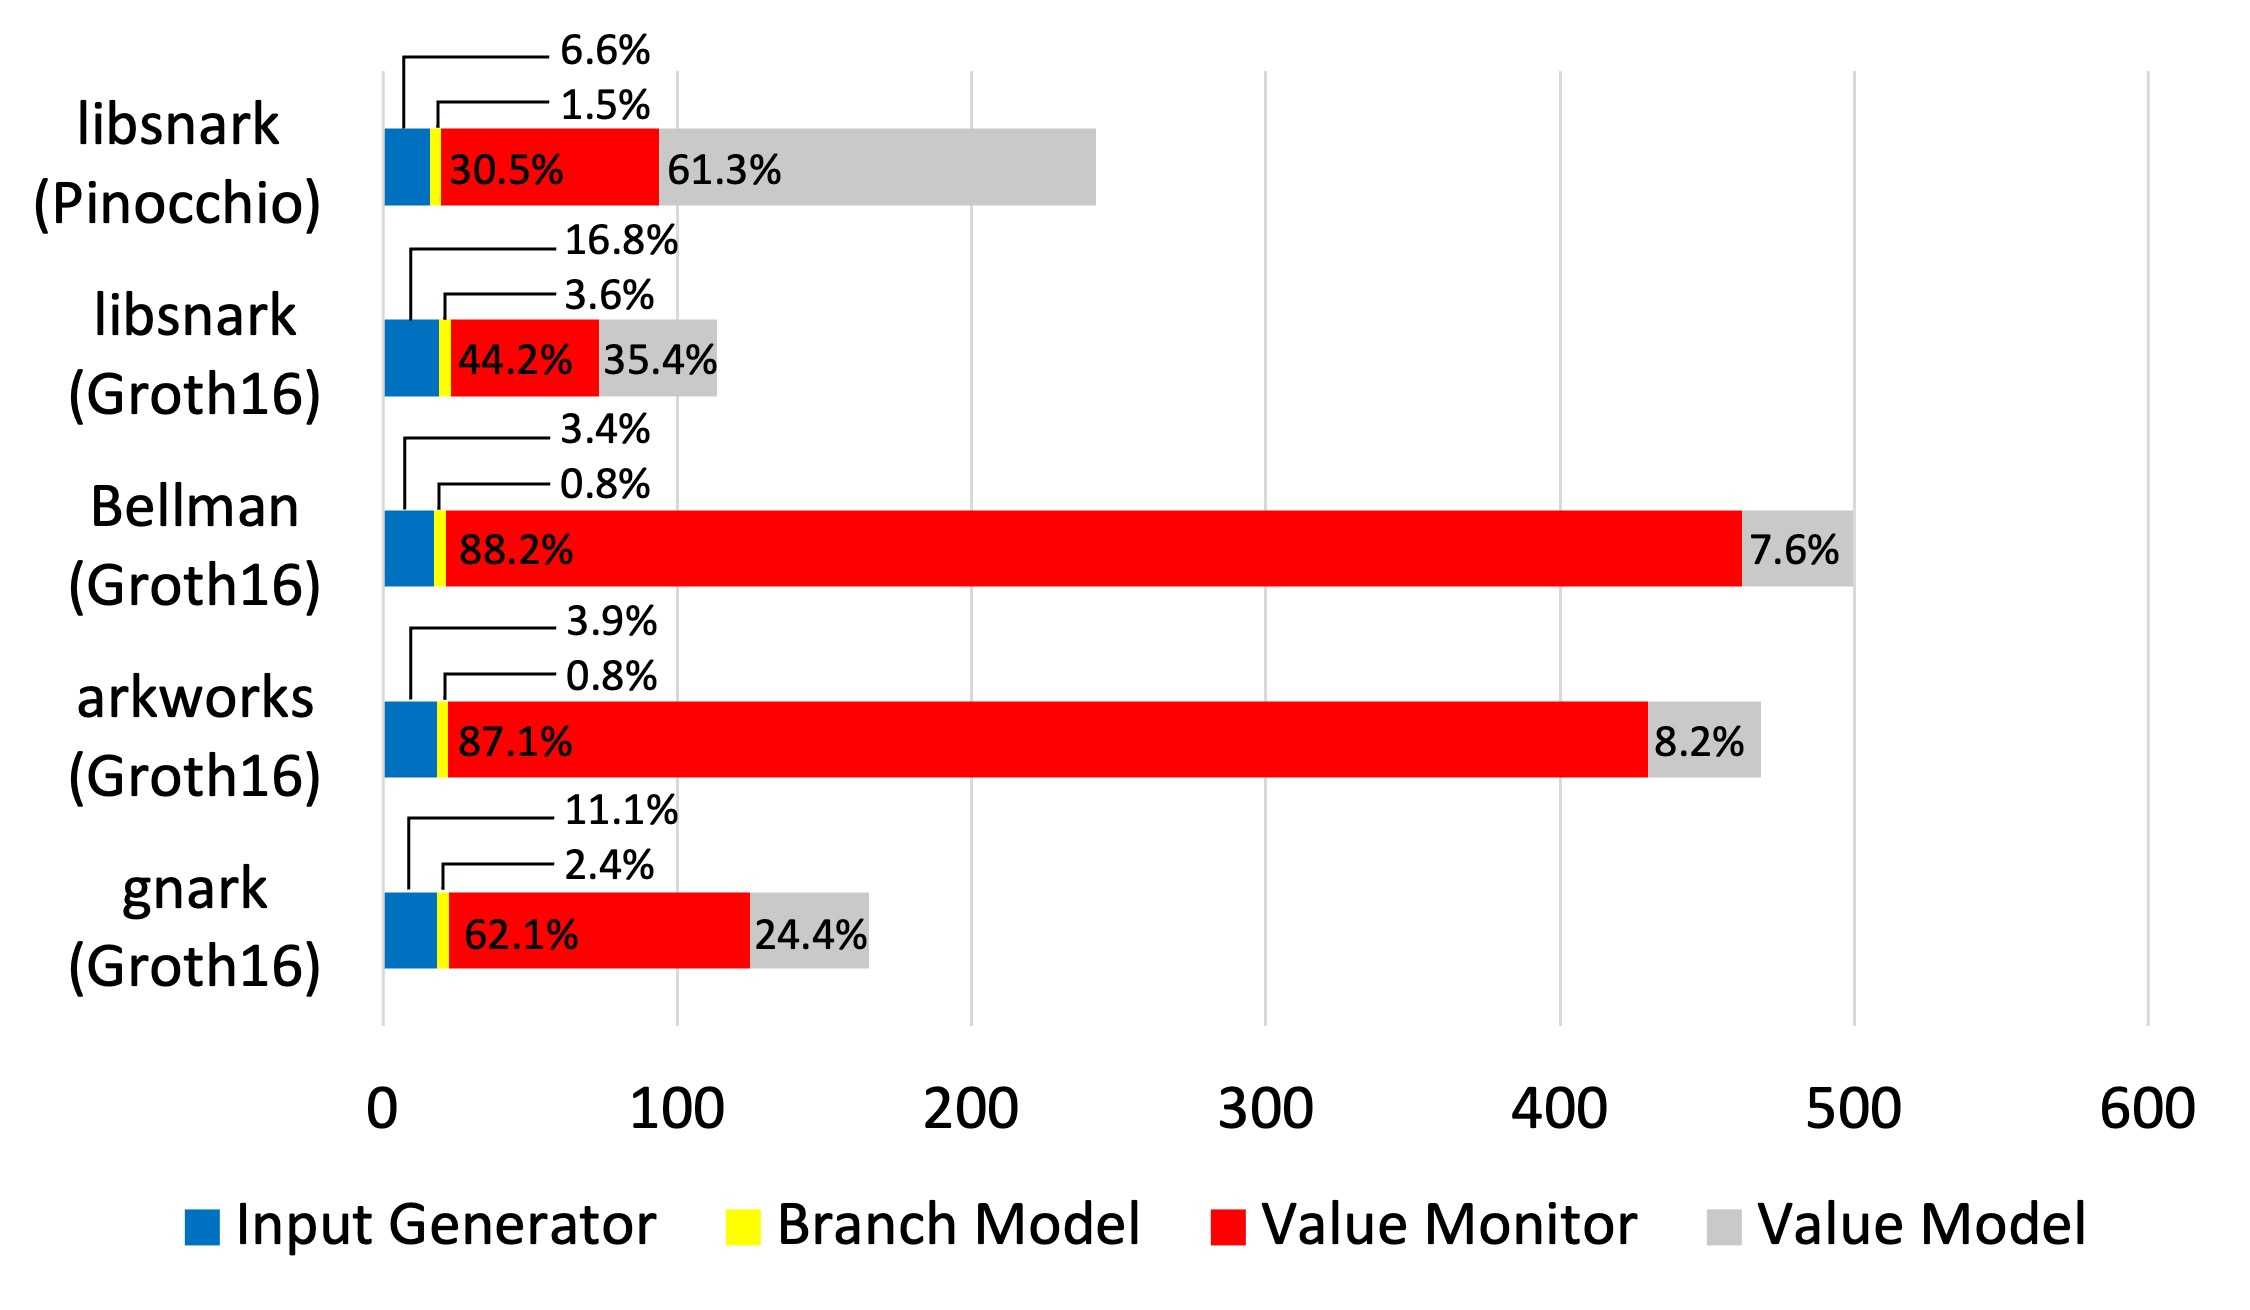
\includegraphics[width=0.8\linewidth]{ch-snarkprobe/figure/time.jpg}
	\vspace*{-10pt}
  \caption{Runtime of each component in \SnarkFuzzer with different libraries and protocols, both in terms of actual time as well as percentage of the total.}
  \label{fig:snarkprobe-time}
\vspace*{-10pt}
\end{figure}

%As we can see, the overall runtime is reasonable even in this slowest configuration, taking roughly 280 seconds for \libsnark with \pinocchio, 130 seconds for \libsnark with \groth16, and 580 seconds for \bellman with \groth16 to complete a full ``run''\footnote{We define a ``full run'' to be using the \inputgenerator to produce one zkSNARK program, analyzing coverage status with the \branchmodel, and looking for any software and cryptographic related bugs with the \valuemodel and \valuemonitor.} and proof check.

We observe that for all libraries and protocols, the majority of time is spent in the \valuemonitor and \valuemodel phases.  This is somewhat expected, as the cryptographic operations in the \valuemodel require time to calculate, and Valgrind's simulation hardware watch also introduces substantial overhead.  Since \groth16 has fewer elliptic curve and pairing operations than \pinocchio, testing that involves \groth16 costs less time. However, Valgrind spends a longer time executing a program in Rust than a program in C and Go. Since we use Valgrind in the \valuemonitor to find and monitor value changes, we see a longer overall runtime with \bellman and \arkworks than \libsnark and \gnark.

We do use small R1CS matrices in these experiments, as the primary goal is to demonstrate the runtime proportion for each component.  We make a few key observations about this.  We noticed that unless one uses only generation-based fuzzing to produce valid inputs, the size of the R1CS matrix (i.e., the proof) will not substantially affect the performance of the \inputgenerator.  The \branchmodel does not work with the R1CS matrix, so different sizes will result in the same runtime.
However, a large matrix will significantly increase the runtime of the \valuemodel and \valuemonitor (see Table~\ref{tab:snarkprobe-performance2} for more realistic values).  For total runtime reference, an R1CS matrix of size $100 \times 5000$ takes about 940 seconds to run the complete \SnarkFuzzer with our generation-based invalid matrix fuzzer.

%As we discussed previously, we are enable to trivially enable parallel running for the \valuemonitor across multiple CPU cores to reduce its percentage of processing time.  This is because the \valuemonitor watches all variables defined in the ideal value file, and unlike the \valuemodel, watching a single variable does not require communication with any other variables that need to be watched.

%We note that there are a number of avenues for optimization that would decrease the overall runtime.
%Switching to a different mechanism for the \valuemonitor could also decrease performance as well, and we will discuss the performance improvement in Section \ref{subsubsec:scalability}.

%%%%%


\parhead{Performance of the \inputgenerator.}
Unlike a mutation-based or generation-based fuzzer for an invalid matrix (which are very quick since they only require straightforward operations), generating a valid R1CS matrix with our generation-based fuzzer requires the SMT solver to produce a matrix based on the random witness array. Thus the processing time depends on the matrix size and random value(s) in the witness list, which generally results in a larger matrix taking longer to process.
To validate this, we used our various fuzzers to produce matrices of varying sizes (remember that the rows represent the number of constraints and columns the number of variables). In Table \ref{tab:snarkprobe-gen-invalid}, we present the processing time for each method (generally under one second for most methods), which confirms our general intuition.
We also note that the \inputgenerator must compile the input matrix (proof) and source code into a binary program, which can require substantial time that is outside of our control.
%Some \zksnark libraries may require longer compiling time, and we have no control to the library compiling time cost, which will increase our \inputgenerator total runtime.
%\delete{ Although a larger matrix usually takes a longer time to generate, a ``smaller'' R1CS matrix may also require greater computational resources depending on the random numbers chosen in the witness and R1CS relations, as this can cause simplified relations in R1CS matrix and witness, thus requiring the SMT solver to take less time to calculate a valid R1CS matrix.\yuquan{Might need better explanation for this line?}  For example, we can see that matrix three and matrix seven in the 10 × 200 category only take roughly ten seconds to generate, which is similar to generating a matrix of size 20 × 40.} \fanyo{(summary)}

%\begin{figure}[t]
  %\centering
  %%\captionsetup{justification=centering}
  %\includegraphics[width=0.9\linewidth]{imgs/gen-invalid.jpg}
  %\caption{Runtime of the \inputgenerator to produce R1CS matrices of different sizes.}
  %\label{fig:snarkprobe-gen-invalid}
%\end{figure}

\begin{table}[h]
\centering
\begin{adjustbox}{max width=\textwidth}
\begin{tabular}{ll||c|c|c|c}
\hline
\multicolumn{2}{l||}{Matrix Size} & $5 \times 10$ & $20 \times 40$ & $50 \times 100$ & $50 \times 200$ \\ \hline\hline
\multicolumn{1}{l||}{\multirow{2}{*}{}Generation Based} & Invalid Matrix & \textless{}0.01 & \textless{}0.01 & \textless{}0.01 & 0.02 \\ \cline{2-6}
\multicolumn{1}{l||}{} & Valid Matrix & 0.16 & 2.06 & 23.02 & 51.27 \\ \hline
\multicolumn{1}{l||}{\multirow{2}{*}{}Mutation Based} & Invalid Matrix & 0.38 & 0.49 & 0.65 & 0.77 \\ \cline{2-6}
\multicolumn{1}{l||}{} & Valid Matrix & \textless{}0.01 & \textless{}0.01 & \textless{}0.01 & 0.02 \\ \hline
\end{tabular}
\end{adjustbox}
\caption{Runtime (in seconds) of the \inputgenerator to produce R1CS matrices of different sizes.}
\label{tab:snarkprobe-gen-invalid}
% \vspace*{-14pt}
\end{table}

%%%%

\parhead{Performance of the \branchmodel.}
Next, we explore the coverage ability of the \branchmodel in terms of breadth, as well as how quickly we achieve a high percentage of branch coverage.  We ran 50 iterations of the \branchmodel with \libsnark, which covers more than 85\% of all branches.  We stopped our experiments after 50 iterations as \SnarkFuzzer did not reach any new branches over the previous 10 prior iterations.  Even with this, we note that after roughly 30 iterations we see the breadth of our coverage begin to taper off.
A graph can be found in Figure \ref{fig:snarkprobe-coverage}.
%\fanyo{Even the \tool have covered most pf the branches in the target libraries, the fuzzer should not be stopped in order to generate more different inputs to test a same branch. The fuzzer should not be stopped until most of the branches have been tested for at least one time. As more inputs are generated, \tool has higher chance to find the potential issues in the target library or higher confidence to say (need a better word) that the target library is safe. }
%There are a number of factors that can affect our coverage results. First, we can encounter situations where the generation-based fuzzer cannot produce enough diverse input sets to cover all branches, which is where the seeds of the mutation-based fuzzer can play an important role in coverage.  Second, \SnarkFuzzer allows a user to configure the proportion of matrices generated by each sub-fuzzing method, which can also affect the coverage result. In our experiment, we had the generation-based fuzzer produce 5\% invalid and 45\% valid matrices, and the mutation-based fuzzer produce 40\% invalid and 10\% valid matrices. Increasing the fuzzing time and/or adding extra seeds for the mutation-based fuzzer can improve the coverage of a target source library.

\begin{figure}[h]
  \centering
  %\captionsetup{justification=centering}
  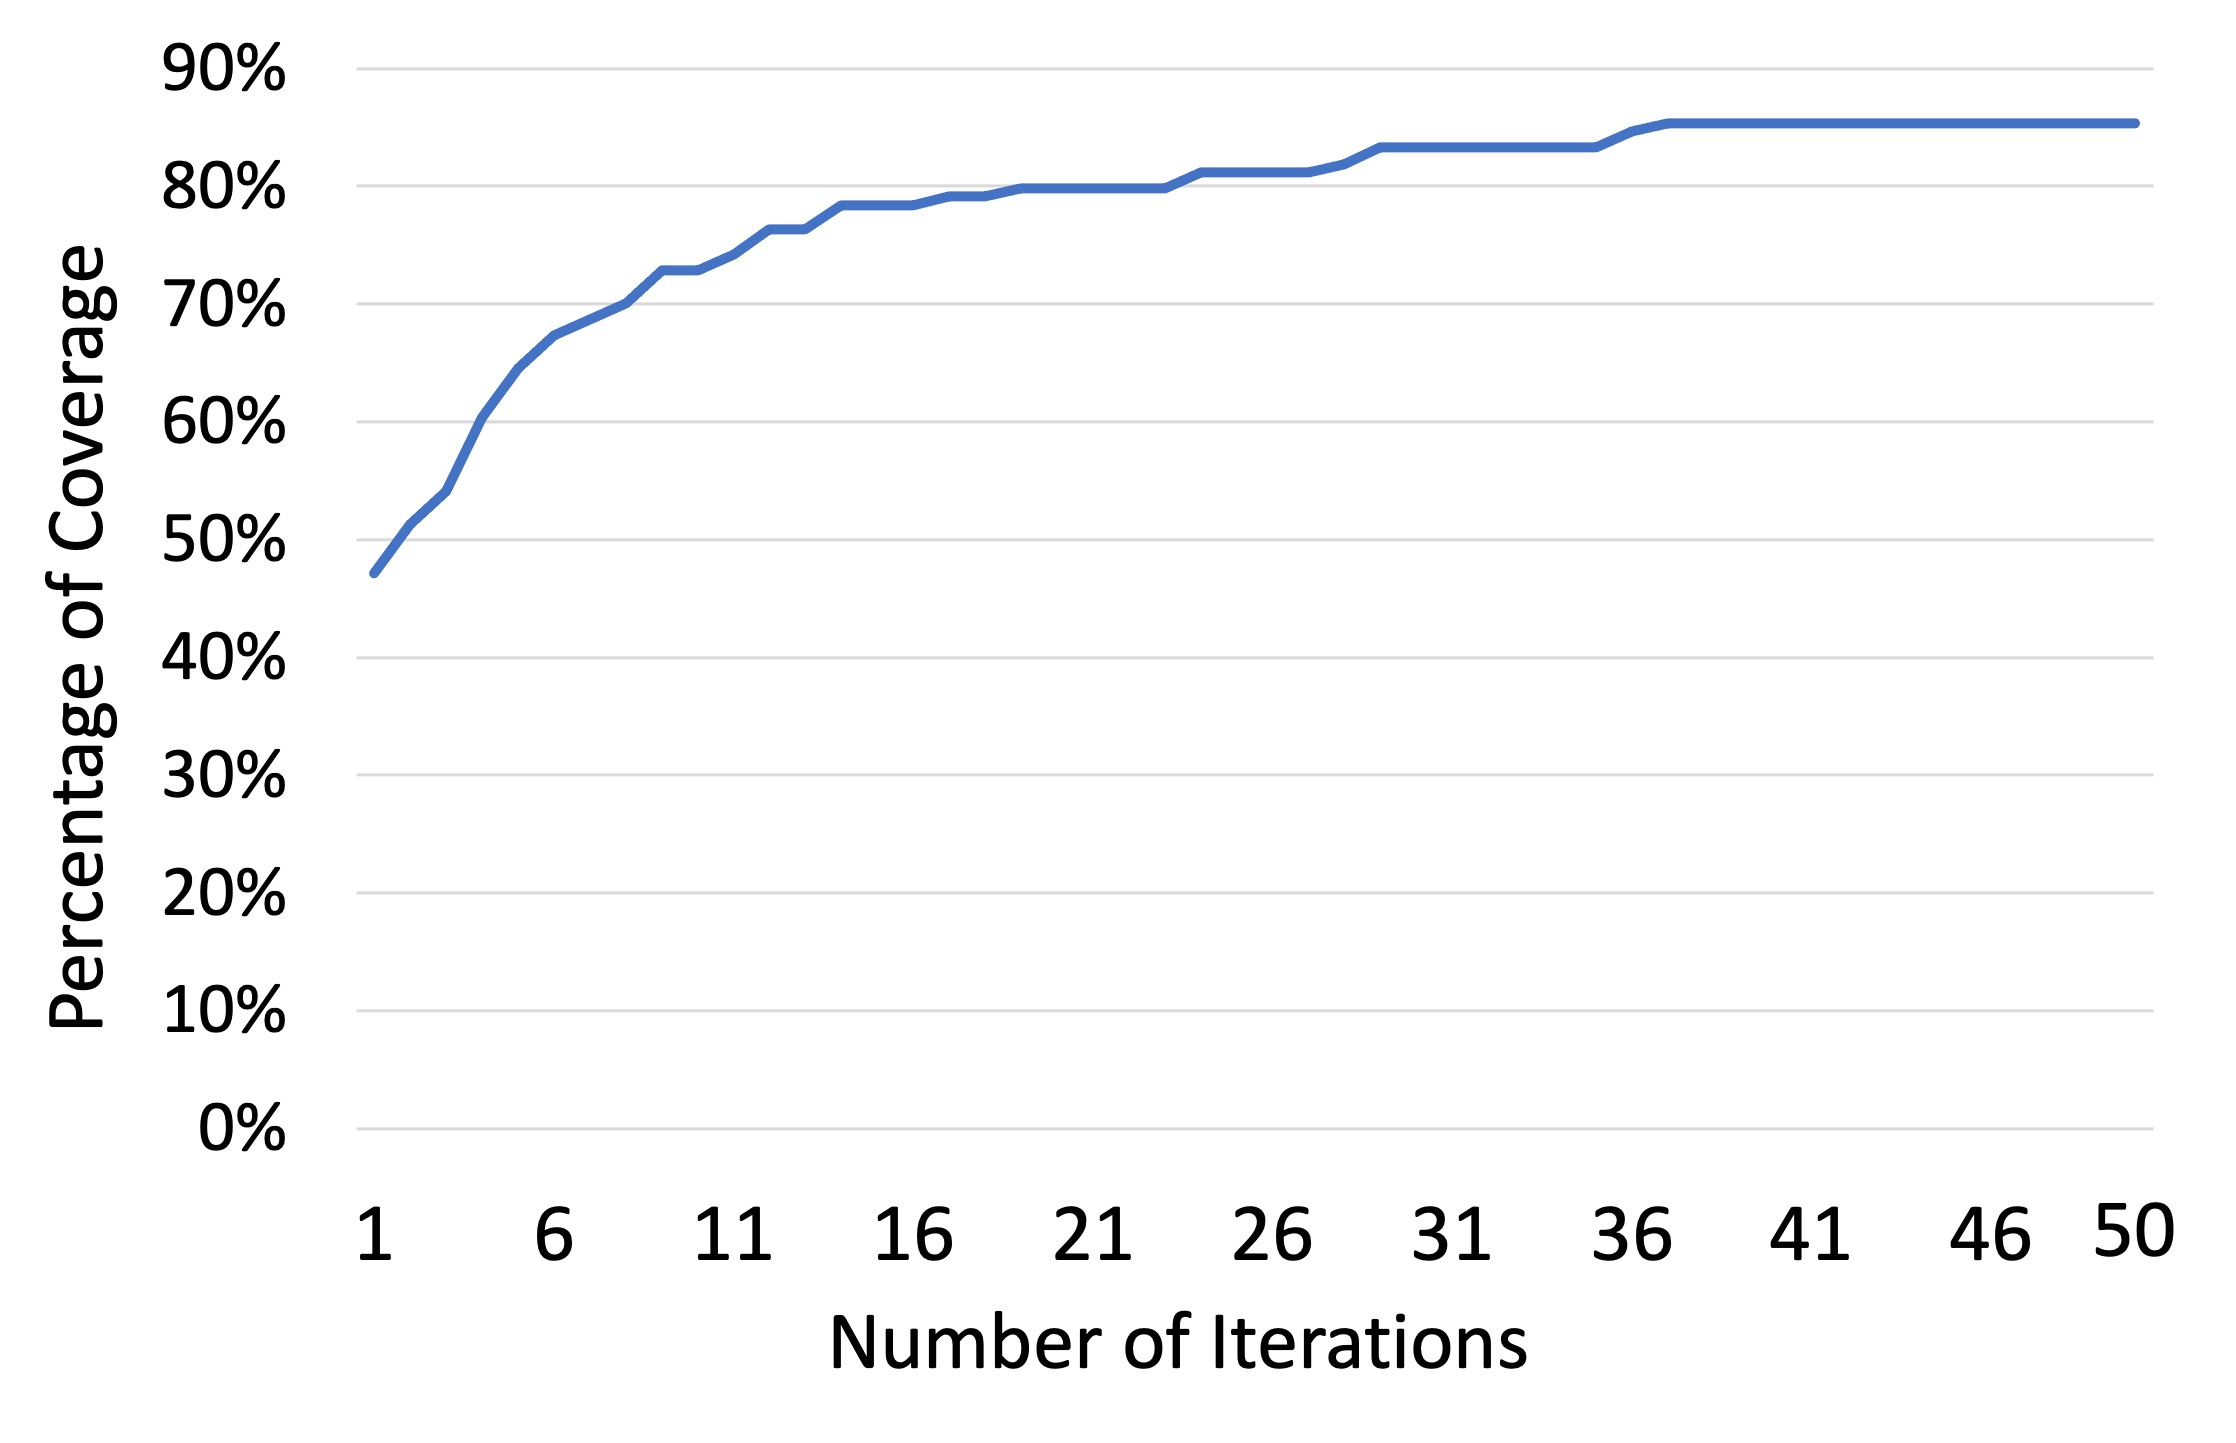
\includegraphics[width=0.70\linewidth]{ch-snarkprobe/figure/coverage.jpg}
  \vspace*{-10pt}
  \caption{Percentage (breadth) of library coverage after a given number of iterations}
  \label{fig:snarkprobe-coverage}
  %\vspace*{-8pt}
\end{figure}

%%%%%%%%%%


\parhead{Performance of \valuemodel and \valuemonitor.}
The primary effects on overall performance are our \valuemodel and \valuemonitor.  Table \ref{tab:snarkprobe-performance2} shows the runtime with different matrix sizes.  We expect the size of our matrices to be one of the primary influences on the runtime of these components.

Recall that the computation of the proving key requires calculations with the circuit.
%, such as \[ pk_A := \{A_{i}(\tau)\alpha_{A}\rho_{A}\mathcal{P}\}_{i=0}^{m+3} \] in \pinocchio protocol \cite{ben2014succinct} and \[ v(x) = \sum_{k=0}^{m} a_{k} v_{k} (x) \] in \groth16 protocol \cite{nitulescu2020zk}.
Therefore, a larger R1CS matrix will result in longer runtime in our \valuemodel. At the same time, the shape of the matrix will also affect its runtime. As we can see in Table \ref{tab:snarkprobe-performance2}, a matrix of size $20 \times 45$ takes less time than one of size $30 \times 30$ or $45 \times 20$, even though they all contain 900 integers. In fact, the number of variables (columns) plays a greater role than the number of constraints (rows) in \valuemodel runtime, since this plays a larger role in the size of the proving and verification keys. %For example, a matrix of size 45 × 20 has fewer integers than a matrix of size 45 × 60, but the \valuemodel spends similar runtime (around 41 seconds) to re-evaluate the programs with these two matrices. \yuquan{If we are showing that number of columns has greater influnece on runtime than number of rows, I think a comparison between 20 × 45 (29.52s) and 60 × 45 (46.03s) makes more sense? Maybe just add "In contrast, the Value Model runtime difference between 20 × 45 matrix and 60 × 45 matrix reaches 16.51 seconds."}

Similarly, the \valuemonitor requires more time to watch variables in a program with a larger matrix. However, the reason for this is different.  Since the runtime of Valgrind depends on the space complexity of a variable, the matrix shape will not have an effect. Instead, the \valuemonitor spends more time monitoring a program with a larger matrix, but it takes similar time for programs with the same number of integers but different shapes.  For example, each matrix of size $20 \times 45$, $30 \times 30$, and $45 \times 20$ has 900 integers, and the \valuemonitor takes around 46 seconds to run, even though they have a different shape.

\begin{table}[t]
\centering
\begin{adjustbox}{max width=\textwidth}
\begin{tabular}{cc||cc}
\hline
\multicolumn{2}{c||}{Matrix Setting} & \multicolumn{2}{c}{Processing Time (in second)} \\ \hline
\multicolumn{1}{c|}{Matrix Size} & Items in Matrix & \multicolumn{1}{c|}{\valuemodel} & \valuemonitor \\ \hline\hline
\multicolumn{1}{c|}{$10 \times 30$} & 100 & \multicolumn{1}{c|}{23.33} & 29.21 \\ \hline
\multicolumn{1}{c|}{$10 \times 30$} & \multirow{2}{*}{300} & \multicolumn{1}{c|}{25.96} & 33.09 \\ \cline{1-1} \cline{3-4} 
\multicolumn{1}{c|}{$30 \times 10$} &  & \multicolumn{1}{c|}{32.78} & 34.21 \\ \hline
\multicolumn{1}{c|}{$20 \times 45$} & \multirow{3}{*}{900} & \multicolumn{1}{c|}{29.52} & 43.99 \\ \cline{1-1} \cline{3-4} 
\multicolumn{1}{c|}{$30 \times 30$} &  & \multicolumn{1}{c|}{33.01} & 46.30 \\ \cline{1-1} \cline{3-4} 
\multicolumn{1}{c|}{$45 \times 20$} &  & \multicolumn{1}{c|}{40.14} & 47.68 \\ \hline
\multicolumn{1}{c|}{$45 \times 60$} & \multirow{2}{*}{2700} & \multicolumn{1}{c|}{41.29} & 81.69 \\ \cline{1-1} \cline{3-4} 
\multicolumn{1}{c|}{$60 \times 45$} &  & \multicolumn{1}{c|}{46.03} & 80.21 \\ \hline
\multicolumn{1}{c|}{$100 \times 1500$} & 150000 & \multicolumn{1}{c|}{200.84} & 223.49 \\ \hline
\multicolumn{1}{c|}{$100 \times 5000$} & 500000 & \multicolumn{1}{c|}{580.97} & 344.83 \\ \hline
\end{tabular}
\end{adjustbox}
\caption{Runtime of the \valuemodel and \valuemonitor to process an R1CS matrix of varying size.  For example, $10 \times 30$ is a matrix with 10 variables and 30 constraints.}
\label{tab:snarkprobe-performance2}
% \vspace*{-14pt}
\end{table}

\parhead{Discussion of Total Runtime.}
Our experiments only provide an upper bound on the worst case runtime for \SnarkFuzzer.  We did not perform any runtime optimizations, and in all of our experiments, we used the slowest options or configurations that we knew of.
While \SnarkFuzzer does require extra runtime in the \valuemonitor and \valuechecker for each individual input seed, in comparison to a traditional fuzzer, which might spend hundreds or thousands of core hours to produce inputs, the \framework and \branchmodel designs allow\SnarkFuzzer to find issues with a relatively small number of generated input seeds.
In fact, most errors that \SnarkFuzzer detected (see Section \ref{sec:snarkprobe-errorcatching}) were found with less than ten seeds.
Therefore, we view performance to be acceptable for real world usage.

%%%%%

\iffalse

\subsection{Scalability and Paths to Improvement}
\label{subsec:snarkprobe-scalability}

Finally, we conclude our performance evaluation with a brief discussion about the scalability of \SnarkFuzzer.
Our experiments only provide an upper bound on the worst case runtime for \SnarkFuzzer.  We did not enable or perform any runtime optimizations (except for parallel running in the \valuemonitor).  And in all of our experiments, we used the slowest options or configurations that we knew of (for example, we computed the overall tool runtime in Figure~\ref{fig:time} using the slowest of our fuzzing options).  We tested on a wide variety of R1CS matrix sizes and configurations, which are representative of statements of varying complexity (recall that the number of constraints in R1CS roughly maps to the number of gates in an arithmetic circuit).  In all of these instances, we view performance to be acceptable for real world usage, as nothing takes more than tens of minutes to run overall.

%we used z3py (a Z3 API in Python) to generate a valid R1CS matrix in the \inputgenerator because it was easy to use and integrated with our framework \clg{Why did we pick this one and not, say Z3, which is popular, again?}. Comparing with standard Z3 or other high performance theorem provers, z3py is especially slow at solving an equation with many variables.
However, there are several paths to reduce the processing time further.
For example, the \inputgenerator could be sped up by replacing z3py with another theorem prover in a lower level language or by new SMT solvers \cite{Parafrost-OsamaWB-tacas21, fpsmtgpu, osama2021gpu} that can be accelerated by a GPU.
For the \valuemonitor and \valuemodel, we note that our implementation choices can (easily) be replaced by other similar techniques to improve runtime. For example, when testing a library that does not contain any large data structures, GDB hardware watch might be the right choice to monitor variables instead of Valgrind, as this is extremely efficient (but can only watch a limited number of variables at a time). And the \valuechecker could be enhanced by parallelization, though one must be careful to handle core communication since some values must be calculated in a specific order.

\fi

%\begin{table}[h]
%\centering
%\begin{tabular}{|l|l|l|l|}
%\hline
%Library            & \multicolumn{2}{l|}{\libsnark} & \bellman \\ \hline
%Protocol           & PGHR13 & Groth16 & Groth16 \\ \hline
%Total Variables    & 78     & 44      &         \\ \hline
%Integer            & 6      & 1       &         \\ \hline
%Finite Field       & 12     & 6       &         \\ \hline
%G1                 & 20     & 13      &         \\ \hline
%G2                 & 14     & 11      &         \\ \hline
%Finite Field Array & 8      & 4       &         \\ \hline
%G1 Array           & 17     &         &         \\ \hline
%G2 Array           & 1      &         &         \\ \hline
%
%\end{tabular}
%\caption{Extractor}
%\label{tab:extractor}
%\end{table}

%%%%%%%%%%

\section{Error Catching Evaluation}
\label{sec:snarkprobe-errorcatching}

Our second set of evaluations demonstrates \tool's ability to \emph{automatically} catch different types of errors in \zksnark libraries.  We test \tool on \libsnark, \bellman, \arkworks, and \texttt{playsnark}, as well as on the circuit generator \circom.  Additionally, we show how \tool would have caught a previous CVE in the \zksnark component of Zcash, a popular privacy-preserving cryptocurrency.  In total, \tool detected seven inconsistencies in current \zksnark libraries, successfully \textit{automatically} located the previous vulnerability, and could potentially detect two additional types of errors. % (which we discuss in Appendix~\ref{app:potentialerrors} due to space constraints as these were not found in any high profile applications at this time). 
We summarize our results in Table~\ref{tab:snarkprobe-error_summary}.%, including the type of error, which component of \tool is able to detect the error, and what exactly the error affects.

%\fanyo{The main goals of our evaluations of \tool are to show that 1) out tools can detect errors or vulnerabilities especially \logicerror{} in \zksnark libraries with improved performance comparing to other tools; 2) our tools have can detect these errors in a reasonable runtime with real \zksnark libraries and applications.}

%\fanyo{Our first major point of evaluation is \tool's ability to \emph{automatically} catch different types of errors in widely-used zkSNARK libraries and circuit generator.  In this section, we introduce the errors that \tool found in real world \zksnark libraries for both \ConstraintChecker and \SnarkFuzzer. We also evaluate \SnarkFuzzer to compare with current fuzzing tool to show the performance improvements and enhanced abilities of our design. We will also discuss the runtime performance in Section \ref{sec:evaluation}.}
%
%\fanyo{We firstly evaluated \tool with three major, widely used \zksnark libraries and its circuit generator including \libsnark, \bellman, and \arkworks. Meanwhile, we also evaluate some other libraries and circuit generator from recent projects and academic papers such as playsnark, LegoSNARK, and Circom. To better show the ability of our \tool, we also evaluate our \tool with previous \zksnark library versions, and the evaluation results shows that our \tool can also detect. In total, \tool found 7 issues or bugs in current \zksnark libraries plus 1 vulnerability in previous version \zksnark library and table \ref{tab:error_summary} contains the summary information for each bug \tool found.}


\begin{table}[p]
\centering
\rotatebox{90}{
\begin{minipage}{\textheight}
\footnotesize
{
\renewcommand{\arraystretch}{1.5}
\begin{tabular*}{\textheight}{@{\extracolsep{\fill}}|lllll|}
\hline
\multicolumn{1}{|c||}{\textbf{Error/Vulnerability}} &
\multicolumn{1}{c|}{\textbf{Type}} &
\multicolumn{1}{c|}{\textbf{Affected Component}} &
\multicolumn{1}{c|}{\textbf{Program}} &
\multicolumn{1}{c|}{\textbf{Found by}} \\ \hline\hline

\multicolumn{5}{|c|}{\textit{Potentially Locatable in Current Libraries}} \\ \hline
\multicolumn{1}{|l||}{Incorrect manual flattening by developer} & \multicolumn{1}{l|}{Logic Error} & \multicolumn{1}{l|}{R1CS Circuit} & \multicolumn{1}{l|}{All libraries} & ConstraintChecker \\ \hline
\multicolumn{1}{|l||}{Multiple gadget misuse} & \multicolumn{1}{l|}{Logic Error} & \multicolumn{1}{l|}{R1CS Circuit} & \multicolumn{1}{l|}{All libraries} & ConstraintChecker \\ \hline

\multicolumn{5}{|c|}{\textit{Found in Current Libraries}} \\ \hline
\multicolumn{1}{|l||}{Incorrect bit/comparison gadget implementation} & \multicolumn{1}{l|}{Logic Error} & \multicolumn{1}{l|}{R1CS Circuit} & \multicolumn{1}{l|}{libsnark} & ConstraintChecker \\ \hline
\multicolumn{1}{|l||}{Mismatch in circuit generation and usage} & \multicolumn{1}{l|}{Logic Error} & \multicolumn{1}{l|}{R1CS Circuit} & \multicolumn{1}{l|}{All libraries} & ConstraintChecker \\ \hline
\multicolumn{1}{|l||}{Groth16 pre-pairing computation in Setup} & \multicolumn{1}{l|}{Logic Error} & \multicolumn{1}{l|}{Groth16 Protocol} & \multicolumn{1}{l|}{bellman/arkworks} & SnarkFuzzer \\ \hline
\multicolumn{1}{|l||}{Inconsistent QAP extension index usage} & \multicolumn{1}{l|}{Logic Error} & \multicolumn{1}{l|}{PGHR13 Protocol} & \multicolumn{1}{l|}{libsnark} & SnarkFuzzer \\ \hline
\multicolumn{1}{|l||}{Toxic waste not safely destroyed} & \multicolumn{1}{l|}{Logic Error} & \multicolumn{1}{l|}{PGHR13 Protocol} & \multicolumn{1}{l|}{playsnark} & SnarkFuzzer \\ \hline
\multicolumn{1}{|l||}{Program out of memory with large circuit} & \multicolumn{1}{l|}{Software Error} & \multicolumn{1}{l|}{-} & \multicolumn{1}{l|}{libsnark} & SnarkFuzzer \\ \hline

\multicolumn{5}{|c|}{\textit{Found in Previous Versions of Libraries}} \\ \hline
\multicolumn{1}{|l||}{CVE-2019-7167} & \multicolumn{1}{l|}{Logic Error} & \multicolumn{1}{l|}{PGHR13 Protocol} & \multicolumn{1}{l|}{libsnark (2018)} & SnarkFuzzer \\ \hline
\end{tabular*}
}
\caption{Summary of the current potential errors and inconsistencies, and previous vulnerabilities, that \tool is able to catch and locate.}
\label{tab:snarkprobe-error_summary}
\end{minipage}
}
\end{table}



\subsection{Potentially Locatable in Current Libraries}
\parhead{Incorrect Flattening.}
There is always a possibility that a developer may generate an incorrect R1CS matrix for their circuit, since this process is often done by hand.
While we did not find any examples of this in the few applications we tested, consider the following scenario.
Take a statement equation like $x^3 + x + 5 = y$ which the developer will typically flatten into \texttt{R1CS\_gates} with private input $x = 3$ and public input $y = 35$.  This set of equations is then equal to $x^3 + x + 5 = 35$. However, the developer \emph{may} incorrectly flatten the statement equation into \texttt{R1CS\_gates\_2}.

% \vspace*{-6pt}
\noindent\begin{minipage}{0.5\linewidth}
{\small
\[ \texttt{R1CS\_gates} =
\begin{cases}
x * x = w_{1} \\
w_{1} * x = w_{2} \\
w_{2} + x = w_{3} \\
w_{3} + 5 = y
\end{cases} \]
}
\end{minipage}%
\begin{minipage}{0.5\linewidth}
{\small
\[ \texttt{R1CS\_gates\_2} := \begin{cases} 
x * x = w_{1} \\
w_{1} * x = w_{2} \\
w_{2} + 2 * x = w_{3} \\
w_{3} + 2 = y
\end{cases} \]
}
\end{minipage}
%\vspace*{-6pt}

While \texttt{R1CS\_gates\_2} still satisfies the private input $x = 3$ and public input $y = 35$, causing the underlying library to output an acceptable proof, this flattening does not in fact equal the statement equation $x^3 + x + 5 = y$.
Although the statement equation and \texttt{R1CS\_gates\_2} satisfy the witness, and their domains have the same upper and lower bounds, they have a different output range, which our \ConstraintChecker will catch and flag as an error.

\parhead{Combining Multiple Gadgets.}
%Many zkSNARK libraries provide an abstraction called a gadget to make realizing proofs easier for developers (see Section~\ref{sec:background}).
%Since manually flattening statement equations can be difficult in most real world examples, and many types of statements are often reused, gadgets are widely used by developers.  In fact, many existing libraries also recommend to newcomers in their tutorials that they use gadgets~\cite{arkworks}.
Recall that a gadget is an abstraction that many \zksnark libraries contain to make developing proofs easier for developers.
Multiple gadgets may also be combined to create a single proof.  Gadgets are generally created and provided independently, which means that one must combine them with care. For example, say a developer uses the gadgets $greater\_than$ and $equal\_to$ to create a proof that a prover has a value which is greater than or equal to a certain number.  For this proof, only one input should be used for both gadgets.  However, a naive developer may create a proof that has an individual input for each gadget instead of a single input for the entire circuit.  In this case, a malicious prover can create a separate program with the same circuit and use two inputs with different values to satisfy each gadget and hence the entire circuit (when in reality these two inputs need to be identical). In this case, our \ConstraintChecker can detect the inconsistency between the R1CS matrix and statement equations to find potential issues with using multiple gadgets incorrectly. 


\subsection{Found in Current Libraries}
\parhead{Defective Gadgets.}
%Many zkSNARK libraries provide an abstraction called a gadget to make realizing proofs easier for developers (see Section~\ref{sec:background}).
%Since manually flattening statement equations can be difficult in most real world examples (see Appendix~\ref{app:potentialerrors} for an example), and many types of statements are often reused, gadgets are widely used by developers.  In fact, many existing libraries also recommend to newcomers in their tutorials that they use gadgets~\cite{arkworks}.
Gadgets may be implemented incorrectly, causing inconsistencies between the original (desired) statement equation and the R1CS gates generated. Our \ConstraintChecker is able to find these inconsistencies in its checks for equivalence, regardless of whether a gadget was used or not. %The \ConstraintChecker found two different types of potential gadget issues in \libsnark.  While neither of these issues are critical flaws, and both can be prevented by a conscientious developer, it is good for even an experienced developer to be aware of potential implementation pitfalls and what is (and is not) handled by a library.
%\fanyo{Some gadgets in \libsnark require the developer to provide the size in bits of the integer value(s) in their proof. If an incorrect bit size is provided, then one can build a ``fake proof''\footnote{One that will verify even though the prover does not actually have a valid witness.}, and \libsnark will not block this behavior nor raise any warning messages to the verifier or implementer. A concrete example located by our \ConstraintChecker can be found in the \texttt{comparison\_gadget}. (delete)}

The \texttt{comparison\_gadget} in \libsnark uses bit shifting to compare two variables $A$ and $B$ by calculating $2^n + B - A$ and then counting the number of 0s and 1s in the resulting bit array (the corresponding R1CS constraints are shown in Appendix \ref{app:snarkprobe-comparison}). If the developer incorrectly specifies a bit length smaller than the size of $A$ or $B$, the \texttt{comparison\_gadget} will not generate the correct R1CS, which may result in a ``fake proof''\footnote{One that will verify even though the prover does not actually have a valid witness.}.  \libsnark will not block this behavior or raise any warning messages. Consider a developer that uses the \texttt{comparison\_gadget} to generate the statement equation $x < 60$ where $x \in \mathbb F_{p}$.  The R1CS should then only have a valid solution in $[0, 60)$. However, if an incorrect bit length is provided, we found that all numbers in the range $(\seqsplit{21888242871839275222246405745257275088548364400416034343698204186575808494653}, p)$ still satisfy this incorrect R1CS, allowing a dishonest prover to generate a valid proof without knowledge of a correct secret value.
After our tool flagged this potential issue, on further manual investigation we did see that the \libsnark source code contains a comment about using the correct bit size, though this could go unnoticed by a novice user or be abused by a malicious one to forge proofs.

%Since manually flattening statement equations can be difficult in most real world examples, and many types of statements are often reused, gadgets are widely used by developers.  Many existing libraries also recommend to newcomers in their tutorials that they use gadgets~\cite{arkworks}.  Because of this widespread usage, we feel that developers need to be aware of gadget subtleties, and as such \SnarkFuzzer can help increase the security of zkSNARK deployments.

\parhead{Mismatch Between Circuit Generation and Usage.}
In addition to end-to-end libraries, there are a growing number of circuit generators available to assist developers in constructing R1CS/circuits for proof generation, with \circom~\cite{circom} being a widespread example\footnote{We note that \circom is just an example that we tested, and that the same should hold true for other circuit generators as well.}.
\circom generates R1CS files that can then be utilized by libraries such as \texttt{snarkjs}~\cite{snarkjs}, \texttt{wasmsnark}~\cite{wasmsnark}, and \texttt{rapidSnark}~\cite{rapidsnark}. However, during our evaluation process, our \ConstraintChecker identified a crucial potential issue: the absence of attribute cross-checking between the circuit generator and formal proof generation library.

While the circuit generator may produce valid R1CS that accurately represents the prover's original statement, the proof generation library might, for example, employ a different elliptic curve and finite field to generate the proof by default. Consequently, when operating under distinct elliptic curve and finite field settings, the circuit no longer maintains equivalence with the original statement. This discrepancy can be problematic both for a developer and a verifier who are unaware that a circuit can yield different representations under different elliptic curve configurations.  In such cases, the prover can produce a seemingly ``valid'' proof for the verifier without knowledge of the secret value.


\parhead{\groth16 Pre-Pairing.}
The \groth16 protocol produces $P = g^{\alpha}$ and $Q = h^{\beta}$ as part of \textsf{Setup}, which are subsequently used in \textsf{Verify} to calculate the pairing $e(P, Q)$. However, our \valuechecker found that \bellman stores the pairing $e(P, Q)$ as part of the verification key instead of $P$ and $Q$. Pre-computing and directly providing $e(P, Q)$ is an optimization that helps make verification more efficient (as pairings are quite slow to calculate).  As this is a well-known optimization, we can confidently say that this will not cause any sort of vulnerability, but we err on the side of caution and flag all inconsistencies between the source code and protocol for further review since these can greatly increase the risk of actual vulnerabilities.

\parhead{Pinocchio Protocol Inconsistencies.}
In the \pinocchio key generator, there exist values $\overrightarrow{A}$, $\overrightarrow{B}$, and $\overrightarrow{C}$ that need to be extended via $A_{m+1} = B_{m+2} = C_{m+3}$ and $A_{m+2} = A_{m+3} = B_{m+1} = B_{m+3} = C_{m+1} = C_{m+2}$ per the specification \cite{ben2014succinct}. However, our \valuechecker found that \libsnark only extended $\overrightarrow{A}$, $\overrightarrow{B}$, and $\overrightarrow{C}$ via $A_{m+1} = B_{m+1} = C_{m+1}$ as an optimization for space complexity. After a review of the \libsnark source code and protocol, we believe this inconsistency will not lead to a security vulnerability given how the values are used in practice.  However, this instance is more subtle and less well-known than the previous one, so while it might not be exploitable, we believe inconsistencies of this nature are still valuable to flag for further review as this might not always be the case.

\parhead{Toxic Waste.}
As part of the \zksnark setup process, a set of private parameters informally referred to as ``toxic waste'' are generated.  This toxic waste must be destroyed after the setup process, as possession of it allows one to forge proofs.
%In order to maintain the integrity of the system and prevent unauthorized acquisition of secret knowledge by verifiers, it is imperative to eradicate toxic waste within the \zksnark protocol.
However, our \SnarkFuzzer identified an actual implementation error in a \zksnark library called \texttt{playsnark}, whereby toxic waste is not properly destroyed during the setup phase. \texttt{playsnark}~\cite{playsnark} serves as a learning playground for proof systems, including Pinocchio and Groth16.
%It lacks a comprehensive security audit by a qualified engineer, rendering it unsuitable for security-sensitive applications\footnote{And it in fact makes no claims to have deployable security.}.
While \texttt{playsnark} makes no claims that it should be used for security-sensitive applications, we feel that this example still exemplifies valuable use cases for \tool.  First, it can indeed catch errors that would be exploitable in real applications.  And second, while libraries like \bellman and \libsnark are professionally audited, this will likely not always be the case for all \zksnark code in production usage in the future (as we have seen in many other domains).  Tooling such as \tool can be an invaluable resource for non-experts and small organizations, enabling them to assess the security posture of unaudited \zksnark libraries, audit their own code throughout the development process, and facilitating informed decisions regarding future security implementations.


\parhead{\libsnark Out of Memory.}
\SnarkFuzzer detects a corner-case software error in \libsnark. When our \inputgenerator tried to produce a large R1CS matrix with tens of thousands of variables and constraints, we discovered that \libsnark cannot compile and produce a \zksnark program with such a large R1CS matrix without throwing a segmentation fault or memory error.  Intuitively, this occurs because the input matrix we generated was quite dense, i.e., it had a large number of both variables and constraints, as opposed to being quite sparse like most typical R1CS matrices.  \libsnark's R1CS storage format is clearly not setup to handle such cases.  In general, this would not impact the typical usage of the \libsnark, as our fuzzer is designed to look for extreme cases like this that might not happen with a typical real world proof statement.
%However, one cannot guarantee that such a case will never happen in practice, which is why tools like \tool can be valuable for stress testing implementations.

We take this example as a chance to take a step back and revisit our comparison of \SnarkFuzzer to a traditional, more generic fuzzer like AFL.  As generic memory and software errors such as this have nothing to do with the actual cryptography and \zksnark logic, traditional fuzzers are also able to detect them.  However, it is likely to take a generic fuzzer significantly longer (and many more inputs) to catch such errors, as they lack the context to understand what an ``extreme'' input means in this instance, and, as we have seen, it is not easy to instrument a fuzzer with this context.  Additionally, all previous instances that we discussed would not be detectable by a generic fuzzer, as they are specifically cryptographic logic errors.

%This is a general software error, and it can be detected by \SnarkFuzzer and other generic fuzzing test. However, since out of memory error do not correlate to the cryptographic protocol, generic fuzzer like AFL can also detect this error. AFL and other generic fuzzers only run orders of magnitude more inputs without logic checking \fanyo{(Not sure if logic checking is the correct word)} in \valuechecker, which require less runtime for a single input seed. However, \SnarkFuzzer is a fuzzer with \framework, which requires less number of seed inputs to find bugs. Therefore, Comparing with generic fuzzers such as AFL, \SnarkFuzzer still have advantage to find some system bug in a \zksnark library. 



\subsection{Found in Previous Versions of Libraries}
\parhead{CVE-2019-7167 Problem.} Finally, we discuss how \tool (specifically \SnarkFuzzer) is able to detect real world vulnerabilities by demonstrating its ability to pinpoint a previous CVE.
CVE-2019-7167 \cite{gabizon2019auroralight} was found in \libsnark through a manual code audit, as part of its usage in the popular privacy-preserving cryptocurrency Zcash \cite{zcash} (and has since been patched).
%Our \SnarkFuzzer also detected the \pinocchio protocol vulnerability reported as CVE-2019-7167 \cite{gabizon2019auroralight} in \libsnark.  This vulnerability was found by Gabizon in 2019 \cite{gabizon2019auroralight} and has since been fixed by Zcash \cite{zcash} and in \libsnark.
At a high level, this vulnerability produced a bypass element in the key generation that damaged the soundness of the \zksnark proof system. To fix this vulnerability, the value of $pk_{A}^{'}$ must be replaced from $\{A_{i}(\tau)\alpha_{A}\rho_{A}\mathcal{P}\}_{i=0}^{m+3}$ to $\{A_{i}(\tau)\alpha_{A}\rho_{A}\mathcal{P}\}_{i=n+1}^{m+3}$, with all other values the same.

To test this, we downloaded a version of \libsnark from 2018 (Commit hash: bf2146b).
When running \SnarkFuzzer, the \valuechecker \textit{automatically} found this inconsistency and vulnerability in key generation. Additionally, while \libsnark has since fixed this issue, it did not directly modify the structure of $pk_{A}^{'}$ in order to keep consistency with the structure of the other proving keys. Therefore, $pk_{A}^{'}$ still has size $m + 3$ instead of $(m + 3) - (n + 1)$. \libsnark just added an extra handler to reformat the $pk_{A}^{'}$ size in the prover, and while this does not appear to have caused any additional issues, it is unclear if this could result in other corner case issues.


\section{Conclusion}
\label{sec:snarkprobe-conclusion}

In this paper we present \tool, a framework that can automatically and systematically check for potential software errors and cryptographic logic errors, as well as for consistency in the implemented proof statement, in R1CS-based zkSNARK libraries, with little manual input from the user.  We demonstrated \tool's design flexibility by implementing it for multiple different zkSNARK protocols and libraries.  In addition, we performed extensive performance evaluations, as well as tested its ability to detect potential errors and inconsistencies.  We believe \tool is a step in the right direction for ensuring the correctness of existing zkSNARK implementations and applications.

\chapter{GREY-BOX DIFFERENTIAL FUZZING FOR ZERO-KNOWLEDGE PROOF BINARY APPLICATIONS}
\label{ch:greybox}

\textit{This chapter is based on joint work with Christina Garman (Purdue University)}

\section{Introduction}
\label{sec:introduction}

Modern cryptographic systems are increasingly used to protect privacy, verify computation, and support trustless applications \cite{parno2016pinocchio, rauzy2014countermeasures}. As these systems grow more complex, their security depends not only on the underlying mathematical protocol, but also on the correctness of the software that implements it. A small implementation mistake may cause a program to accept an invalid proof, reject a valid proof, mishandle an input value, or enforce a different statement from the one intended by the developer \cite{wen2024practical, tang2024zero}. These errors are especially dangerous because the program may still execute normally and produce no crash or memory-safety failure.

Zero-knowledge proof systems are a representative example of this challenge. A zero-knowledge proof program usually contains multiple components, including circuit construction, proof generation, and proof verification \cite{groth2016size}. Each component must interpret the public inputs, private witness values, cryptographic keys, and proof objects consistently. If any component applies an incorrect encoding rule, omits a necessary constraint, or mishandles a boundary condition, the final verification result may no longer reflect the intended statement. Such errors are cryptographic logic errors rather than ordinary software bugs.

There are several protocol families in Zero-knowledge
proof systems, such as zkSNARKs, zkSTARKs, and Bulletproofs. Despite their strong theoretical security guarantees, the complexity of these systems makes implementation and deployment errors a serious practical concern. A representative example is Aztec 2.0, which used a PLONK-family zkSNARK for private asset transfers on Ethereum \cite{aztec_vuln_2021}. A previous vulnerability in its recursive proof verification logic allowed fake join-split proofs, including double-spend transactions, to pass without being detected by either the rollup circuit logic or the verifier smart contract logic, thereby allowing the same asset to be spent more than once. Additional security risks have also been reported in deployed systems that use zero-knowledge proof protocols, including Zcash \cite{zcash_counterfeiting}, zkSync Era \cite{chainlight_zksync_2023}, and Polygon zkEVM \cite{verichains_polygon_zkevm_2024}. These cases show that unsafe implementation and deployment of zero-knowledge proof systems can undermine their intended security guarantees. It is therefore crucial to develop effective methods for analyzing and verifying the correctness of real-world zero-knowledge proof implementations.

Given these risks, evaluating the security and correctness of zero-knowledge proof systems is necessary to maximize security and achieve their intended guarantees. However, manual source-code auditing is costly, labor-intensive, and often ineffective. Various techniques have been proposed to automatically detect vulnerabilities in software and cryptographic implementations, such as fuzzing test. In addition, several tools have been specifically designed for zero-knowledge proof systems, including Circomspect \cite{trailofbits2023circomspect}, Picus \cite{pailoor2023automated}, SNARKProbe \cite{fan2024snarkprobe}, ZKFUZZ \cite{takahashi2025zkfuzz}, and OWBB23 \cite{ozdemir2025bounded}. However, most of these tools focus on detecting security issues in circuits rather than in zero-knowledge proof implementations more broadly \cite{chaliasos2024sok}. Furthermore, the tools that analyze vulnerabilities in the proving and verification phases typically require access to the target application's source code, which limits their practical applicability. This leaves an important gap: existing approaches are less suitable for deployed zero-knowledge proof applications when source code is unavailable, while real-world security evaluation increasingly requires techniques that can operate directly on binaries.

This limitation is particularly important in practice because many cryptographic libraries and applications, such as Apple’s iMessage and Microsoft’s BitLocker, are released as closed-source or proprietary software. As a result, independent researchers cannot easily inspect or audit the full implementation. Although many current zero-knowledge proof systems remain research-driven and are often released as open source, some real-world deployed zero-knowledge proof applications are not fully open source. For example, World ID \cite{world_advancing_decentralization} is a deployed zero-knowledge-proof-based identity system, and some components, such as its fraud-detection module, remain closed source. As zero-knowledge proof technology matures and is increasingly adopted in commercial products, it is reasonable to expect that more deployed zero-knowledge proof applications will include proprietary components, further increasing the difficulty of source-based security auditing.

Existing techniques for detecting security vulnerabilities in zero-knowledge proof applications and libraries are therefore insufficient for future real-world deployments, especially as more systems are integrated into proprietary or closed-source products. This motivates the development of new tools and techniques that can automatically detect security vulnerabilities in zero-knowledge proof applications without requiring source-code access. Such advances would reduce the cost of security evaluation and improve the practical applicability of vulnerability detection for future zero-knowledge proof systems.

%We developed a new tool based on the grey box fuzzing techquie, which does not require any source code access but have certain information about the potenial structure of targeting binary application to effectly. we also applt taint tracking techquie to access the fuzzing test and increase effectiocy. 

Formal verification provides strong guarantees, but it often requires precise formal specifications, substantial manual effort, and detailed access to the target implementation. These requirements make it difficult to apply at scale to real-world \zksnark applications, especially when source code is unavailable or the system includes many interacting components. Fuzzing, in contrast, is more automated and practical for deployed software because it can directly test implementations with concrete inputs and uncover unexpected logic errors without requiring a complete formal model. Traditional fuzzing is useful for detecting crashes and memory errors~\cite{AFLplusplus,google_afl_based_fuzzers_overview}. However, it is not sufficient for finding cryptographic logic errors. A cryptographic program may return a normal verification result even when that result is incorrect. Therefore, testing must compare the program’s behavior against the intended mathematical statement rather than merely observe whether the program crashes. Differential fuzzing provides a promising direction because it compares an implementation against a trusted reference. However, applying differential fuzzing to zero-knowledge proof software is difficult because each application may prove a different statement, and valid inputs must satisfy strict structural and mathematical requirements.

To address these challenges, we present \greyboxfuzz, a grey-box differential fuzzing framework for detecting cryptographic logic errors in \zksnark binary programs. \zksnark is a widely used class of zero-knowledge proof systems because it provides succinct proofs and fast verification, making it practical for real-world applications. Greybox fuzzing is particularly well suited to this setting because it can obtain limited internal information from the target application, such as execution coverage and high-level structure, without requiring access to the source code. This is important in practice because many deployed \zksnark applications are available only as binaries, making source-based analysis infeasible. Given binary proof-generation and proof-verification programs, the required cryptographic inputs, and a user-defined statement, \greyboxfuzz generates structured test inputs, executes the target binaries, compares their behavior against a ground-truth statement implementation, and reports inconsistencies.

% To address these challenges, we present \greyboxfuzz, a grey-box differential fuzzing framework for detecting cryptographic logic errors in zero-knowledge proof binary programs. Greybox fuzzing is a fuzzing approach that can obtain limited internal information from the target application, such as execution coverage, without requiring access to the source code, thereby improving testing efficiency while remaining practical to deploy. \greyboxfuzz targets a practical setting in which source code may not be available. Given binary proof-generation and proof-verification programs, the required cryptographic inputs, and a user-defined statement, \greyboxfuzz generates structured test inputs, executes the target binaries, compares their behavior against a ground-truth statement implementation, and reports inconsistencies.

We evaluate \greyboxfuzz on real-world \zksnark programs and known vulnerability patterns, including missing range checks, missing output constraints, under-constrained circuits, nondeterministic nullifiers, and other errors that may not cause crashes. We also evaluate the effectiveness of our taint-tracking-based branch identification by comparing automatically identified cryptographic-related branches with manually labeled branches in binary programs. Our results show that focusing fuzzing effort on cryptographic-related branches improves the efficiency of detecting cryptographic logic errors compared with general differential fuzzing.

In summary, this paper makes the following contributions:

\begin{itemize}
    \item We introduce \greyboxfuzz, a grey-box differential fuzzing framework for detecting cryptographic logic errors in \zksnark binary programs without requiring source-code access.

    \item We implement \greyboxfuzz as a practical tool that can be used to test \zksnark applications without requiring users to have expert knowledge of zero-knowledge proofs or cryptography.

    \item We evaluate the performance of \greyboxfuzz against prior techniques in related domains and show that it achieves practical performance for real-world \zksnark applications.

    \item \greyboxfuzz successfully detects security vulnerabilities and bugs in seven \zksnark applications drawn from both existing libraries and academic works.
    \item To the best of our knowledge, we are the first to focus on binary \zksnark application security evaluation and vulnerabilities detection.

\end{itemize}

% \begin{itemize}
%     \item We introduce a grey-box differential fuzzing framework for detecting cryptographic logic errors in zero-knowledge proof binary programs without requiring source-code access.

%     \item We design a statement-based testing oracle that uses a high-level Charm specification as the ground truth for differential fuzzing.

%     \item We develop a structure-aware input formatter that generates and mutates cryptographic inputs according to their type structure, mathematical constraints, and statement-level validity.

%     \item We propose a cryptographic-branch-focused coverage monitor that combines static taint tracking and dynamic tracing to guide fuzzing toward security-relevant computation.

%     \item We build an error locator that helps identify whether a detected inconsistency originates from the circuit, input conversion, proof generation, or proof verification.
% \end{itemize}

\section{Background}
\label{sec:greybox-background}
In this section, we introduce some necessary relevant background and prior works in this field.

% \subsection{\zksnark}

% Zero-knowledge proofs allow a prover to convince a verifier that a statement is true without revealing any information beyond the validity of the statement \cite{groth2016size}. Among different zero-knowledge proof constructions, zero-knowledge succinct non-interactive arguments of knowledge (zk-SNARKs) have gained significant attention because of their efficiency and practicality. zk-SNARKs provide three important properties. First, zero-knowledge ensures that the proof does not reveal the prover's private witness. Second, succinctness enables compact proofs and efficient verification. Third, non-interactivity allows the prover to send a single proof to the verifier without requiring multiple rounds of communication. These properties make zk-SNARKs suitable for applications that require both privacy and efficiency, such as anonymous transactions, verifiable computation, and privacy-preserving identity systems. Their adoption in blockchain systems, including Zcash and Ethereum, further demonstrates their practical importance \cite{zcash_protocol_specification, fan2025byzsfl, kosba2016hawk, bowe2020zexe}. A Rank-1 Constraint System (R1CS) \cite{ben2019aurora} represents a computation as a set of quadratic constraints over finite-field variables and serves as a common intermediate representation for expressing the statements and witnesses used by many zkSNARK constructions.

%\clg{We only handle specific classes/types of SNARKs right?  Should probably make this clear that this specific work at least doesn't handle ALL SNARKs out there.}

\subsection{Fuzzing}

Fuzzing is an automated software testing technique that generates random or mutated inputs and feeds them to a program to uncover crashes, memory errors, and security vulnerabilities. It has been widely used to detect bugs in many types of software, including cryptographic programs, by exploring unexpected edge cases and triggering abnormal behavior \cite{aflplusplus_afl_fuzz_approach, google_fuzzing_docs}. Differential fuzzing is a specialized fuzzing technique that detects logic errors by comparing the behavior of multiple implementations of the same specification. Unlike traditional fuzzing, which primarily detects memory corruption and crashes, differential fuzzing focuses on output inconsistencies when different programs process the same inputs. Several fuzzing tools have been developed for security testing, as discussed in \autoref{subsec:greybox-prior_work}. Fuzzing techniques can be broadly categorized into white-box, black-box, and grey-box fuzzing.

\parhead{White-box fuzzing} has access to the program's source code and internal structure. It can use techniques such as symbolic execution and constraint solving to systematically explore execution paths \cite{godefroid2007random}.

\parhead{Black-box fuzzing} tests a program without access to its source code or internal structure. It relies only on external inputs and outputs to detect vulnerabilities. Black-box fuzzing generates random or mutated inputs and observes program behavior to identify crashes or unexpected results, but it lacks detailed execution-path awareness \cite{godefroid2007random}.

\parhead{Grey-box fuzzing} operates with partial knowledge of the program's internal behavior without requiring source code. It often uses lightweight instrumentation or feedback mechanisms to guide input generation and improve path exploration \cite{wang2020sok}.

\subsection{Differential Fuzzing}
Differential fuzzing evaluates a target program by repeatedly executing it alongside a test-vector program that implements the same specification. Both programs receive the same generated inputs, and their outputs are compared to identify inconsistencies that may indicate implementation errors or security vulnerabilities.

For cryptographic programs, providing correct test vectors presents unique challenges due to the structured and deterministic nature of cryptographic algorithms. Some cryptographic algorithms such as RSA and SHA256 have standardized test vector program, which can be used in differential fuzzing.  Known test vectors derived from standard cryptographic test suites, such as NIST's Cryptographic Algorithm Validation Program (CAVP), serve as valuable seed inputs \cite{nist_cryptographic_algorithm_validation_program}. Differential fuzzing further enhances this process by comparing outputs from multiple cryptographic implementations, such as OpenSSL, BoringSSL, and LibreSSL, to detect inconsistencies that may indicate implementation flaws. However, a complex cryptographic protocol such as \zkp does not have an existing test vector program. In order to develop a differential fuzzing approach to detect \logicerror, the differential fuzzing needs to obtain a test vector for \zkp program.


\subsection{Taint Tracking}

Taint tracking is a program analysis technique that monitors how sensitive or untrusted data flows through a program. It is commonly used to detect security vulnerabilities such as information leaks, injection attacks, and unsafe memory operations. Taint tracking marks selected inputs as tainted and propagates taint as those inputs influence registers, memory locations, variables, or program outputs. This allows an analysis tool to determine whether untrusted data reaches security-critical operations, such as system calls, memory accesses, or cryptographic computations. Taint tracking can be performed dynamically, where taint propagation is analyzed during program execution, or statically, where the program is analyzed without execution \cite{yan2017sok}.


\subsection{Prior Works}
\label{subsec:greybox-prior_work}

\begin{table}[ht]
\caption{Comparison of \greyboxfuzz and a selection of cryptographic and generic fuzzing tools}
\label{tab:fuzzer_comparison}
\vspace*{6pt}
\centering
% \scriptsize{
\begin{tabular}{c||c|c|c|c|c}
\hline
Fuzzer
& \rotatebox{70}{AFL \cite{google_afl}}
& \rotatebox{70}{CDF \cite{aumasson2017automated}}
& \rotatebox{70}{SNARKProbe \cite{fan2024snarkprobe}}
& \rotatebox{70}{ZKFUZZ \cite{takahashi2026zkfuzz}}
& \rotatebox{70}{\greyboxfuzz} \\ \hline\hline
Blackbox Binary & \CIRCLE & \CIRCLE & \Circle & \Circle & \CIRCLE \\ \hline
Support \zksnark & \CIRCLE & \Circle & \CIRCLE & \CIRCLE & \CIRCLE \\ \hline
Software Error & \CIRCLE & \CIRCLE & \CIRCLE & \Circle & \CIRCLE \\ \hline
Crypto Error & \Circle & \CIRCLE & \CIRCLE & \RIGHTcircle & \CIRCLE \\ \hline
Error Locator & \RIGHTcircle & \Circle & \Circle & \Circle & \CIRCLE \\ \hline
\end{tabular}
% }
\end{table}


Several fuzzing tools can be used to evaluate the security of cryptographic programs, and some of them are specifically designed for cryptographic software to improve testing performance and detection capability. However, these techniques still have important limitations. Some tools do not support \zksnark programs or cannot detect \logicerror because they mainly focus on crashes, memory errors, or other generic software failures. Other fuzzing tools that support cryptographic protocols often require access to source code, which reduces their applicability to real-world binary-only programs. As shown in \autoref{tab:fuzzer_comparison}, existing approaches also provide limited support for locating the source of detected errors.

\begin{table}[ht]
\caption{Comparison of the focus of \zksnark security tools}
\label{tab:snark_comparison}
\vspace*{6pt}
\centering
\begin{tabular}{c||c|c|c}
\hline
Tool & Circuit Error & Frontend Error & Backend Error \\ \hline\hline
Circomspect \cite{trailofbits2023circomspect} & \CIRCLE & \Circle & \Circle \\ \hline
ZKAP \cite{wen2024practical} & \CIRCLE & \Circle & \Circle \\ \hline
Korrekt \cite{soureshjani2023automated} & \CIRCLE & \Circle & \Circle \\ \hline
Coda \cite{liu2024certifying} & \CIRCLE & \Circle & \Circle \\ \hline
Ecne \cite{ecne} & \CIRCLE & \Circle & \Circle \\ \hline
Picus \cite{pailoor2023automated} & \CIRCLE & \Circle & \Circle \\ \hline
Aleo \cite{coglio2023compositional} & \CIRCLE & \Circle & \Circle \\ \hline
OWBB23 \cite{ozdemir2025bounded} & \Circle & \CIRCLE & \Circle \\ \hline
SNARKProbe \cite{fan2024snarkprobe} & \CIRCLE & \Circle & \CIRCLE \\ \hline
CIVER \cite{isabel2024scalable} & \CIRCLE & \Circle & \Circle \\ \hline
ZKFUZZ \cite{takahashi2026zkfuzz} & \CIRCLE & \Circle & \Circle \\ \hline
\end{tabular}
\end{table}

A growing body of work has also studied \zksnark security analysis \cite{chaliasos2024sok}, especially circuit-level checking. These tools mainly focus on circuit errors, including missing constraints, under-constrained signals, incorrect range checks, and unsafe gadget usage. Although circuit-level analysis is important, it does not cover the full deployed workflow, where errors may also arise in frontend input conversion, setup, proof generation, proof verification, or the interaction between components. As summarized in \autoref{tab:snark_comparison}, prior \zksnark security tools mainly focus on circuit-level errors and provide limited support for frontend or backend implementation errors.

As a result, existing tools are insufficient for evaluating deployed \zksnark applications in binary-only settings. They either focus on generic software failures, require source-code or circuit-level access, or analyze only part of the \zksnark workflow. \greyboxfuzz addresses this gap by testing binary prover and verifier programs end to end against the intended cryptographic statement, while also providing structured input generation, cryptographic coverage monitoring, and component-level error localization.
\section{Overview}
\label{sec:greybox-overview}

This section presents the target program structure, workflow, and intended use of \greyboxfuzz. We first describe the structure of a \zksnark application and introduce the terminology used throughout the paper in that context. We then explain why existing fuzzing approaches are insufficient for detecting \logicerror in \zksnark binary programs. Finally, we describe the workflow of \greyboxfuzz, along with its intended users and use cases.

\subsection{Structure of a \zksnark Program}
\label{subsec:greybox-structure_zkp}

\begin{figure}[ht]
  % \vspace*{6pt}
  \centering
  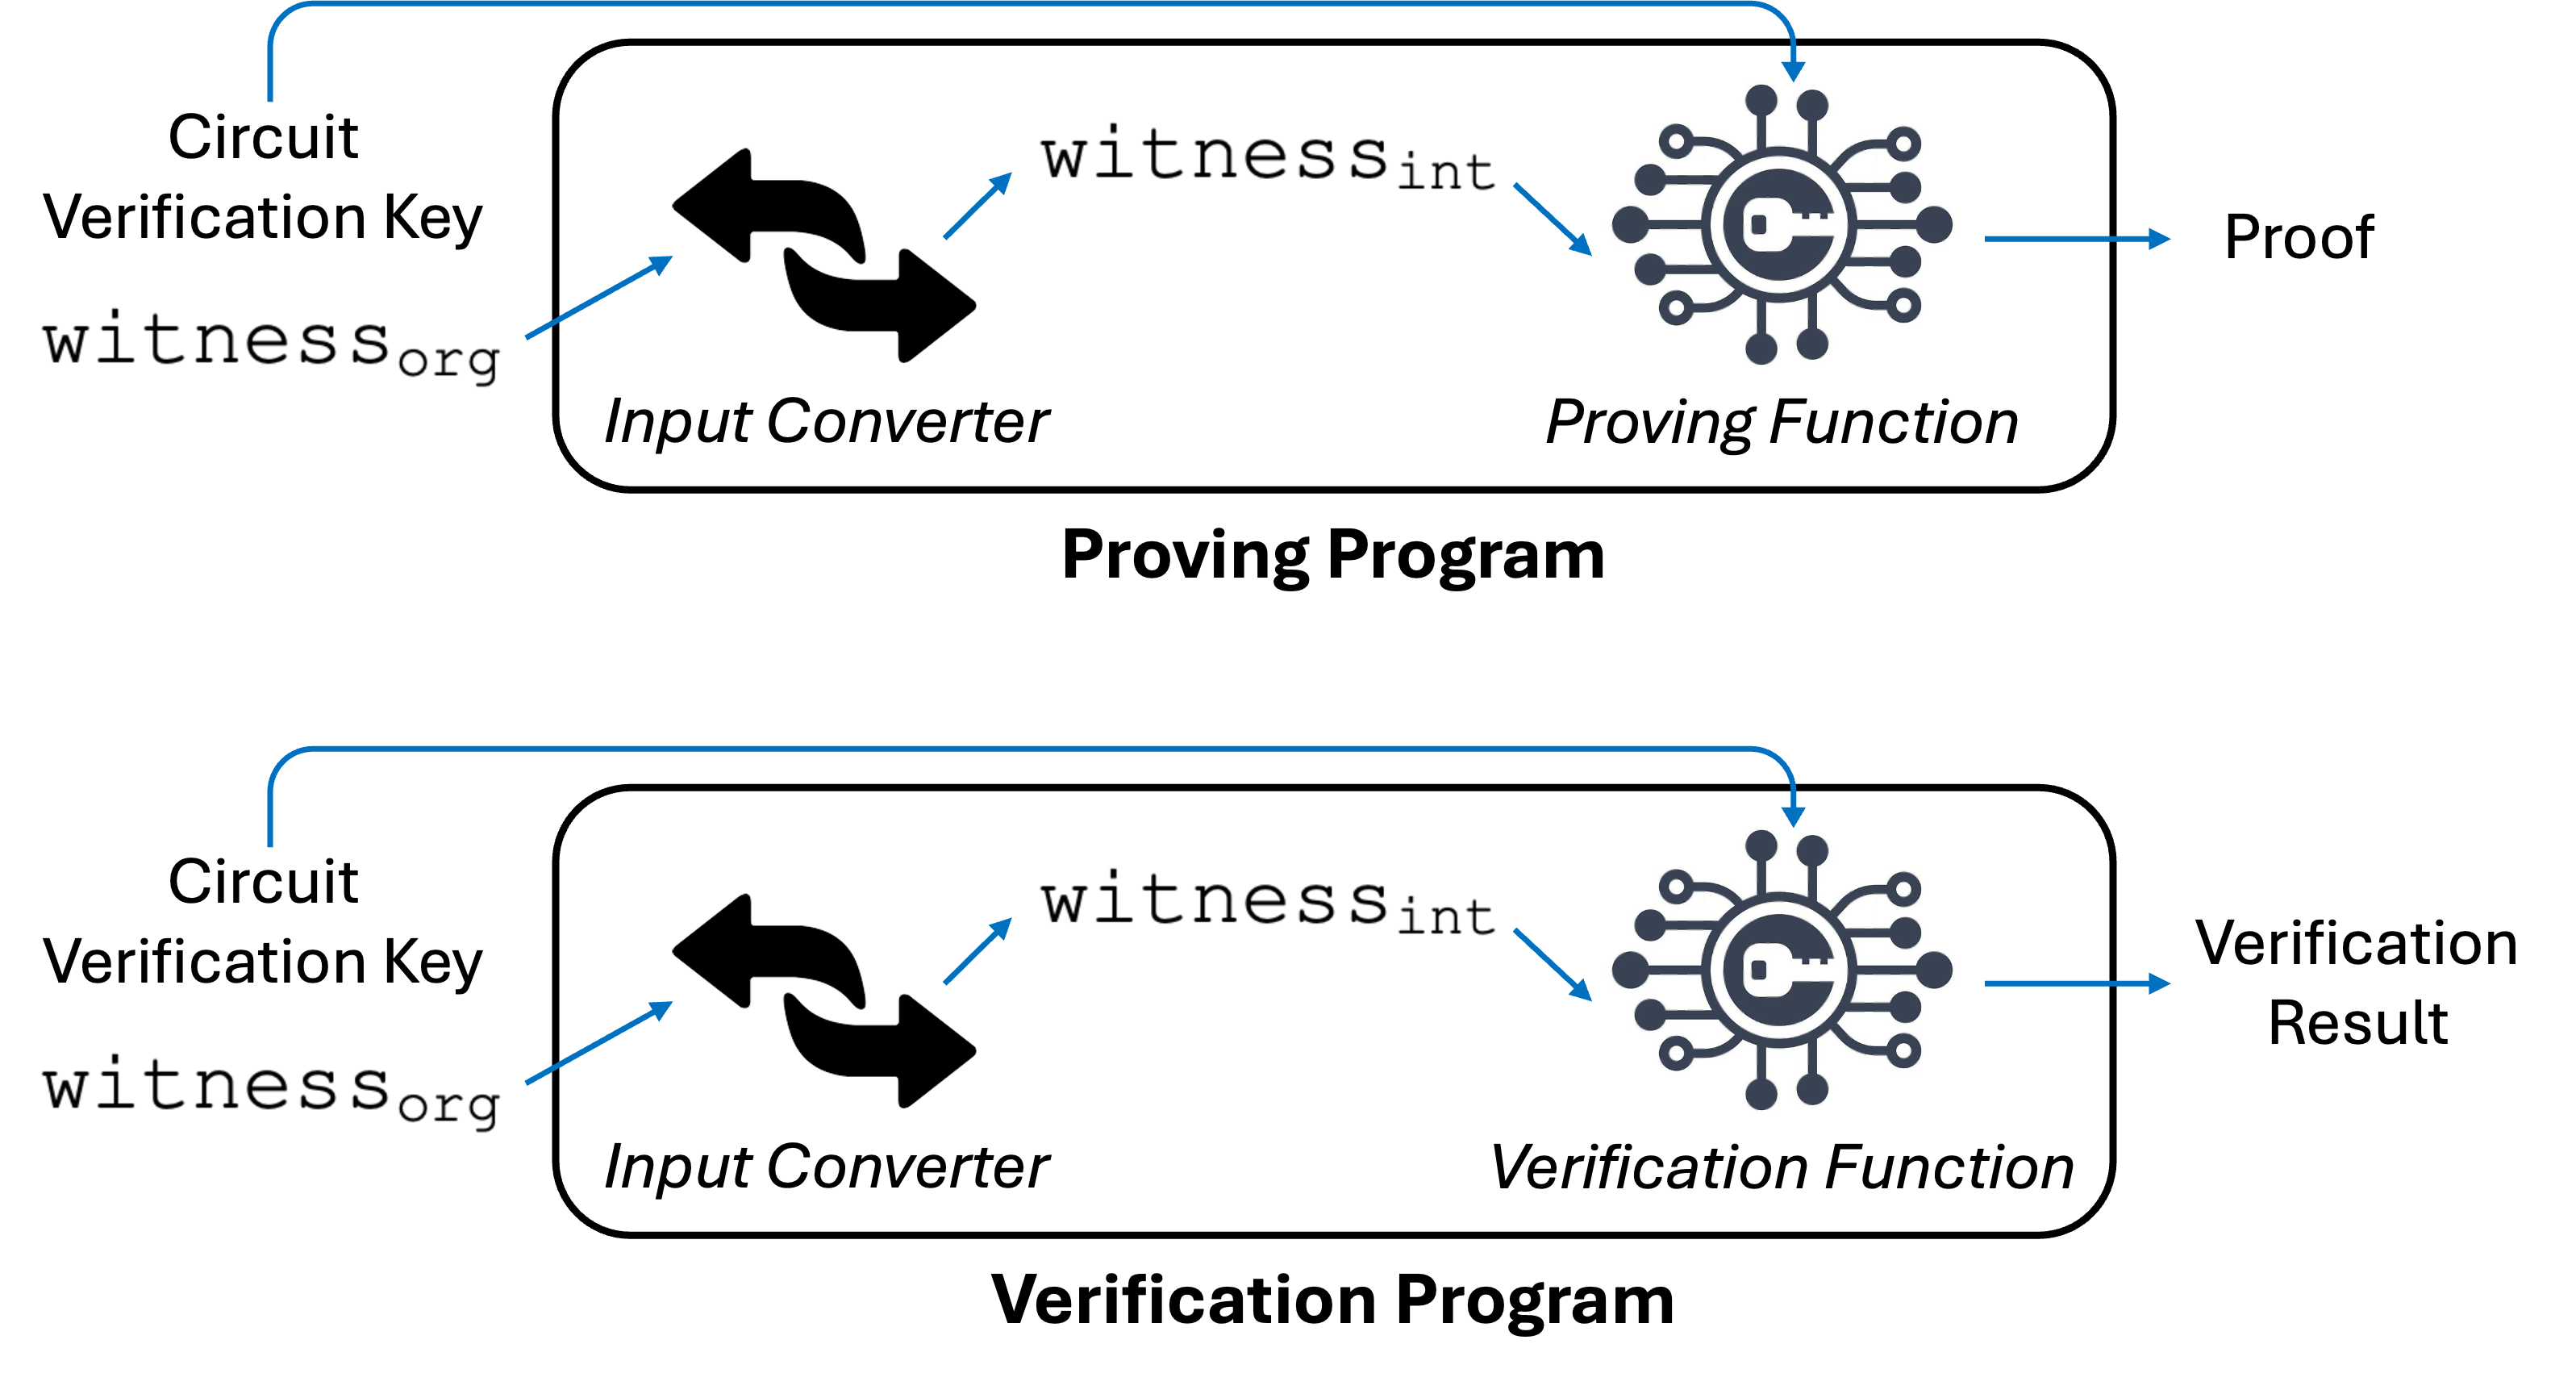
\includegraphics[width=0.5\textwidth,keepaspectratio]{./ch-greybox/figure/structure_zkp.png}
  \caption{Structure of a \zksnark program. }
  \label{fig:structure_zkp}
\end{figure}

A \zksnark application typically contains two complete programs: a prover-side program, denoted by \pprog, and a verifier-side program, denoted by \vprog. Each complete program contains both general program logic and a core cryptographic function. \autoref{fig:structure_zkp} illustrates this structure.

The prover-side program \pprog receives the original witness \witnessorg, a circuit representation such as a Rank-1 Constraint System (R1CS), and a proving key. The original witness contains both public and private values. Since the core proof-generation function \pfunc operates on the algebraic format required by the underlying proof system, \pprog first applies an \inputconvert step to transform \witnessorg into the internal witness representation \witnessint. This internal representation typically encodes values in forms suitable for proof computation, such as finite-field elements, ordered vectors, or other system-specific structures, rather than the original application-level format. For example, an application may provide a witness value as a decimal integer or a structured object, while the proof system requires that value to be represented as one or more finite-field elements in a fixed order. After this conversion, \pfunc uses \witnessint, the circuit, and the proving key to generate a proof.%, since the proof-generation algorithm operates over the field and group representations required by the underlying proof system rather than directly on application-level values.

The verifier-side program \vprog receives the proof, the public witness, and a verification key. The verifier does not receive the prover's private witness. However, the public witness still needs to be parsed and converted into the internal representation expected by the verification function \vfunc. Therefore, similar to \pprog, \vprog also contains an \inputconvert step for public witness. After conversion, \vfunc checks the proof with respect to the public witness and verification key, and outputs either accept or reject.

This structure creates several possible sources of \logicerror. An inconsistency may originate from the circuit, the prover-side \inputconvert, the proof-generation function, the verifier-side \inputconvert, or the verification function. Therefore, detecting that an error exists is not sufficient. A practical testing tool should also help locate which component is responsible for the error.

Depending on the specific proof system, a setup phase may also be required before \pprog and \vprog are executed. For example, many \zksnark protocols require a setup process to generate parameters such as proving key and verification key. These setup artifacts are treated as inputs to the corresponding prover and verifier programs.

In the remainder of this paper, we use the term \emph{software error} to refer to observable program failures, such as crashes, memory errors, assertion failures, or abnormal termination, and we use \logicerror{} to refer to cryptographically incorrect behavior that may not cause any runtime failure. We also distinguish between \programbranch, which handles general program functionality such as parsing, memory management, and input/output, and \cryptobranch, which performs cryptographic computation or directly influences cryptographic computation, such as proof generation, proof verification, finite-field arithmetic, elliptic-curve operations, constraint evaluation, and protocol-specific logic.

\subsection{Motivation for Grey-Box Fuzzing of \zksnark Programs}
\label{subsec:greybox-motivation_greybox}
General-purpose fuzzing tools are effective at detecting software errors in cryptographic programs. For example, fuzzers such as \afl can generate inputs that expose crashes, buffer overflows, null pointer dereferences, and other memory-safety issues. However, many serious errors in \zksnark implementations are \logicerror{}s rather than ordinary software errors. A \zksnark program may execute successfully but still produce an incorrect proof, accept an invalid proof, reject a valid proof, or enforce a statement different from the intended one. Since these errors may not cause crashes or abnormal termination, crash-oriented fuzzing alone cannot reliably detect them.

Differential fuzzing provides a more suitable foundation for detecting \logicerror because it checks whether the target implementation produces the expected cryptographic result rather than merely observing whether the program crashes. In principle, a fuzzer can compare the output of a target \zksnark program against the expected accept-or-reject result of the intended statement and report inconsistencies such as accepting an invalid witness or rejecting a valid one. This makes differential fuzzing a natural starting point for testing \zksnark correctness.

Among possible differential fuzzing designs, a grey-box approach is particularly suitable for real-world \zksnark applications. Unlike source code based approaches, grey-box fuzzing can be applied directly to deployed binary programs, which is important when source code is unavailable. At the same time, it can use internal information from the target \zksnark program to improve testing efficiency. In our setting, this is especially valuable because \zksnark applications follow structured cryptographic workflows that can benefit from protocol-aware guidance even in binary-only form.

The first major obstacle is input generation. General-purpose fuzzers mutate byte sequences without understanding the structure or meaning of cryptographic inputs. As a result, they often produce malformed witnesses, invalid field elements, incorrectly encoded group elements, or proof objects that are rejected before execution reaches the core cryptographic computation. Although such inputs may still be useful for testing parsers or input validation code, they are inefficient for finding logic errors in proof generation or verification. To reach deeper cryptographic computation, the fuzzer must generate inputs that preserve the expected format while still exploring valid, invalid, and boundary-case values.

The second obstacle is coverage guidance. General fuzzers usually reward any input that discovers a new execution path. In \zksnark software, however, many execution paths are unrelated to cryptographic correctness, such as file parsing, memory allocation, data-structure handling, and general input/output code \cite{wen2024practical, 0xparc_zk_bug_tracker}. Exploring these paths may increase overall coverage, but it does not necessarily improve the chance of detecting proof-related logic errors. A more effective strategy is to identify the branches that depend on cryptographic inputs and prioritize inputs that exercise those branches.

These challenges motivate the design of \greyboxfuzz. By combining differential fuzzing with structure-aware input generation and cryptographic-branch-focused coverage guidance, \greyboxfuzz improves the practicality and efficiency of testing binary-only \zksnark applications.


\subsection{Workflow}
\label{subsec:greybox-workflow}

\begin{figure*}[t]
  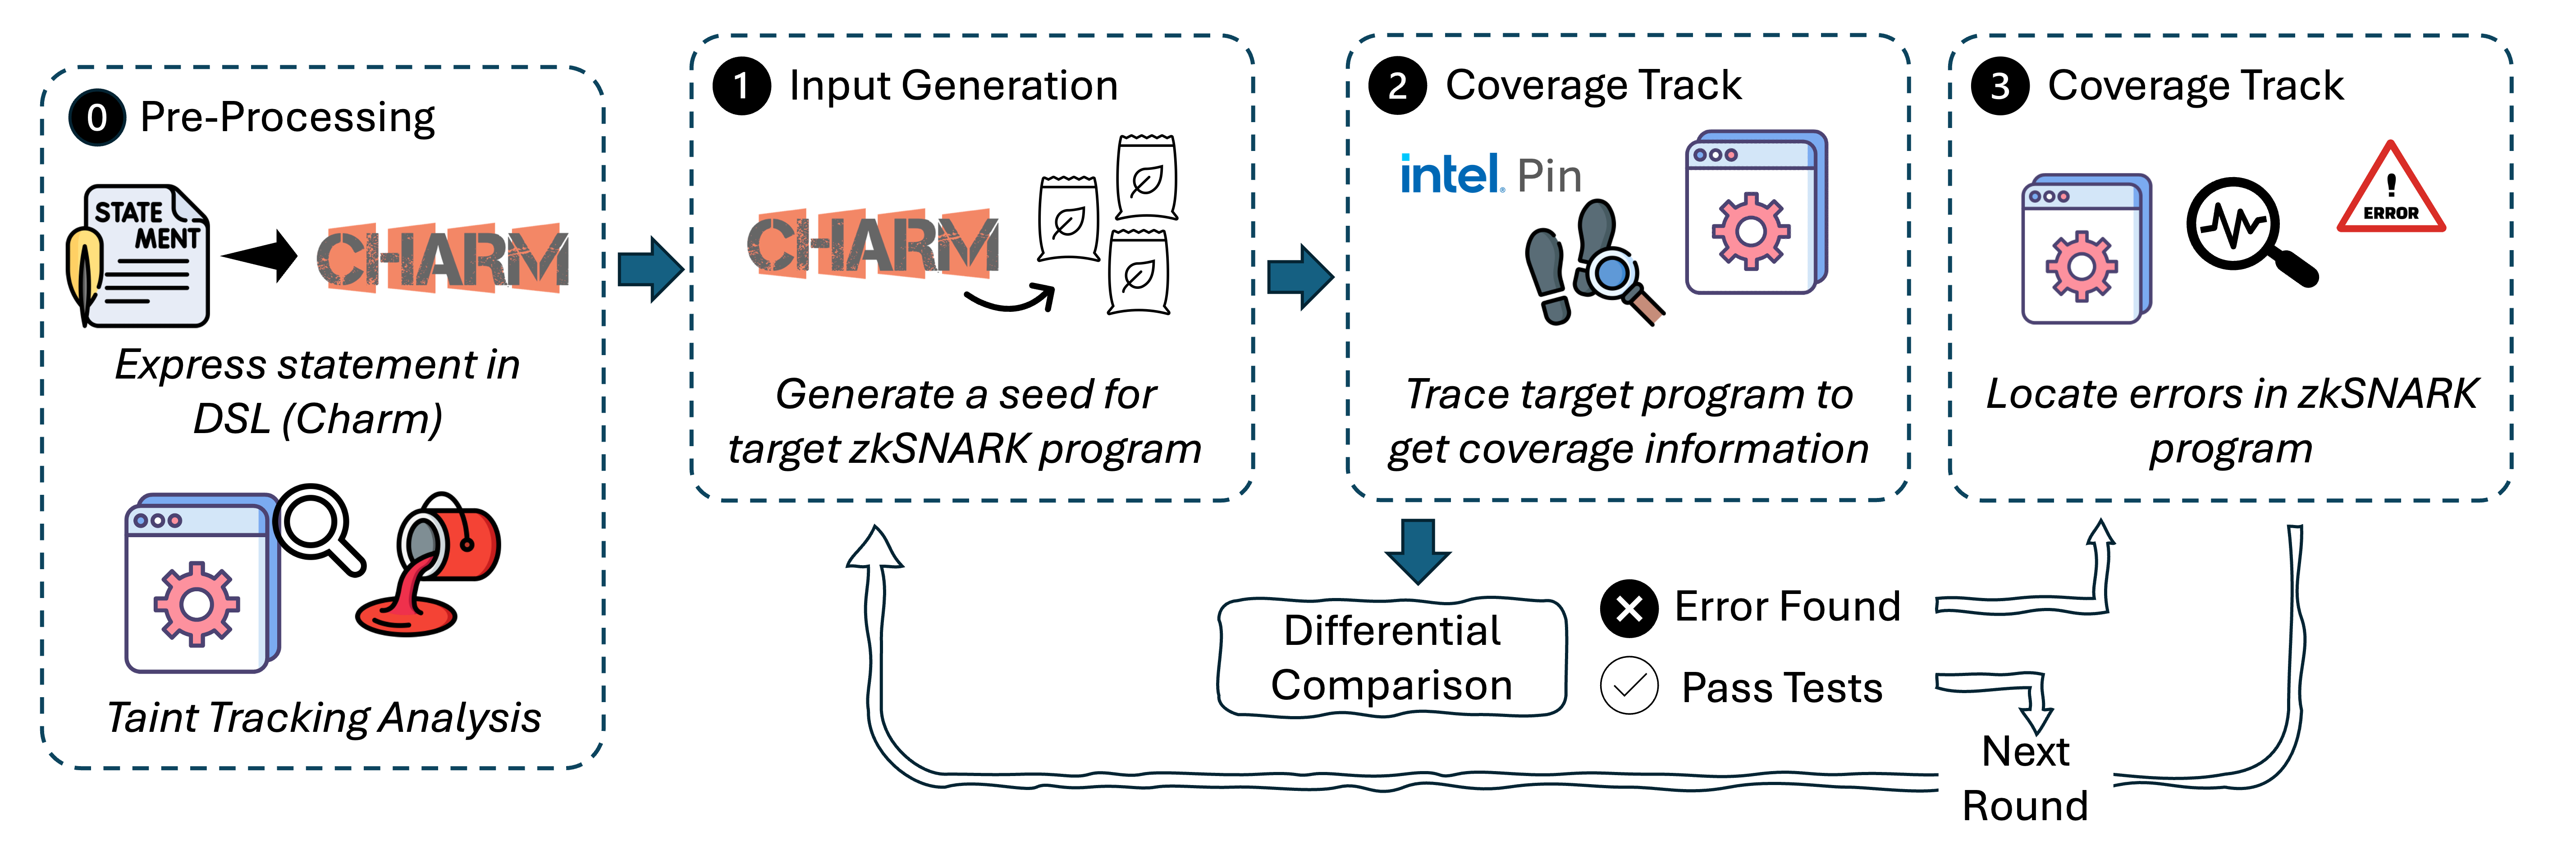
\includegraphics[width=\textwidth,keepaspectratio]{./ch-greybox/figure/overview.png}
  \caption{Overview of \greyboxfuzz.}
  \label{fig:overview}
\end{figure*}

\autoref{fig:overview} shows the workflow of \greyboxfuzz. To achieve the design goals and address the obstacles described in \autoref{subsec:greybox-motivation_greybox}, the workflow consists of five main components: differential test vector and ground truth for generating the expected result for a \zksnark program, preprocessing for investigating the target \zksnark program and obtaining additional information to improve fuzzing efficiency, input generation for producing suitable test inputs for effective fuzzing of \zksnark programs, coverage monitoring for tracking testing progress, and error localization as a new feature not provided by previous fuzzing tools.

\parhead{Differential ground truth}
For each generated seed, \greyboxfuzz executes the target \pprog and \vprog and compares the output with the expected result derived from the user-provided statement. In this process, the high-level cryptographic statement serves as the test vector and ground truth. Instead of requiring developers to implement a separate reference program for the entire \zksnark program, \greyboxfuzz evaluates the generated inputs against the statement to obtain the expected result and then compares that result with the output of the target binary program. If both results agree, the seed does not expose a \logicerror. If the target program accepts an input that should be rejected, rejects an input that should be accepted, or otherwise produces a result inconsistent with the statement, \greyboxfuzz reports a potential error.

\parhead{Preprocessing}
Before fuzzing begins, \greyboxfuzz performs a one-time analysis of the target binary programs. Since \greyboxfuzz targets binary-only \zksnark programs, it cannot rely on source-code instrumentation. Instead, it applies static taint tracking to identify \cryptobranch in the target binaries. These branches are the parts of the program that depend on \zksnark inputs, such as the witness, circuit, proving key, verification key, and proof. Identifying these branches allows \greyboxfuzz to distinguish security-relevant cryptographic computation from general program logic.

During preprocessing, \greyboxfuzz also identifies program locations needed by the error locator. These locations are used to separate the complete prover and verifier programs into smaller logical components, such as \inputconvert, proof generation, and proof verification. This enables \greyboxfuzz to provide more useful feedback when it detects an inconsistency and helps narrow the component most likely responsible for the error.

\parhead{Input generation}
After preprocessing, \greyboxfuzz generates and mutates input seeds for the target program. Unlike general-purpose fuzzers, \greyboxfuzz uses a structure-aware input formatter that understands the structure of the cryptographic statement. The user provides the intended statement in a domain-specific language, and \greyboxfuzz uses this statement to infer the expected input types and constraints. In our current implementation, we use Charm as the domain-specific language tool. The formatter extracts variable information from the statement written with Charm and uses it to guide both seed generation and mutation. It distinguishes among input structure, mathematical validity, and statement-level value validity. This design allows \greyboxfuzz to produce seeds that preserve the legal format expected by the target program while still exploring invalid, boundary-case, and security-relevant values.

\parhead{Coverage monitoring}
During execution, \greyboxfuzz records which binary instructions are visited by each seed. Because \greyboxfuzz focuses on \logicerror, it does not treat all new execution paths equally. Instead, it prioritizes seeds that visit new \cryptobranch. To support this strategy, \greyboxfuzz combines static taint tracking with dynamic tracing. Static taint tracking identifies instructions that belong to the cryptographic related branches, while dynamic tracing records whether generated seeds reach those cryptographic-related branches. Inputs that explore new \cryptobranch are prioritized, whereas inputs that only expand general programming coverage receive less attention. This prevents the fuzzer from spending excessive time exploring general parsing, input/output, or memory-management code when those paths do not affect the cryptographic result.

\parhead{Error localization}
When \greyboxfuzz detects an inconsistency, it invokes the error locator. A \zksnark program may fail because of an incorrect implementation in circuit, \inputconvert, proof-generation function \pfunc, or verification function \vfunc. The error locator therefore analyzes multiple intermediate components, including the circuit, converted witness values, proof-generation behavior, and verification behavior, to narrow the source of the error. Instead of only reporting that the target program failed, \greyboxfuzz attempts to identify whether the error is caused by the circuit, the prover-side \inputconvert, \pfunc, the verifier-side \inputconvert, or \vfunc. This feedback helps developers diagnose and fix \logicerror in binary-only \zksnark implementations.

\subsection{Users and Use Cases}
\label{subsec:greybox-users_use_cases}

\greyboxfuzz is designed for users who need to evaluate the correctness and security of a specific \zksnark application but may not have the ability to audit the entire implementation manually. This includes both prover-side and verifier-side users.

From the prover's perspective, the main concern is whether the program correctly proves the intended statement using the provided witness. A prover-side error may cause a valid witness to be converted incorrectly, a valid proof to fail, or the proof-generation process to enforce a statement different from the intended one.

From the verifier's perspective, the main concern is whether an invalid proof can be accepted. If a prover can generate a proof using values that do not satisfy the intended statement, then the verifier should not trust the proof in that setting. Such a result may indicate an error in the circuit, witness conversion, proof generation, verification, or the surrounding program logic.

To use \greyboxfuzz, the user provides the prover binary program, the verifier program, and the \zksnark statement written with Charm. \greyboxfuzz then generates test inputs, checks the target program against the statement, monitors cryptographic coverage, and reports both detected inconsistencies and their likely locations. This allows users to evaluate a specific proof application without requiring source-code access or a complete manual audit of the underlying \zksnark library.



\section{Differential Fuzzing}
\label{sec:greybox-differential}

The goal of differential fuzzing in \greyboxfuzz is to determine whether the target \zksnark program returns the correct verification result for a specific witness. Traditional differential fuzzing usually compares multiple implementations of the same specification. This strategy is difficult to apply directly to \zksnark programs because each application may encode a different statement, and building an independent \zksnark implementation for every statement is expensive and error-prone. Instead of requiring a second \zksnark implementation as the reference, \greyboxfuzz uses the intended statement itself as the test vector.

For each generated seed, \greyboxfuzz first evaluates whether the seed satisfies the statement that the target \zksnark program is intended to prove, and uses this evaluation to derive the expected verification result, namely accept or reject. The target prover and verifier are then executed on the same seed, and \greyboxfuzz compares the verifier's final decision against this expected result. Thus, the differential check is performed on the verification outcome only, rather than on the generated proof object itself. This distinction is important because two correct prover executions on the same input may still produce different proofs due to prover randomness, even though both proofs should lead to the same verification result. If the expected result and the verifier's decision agree, the seed does not expose an inconsistency. If they disagree, \greyboxfuzz reports a potential \logicerror. For example, if the statement is knowledge of a secret exponent $x$ such that $h = g^x$, where $g$ and $h$ are public values and $x$ is private, \greyboxfuzz does not require a second \zksnark prover and verifier as the reference. Instead, it only requires an independent program that checks whether the relation $h = g^x$ holds for the generated input and returns the corresponding accept-or-reject ground truth, without comparing the actual proofs themselves.

This design changes the role of test vectors in \greyboxfuzz. Rather than using fixed \zksnark test vectors or manually constructing a separate reference implementation, \greyboxfuzz generates new seeds during fuzzing and evaluates each seed against the statement. This is important because \logicerror often appears only for specific boundary cases, malformed but parseable values, or witness that violate the intended statement while still satisfying the program's expected format. By computing the expected result for each generated seed, \greyboxfuzz can detect cases where the target program accepts an invalid witness, rejects a valid witness, or produces a verification result inconsistent with the intended statement.

To reduce the burden of writing the \zksnark statement, \greyboxfuzz uses Charm \cite{akinyele2013charm}. Charm is a framework for prototyping cryptographic systems and provides high-level abstractions for common cryptographic objects and operations, including group elements, finite-field values, exponentiation, hashing, and pairing-based operations. Instead of asking the user to manually implement low-level cryptographic computations, \greyboxfuzz allows user to express the intended statement in Charm. The Charm program serves as the test vector and ground truth that computes the expected verification result for each generated seed.

For example, the statement $h = g^x$ can be expressed at a high level by declaring $g$ and $h$ as public group elements and $x$ as a private exponent. Conceptually, the statement has the following form with Charm:

\begin{ZZlisting}[H]
\centering
\begin{adjustbox}{max width=\textwidth}
\begin{CenteredBox}
\begin{minipage}{0.96\textwidth}
\begin{lstlisting}[style=pythonstyle]
from charm.toolbox.eccurve import prime192v1
from charm.toolbox.ecgroup import ECGroup

group = ECGroup(prime192v1)
g = group.random()
x = group.random()
h = g ** x

def oracle(g, h, x):
    return h == g ** x

\end{lstlisting}
\end{minipage}
\end{CenteredBox}
\end{adjustbox}
\caption{An example of Charm implementation}
\label{list:charm}
\end{ZZlisting}


The actual Charm implementation handles the underlying cryptographic representation of the variables, so the user does not need to manually implement elliptic-curve arithmetic or finite-field operations. This makes the statement easier to write and less likely to introduce unrelated implementation mistakes. The user only needs to describe the mathematical relationship that the proof is intended to enforce.

After the statement is defined, \greyboxfuzz uses it during fuzzing as follows. First, the input formatter generates a seed according to the expected structure of the statement. Second, the seed is evaluated by Charm to obtain the expected accept or reject result. Third, the same seed is passed to the target \pprog and \vprog to obtain the actual verification result. Finally, \greyboxfuzz compares the expected result with the actual result. A mismatch indicates that the target \zksnark program may not correctly implement the intended statement.

This statement-level test vector provides two advantages. First, it avoids the need to construct a separate \zksnark implementation for every target program. Second, it allows \greyboxfuzz to test the semantic correctness of the target program rather than only its ability to execute without crashing. As a result, \greyboxfuzz can detect \logicerror that would be missed by crash-oriented fuzzing, including missing constraints, incorrect witness conversion, invalid boundary handling, and incorrect proof or verification behavior.



\section{Input Formatter}
\label{sec:input_formatter}

The effectiveness of fuzzing depends heavily on the quality of the generated inputs. For programs with simple input formats, random mutation may be sufficient to reach meaningful program states. However, \zksnark programs require highly structured inputs, including public inputs, private witnesses, finite-field elements, elliptic-curve points, keys, proofs, and circuit-related data. If these inputs do not satisfy the expected format, the program often rejects them during parsing or early validation. As a result, a general-purpose fuzzer may spend most of its time generating inputs that never reach the cryptographic computation where \logicerror may occur.

To address this problem, \greyboxfuzz uses an input formatter that generates and mutates seeds according to the structure of the target statement. The input formatter does not attempt to prove that every generated seed is semantically valid. Instead, its goal is to preserve the legal input format required by the target \zksnark program while still allowing the fuzzer to explore valid values, invalid values, and boundary cases. This design allows \greyboxfuzz to avoid wasting most fuzzing iterations on malformed inputs and increases the probability that generated seeds reach \pfunc and \vfunc.

The input formatter is built on the statement-level oracle described in \autoref{sec:differential}. Since the user expresses the intended statement in Charm, \greyboxfuzz can use the same statement description to infer the structure of the required inputs. For example, a Charm statement may declare variables as integers, finite-field elements, group elements, or other cryptographic objects. \greyboxfuzz extracts this information and uses it to guide seed generation and mutation. This provides a lightweight structure-aware fuzzing layer without requiring source-code access to the target \zksnark binary.

\subsection{Seed Scheduling}

Not all generated seeds are equally useful for detecting \logicerror. Some inputs are rejected before they reach the cryptographic computation, while others exercise proof generation and verification but represent invalid statement-level values. To prioritize more useful seeds, \greyboxfuzz classifies generated inputs using three properties: \textbf{structure}, \textbf{mathematical validity}, and \textbf{statement-level value}. \autoref{tab:seed_scheduling} shows the scheduling priority used by \greyboxfuzz.

\textbf{Structure} describes whether the seed has the expected syntactic format. For example, if the target program expects a witness containing integer values, then a string or floating-point value has an invalid structure. If the target program expects an elliptic-curve point, then the seed must contain the components required to represent that point. Inputs with invalid structure are usually rejected during parsing or cause ordinary software failures. They are therefore less useful for detecting \logicerror, which usually occurs after the program reaches cryptographic computation.

\textbf{Mathematical validity} describes whether the seed satisfies the algebraic constraints required by the input type. For example, a finite-field element must lie within the field range, and an elliptic-curve point must represent a valid point on the selected curve. A seed may have the correct structure but still violate these mathematical requirements. Such inputs are useful for testing whether the target program correctly validates cryptographic objects and rejects invalid mathematical values.

\textbf{Statement-level value} describes whether the seed satisfies the intended statement. For example, in a statement that proves knowledge of an age within an allowed range, the input may be a correctly formatted integer and may satisfy the mathematical type constraints, but still be invalid for the application if the value is outside the intended range. These inputs are important because many \logicerror arise when the program accepts values that have a legal format but do not satisfy the intended statement.

\begin{table}[t]
\centering
\begin{tabular}{c|c|c|c}
\hline
Priority & Structure & Mathematical Validity & Statement-Level Value \\ \hline\hline
1 & Valid & Valid & Valid \\ \hline
2 & Valid & Valid & Invalid \\ \hline
3 & Valid & Invalid & Invalid \\ \hline
4 & Invalid & Invalid & Invalid \\ \hline
\end{tabular}
\caption{Seed scheduling priority used by the input formatter.}
\label{tab:seed_scheduling}
\end{table}

This scheduling policy gives the highest priority to seeds that can reach the cryptographic computation and exercise the intended statement. It also preserves lower-priority invalid seeds because they may still expose input-validation bugs or software errors. However, \greyboxfuzz gives less fuzzing effort to structurally invalid seeds because they are unlikely to reveal \logicerror in proof generation or verification.

\subsection{Extracting Seed Structure}

The input formatter obtains seed structure from the Charm statement provided by the user. Charm represents cryptographic statements using high-level objects and operations, such as integers, finite-field elements, group elements, exponentiation, hashing, and pairing-related operations. \greyboxfuzz parses the Charm statement to identify the variables used by the statement, their roles as public or private inputs, and their expected types.

For built-in types, such as integers or byte strings, the formatter can directly generate values of the same type. For cryptographic types, the formatter records the internal structure required to serialize and mutate the value. For example, a finite-field element is generated within the modulus of the selected field. A group element is generated according to the representation expected by the group. If the target input is represented by multiple components, the formatter mutates each component while preserving the overall structure of the object.

This process allows \greyboxfuzz to generate inputs that match the type expectations of both the Charm oracle and the target \zksnark program. For example, consider a statement of the form \(h = g^x\), where \(g\) and \(h\) are public group elements and \(x\) is a private exponent. From this statement, \greyboxfuzz learns that \(g\) and \(h\) should be generated as group elements and that \(x\) should be generated as a scalar value in the appropriate field. The formatter can then generate seeds that preserve this structure while varying the actual values used for testing.

The input formatter only infers structural and mathematical constraints that are visible from the statement and its variable types. It does not automatically infer all application-level semantics. For example, if a variable represents a year or an age, Charm may only expose it as an integer. The formatter therefore knows how to generate an integer, but it may not know the intended application range unless the statement explicitly encodes that range. This distinction is important because \greyboxfuzz intentionally generates both valid and invalid statement-level values. Inputs that are structurally legal but semantically invalid are often the most useful for detecting \logicerror.

\subsection{Seed Generation and Mutation}

After extracting the seed structure, \greyboxfuzz generates inputs using two complementary strategies: grammar-based generation and structure-preserving mutation.

\parhead{Grammar-based generation}
The formatter first generates seeds from the extracted input structure. Each generated seed follows the expected format of the target statement. For example, if an input is a finite-field element, the formatter generates a value in the corresponding field representation. If an input is a group element, the formatter generates a value using the representation expected by the selected group. This strategy increases the probability that generated seeds pass parsing and early validation, allowing the execution to reach proof generation and verification.

\parhead{Structure-preserving mutation}
The formatter also mutates previously generated seeds while preserving their high-level structure. Instead of applying arbitrary byte-level mutations, \greyboxfuzz mutates individual fields according to their types. For example, it may replace a scalar with another scalar, change a field element to a boundary value, or modify one component of a structured cryptographic object while keeping the object in a legal encoding. This allows \greyboxfuzz to explore nearby inputs without destroying the format needed by the target program.

\greyboxfuzz also generates negative test cases. These inputs intentionally violate mathematical or statement-level requirements while preserving the legal format. For example, a seed may use a value outside the intended application range, or it may fail to satisfy the statement while still being correctly encoded. Such inputs are important because a secure implementation should reject them. If the target program accepts one of these inputs, \greyboxfuzz reports a potential \logicerror.

\begin{table}[t]
\centering
\begin{tabular}{c|c|c}
\hline
Generation Strategy & Format & Expected Statement Result \\ \hline\hline
Grammar-based & Legal & Accept \\ \hline
Grammar-based & Legal & Reject \\ \hline
Grammar-based & Illegal & Reject \\ \hline
Mutation-based & Legal & Accept \\ \hline
Mutation-based & Legal & Reject \\ \hline
Mutation-based & Illegal & Reject \\ \hline
\end{tabular}
\caption{Input generation strategies used by \greyboxfuzz.}
\label{tab:input_formatter}
\end{table}

\autoref{tab:input_formatter} summarizes the input generation strategies used by \greyboxfuzz. Legal-format inputs are the primary focus because they are more likely to reach the cryptographic computation. Among them, both accepting and rejecting cases are necessary: accepting cases test whether valid witnesses are handled correctly, while rejecting cases test whether invalid witnesses are incorrectly accepted. Illegal-format inputs are assigned lower priority but are still useful for detecting ordinary software errors and input-validation failures.

By combining statement derived structure, priority based scheduling, and structure preserving mutation, the input formatter improves the efficiency of fuzzing \zksnark programs. It reduces the number of seeds rejected before cryptographic execution and increases the number of test cases that exercise proof generation, proof verification, and statement-level correctness.


%%%%%%%%%%%%%%%%%%%%%%%%%%%%%%%%%

\section{Coverage Monitor}
\label{sec:coverage_monitor}

The coverage monitor guides \greyboxfuzz toward the parts of a \zksnark binary that are most relevant to detecting \logicerror. General-purpose fuzzers usually treat all newly discovered execution paths as useful. This strategy is effective for finding crashes and memory errors, but it is inefficient for \zksnark programs because many execution paths only involve parsing, file handling, memory allocation, or other general program logic. These paths may improve overall code coverage without improving the chance of detecting cryptographic correctness errors.

\greyboxfuzz therefore uses a cryptographic-branch-focused coverage strategy. Instead of prioritizing every new path, \greyboxfuzz first identifies the instructions that are related to cryptographic computation and then gives higher priority to seeds that exercise new instructions in those regions. This allows the fuzzer to spend more time testing proof generation, proof verification, witness conversion, finite-field arithmetic, elliptic-curve operations, and other computation that can affect the final verification result.

The coverage monitor has two stages. First, before fuzzing begins, \greyboxfuzz performs static taint tracking on the target binaries to classify instructions as either \cryptobranch or \programbranch. Second, during fuzzing, \greyboxfuzz dynamically traces executed instructions and records whether each seed visits new \cryptobranch. The resulting feedback is used to guide seed scheduling and to determine whether the cryptographic portion of the target program has been sufficiently explored.

\subsection{\zksnark Code Branches}
\label{subsec:zkp_code_branch}

\greyboxfuzz separates the target binary into two categories of code: \cryptobranch and \programbranch. A \cryptobranch is an instruction or code region that performs cryptographic computation or directly influences cryptographic computation. This includes operations related to witness conversion, constraint evaluation, proof generation, proof verification, finite-field arithmetic, elliptic-curve operations, and pairing-based computation. A \programbranch is an instruction or code region that handles general program functionality, such as input/output, parsing, memory management, data-structure operations, or language-runtime behavior.

This distinction is important because \greyboxfuzz targets \logicerror rather than ordinary software errors. A software error, such as a crash or invalid memory access, may occur in either \cryptobranch or \programbranch. In contrast, a \logicerror is caused by incorrect cryptographic behavior, such as accepting an invalid proof, rejecting a valid proof, incorrectly converting a witness, or enforcing a statement different from the intended one. These errors are most likely to appear in code that participates in cryptographic computation or directly affects the values used by that computation.

Therefore, \greyboxfuzz does not require complete coverage of the entire binary before providing useful feedback. Instead, it focuses on coverage of \cryptobranch. If the fuzzer has already generated seeds that exercise the identified \cryptobranch, continuing to explore unrelated \programbranch may provide limited additional benefit for detecting \logicerror. This targeted coverage strategy improves fuzzing efficiency while preserving the ability to test the security-relevant parts of the program.

\subsection{Branch Identification}
\label{subsec:branch_identify}

Before fuzzing begins, \greyboxfuzz identifies \cryptobranch in the target \pprog and \vprog. In a \zksnark program, the prover computes proof elements from the witness, circuit, proving key, and protocol-specific randomness. The verifier checks the proof using the public input, verification key, and proof object. These computations depend on cryptographic inputs and determine whether the final verification result is correct. Therefore, \greyboxfuzz uses taint tracking to identify instructions whose values are derived from, or controlled by, these cryptographic inputs.

\greyboxfuzz uses static taint tracking for this identification step. Static analysis is useful because it can inspect the binary without requiring a particular execution path to be triggered by a seed. Dynamic taint tracking only observes the paths executed by the current inputs, so it may miss \cryptobranch that are not reached during early fuzzing. In contrast, static taint tracking allows \greyboxfuzz to build an initial map of potentially relevant cryptographic instructions before the fuzzing loop begins.

For \pprog, \greyboxfuzz initializes the circuit, witness, and proving key as taint sources. For \vprog, \greyboxfuzz initializes the public input, proof, and verification key as taint sources. Instructions that compute values from these sources, move tainted values through registers or memory, or execute under conditions affected by these sources are marked as \cryptobranch. Other instructions are treated as \programbranch unless later analysis shows that they influence cryptographic computation.

\subsection{Control-Dependency-Aware Taint Tracking}
\label{subsec:control_dependency_taint}

A direct data-dependency taint tracker is not sufficient for identifying all \cryptobranch. Traditional taint tracking usually propagates taint when a value is directly computed from a tainted value. For example, if \(x\) is tainted and \(y = x + 1\), then \(y\) is also tainted. However, this approach misses implicit dependencies introduced by control flow. If \(x\) determines which branch is executed and \(y\) is assigned inside that branch, then \(y\) depends on \(x\) even if the assignment does not directly use \(x\).

\autoref{list:taintdiff} illustrates this limitation. In Option 1, \(y\) is directly computed from the tainted variable \(x\), so a traditional taint tracker marks \(y\) as tainted. In Option 2, the value of \(y\) is selected by a branch condition involving \(x\). Although neither assignment directly uses \(x\), the final value of \(y\) still depends on \(x\). A direct data-dependency tracker may fail to mark \(y\) as tainted, causing \greyboxfuzz to miss instructions that are logically influenced by cryptographic inputs.

\begin{ZZlisting}[H]
\centering
\begin{adjustbox}{max width=\textwidth}
\begin{CenteredBox}
\begin{minipage}{0.96\textwidth}

\begin{minipage}[t]{0.47\textwidth}
Option 1

\vspace{0.3em}
\hrule
\vspace{0.5em}

\begin{lstlisting}[style=cstyle]
int x = strtol(argv[1], NULL, 10);
if (x > VALUE)
    int y = x + 1;
else
    int y = x - 1;
\end{lstlisting}
\end{minipage}
\hfill
\begin{minipage}[t]{0.47\textwidth}
Option 2

\vspace{0.3em}
\hrule
\vspace{0.5em}

\begin{lstlisting}[style=cstyle]
int x = strtol(argv[1], NULL, 10);
if (x > VALUE)
    int y = 11;
else
    int y = 9;
\end{lstlisting}
\end{minipage}

\end{minipage}
\end{CenteredBox}
\end{adjustbox}
\caption{Direct data-dependency taint tracking can miss values that depend on tainted inputs through control flow.}
\label{list:taintdiff}
\end{ZZlisting}


% \begin{table}[t]
% \centering
% \begin{tabular}{|p{3.9cm}|p{3.9cm}|}
% \hline
% Option 1 & Option 2 \\ \hline
% \begin{lstlisting}[style=C]
% int (*@\textcolor{red}{x}@*) = strtol(argv[1], NULL, 10);
% if ((*@\textcolor{red}{x}@*) > VALUE)
%     int (*@\textcolor{orange}{y}@*) = (*@\textcolor{red}{x}@*) + 1;
% else
%     int (*@\textcolor{orange}{y}@*) = (*@\textcolor{red}{x}@*) - 1;
% \end{lstlisting}
% &
% \begin{lstlisting}[style=C]
% int (*@\textcolor{red}{x}@*) = strtol(argv[1], NULL, 10);
% if ((*@\textcolor{red}{x}@*) > VALUE)
%     int (*@\textcolor{orange}{y}@*) = 11;
% else
%     int (*@\textcolor{orange}{y}@*) = 9;
% \end{lstlisting}
% \\ \hline
% \end{tabular}
% \caption{Direct data-dependency taint tracking can miss values that depend on tainted inputs through control flow.}
% \label{tab:taintdiff}
% \end{table}

To address this limitation, \greyboxfuzz uses a control-dependency-aware taint tracking strategy. In addition to propagating taint through explicit data movement and arithmetic operations, \greyboxfuzz also propagates taint to values assigned inside a conditional region controlled by a tainted condition. This is important for cryptographic programs because input-dependent branches may select different constants, table entries, validation outcomes, or protocol states. Even when a value is not directly computed from a tainted input, it may still influence the cryptographic result.

The static taint tracker operates on assembly instructions and maintains two taint states: tainted memory locations and tainted registers. It applies the following rules:

\begin{itemize}[leftmargin=*]
    \setlength{\itemsep}{0pt}
    \setlength{\parskip}{0pt}

    \item A register becomes tainted when a tainted memory value or another tainted register is moved into it.

    \item A register becomes untainted when it is overwritten by a value that is not derived from tainted data.

    \item A memory location becomes tainted when a value derived from tainted data is written to it.

    \item An instruction is marked as \cryptobranch when it reads, writes, computes, or propagates tainted data.

    \item If a branch condition depends on tainted data, values assigned inside the corresponding control-dependent region are treated as tainted.

    \item A function return value is treated as tainted if the function receives tainted input or accesses tainted memory during its computation.
\end{itemize}

During this process, \greyboxfuzz records the offset of each instruction marked as \cryptobranch. The tracker records offsets rather than runtime addresses because static analysis does not execute the program and therefore does not observe the actual loaded addresses. Using offsets also avoids inconsistencies caused by Address Space Layout Randomization (ASLR), since the same instruction may be loaded at different runtime addresses across executions.


\begin{ZZlisting}[H]
\centering
\begin{adjustbox}{max width=\textwidth}
\begin{CenteredBox}
\begin{minipage}{0.96\textwidth}
\begin{lstlisting}[style=asmstyle]
0x0000113f <+22>:    mov    -0xc(%rbp),%edx
0x00001142 <+25>:    mov    -0x8(%rbp),%eax
0x00001145 <+28>:    add    %edx,%eax
0x00001147 <+30>:    mov    %eax,-0x4(%rbp)
0x0000114a <+33>:    mov    $0x3,%eax
\end{lstlisting}
\end{minipage}
\end{CenteredBox}
\end{adjustbox}
\caption{Example of instruction-level taint propagation. If \texttt{-0xc(\%rbp)} is tainted, then \texttt{\%edx} becomes tainted and the addition at offset \texttt{0x00001145} is marked as \cryptobranch.}
\label{list:asm}
\end{ZZlisting}


\autoref{list:asm} shows a simple example. If the memory location \texttt{-0xc(\%rbp)} is tainted, the first instruction moves the tainted value into \texttt{\%edx}. The instruction at offset \texttt{0x00001145} then performs an addition using \texttt{\%edx}. Because this computation uses tainted data, \greyboxfuzz marks this instruction as \cryptobranch. The resulting instruction offset is later used by the dynamic coverage monitor to determine whether a fuzzing seed exercised this cryptographic computation.

Although the taint tracker is designed for \zksnark programs in this paper, the same strategy can be applied more broadly to other cryptographic protocols whose security-relevant computation depends on identifiable protocol inputs. For example, proof systems such as Bulletproofs or other zero-knowledge protocols also compute protocol outputs from witnesses, public statements, commitments, and public parameters. As long as these inputs can be identified as taint sources, the same taint tracking strategy can be used to distinguish cryptographic computation from general program logic.

\subsection{Branch Tracking}
\label{subsec:branch_tracking}

After \greyboxfuzz identifies \cryptobranch statically, it monitors branch visits dynamically during fuzzing. For each generated seed, \greyboxfuzz executes the target binary and records which instructions are executed. The goal is to determine whether the seed reaches new \cryptobranch, not merely whether it increases total program coverage.

\greyboxfuzz uses Intel PIN to instrument the target binary and trace execution at the basic-block level. For each executed basic block, \greyboxfuzz iterates over its instructions and computes the offset of each instruction relative to the loaded binary base address. This offset representation matches the offsets produced by static taint tracking, allowing \greyboxfuzz to compare runtime execution traces with the statically identified \cryptobranch set.



\begin{ZZlisting}[H]
\centering
\begin{adjustbox}{max width=\textwidth}
\begin{CenteredBox}
\begin{minipage}{0.96\textwidth}
\begin{lstlisting}[style=asmstyle]
2117a: mov rax, qword ptr [rip+0x199e7]
21181: test rax, rax
21184: jz 0x70f88305918a
21186: add qword ptr [rax+0x8], r12
2118a: mov rax, qword ptr [rip+0x19a57]
21191: test rax, rax
21194: jz 0x70f88305919a
21196: add qword ptr [rax+0x8], r12
2119a: mov rax, qword ptr [rip+0x19b1f]
\end{lstlisting}
\end{minipage}
\end{CenteredBox}
\end{adjustbox}
\caption{Example of runtime instruction offsets recorded by the dynamic branch tracker.}
\label{list:tracing}
\end{ZZlisting}



\autoref{list:tracing} shows an example of the tracing output. Each line contains the instruction offset and the corresponding disassembled instruction observed during execution. When a recorded offset matches an offset in the statically identified \cryptobranch set, \greyboxfuzz marks that \cryptobranch as visited for the current seed.

This information is used as fuzzing feedback. If a seed visits a previously unseen \cryptobranch, \greyboxfuzz treats it as valuable and prioritizes it for future mutation. If a seed only explores new \programbranch, \greyboxfuzz gives it lower priority because that path is less likely to expose \logicerror. This differs from general instrumentation-guided fuzzing, which typically rewards any new execution path. By focusing on cryptographic coverage, \greyboxfuzz improves the efficiency of fuzzing while still preserving the ability to detect ordinary software errors when malformed inputs cause crashes.

The branch tracking result also provides a stopping criterion. Instead of requiring complete coverage of the entire binary, \greyboxfuzz can report the coverage achieved over the identified \cryptobranch. This allows developers to determine whether the security-relevant portion of the target program has been sufficiently tested.
\section{Error Locator}
\label{sec:error_locator}

Differential fuzzing can determine whether a target \zksnark program produces a result that is inconsistent with the statement-level oracle. However, this result alone does not tell developers where the error occurs. A mismatch may be caused by an incorrect circuit, an incorrect witness conversion, an error in proof generation, or an error in proof verification. This problem is more difficult in the binary-only setting because \greyboxfuzz does not rely on source-level annotations, source-code structure, or manually inserted debugging information.

To provide more useful feedback, \greyboxfuzz includes an error locator that identifies the component most likely responsible for a detected inconsistency. Given a seed that triggers a mismatch, the error locator distinguishes among five possible sources: the circuit, the prover-side input converter, the core proving function \pfunc, the verifier-side public-input converter, and the core verification function \vfunc. This component-level feedback reduces the amount of manual debugging required after fuzzing discovers a security vulnerability or \logicerror.

\begin{figure}[t]
  \centering
  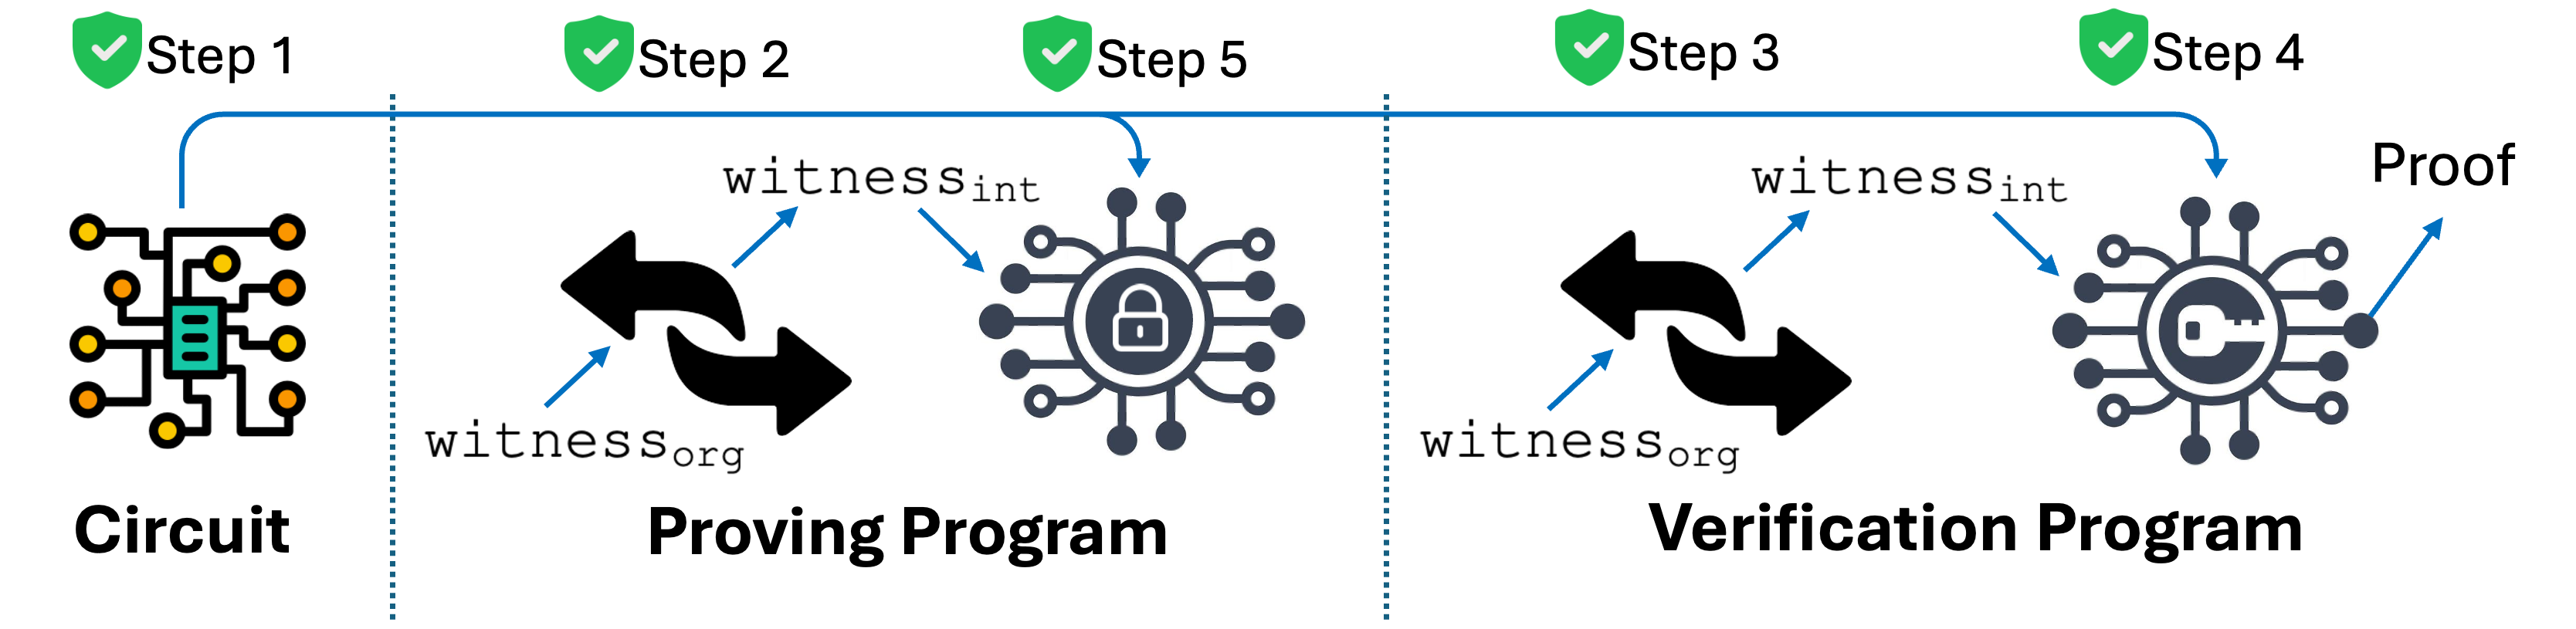
\includegraphics[width=\columnwidth,keepaspectratio]{./ch-greybox/figure/error_locator.png}
  \caption{Error localization procedure in \greyboxfuzz.}
  \label{fig:error_locator}
\end{figure}

\subsection{Error Model}

As discussed in \autoref{subsec:structure_zkp}, a \zksnark application contains two complete programs: the prover-side program \pprog and the verifier-side program \vprog. The prover-side program parses the original witness \witnessorg, converts it into the internal witness representation \witnessint, and invokes \pfunc to generate a proof. The verifier-side program parses the proof and public input, converts the public input into the internal representation expected by the verifier, and invokes \vfunc to output an accept or reject result.

The circuit itself may also be incorrect. The circuit defines the arithmetic constraints that the proof system enforces. If the circuit does not correctly represent the intended statement, then even a correct prover and verifier may produce a result that disagrees with the statement-level oracle. Therefore, \greyboxfuzz considers five possible error locations:

\begin{itemize}[leftmargin=*]
    \setlength{\itemsep}{0pt}
    \setlength{\parskip}{0pt}
    \item the circuit that encodes the intended statement;
    \item the prover-side input converter that transforms \witnessorg into \witnessint;
    \item the core proving function \pfunc;
    \item the verifier-side public-input converter;
    \item the core verification function \vfunc.
\end{itemize}

The goal of the error locator is not to prove the global correctness of all components. Instead, for a seed that already exposes an inconsistency, the error locator performs a sequence of checks to identify the first component that can explain the mismatch.

\subsection{Identifying Prover and Verifier Components}

Before \greyboxfuzz can localize an error, it must identify the component boundaries inside \pprog and \vprog. Since \greyboxfuzz targets binary programs, this step cannot rely on source-code annotations.

If the target programs dynamically link against a \zksnark library, such as \libsnark or \bellman, \greyboxfuzz can identify \pfunc and \vfunc through imported symbols, dynamic-library calls, and argument patterns. In this case, the call boundary between application code and cryptographic library code provides a natural point for extracting intermediate values.

If the target programs statically link the \zksnark library, the proving and verification functions are compiled into the same binary as the surrounding application logic. In this case, \greyboxfuzz uses the static taint tracking technique described in \autoref{subsec:branch_identify} to infer the locations of \pfunc and \vfunc.

For \pprog, \greyboxfuzz treats the circuit, \witnessorg, and proving key as taint sources. The prover-side input converter transforms \witnessorg into \witnessint, and \pfunc consumes \witnessint together with the circuit and proving key to produce a proof. Therefore, \greyboxfuzz identifies \pfunc by searching for a function that satisfies the following conditions:

\begin{itemize}[leftmargin=*]
    \setlength{\itemsep}{0pt}
    \setlength{\parskip}{0pt}
    \item It receives the circuit or circuit-derived data;
    \item It receives the proving key;
    \item It receives \witnessint, which is tainted from \witnessorg;
    \item It produces a proof object or proof-derived output.
\end{itemize}

For \vprog, \greyboxfuzz treats the proof, public input, and verification key as taint sources. The verifier-side public-input converter transforms the public input into the internal representation required by \vfunc. Then, \vfunc checks the proof using the verification key and the converted public input. Therefore, \greyboxfuzz identifies \vfunc by searching for a function that satisfies the following conditions:

\begin{itemize}[leftmargin=*]
    \setlength{\itemsep}{0pt}
    \setlength{\parskip}{0pt}
    \item It receives the verification key;
    \item It receives the proof;
    \item It receives the internal representation of the public input;
    \item It returns the accept or reject result.
\end{itemize}

After identifying these component boundaries, \greyboxfuzz hooks the corresponding program locations and extracts the intermediate values required for localization.

\subsection{Localization Procedure}

The error locator is invoked only after differential fuzzing detects a mismatch. For each generated seed, \greyboxfuzz first evaluates the intended statement using the Charm-based oracle described in \autoref{sec:differential}. It then executes the target \pprog and \vprog and compares the target verification result with the oracle result. If the two results match, the seed does not trigger localization. If the two results differ, \greyboxfuzz applies the sequential localization procedure shown in \autoref{fig:error_locator}.

The procedure checks possible error sources in the following order:

\begin{itemize}[leftmargin=*]
    \setlength{\itemsep}{0pt}
    \setlength{\parskip}{0pt}
    \item \textbf{Step 1}: Check whether the circuit correctly represents the intended statement.
    \item \textbf{Step 2}: Evaluate the circuit using the prover-side internal witness.
    \item \textbf{Step 3}: Compare the prover-side and verifier-side representations of public inputs.
    \item \textbf{Step 4}: Compare \vfunc with an independent verification implementation.
    \item \textbf{Step 5}: If all previous checks pass, attribute the remaining inconsistency to \pfunc.
\end{itemize}

This order is important. The circuit is checked first because an incorrect circuit can make all later components appear inconsistent with the intended statement. The prover-side witness conversion is checked next because \pfunc depends on the converted witness. The verifier-side public-input conversion is then checked because the verifier may interpret the public input differently from the prover. Finally, \vfunc is checked against an independent verifier. If none of these components explains the mismatch, the remaining likely source is \pfunc.

\subsection{Step 1: Circuit Validation}
\label{subsec:locate_circuit}

The first step checks whether the circuit correctly encodes the intended statement. A circuit is the constraint representation used by the proof system. It defines the arithmetic relations that must be satisfied for a proof to be valid. If the circuit is under-constrained, over-constrained, or inconsistent with the intended statement, then the program may produce proofs that are valid for the circuit but invalid for the statement the developer intended to enforce.

When existing circuit-analysis tools are applicable, \greyboxfuzz uses them to check the circuit against the intended statement. For example, tools such as Picus and ConstraintChecker can help identify circuit-level problems, including missing constraints or inconsistencies between the circuit and the expected computation. If this check shows that the circuit does not correctly represent the statement, \greyboxfuzz attributes the mismatch to the circuit rather than to \pprog or \vprog.

\subsection{Step 2: Prover-Side Witness Conversion}

If the circuit passes validation, \greyboxfuzz checks whether the prover-side input converter correctly transforms \witnessorg into the internal witness representation for the current seed. In a \zksnark program, the original witness may be represented as application-level values, such as integers, byte strings, group elements, or encoded objects. Before proof generation, these values must be converted into the representation expected by the circuit, typically finite-field elements.

\greyboxfuzz hooks \pprog after the prover-side conversion step and extracts the internal witness. It then evaluates the circuit directly using this extracted witness. If the circuit evaluation result differs from the Charm oracle result, then the extracted witness does not correctly represent the original input with respect to the intended statement. Since Step~1 has already checked the circuit, this mismatch indicates that the prover-side input converter produced an incorrect internal witness for the current seed.

This step localizes errors such as incorrect parsing, wrong field encoding, missing range conversion, endian mismatch, sign-handling errors, or inconsistent mapping from application-level values to field elements.

\subsection{Step 3: Verifier-Side Public-Input Conversion}

The verifier does not receive the prover's private witness. Therefore, \greyboxfuzz does not compare the full private witness representation between \pprog and \vprog. Instead, this step checks the public inputs, which are used by both the prover and verifier.

The prover and verifier may be developed by different parties or built using different libraries. Even if the prover-side conversion is correct for the current seed, the verifier-side converter may parse or encode the same public input differently. In that case, the verifier may check the proof against a different internal public input from the one used during proof generation.

To detect this class of error, \greyboxfuzz extracts the prover-side internal representation of the public inputs and compares it with the verifier-side internal representation of the same public inputs. If the two representations differ, \greyboxfuzz attributes the mismatch to the verifier-side public-input converter. This indicates that \vprog failed to convert the public input into the representation expected by \vfunc.

This step localizes errors such as inconsistent public-input encoding, different field-element serialization, incorrect modulus handling, and parsing differences between prover-side and verifier-side programs.

\subsection{Step 4: Verification Function Checking}

If the circuit and input converters are consistent, \greyboxfuzz checks the core verification function \vfunc. This step determines whether the verifier's cryptographic computation produces the correct accept or reject result for the proof, public input, and verification key.

The verification function in a \zksnark protocol is much simpler than the proving function. While proof generation depends on the witness, circuit, proving key, and protocol-specific randomness, proof verification mainly consists of elliptic-curve operations, scalar operations, and pairing checks over the verification key, public input, and proof. This structure makes the verifier a practical target for independent reimplementation.

A straightforward way to build this independent verifier is to use a trusted cryptographic library such as \texttt{py\_ecc}. Given the proof, verification key, and converted public input, the \texttt{py\_ecc}-based verifier recomputes the expected pairing equation and returns an accept or reject result. \greyboxfuzz then compares this result with the output of \vfunc in the target binary. If the two results differ, the inconsistency indicates that the verifier implementation in the target binary may be incorrect. This approach is useful because it avoids the need to reimplement the entire \zksnark system. It only requires an independent implementation of the verification equation for the selected curve and proof system.

However, an implementation based on a standard cryptographic library still relies on the correctness of that library and of our verifier implementation. To provide stronger confidence, \greyboxfuzz can replace the \texttt{py\_ecc}-based verifier with a formally verified verifier when the required curve and operations are supported. We build this verified verifier using HACL*, a formally verified cryptographic library developed as part of the Project Everest \cite{zinzindohoue2017hacl, project_everest}. HACL* is implemented in F* and provides verified implementations of cryptographic primitives, including elliptic-curve operations~\cite{zinzindohoue2016verified}. By building the verifier on top of verified cryptographic components, \greyboxfuzz obtains a higher-assurance reference implementation for checking \vfunc.

The formally verified verifier does not attempt to verify the entire \zksnark application or the full proving algorithm. Instead, it focuses on the verification computation, which is the part of the protocol used by \greyboxfuzz to distinguish verifier-side errors from prover-side errors. For a given proof instance, the verified verifier checks that the pairing equation and related elliptic-curve computations are performed according to the expected verification algorithm. The output of this verified implementation is then used as the reference result for \vfunc. If the target binary verifier disagrees with the verified verifier, \greyboxfuzz attributes the inconsistency to the verification function.

This design has two benefits. First, it provides a practical verifier oracle that can be used even when source code is unavailable. Second, when the HACL*-based backend is available, the oracle has stronger assurance than a conventional library-based implementation because the underlying cryptographic operations are formally verified. This improves the reliability of the error locator: a mismatch between \vfunc and the verified verifier is less likely to be caused by an error in the oracle itself.

The current limitation is curve and protocol support. A verified verifier must be implemented for the specific elliptic curve and verification equation used by the target \zksnark program. HACL* supports only a limited set of elliptic-curve operations, so not every target can use the formally verified backend. When the required curve or pairing operation is not supported, \greyboxfuzz falls back to the \texttt{py\_ecc}-based verifier. Although this fallback provides lower assurance than the formally verified implementation, it still offers an independent reference for localizing errors in \vfunc. Expanding the verified backend to support more curves and proof systems is part of our future work.

\subsection{Step 5: Final Verification}

If all previous checks pass, \greyboxfuzz attributes the remaining inconsistency to the core proving function \pfunc. At this point, the circuit has been checked against the intended statement, the prover-side witness conversion has been checked for the current seed, the verifier-side public-input conversion agrees with the prover-side representation, and the verifier computation agrees with an independent verifier.

Under these conditions, the remaining component that can explain the mismatch is the proof-generation function. This indicates that \pfunc may have generated an incorrect proof, used the wrong internal values, mishandled protocol randomness, or deviated from the expected proving algorithm.

This final step uses exclusion rather than direct full verification of the prover. This design is intentional because proof generation is substantially more complex than verification, and developing a fully independent or formally verified prover for every target setting would be expensive. By eliminating the other components first, \greyboxfuzz can still provide useful localization feedback and identify \pfunc as the most likely source of the detected inconsistency.
\section{Evaluation}
\label{sec:evaluation}

We evaluate \greyboxfuzz with three goals. First, we measure whether the input formatter can generate structured seeds at a practical speed. Second, we evaluate whether the static taint tracking component can correctly identify cryptographic branches that should be prioritized by the coverage monitor. Third, we evaluate whether \greyboxfuzz can detect cryptographic logic errors in real-world \zksnark applications more efficiently than a baseline differential fuzzing approach.

All experiments were conducted on an Intel Core i7-8700 CPU @ 3.20 GHz with 32 GB of RAM, running 64-bit Ubuntu 22.04 LTS. Unless otherwise stated, each experiment was repeated under the same configuration, and we report the average result.

\subsection{Seed Generation}

The first experiment evaluates the seed-generation efficiency of \greyboxfuzz. Since \greyboxfuzz uses an input formatter to construct seeds that follow the expected input structure of \zksnark programs, this experiment examines whether the formatting process introduces significant runtime overhead. In \greyboxfuzz, the seed structure is derived from the Charm statement provided by the user. Therefore, this experiment evaluates whether Charm-based input information can be used to generate structured seeds at a practical speed.

We compare \greyboxfuzz with \afl on three \zksnark applications: Circom Sudoku \cite{circom_sudoku}, The Age of Navigation \cite{age_of_navigation}, and dapp-zkatm \cite{dapp_zkatm}. For each tool, we measure the total number of generated seeds and the number of malformed seeds under two time budgets, 30 seconds and 60 seconds. A seed is considered malformed if it does not satisfy the expected input format of the target application. This experiment focuses on the cost and quality of seed construction before analyzing the deeper program logic explored by the fuzzer.

\autoref{tab:seed_generation} summarizes the results. Across all three applications, \greyboxfuzz generates slightly fewer seeds than \afl, but the difference is moderate. For example, within 30 seconds, \afl generates 65,906 seeds for Circom Sudoku, while \greyboxfuzz generates 53,827 seeds. Similarly, for The Age of Navigation and dapp-zkatm, \greyboxfuzz generates 55,167 and 55,251 seeds, compared with 68,704 and 68,159 seeds generated by \afl. The same trend is observed under the 60-second budget. These results show that the Charm-based formatter introduces some additional overhead, but the generation speed remains practical.

More importantly, \greyboxfuzz substantially reduces the malformed seed rate. For \afl, the malformed rate is extremely high across all applications, ranging from 94.04\% to 99.98\%. This is because \afl mutates raw bytes without knowledge of the structured input constraints required by \zksnark applications. In contrast, \greyboxfuzz keeps the malformed rate below 5\% in all settings. For example, under the 60-second budget, the malformed rates of \greyboxfuzz are 3.94\% for Circom Sudoku, 3.91\% for The Age of Navigation, and 4.62\% for dapp-zkatm. This indicates that \greyboxfuzz can preserve the expected input structure much more effectively than \afl.

Overall, the results show that \greyboxfuzz trades a small amount of seed-generation speed for a large improvement in seed validity. This tradeoff is beneficial for \zksnark application fuzzing because malformed seeds are more likely to trigger shallow parsing or format-checking failures, while well-formed seeds allow the fuzzer to reach deeper logic related to \zksnark verification and application-level constraints. Therefore, even though \greyboxfuzz generates seeds slightly more slowly than \afl, it provides better effective fuzzing performance by focusing more executions on structurally valid inputs and reducing time spent on trivial malformed-input failures.


\begin{table}[!htp]
\centering
\makebox[\textwidth][c]{%
\rotatebox{90}{
\begin{adjustbox}{max width=0.9\textheight, max totalheight=0.9\textwidth, keepaspectratio}
\begin{minipage}{\textheight}
\centering
\footnotesize
\renewcommand{\arraystretch}{1.75}
\begin{tabular}{cc|ccc|ccc}
\hline
\multicolumn{2}{c|}{\multirow{2}{*}{Execution Time}} & \multicolumn{3}{c|}{30 Seconds} & \multicolumn{3}{c}{60 Seconds} \\ \cline{3-8} 
\multicolumn{2}{c|}{} & \multicolumn{1}{c|}{\begin{tabular}[c]{@{}c@{}}Number of\\ Total Seeds\end{tabular}} & \multicolumn{1}{c|}{\begin{tabular}[c]{@{}c@{}}Number of\\ Malformed Seed\end{tabular}} & Malformed Rate & \multicolumn{1}{c|}{\begin{tabular}[c]{@{}c@{}}Number of\\ Total Seeds\end{tabular}} & \multicolumn{1}{c|}{\begin{tabular}[c]{@{}c@{}}Number of\\ Malformed Seed\end{tabular}} & Malformed Rate \\ \hline
\multicolumn{1}{c|}{\multirow{3}{*}{AFL}} & Circom Sudoku & \multicolumn{1}{c|}{65906} & \multicolumn{1}{c|}{65888} & 99.97\% & \multicolumn{1}{c|}{112729} & \multicolumn{1}{c|}{112711} & 99.98\% \\ \cline{2-8} 
\multicolumn{1}{c|}{} & The Age of Navigation & \multicolumn{1}{c|}{68704} & \multicolumn{1}{c|}{66801} & 97.23\% & \multicolumn{1}{c|}{134908} & \multicolumn{1}{c|}{131114} & 97.19\% \\ \cline{2-8} 
\multicolumn{1}{c|}{} & dapp-zkatm & \multicolumn{1}{c|}{68159} & \multicolumn{1}{c|}{64102} & 94.04\% & \multicolumn{1}{c|}{134492} & \multicolumn{1}{c|}{127209} & 94.58\% \\ \hline
\multicolumn{1}{c|}{\multirow{3}{*}{\greyboxfuzz}} & Circom Sudoku & \multicolumn{1}{c|}{53827} & \multicolumn{1}{c|}{2195} & 4.08\% & \multicolumn{1}{c|}{101983} & \multicolumn{1}{c|}{4018} & 3.94\% \\ \cline{2-8} 
\multicolumn{1}{c|}{} & The Age of Navigation & \multicolumn{1}{c|}{55167} & \multicolumn{1}{c|}{2147} & 3.89\% & \multicolumn{1}{c|}{106727} & \multicolumn{1}{c|}{4175} & 3.91\% \\ \cline{2-8} 
\multicolumn{1}{c|}{} & dapp-zkatm & \multicolumn{1}{c|}{55251} & \multicolumn{1}{c|}{2692} & 4.87\% & \multicolumn{1}{c|}{104940} & \multicolumn{1}{c|}{4851} & 4.62\% \\ \hline
\end{tabular}

\caption{Seed- generation speed and malformed rate comparison among \afl and \greyboxfuzz under different time budgets.}
\label{tab:seed_generation}
\end{minipage}
\end{adjustbox}%
}%
}
\end{table}




% \begin{table*}[t]
% \centering
% \begin{tabular}{cc|ccc|ccc}
% \hline
% \multicolumn{2}{c|}{\multirow{2}{*}{Execution Time}} & \multicolumn{3}{c|}{30 Seconds} & \multicolumn{3}{c}{60 Seconds} \\ \cline{3-8} 
% \multicolumn{2}{c|}{} & \multicolumn{1}{c|}{\begin{tabular}[c]{@{}c@{}}Number of\\ Total Seeds\end{tabular}} & \multicolumn{1}{c|}{\begin{tabular}[c]{@{}c@{}}Number of\\ Malformed Seed\end{tabular}} & Malformed Rate & \multicolumn{1}{c|}{\begin{tabular}[c]{@{}c@{}}Number of\\ Total Seeds\end{tabular}} & \multicolumn{1}{c|}{\begin{tabular}[c]{@{}c@{}}Number of\\ Malformed Seed\end{tabular}} & Malformed Rate \\ \hline
% \multicolumn{1}{c|}{\multirow{3}{*}{AFL}} & Circom Sudoku & \multicolumn{1}{c|}{65906} & \multicolumn{1}{c|}{65888} & 99.97\% & \multicolumn{1}{c|}{112729} & \multicolumn{1}{c|}{112711} & 99.98\% \\ \cline{2-8} 
% \multicolumn{1}{c|}{} & The Age of Navigation & \multicolumn{1}{c|}{68704} & \multicolumn{1}{c|}{66801} & 97.23\% & \multicolumn{1}{c|}{134908} & \multicolumn{1}{c|}{131114} & 97.19\% \\ \cline{2-8} 
% \multicolumn{1}{c|}{} & dapp-zkatm & \multicolumn{1}{c|}{68159} & \multicolumn{1}{c|}{64102} & 94.04\% & \multicolumn{1}{c|}{134492} & \multicolumn{1}{c|}{127209} & 94.58\% \\ \hline
% \multicolumn{1}{c|}{\multirow{3}{*}{\greyboxfuzz}} & Circom Sudoku & \multicolumn{1}{c|}{53827} & \multicolumn{1}{c|}{2195} & 4.08\% & \multicolumn{1}{c|}{101983} & \multicolumn{1}{c|}{4018} & 3.94\% \\ \cline{2-8} 
% \multicolumn{1}{c|}{} & The Age of Navigation & \multicolumn{1}{c|}{55167} & \multicolumn{1}{c|}{2147} & 3.89\% & \multicolumn{1}{c|}{106727} & \multicolumn{1}{c|}{4175} & 3.91\% \\ \cline{2-8} 
% \multicolumn{1}{c|}{} & dapp-zkatm & \multicolumn{1}{c|}{55251} & \multicolumn{1}{c|}{2692} & 4.87\% & \multicolumn{1}{c|}{104940} & \multicolumn{1}{c|}{4851} & 4.62\% \\ \hline
% \end{tabular}
% \caption{Seed- generation speed and malformed rate comparison among \afl and \greyboxfuzz under different time budgets.}
% \label{tab:seed_generation}
% \end{table*}



\subsection{Coverage Evaluation}

The second experiment evaluates the effectiveness of the coverage monitor. As discussed in Section~\ref{sec:coverage_monitor}, \greyboxfuzz uses static taint tracking to identify cryptographic branches before fuzzing begins. The purpose of this experiment is to determine whether the taint tracker can correctly identify branches related to proof generation and proof verification.

We use \rapidsnark as the target library for this evaluation. \rapidsnark is a C++ implementation of \zksnark proof generation and verification for circuits produced by Circom and snarkjs. It is a suitable target because it contains both prover and verifier components and is used in practical \zksnark workflows. To construct a reliable ground truth, we compiled \rapidsnark version v0.0.8 with debugging information enabled. This allows us to correlate assembly instructions with source-code locations and manually determine whether each branch belongs to cryptographic computation or general program logic.

After compilation, we extracted the assembly code of the prover and verifier and manually labeled each branch as either a cryptographic branch or a non-cryptographic branch. A branch is labeled as cryptographic if it directly participates in proof generation, proof verification, witness processing, finite-field arithmetic, elliptic-curve computation, or pairing-related computation. Branches related only to parsing, file handling, memory management, logging, or other general program functionality are labeled as non-cryptographic. This manual labeling serves as the ground truth for evaluating the static taint tracking result.

We then ran the static taint tracker on the same \rapidsnark binaries. The taint tracker automatically marks branches that are influenced by cryptographic inputs, such as the circuit, witness, proving key, proof, public input, and verification key. We compare the automatically tainted branches with the manually labeled ground truth. \autoref{tab:coverage_performance} reports the number of branches in each component, the number of branches marked by static taint tracking, and the correctness of the classification.

The main goal of this evaluation is to measure whether \greyboxfuzz can identify cryptographic branches with high coverage. Missing cryptographic branches is more harmful than marking a small number of non-cryptographic branches, because missed cryptographic branches may prevent the fuzzer from exploring security-relevant computation. In contrast, a small number of false positives only causes \greyboxfuzz to monitor additional branches. Therefore, this evaluation focuses on whether the taint tracker successfully captures the cryptographic branches needed for guiding fuzzing.


The results show that static taint tracking can effectively identify the cryptographic branches needed by the coverage monitor. Only 14 out of 250 \cryptobranch branches (5.6\%) are not successfully identified by the taint tracker, which means that \greyboxfuzz captures most branches related to proof generation and proof verification. Meanwhile, 36 out of 239 \programbranch branches (15.1\%) are incorrectly identified as \cryptobranch branches. However, these false positives do not cause \greyboxfuzz to miss critical vulnerabilities. Instead, they only cause \greyboxfuzz to monitor a small number of additional branches. Since most cryptographic branches are correctly tainted and only a limited number of non-cryptographic branches are misclassified, \greyboxfuzz can guide fuzzing toward proof-related computation without introducing significant unnecessary overhead.



\begin{table*}[!t]
\centering
\footnotesize
\renewcommand{\arraystretch}{1.15}
\begin{tabular}{c|c|ccc|cc}
\toprule
Branch Type & Total Branch & Tainted & Untainted & Mis-Tainted & Error Rate & Correct Rate \\
\midrule
Cryptographic & 250 & 236 & 14 & 14 & 5.6\% & 94.4\% \\
\midrule
Non-cryptographic & 239 & 36 & 203 & 36 & 15.1\% & 84.9\% \\
\midrule
Overall & 489 & 272 & 217 & 50 & 10.2\% & 89.8\% \\
\bottomrule
\end{tabular}
\caption{Coverage evaluation of static taint tracking on \rapidsnark.}
\label{tab:coverage_performance}
\end{table*}


\subsection{Performance Evaluation}

After demonstrating the seed-generation speed and coverage performance of \greyboxfuzz, we run a third experiment to evaluate its bug detection performance. We selected a set of \zksnark applications from both real-world projects and known vulnerability patterns. The selected programs include common circuit-level mistakes, application-level input validation bugs, and implementation errors that may cause a verifier to accept an invalid proof or reject a valid proof.

We selected \zksnark applications from different sources, including prototype demos, academic projects, and live applications. These applications are implemented in different programming languages, including C, Rust, and Go, and are built on different \zksnark frameworks and tools, including \rapidsnark, \bellman, \arkworks, \circom, \gnark, and \snarkjs. This diversity allows us to evaluate \greyboxfuzz under a wide range of implementation settings and demonstrates that \greyboxfuzz is not limited to a specific programming language, framework, or development workflow.


\autoref{tab:bug_evaluation} presents the bugs identified in the tested applications. Because \greyboxfuzz includes an error locator, the table also reports the component that caused the detected bug. This additional information helps developers determine whether the issue comes from the circuit, prover-side conversion, proof generation, verifier-side conversion, or verification.

\begin{table*}[!t]
\centering
\small
\renewcommand{\arraystretch}{1.25}
\begin{tabular}{p{0.37\textwidth}|p{0.13\textwidth}|p{0.11\textwidth}|p{0.14\textwidth}|p{0.11\textwidth}}
\hline
\textbf{Error/Vulnerability in \zksnark Program} 
& \textbf{Library} 
& \textbf{Protocol} 
& \textbf{Location} 
& \textbf{Bug Type} \\ \hline\hline

\multicolumn{5}{c}{\textbf{Potentially Locatable in Current Libraries}} \\ \hline

Multiple Gadget Conflict Issue 
& All libraries 
& R1CS 
& Circuit 
& Common \\ \hline

Incorrect Bit/Comparison Gadget Implementation 
& \libsnark 
& R1CS 
& Circuit 
& Common \\ \hline

Developer Incorrect Flattening 
& All libraries 
& R1CS 
& Circuit 
& Common \\ \hline

BigInt: Missing Bit Length Check
& All libraries 
& R1CS 
& Circuit 
& Common \\ \hline

Arithmetic Over/Under Flows 
& Circom 
& R1CS 
& Circuit 
& Common \\ \hline\hline

\multicolumn{5}{c}{\textbf{Bugs in the Wild}} \\ \hline

Unused Variables Issues in Circuit 
& gnark 
& Groth16 
& Setup/Prover 
& Real-world \\ \hline

\zksnark in Federated Learning
& Circom 
& Groth16 
& Circuit 
& Real-world \\ \hline

\end{tabular}
\caption{Error and vulnerability cases used to evaluate the error localization capability of \greyboxfuzz.}
\label{tab:bug_evaluation}
\end{table*}

The expected benefit of \greyboxfuzz comes from three design choices. First, the input formatter generates structured seeds that are more likely to reach proof generation and verification. Second, the coverage monitor prioritizes seeds that exercise new cryptographic branches instead of treating all execution paths equally. Third, the error locator provides component-level feedback after a mismatch is detected. Together, these features allow \greyboxfuzz to detect cryptographic logic errors more efficiently than a general differential fuzzing baseline.


In Section~\ref{sec:discussion}, we further discuss selected security bugs discovered during the evaluation and explain how the error locator helps identify their causes.
\section{Discussion}
\label{sec:discussion}

In this section, we will discuss selected issue that \greyboxfuzz discover during the evaluation process


\subsection{Unused Variables Issues in Circuit}



Unused public variables may introduce a security risk when a value is declared as a public input and is expected by the verifier to be part of the proved statement, but the circuit does not enforce the intended relationship for that value. Public inputs are visible to the verifier and are commonly used to represent externally checked values, such as an identity commitment, a balance, a nullifier, an output value, or an application-specific parameter. If such a value is declared but not properly connected to the circuit constraints, the verifier may believe that the proof guarantees a statement involving that value, while the circuit proves only a weaker statement. For example, suppose a circuit is intended to prove that a user is older than 18, and the public input is the claimed age. If the circuit declares \texttt{age} as public but only proves knowledge of a private secret and never constrains \texttt{age}, then a malicious prover can generate a valid proof with \texttt{age = 25}, even though the witness does not establish that the user is older than 18. From the verifier's perspective, the proof appears to be associated with the public value \texttt{25}; however, the circuit never checks the age condition. This is not necessarily a failure of proof generation or proof verification. Instead, it is a mismatch between the statement the verifier believes is being proven and the actual constraints enforced by the circuit. The impact can be severe when the unused public variable controls authorization, asset ownership, eligibility, or other security-critical application logic, because an attacker may produce a proof that verifies successfully while bypassing the intended public-input condition.


Currently, \circom can successfully compile a circuit with an unused public variable, and the compiler does not automatically enforce that every public input appears in the intended constraints. This can be dangerous if the proof system does not bind each declared public input to the generated proof, because an attacker may generate a proof for one public input and then reuse the same proof with a different public input. Libraries commonly used with \circom, such as \snarkjs and \rapidsnark, address this input-consistency soundness issue in the R1CS-to-QAP reduction. As described in Remark~2.5 of \cite{ben2014succinct}, some R1CS instances can produce QAP polynomials that are distinct but not linearly independent. The fix increases the QAP degree from \texttt{cs.num\_constraints()+1} to \texttt{cs.num\_constraints()+cs.num\_inputs()+1}, ensuring that public-input polynomials remain independent. Therefore, even if a public variable is unused in the original circuit constraints, the proof is still bound to that declared public input, preventing an attacker from changing the public input after proof generation without invalidating the proof.

Similar fixes have also been adopted by other \zksnark libraries, including \libsnark, \bellman, and \arkworks. However, during our evaluation, \greyboxfuzz found that the unused public variable issue still exists in \playsnark and \gnark \cite{consensys_gnark}. \playsnark is a playground for learning \zksnark proof systems and is not intended for secure deployment. In contrast, \gnark is a production-oriented library that has undergone security audits, but it currently does not follow the R1CS-to-QAP transformation described in Remark~2.5 of \cite{ben2014succinct}. As a result, if an unused public variable exists in the circuit, the generated proof may not be fully bound to that public input. A malicious prover can generate a proof using one public value and then replace that value with another public value during verification, while the verifier may still accept the proof.


\subsection{\zksnark in Federated Learning}
In this work~\cite{han2023kick}, zkSNARKs are used to make the anomaly-detection process in federated learning verifiable. The server acts as the prover and the clients act as verifiers. After the server runs the anomaly-detection mechanism and removes suspected malicious clients, it generates a zkSNARK proof showing that the detection and removal steps were executed correctly. Clients can then verify this proof without redoing the full computation and without relying only on the server's claim. The paper uses zkSNARKs because they provide small proofs and fast verification, which is important when federated-learning clients have limited resources.

The paper uses \zksnark to prove that the server correctly executes the anomaly-detection computation in federated learning. This computation includes several numerical operations, such as matrix multiplication, cosine similarity, division, and square root. Since square root is expensive and difficult to compute directly inside an arithmetic circuit, the paper asks the prover to provide the square-root result \(x\) as a witness and then checks the relationship between \(x\) and the input value \(y\). Instead of computing \(x=\sqrt{y}\) inside the circuit, the circuit checks whether \(x^2 \leq y\) and \((x+1)^2 \geq y\). This design reduces the square-root verification cost to two multiplications and two comparisons.

However, this condition does not exactly prove that \(x\) is the correct integer square root of \(y\). For example, when \(y=9\), the correct square root is \(x=3\), but \(x=2\) also satisfies \(2^2 \leq 9\) and \((2+1)^2 \geq 9\). Therefore, the circuit may accept an incorrect square-root witness for perfect-square values. This is a circuit correctness issue and may become a security issue if the square-root value affects a threshold, distance, standard deviation, anomaly score, or final detection decision. In this paper, the square-root value is used as part of an approximate numerical computation for anomaly detection, so an off-by-one error may have limited impact if the final decision is not sensitive to small numerical changes. However, if a client model is close to the decision boundary, or if the square-root result is used in a threshold-sensitive computation, this approximation may change the anomaly-detection result and should not be considered fully sound.

For this specific application, the \zksnark proof may not require full numerical accuracy because the federated-learning model and anomaly-detection process already tolerate some deviation in model updates and statistical measurements. However, from the cryptographic perspective, the circuit still cannot fully represent the original statement that it intends to prove. Therefore, this issue should be understood as a circuit-level approximation error: it may be acceptable for this particular machine-learning application if it does not affect the final classification result, but it would be unsafe in applications where the square-root value is used in exact security-critical logic.


\section{Future Work}

In general, \greyboxfuzz was designed and developed based on the \zksnark protocol. However, most of its components are not specifically tailored for \zksnark alone and can be extended to support other \zkp protocols. In this section, we discuss the possible extensions of \greyboxfuzz and evaluate its applicability by running several programs on different \zkp protocols.

As presented in \autoref{sec:overview}, \greyboxfuzz consists of four major components: differential fuzzing ground truth, input formatter, coverage monitor, and error locator. The differential fuzzing ground truth and input formatter are designed using Charm, which facilitates cryptographic variable handling in \zkp statements. These components are not tied to a single \zksnark protocol but can represent any cryptographic statement in a \zkp protocol. As a result, no additional implementation or design modifications are required to extend \greyboxfuzz to support differential fuzzing ground truth and input formatting for other \zkp protocols.

The coverage monitor analyzes the binary program and classifies assembly instructions into \cryptobranch and \programbranch using our taint tracking tool. The taint tracking strategy classifies any variable that correlates with input variables as tainted. If this strategy can be applied to another \zkp protocol, no additional implementation is needed for the coverage monitor. For instance, in Bulletproofs, a non-interactive \zkp protocol with short proofs and no trusted setup, the prover takes the circuit, witness, Pedersen commitments, and public parameters (such as $G$ and $H$) as input. The same taint tracking strategy used for \zksnark can be applied to classify \cryptobranch in Bulletproofs since all variables computed based on protocol inputs fall into this category. We believe that most \zkp protocols can adopt a similar strategy to identify \cryptobranch and \programbranch without requiring modifications.

The error locator, which helps identify errors in \zkp programs, requires protocol-specific implementations. A universal error locator is not available for multiple \zkp protocol. However, since the error locator is an optional component of \greyboxfuzz, its absence does not prevent the fuzzer from detecting errors and security vulnerabilities in \zkp binary programs. Thus, even without implementing a dedicated error locator for each \zkp protocol, \greyboxfuzz can still be extended to other \zkp protocols, as all other core components do not require protocol specific modifications.
\chapter{CONCLUSION \& FUTURE WORK}
\label{ch:conclusion}
Cryptographic implementations connect the mathematical design of a protocol with the behavior of deployed systems. A cryptographic protocol may be mathematically sound, but its real-world security depends on whether the implementation correctly realizes the intended computation, whether security-critical cryptographic code can be identified, and whether testing methods can expose implementation-level errors before deployment. The works presented in this dissertation advance these goals by developing systematic evaluation, automated checking, and binary-level testing techniques for cryptographic software.

The first contribution studies cryptographic function identification in binaries and provides a comprehensive evaluation of existing approaches for detecting cryptographic algorithms in compiled programs. This work conducts reproduction and replication studies, organizes the design space of existing tools, and develops a noval benchmarking framework that supports more consistent comparison across different approaches. The evaluation covers modern cryptographic algorithms, microbenchmarks, libraries, and large applications, while also accounting for practical variations introduced by compilers, optimization levels, obfuscation strategies, operating systems, and algorithm versions. This work clarifies the current state of cryptographic function identification, including major existing gaps and key directions for future work, and provides a benchmark foundation for evaluating future detection techniques in a more systematic and reproducible manner.

The second contribution introduces \snarkprobe, an automated security analysis framework for zkSNARK implementations. \snarkprobe targets cryptographic logic errors that are difficult to detect through ordinary testing. Rather than only checking for crashes or successful proof generation, it determines whether an implementation is consistent with the expected proof statement. By identifying inconsistencies across the constraint system, witness generation, and verification logic, \snarkprobe reduces the manual effort required to analyze complex zkSNARK implementations and provides a practical framework for improving confidence in zero-knowledge proof software. \snarkprobe currently supports two zkSNARK protocols, Pinocchio and Groth16, and has been evaluated on several libraries. It successfully detected seven security vulnerabilities and one previously reported CVE in zkSNARK libraries within practical time limits, demonstrating its effectiveness for security evaluation.

The third contribution develops \greyboxfuzz, a grey-box differential fuzzing framework for zero-knowledge proof binary applications. \greyboxfuzz addresses deployment settings in which source-level assumptions are insufficient and the executable itself must be tested. By combining structured input generation, coverage analysis, and error localization, \greyboxfuzz moves binary testing beyond general crash detection toward identifying logic-level errors in zero-knowledge proof applications. This binary-level capability makes \greyboxfuzz well suited to the practical security evaluation of deployed \zkp applications, whose source code is often unavailable. Experiments show that \greyboxfuzz achieves significantly better time performance than general-purpose fuzzing tools and detects seven security vulnerabilities in \zksnark applications, including two previously unreported vulnerabilities in \zksnark implementations, thereby helping improve the security of future cryptographic deployments.

Future work can extend these research directions in two major ways. First, the current analysis frameworks can be expanded to support a broader range of zero-knowledge proof protocols beyond zkSNARKs, such as zkSTARKs, Bulletproofs, and Plonk-based systems. Different proof systems use different arithmetization methods, transcript structures, polynomial commitment schemes, and verification procedures, so extending the analysis to these protocols would help evaluate whether similar implementation-level weaknesses appear across a wider zero-knowledge ecosystem.

Second, future work can further incorporate formal verification to provide stronger assurance for critical components of cryptographic implementations. This direction is complementary to fuzzing-based analysis because the two approaches offer different advantages. Fuzzing provides greater compatibility with real-world software artifacts and requires less protocol-specific understanding, making it practical for testing diverse implementations, deployed binaries, and systems where complete formal specifications are difficult to obtain. Formal verification, in contrast, can provide stronger correctness guarantees for selected algorithms, protocols, or components once precise specifications are available. Integrating these techniques would support a more comprehensive methodology: fuzzing can broadly test heterogeneous cryptographic software with relatively low specification requirements, while formal verification can establish stronger guarantees for security-critical components that are suitable for rigorous specification and proof.

Overall, reliable cryptographic software requires attention to the gap between intended cryptographic behavior and actual implementation behavior. Even when a protocol is well designed, implementation errors can still affect key generation, encryption, decryption, authentication, validation, data conversion, and other security-critical operations. Practical analysis techniques therefore play an important role in identifying inconsistencies that ordinary testing may miss. Strengthening these techniques can improve confidence in cryptographic software and support the development of more secure real-world systems.



% Test \begin{chapteracknowledgement}...\end{chapteracknowledgement}, etc.
%%%% \include{ch-test-miscellaneous}

% Test per-chapter references.
%%%% \include{ch-test-per-chapter-references}

\makeatletter  % commented out on 2022-01-26
  \defbibenvironment{bibliography}
    {%
      \list
        {%
          \printtext[labelnumberwidth]%
          {%
            \printfield{prefixnumber}%
            \printfield{labelnumber}%
          }%
        }%
        {%
          \setlength{\bibhang}{1in} %%%%% was 0pt
          \setlength{\itemindent}{1in}%  -\leftmargin} %%%%% was 0pt
          \setlength{\itemsep}{\bibitemsep}%
          \setlength{\leftmargin}{0pt}%  .22in} % 0.42in}
          \setlength{\parsep}{\bibparsep}%
          \setlength{\rightmargin}{0.33in}%
        }%
    }
    {\endlist}
    {\item}
\makeatother  % commented out on 2022-01-26

% \immediate\setlength{\labelnumberwidth}{1.5in} %%%%% was commented out
\setlength{\labelwidth}{1.5in}

{%
  % Make _ in URLs visible.
  % \def\t{\char'137}%
  \catcode`*=\active
  \def*{\char'137}%  \char'137 is _
  \PrintBibliography
}

% Appendices are optional.  Not all theses contain appendices.
% An appendix is used for supplementary illustrative material,
% original data, computer programs, and other material that is not
% necessarily appropriate for inclusion within the text of your
% thesis.
% Reference: TM2017 page 33.
%
% Use ``\appendix'' for one appendix or ``\appendices'' for more than
% one appendix.
\appendices

% My filename conventions:
%     FILE THAT START WITH    ARE
%     ap-                     appendices
%     ch-                     chapters
%     gr-                     graphics
%     pa-                     packages
%     z                       temporary files

  % \ProvidesFile{ap-about-appendices.tex}[2022-10-05 about the appendicies appendix]

\begin{VerbatimOut}{z.out}
\chapter{ABOUT THE APPENDICES}

% Use single spacing in the appendices from now on to save space.
% \ZZbaselinestretch{1}

\textcolor{red}{%
  \textbf{%
    These appendices are single-spaced to save space.
    Your thesis should use the default~1.5 line spacing.%
  }%
}

There are two groups of appendices.
The first group are general appendices;
the second group are domain-specific appendices.

These appendices are a series of examples.
They are a work in progress.

Each example consists of some \LaTeX\ output
followed by the corresponding input lines.
Some \LaTeX\ input lines only define things
and don't produce any output.
Each chunk in the input file begins with
\verb+\begin{VerbatimOut}{z.out}+
then has the \LaTeX\ input for the example,
% Don't literally end VerbatimOut on next line.
and ends with {\tt \char'134 end\char'173 VerbatimOut\char'175},
followed by a blank line,
followed by a line that begins with
|\My|.

\end{VerbatimOut}

\MyIO


\begin{VerbatimOut}{z.out}


\section{Paragraphs}

This is the first paragraph.
Paragraphs are separated by blank lines.

This is the second paragraph.


\section{Section Heading}

This is a sentence.
This is a sentence.
This is a sentence.
This is a sentence.
This is a sentence.


\subsection{Subsection heading}

This is a sentence.
This is a sentence.
This is a sentence.
This is a sentence.
This is a sentence.


\subsubsection{Subsubsection heading}

This is a sentence.
This is a sentence.
This is a sentence.
This is a sentence.
This is a sentence.
\end{VerbatimOut}

\MyIO



\begin{VerbatimOut}{z.out}


\section{Text math}

If items in a list are narrow like these Greek characters,\\
    \I2 \verb+$\alpha$, $\beta$, and $\gamma$+\\
I'd input the line like this\\
    \I2 \verb+$\alpha$,~$\beta$, and~$\gamma$+\\
where the \verb+~+ is a tie
that ties together what's before and after it on the same line of the output
\cite[page~92]{knuth2012}.

This text is the correct length to show what happens with and without ties:
$\alpha$,
$\beta$,
and $\gamma$.
See how the line gets split
and the~$\gamma$ is at the beginning of the line?

This text is the correct length to show what happens with and without ties:
$\alpha$,~$\beta$,
and~$\gamma$.
See how the line gets compressed a little bit so the~$\gamma$
is not at the beginning of the line?
\end{VerbatimOut}

\MyIO

  \chapter{APPENDIX FOR CHAPTER~\ref{ch:cryptobinary}}
\section{Procedure for R+R Evaluation}

\subsection{Steps in our Reproduction Evaluation}
\label{app:cryptobinary-repro_procedure}
\begin{enumerate}
\item Obtain access to each tool; compile the tool if required, following the provided instructions.
\item Set up the environment to replicate the tool's original configuration (follows the same operating conditions).
\item Obtain the original test cases for each tool. If unavailable, the reproduction evaluation will be skipped (follows the same measuring system).
\item Execute each tool with the provided test cases to reproduce the results (follows the same measurement procedure).
\end{enumerate}

\subsection{Steps in our Replication Evaluation}
\label{app:cryptobinary-repli_procedure}
\begin{enumerate}
\item Obtain access to each tool; recompile the tool on our system if the source code is available.
\item Build and run each tool on Windows 10, Ubuntu 18.04, and macOS Sonoma (follows the different measuring system).
\item Compile our custom benchmarks with the evaluation metrics into binaries for testing.
\item Execute each tool with our benchmarks to assess replication capability (follows the different location on multiple trials).
\end{enumerate}

\section{Tools}
\label{app:cryptobinary-tools}
We provide introductions to the tools analyzed in this work.  For each tool, we give a high level overview, highlight key features for a user, and provide a discussion on its strengths and weaknesses, as relevant.

\subsection{Aligot} 

\parhead{Summary.} Aligot \cite{calvet2012aligot}  is based on the assumption that the input-output relations in a cryptographic function remain unchanged
even if there is obfuscation. It performs an interloop data-flow analysis to identify cryptographic parameters and then performs a comparison
with a reference implementation. The authors successfully evaluated the tool to identify four different cryptographic functions: TEA, RC4, AES and MD5.

\parhead{Highlights for User.}
\begin{itemize}
  \item Requires the user to compile the tool with Intel Pin
  \item Requires an earlier version of Intel Pin and Python library \textit{networkx} (latest does not work)
\end{itemize}

\parhead{Other Discussion.}
\begin{itemize}
  \item Aligot has not been updated to accommodate the latest dependency changes. Specifically, the Python library "networkx" uses different data types that cause crashes in Aligot
  \item Additionally, the Aligot tracer has not been adapted to the latest version of Intel Pin, and the tested version appears to be discontinued
\end{itemize}

%%%%%%%%%%%%%%%%%%%%
\subsection{CryptoHunt} 
\parhead{Summary.} CryptoHunt \cite{xu2017cryptographic} introduces the \textit{bit-precise symbolic loop mapping} technique to identify cryptographic functions. Using this technique the tool captures the semantics of possible cryptographic algorithms within a loop and then performs guided fuzzing to efficiently match boolean formulas with known reference implementations. It shows its efficacy on commonly used cryptographic functions such as TEA, AES, RC4, MD5, and RSA under different control and data obfuscation scheme combinations.

\parhead{Highlights for User.}
\begin{itemize}
  \item Requires the user to compile the tool with Intel Pin (2.13, 3.2, and 3.28 are tested)
  \item Requires the user to indicate the reference loop
  \item Higher accuracy rate and detection results in obfuscated binaries
\end{itemize}

\parhead{Other Discussion.}
\begin{itemize}
  \item Depending on the binary program size, CryptoHunt may find 10,000 loops in the binary, which needs to be compared with the reference one by one. The long analysis time may not suitable for a large program.
\end{itemize}

%%%%%%%%%%%%%%%%%%%%
\subsection{CryptoKnight}
\parhead{Summary.} CryptoKnight \cite{hill2018cryptoknight} employs a Dynamic Convolutional Neural Network (DCNN)
to learn from variable-length control flow diagnostics output obtained from a dynamic trace, and
is able to detect AES, RC4, Blowfish, MD5, and RSA.

\parhead{Highlights for User.}
\begin{itemize}
  \item Can easily integrate new samples through the scalable synthesis of customizable cryptographic algorithms
  \item Automated and limits user interaction
  \item High accuracy rate (96\%)
\end{itemize}

\parhead{Other Discussion.}
\begin{itemize}
  \item Has been evaluated on GnuPG and a real-world ransomware binary 'GonnaCry' and can successfully identify the use of AES and RSA
\end{itemize}

%%%%%%%%%%%%%%%%%%%%
\subsection{Draft Crypto Analyzer (DRACA)}
\parhead{Summary.} DRACA ~\cite{draca} targets preliminary detection and analysis of cryptographic algorithms within executables.
Although DRACA is implemented as a command line utility for x86/Win32, it can also analyze Unix ELF binaries,
Java applets, as well as 16- and 32-bit DOS Windows executables.

\parhead{Highlights for User.}
\begin{itemize}
  \item No compiling is needed
  \item Can be directly run by passing the target binary program
\end{itemize}

\parhead{Other Discussion.}
\begin{itemize}
  \item DRACA can only provide a rough idea of what kind of algorithms to look at without actual spending time on decompilation and code analysis.
  \item Detection result cannot be used without further analysis.
\end{itemize}


%%%%%%%%%%%%%%%%%%%%
\subsection{FindCrypt2} 
\parhead{Summary.} FindCrypt2 \cite{findcrypt2} has been implemented as a plug-in support for IDA Pro~\cite{IDA_pro} which searches constants used in the initialization of cryptographic algorithms. It can detect commonly used encryption algorithms.

\parhead{Highlights for User.}
\begin{itemize}
  \item Requires IDA Pro, a commercial disassembler software, which is not free
\end{itemize}


\subsection{HCD} 
\parhead{Summary.} HCD \cite{hcd} detects roughly 90 hash and cryptographic algorithms and compiles for portable executable files with a GUI interface and Shell integration, Command line support.

\parhead{Highlights for User.}
\begin{itemize}
  \item No compiling is needed
  \item Can be directly run by passing the target binary program
\end{itemize}

\parhead{Other Discussion.}
\begin{itemize}
    \item Can only detect cryptographic functions in executable file for Microsoft Windows (.exe). This tool does not support the analysis of Unix based binary programs.
\end{itemize}

%%%%%%%%%%%%%%%%%%%%
\subsection{PEiD KANAL} 
\parhead{Summary.} PEiD KANAL \cite{kanal} is a plug-in for PEiD, searching for cryptographic algorithms with a specific signature such as fixed s-boxes, permutation tables, and initialization values. It searches for connections to identified code or data and find its associated address.

\parhead{Highlights for User.}
\begin{itemize}
  \item No compiling is needed
  \item Can be directly run by passing the target binary program
\end{itemize}

%%%%%%%%%%%%%%%%%%%%
\subsection{Signsrch} 
\parhead{Summary.}  Signsrch \cite{signsrch}  is another IDA Pro plug-in which aims to detect not just encryption algorithms, but also compression algorithms, multimedia, etc. The tool searches for known signatures as well as allows a user to add their own signature.

\parhead{Highlights for User.}
\begin{itemize}
  \item No compiling is needed
  \item Can be directly run by passing the target binary program
\end{itemize}

%%%%%%%%%%%%%%%%%%%%
\subsection{Where's Crypto} 
\parhead{Summary.} Where's Crypto \cite{meijer2021s} is an IDA SDK based tool, aiming to automatically identify cryptographic primitives in binaries. Where's Crypto can detect cryptographic functions that has as-of-yet unknown primitives if it falls within a taxonomical class of well-defined primitives.

\parhead{Highlights for User.}
\begin{itemize}
  \item Requires IDA Pro, a commercial disassembler software, which is not free
  \item Supports unknown cryptographic primitives
\end{itemize}

%%%%%%%%%%%%%%%%%%%%
%%%%%%%%%%%%%%%%%%%%

% \section{Unavailable Tools}
% \label{subsec:unavailable}
% \fanyo{Move to RR}

% While working on this systematization of the space, we discovered that certain tools were rendered inoperable due to unavailable dependencies, missing documentation, or alterations in CPU architectures since they were first developed. 

% \parhead{Aligot} is a cryptographic function identification tool developed based on Pin, a dynamic binary instrumentation framework developed by Intel. Aligot was tested with Pin 2.10 and Pin 2.12 by its developer, but unfortunately, these versions are no longer available. Consequently, we attempted to use an older version of Pin (3.22) but we were unable to execute Aligot correctly. We believe this to be due to the fact that these tool do not support and cannot be executed on recent CPU architectures.

% \parhead{CryptoHunt} has been successfully executed, but we are unable to provide the complete benchmarking framework and performance metric evaluation results. CryptoHunt detects cryptographic functions in binary code through a bit-precise symbolic loop mapping approach. However, depending on the binary's size, CryptoHunt may identify up to 10,000 loops within the binary. Without additional filtering, the process of comparing each of these loops with reference loops becomes exceedingly time-consuming and infeasible.

% \parhead{CryptoSearcher} is a cryptographic function detection tool developed in 2004, and was evaluated previously in \cite{xu2017cryptographic}. However, we cannot find the tool's source code or documentation about how to use this tool. We only found the cryptographic signature files such as Blowfish, RC2, RC4, RC5, RC6, CAST-256, etc. Currently, we cannot evaluate this tool due to the lack of tool's source program and its documentation.

% \parhead{Kerckhoff} cannot be evaluated in this paper due to the lack of tool's source code or documentation.


\chapter{APPENDIX FOR CHAPTER~\ref{ch:snarkprobe}}
% \iffalse

% \section{Additional Error Catching Evaluation}
% \label{app:snarkprobe-extraerror}

% We now discuss various inconsistency warnings that \tool automatically found during our evaluation.  While many of these are ``safe'' optimizations, we do not consider these warnings to be false positive results, as we want to flag both critical, exploitable errors, as well as subtle modifications that would benefit from expert review to ensure their safety.

% \subsection{\pinocchio Protocol Inconsistencies}
% In the \pinocchio key generator, values $\overrightarrow{A}$, $\overrightarrow{B}$, and $\overrightarrow{C}$ need to be extended via $A_{m+1} = B_{m+2} = C_{m+3}$ and $A_{m+2} = A_{m+3} = B_{m+1} = B_{m+3} = C_{m+1} = C_{m+2}$ as part of the specification \cite{ben2014succinct}. However, our \valuechecker found that \libsnark only extended $\overrightarrow{A}$, $\overrightarrow{B}$, and $\overrightarrow{C}$ via $A_{m+1} = B_{m+1} = C_{m+1}$ due to an optimization for space complexity, which our tool flagged because it does not match the original protocol specification. After a review of the \libsnark source code and protocol, we believe this inconsistency will not lead to a specific security vulnerability in \libsnark, but we believe that all inconsistencies between source code and protocol specification should be flagged and carefully reviewed, particularly for newer implementations that are not as battle-tested as \libsnark. This also serves as a demonstration that \SnarkFuzzer can indeed detect protocol inconsistencies in actual zkSNARK libraries, meaning that security engineers could utilize our tool to help focus their time and energy on the inconsistencies and potential issues that \tool found, which will reduce the time and cost for code auditing.

% Additionally, our \valuechecker also detected the \pinocchio protocol vulnerability reported as CVE-2019-7167 \cite{gabizon2019auroralight} in \libsnark.  This vulnerability was found by Gabizon in 2019 \cite{gabizon2019auroralight} and has since been fixed by Zcash \cite{zcash} and in \libsnark. At a high level, this vulnerability produced a bypass element in the key generation that damaged the soundness of the zkSNARKs proof system. To fix this vulnerability, the value of $pk_{A}^{'}$ will be replaced from $\{A_{i}(\tau)\alpha_{A}\rho_{A}\mathcal{P}\}_{i=0}^{m+3}$ to $\{A_{i}(\tau)\alpha_{A}\rho_{A}\mathcal{P}\}_{i=n+1}^{m+3}$, and other proving keys remain same. When running \SnarkFuzzer, the \valuechecker found this inconsistency in key generation. While \libsnark has fixed this issue, it did not directly modify the structure of proving key $pk_{A}^{'}$ in order to keep consistency with the structure of the other proving keys. Therefore, $pk_{A}^{'}$ still has size $m + 3$ instead of $(m + 3) - (n + 1)$. \libsnark added an extra handler to reformat the $pk_{A}^{'}$ size in the prover, but not following the original protocol still could bring risks that may break the soundness of the proof system.

% %%%%%

% \subsection{\groth16 Protocol Inconsistencies}
% The \groth16 protocol produces $P = g^{\alpha}$ and $Q = h^{\beta}$ as part of \textsf{Groth.Setup}, which are subsequently used in \textsf{Groth.Verify} to calculate the pairing $e(P, Q)$. However, our \valuechecker found that \libsnark uses the pairing of $e(P, Q)$ as part of the verification key in place of $P$ and $Q$ in \textsf{Groth.Setup}. Directly providing $e(P, Q)$ is an optimization that helps make verification more efficient (as pairings are quite slow to calculate).  As this is a well-known optimization, we can confidently say that this will not cause any sort of vulnerability, but again, we flag all inconsistencies between the source code and protocol for further review since not following the protocol can greatly increase the risk of cause cryptographic implementation errors.

% \fi

%%%%%%%%%%

\section{Additional Information for \ConstraintChecker}


\subsection{An Optimization for the SMT Solver}
\label{app:snarkprobe-constraintopt}

The SMT solver may take a while to solve some complicated equations. To reduce the processing time in the equality check, we introduce optimizations and simplify some equations in the R1CS matrix. For example, many \libsnark gadgets use bit shifting, which produces the equation $(x * (1 + (p - 1) * x)) \bmod p = 0$ in R1CS gates. This equation represents $x = 0$ or $x = 1$. For our optimization, if the \ConstraintChecker detects such a relation, it will be replaced with $0 \le x \land x \le 1$ where $x \in \mathbb{F}$. These are logically equivalent, but our replacement is much easier for the SMT solver to work with.  A real world gadget like the \texttt{comparison\_gadget} in \libsnark has 16 constraints, and there are 11 constraints representing $x = 0$ or $x = 1$ (see \autoref{eq:comparison_gadget}). %Therefore, this replacement optimization can significantly reduce the actual time to compare the equivalence between statement equations and R1CS gates.


%%%%%%%%%%%%%%%%%%%%%%%%%%%%%%%%%%%%%%%%%%%%%%%%%%


\subsection{Domain Gap Issues}
\label{app:snarkprobe-domaingap}
The same upper bound and lower bound does not guarantee that statement equations and R1CS gates have the same range. Figure \ref{subfig:snarkprobe-domainc} and \ref{subfig:snarkprobe-domaind} shows an example of an unmatched domain with the same upper bound and lower bound.

\subsubsection*{Domain Gap in Statement Equations}
The ground truth domain of statement equations is known and provided by the user (which means we know the domain gap in the statement equations), the \ConstraintChecker can use the SMT solver to find if the R1CS gates have solution(s) outside the domain of statement equations (e.g. in the gap). If the SMT solver returns \texttt{SAT}, then the domains' of the statement equations and R1CS gates do not match and thus they are not equivalent.  This example corresponds to Figure \ref{subfig:snarkprobe-domaind}.

\subsubsection*{Domain Gap in R1CS Gates}
Since the domain of the R1CS gates is unknown, the \ConstraintChecker cannot use the SMT solver to detect an unmatched domain as in the previous example.
However, in this instance, the prover likely will not be able to generate a proof for a secret value in the gap because these secret values are not in the domain of R1CS Gates even though they are valid solutions to the original statement equations.   That is, the set of allowable input values for the implemented R1CS matrix is a subset of the set of input values for the desired proof statement.  Therefore, while this leads to undesirable behavior as the prover cannot generate proofs for the entire valid input range, it does not lead to any exploits or ``fake'' proofs (i.e., the ability to generate a valid proof without knowledge of the secret value).
This example corresponds to Figure \ref{subfig:snarkprobe-domainc}.

We believe this type of gap is very rare, but we still try to find this issue by producing a set of uniform random numbers as input for statement equations and R1CS gates. If the R1CS gates do not have a solution but the statement equations do have a valid solution for an input number, then there is a gap in the statement equations, which is not equivalent to the statement equations' domain. This test does not guarantee finding an existing domain gap, but a larger set of numbers has higher confidence in finding any existing gaps.

\begin{figure}[ht]
\centering
\begin{subfigure}{0.4\textwidth}
  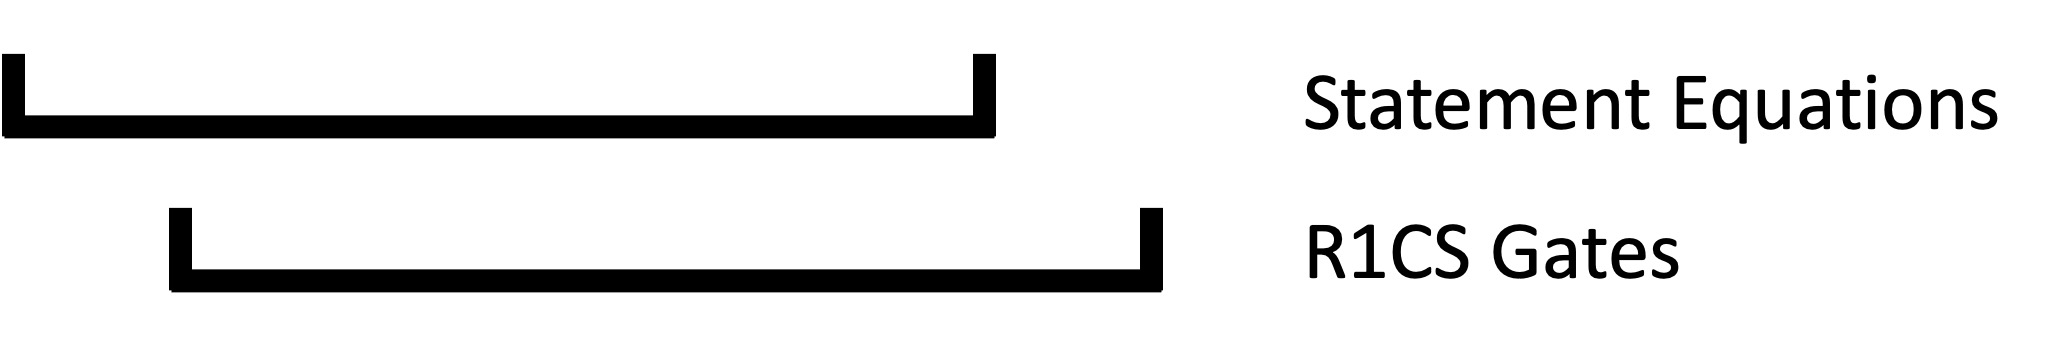
\includegraphics[width=2in]{ch-snarkprobe/figure/domain-a.jpg}
%   \vspace{-0.5cm}
  \caption{Upper Bound and Lower Bound Do Not Match}
  \label{subfig:snarkprobe-domaina}
\end{subfigure}
\hspace{0.7cm}
\vspace{0.5cm}
\begin{subfigure}{0.4\textwidth}
  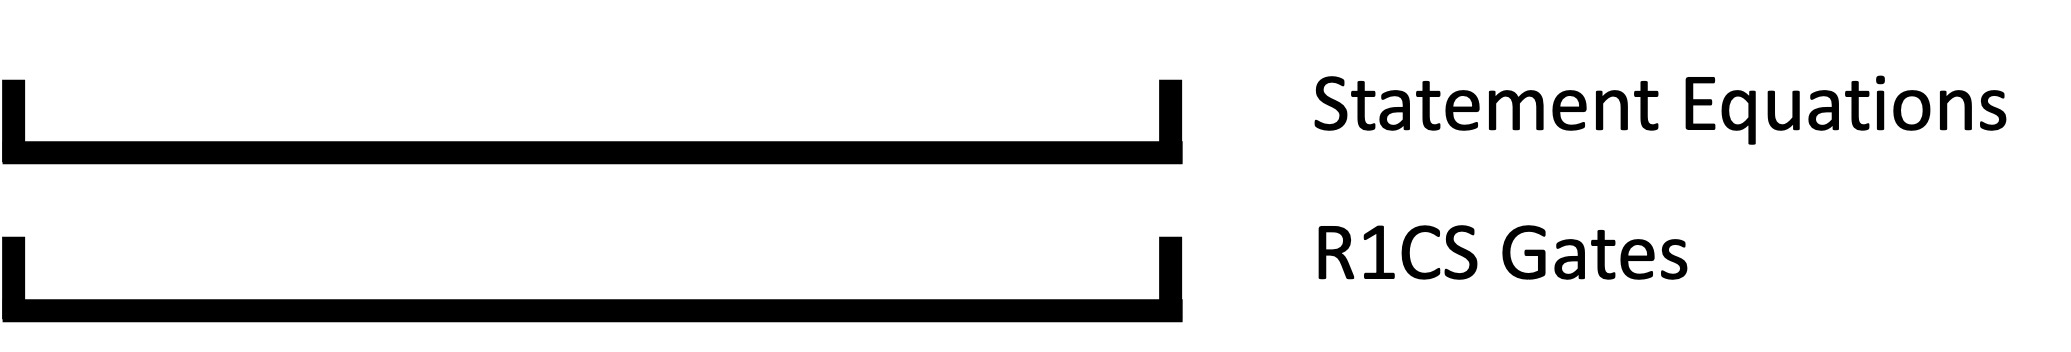
\includegraphics[width=2in]{ch-snarkprobe/figure/domain-b.jpg}
%   \vspace{-0.5cm}
  \caption{Upper Bound and Lower Bound Match}
  \label{subfig:snarkprobe-domainb}
\end{subfigure}
\begin{subfigure}{0.4\textwidth}
  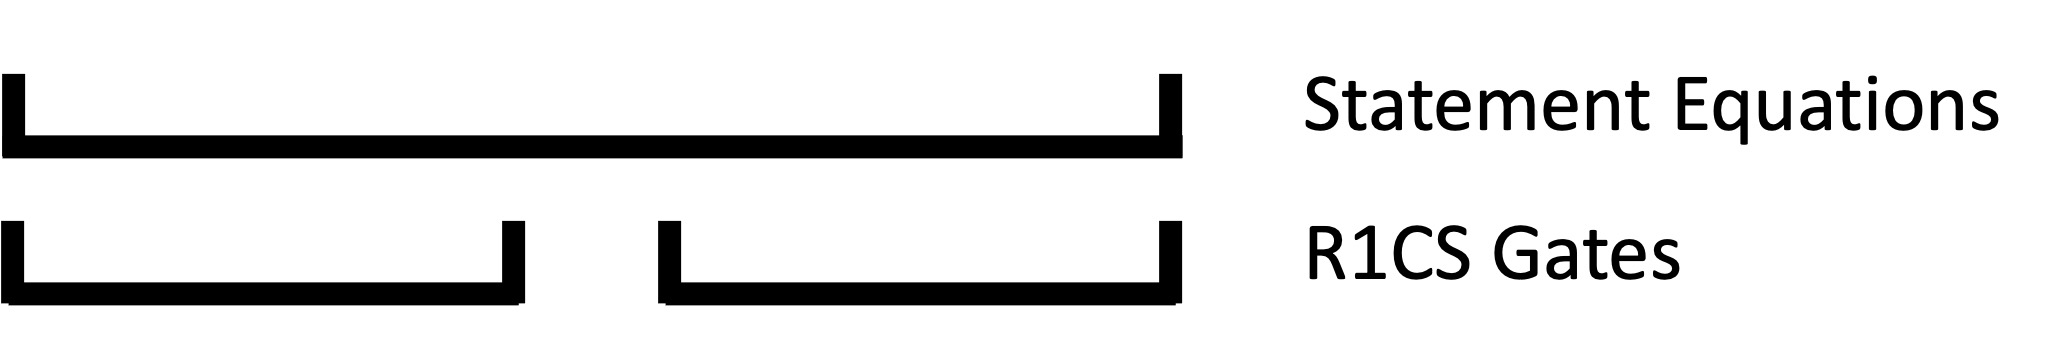
\includegraphics[width=2in]{ch-snarkprobe/figure/domain-c.jpg}
%   \vspace{-0.5cm}
  \caption{R1CS Gates Has Gap Between Bound}
  \label{subfig:snarkprobe-domainc}
\end{subfigure}
\hspace{0.7cm}
\begin{subfigure}{0.4\textwidth}
  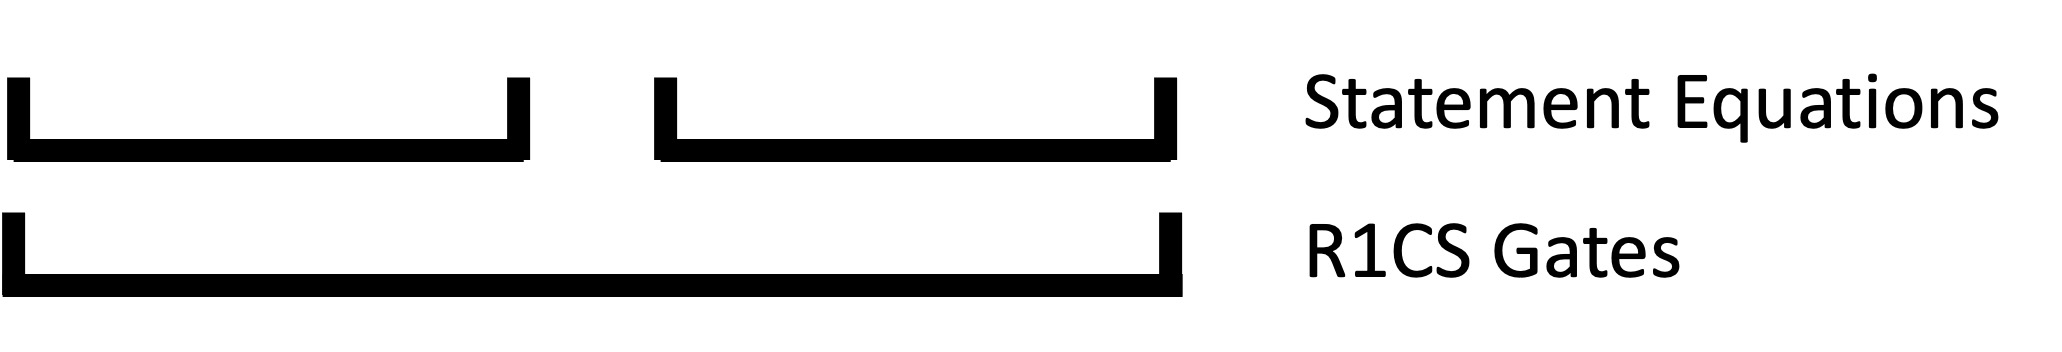
\includegraphics[width=2in]{ch-snarkprobe/figure/domain-d.jpg}
%   \vspace{-0.5cm}
  \caption{Statement Equations Has Gap Between Bound}
  \label{subfig:snarkprobe-domaind}
\end{subfigure}
\caption{Examples of Domain Comparison}
\label{fig:snarkprobe-domain}
%%\vspace{-3mm}
\end{figure}

%\newpage

%%%%%%%%%%

%\section{Comparison Between Standard Fuzzing and \SnarkFuzzer}
%
%\begin{figure}[h]
%\centering
%%\captionsetup{justification=centering}
%\begin{subfigure}{0.4\textwidth}
  %\includegraphics[width=3in]{imgs/fuzzing-a.jpg}
  %\vspace{-0.5cm}
  %\caption{Standard Fuzzing Test Procedure}
  %\label{subfig:snarkprobe-fuzzing1}
%\end{subfigure}
%\begin{subfigure}{0.4\textwidth}
  %\includegraphics[width=3in]{imgs/fuzzing-b.jpg}
  %\vspace{-0.5cm}
  %\caption{\SnarkFuzzer Procedure}
  %\label{subfig:snarkprobe-fuzzing2}
%\end{subfigure}
%\vspace{-0.2cm}
%\caption{Procedure Differences Between Standard Fuzzing Test and \SnarkFuzzer}
%\label{fig:snarkprobe-fuzzing}
%%%\vspace{-3mm}
%\end{figure}

%\newpage

%%%%%%%%%%

%\newpage

%%%%%%%%%%

%%%%%%%%%%

% \section{Additional Performance Results}
% \label{app:snarkprobe-additionalgraphs}

% \parhead{Performance of the \inputgenerator.}
% Unlike a mutation-based or generation-based fuzzer for an invalid matrix (which are very quick since they only require straightforward operations), generating a valid R1CS matrix with our generation-based fuzzer requires the SMT solver to produce a matrix based on the random witness array. Thus the processing time depends on the matrix size and random value(s) in the witness list, which generally results in a larger matrix taking longer to process.
% To validate this, we used our various fuzzers to produce matrices of varying sizes (remember that the rows represent the number of constraints and columns the number of variables). In Table \ref{tab:gen-invalid}, we present the processing time for each method (generally under one second for most methods), which confirms our general intuition.
% We also note that the \inputgenerator must compile the input matrix (proof) and source code into a binary program, which can require substantial time that is outside of our control.
% %Some \zksnark libraries may require longer compiling time, and we have no control to the library compiling time cost, which will increase our \inputgenerator total runtime.
% %\delete{ Although a larger matrix usually takes a longer time to generate, a ``smaller'' R1CS matrix may also require greater computational resources depending on the random numbers chosen in the witness and R1CS relations, as this can cause simplified relations in R1CS matrix and witness, thus requiring the SMT solver to take less time to calculate a valid R1CS matrix.\yuquan{Might need better explanation for this line?}  For example, we can see that matrix three and matrix seven in the 10 × 200 category only take roughly ten seconds to generate, which is similar to generating a matrix of size 20 × 40.} \fanyo{(summary)}

% %\begin{figure}[t]
%   %\centering
%   %%\captionsetup{justification=centering}
%   %\includegraphics[width=0.9\linewidth]{imgs/gen-invalid.jpg}
%   %\caption{Runtime of the \inputgenerator to produce R1CS matrices of different sizes.}
%   %\label{fig:snarkprobe-gen-invalid}
% %\end{figure}

% \begin{table}[h]
% %\captionsetup{justification=centering}
% \hspace*{0.15in}
% \begin{minipage}{\textwidth}
% \centering
% {\origfootnotesize
% \begin{tabular}{ll||c|c|c|c}
% \hline
% \multicolumn{2}{l||}{Matrix Size} & 5 × 10 & 20 × 40 & 50 × 100 & 50 × 200 \\ \hline\hline
% \multicolumn{1}{l||}{\multirow{2}{*}{}Generation Based} & Invalid Matrix & \textless{}0.01 & \textless{}0.01 & \textless{}0.01 & 0.02 \\ \cline{2-6}
% \multicolumn{1}{l||}{} & Valid Matrix & 0.16 & 2.06 & 23.02 & 51.27 \\ \hline
% \multicolumn{1}{l||}{\multirow{2}{*}{}Mutation Based} & Invalid Matrix & 0.38 & 0.49 & 0.65 & 0.77 \\ \cline{2-6}
% \multicolumn{1}{l||}{} & Valid Matrix & \textless{}0.01 & \textless{}0.01 & \textless{}0.01 & 0.02 \\ \hline
% \end{tabular}
% }
% \end{minipage}
% \caption{Runtime (in seconds) of the \inputgenerator to produce R1CS matrices of different sizes.}
% \label{tab:snarkprobe-gen-invalid}
% \vspace*{-14pt}
% \end{table}

% %%%%

% \parhead{Performance of the \branchmodel.}
% Next, we explore the coverage ability of the \branchmodel in terms of breadth, as well as how quickly we achieve a high percentage of branch coverage.  We ran 50 iterations of the \branchmodel with \libsnark, which covers more than 85\% of all branches.  We stopped our experiments after 50 iterations as \SnarkFuzzer did not reach any new branches over the previous 10 prior iterations.  Even with this, we note that after roughly 30 iterations we see the breadth of our coverage begin to taper off.
% A graph can be found in Figure \ref{fig:coverage}.
% %\fanyo{Even the \tool have covered most pf the branches in the target libraries, the fuzzer should not be stopped in order to generate more different inputs to test a same branch. The fuzzer should not be stopped until most of the branches have been tested for at least one time. As more inputs are generated, \tool has higher chance to find the potential issues in the target library or higher confidence to say (need a better word) that the target library is safe. }
% %There are a number of factors that can affect our coverage results. First, we can encounter situations where the generation-based fuzzer cannot produce enough diverse input sets to cover all branches, which is where the seeds of the mutation-based fuzzer can play an important role in coverage.  Second, \SnarkFuzzer allows a user to configure the proportion of matrices generated by each sub-fuzzing method, which can also affect the coverage result. In our experiment, we had the generation-based fuzzer produce 5\% invalid and 45\% valid matrices, and the mutation-based fuzzer produce 40\% invalid and 10\% valid matrices. Increasing the fuzzing time and/or adding extra seeds for the mutation-based fuzzer can improve the coverage of a target source library.

% \begin{figure}[h]
%   \centering
%   %\captionsetup{justification=centering}
%   
\includegraphics[width=0.70\linewidth]{imgs/coverage.jpg}
%   \vspace*{-10pt}
%   \caption{Percentage (breadth) of library coverage after a given number of iterations}
%   \label{fig:snarkprobe-coverage}
%   %\vspace*{-8pt}
% \end{figure}

% %%%%%%%%%%



  % Notes and footnotes are optional.
  % Reference: TM2017 page 34.
  % I have not implemented this yet.  Mark Senn 2002-06-03

  % A vita is optional for masters theses
  % and required for doctoral dissertations.
  % Reference: TM2017 page 13.
  % \include{ap-vita}

  % Listing or including publications(s) is optional.
% \include{ap-publications}
% \includepdf[scale=0.9, pages=1]{ztemp-sgopalsa-paper.pdf}
% \includepdf[offset=-1.5truein 0.25truein, scale=0.9, pages=1]{ztemp-sgopalsa-paper.pdf}
% \includepdf[offset=-1.5truein 0.2truein,  scale=0.9, pages=2]{ztemp-sgopalsa-paper.pdf}
% \includepdf[offset=-1.5truein 0.2truein,  scale=0.9, pages=3]{ztemp-sgopalsa-paper.pdf}
% \includepdf[offset=-1.5truein 0.2truein,  scale=0.9, pages=4]{ztemp-sgopalsa-paper.pdf}
% \includepdf[offset=-1.5truein 0.2truein,  scale=0.9, pages=5]{ztemp-sgopalsa-paper.pdf}
% \includepdf[offset=-1.5truein 0.2truein,  scale=0.9, pages=6]{ztemp-sgopalsa-paper.pdf}
% \includepdf[offset=-1.5truein 0.2truein,  scale=0.9, pages=7]{ztemp-sgopalsa-paper.pdf}

  % Print the index.
  % The index is optional.
  \pdfbookmark{INDEX}{index}
  \printindex

  % If \ZZshowcolophon is true, print the colophon.
  \pdfbookmark{COLOPHON}{colophon}
  \ifthen{\equal{true}{\ZZshowcolophon}}
    {\include{ap-colophon}}

% LaTeX won't read after the \end{document} command.
% You can put notes to yourself or LaTeX input not
% ready for use after "\end{document}" if you'd like.
\end{document}
